% Latex header for doxygen 1.8.4
\documentclass[twoside]{book}

% Packages required by doxygen
\usepackage{calc}
\usepackage{doxygen}
\usepackage{graphicx}
\usepackage[utf8]{inputenc}
\usepackage{makeidx}
\usepackage{multicol}
\usepackage{multirow}
\usepackage{textcomp}
\usepackage[table]{xcolor}

% Font selection
\usepackage[T1]{fontenc}
\usepackage{mathptmx}
\usepackage[scaled=.90]{helvet}
\usepackage{courier}
\usepackage{amssymb}
\usepackage{sectsty}
\renewcommand{\familydefault}{\sfdefault}
\allsectionsfont{%
  \fontseries{bc}\selectfont%
  \color{darkgray}%
}
\renewcommand{\DoxyLabelFont}{%
  \fontseries{bc}\selectfont%
  \color{darkgray}%
}

% Page & text layout
\usepackage{geometry}
\geometry{%
  a4paper,%
  top=2.5cm,%
  bottom=2.5cm,%
  left=2.5cm,%
  right=2.5cm%
}
\tolerance=750
\hfuzz=15pt
\hbadness=750
\setlength{\emergencystretch}{15pt}
\setlength{\parindent}{0cm}
\setlength{\parskip}{0.2cm}
\makeatletter
\renewcommand{\paragraph}{%
  \@startsection{paragraph}{4}{0ex}{-1.0ex}{1.0ex}{%
    \normalfont\normalsize\bfseries\SS@parafont%
  }%
}
\renewcommand{\subparagraph}{%
  \@startsection{subparagraph}{5}{0ex}{-1.0ex}{1.0ex}{%
    \normalfont\normalsize\bfseries\SS@subparafont%
  }%
}
\makeatother

% Headers & footers
\usepackage{fancyhdr}
\pagestyle{fancyplain}
\fancyhead[LE]{\fancyplain{}{\bfseries\thepage}}
\fancyhead[CE]{\fancyplain{}{}}
\fancyhead[RE]{\fancyplain{}{\bfseries\leftmark}}
\fancyhead[LO]{\fancyplain{}{\bfseries\rightmark}}
\fancyhead[CO]{\fancyplain{}{}}
\fancyhead[RO]{\fancyplain{}{\bfseries\thepage}}
\fancyfoot[LE]{\fancyplain{}{\bfseries\scriptsize \thepage }}
\fancyfoot[CE]{\fancyplain{}{}}
\fancyfoot[RE]{\fancyplain{}{}}
\fancyfoot[LO]{\fancyplain{}{}}
\fancyfoot[CO]{\fancyplain{}{}}
\fancyfoot[RO]{\fancyplain{}{\bfseries\scriptsize \thepage }}
\renewcommand{\footrulewidth}{0.4pt}
\renewcommand{\chaptermark}[1]{%
  \markboth{#1}{}%
}
\renewcommand{\sectionmark}[1]{%
  \markright{\thesection\ #1}%
}

% Indices & bibliography
\usepackage{natbib}
\usepackage[titles]{tocloft}
\setcounter{tocdepth}{1}
\setcounter{secnumdepth}{5}
\makeindex

% Hyperlinks (required, but should be loaded last)
\usepackage{ifpdf}
\ifpdf
  \usepackage[pdftex,pagebackref=true]{hyperref}
\else
  \usepackage[ps2pdf,pagebackref=true]{hyperref}
\fi
\hypersetup{%
  colorlinks=true,%
  linkcolor=blue,%
  citecolor=blue,%
  unicode%
}

% Custom commands
\newcommand{\clearemptydoublepage}{%
  \newpage{\pagestyle{empty}\cleardoublepage}%
}


%===== C O N T E N T S =====

\begin{document}

% Titlepage & ToC
\hypersetup{pageanchor=false}
\pagenumbering{roman}
\begin{titlepage}
\vspace*{7cm}
\begin{center}%
{\Large F2802x Burn In Unit}\\
\vspace*{1cm}
{\large Code Reference Manual}\\
\vspace*{0.5cm}
{\small Tue Nov 5 2013}\\
\end{center}
\end{titlepage}
\clearemptydoublepage
\tableofcontents
\clearemptydoublepage
\pagenumbering{arabic}
\hypersetup{pageanchor=true}

%--- Begin generated contents ---
\chapter{Introduction}
\label{index}\hypertarget{index}{}This document forms the reference manual for the Burn In Unit based on the Texas Instruments F2802x.

This system has been implemented using several Texas Instruments libraries; digital power v3.\-1, S\-Gen V1.\-01, I\-Q\-Math v1.\-5c and S\-Q\-Math. Please refer to the T\-I documentation pertaining to those libraries and to the C28x device to understand their operation.

This system also uses the System for Standard Commands for Programmable Instruments for C28x, again, refer to the documentation pertaining to that system to understand its use.\hypertarget{index_genop}{}\section{General Operation}\label{index_genop}
This system operates using the concept of a state machine with multiplexed threading. This allows important tasks, such as signal generation and the monitoring of critical parameters to take precedence while still allowing other less critical tasks to run with acceptable frequency. This is allowed by creating several threads D\-P\-L, A, B and C and iterating them at different interval periods, such that every time the thread is iterated the next single task in that thread is run.\hypertarget{index_fdplthread}{}\subsection{Fast (\-D\-P\-L) Thread}\label{index_fdplthread}
The D\-P\-L thread is the fastest thread, is coded in assembly and consists of only two tasks. It is the only thread that uses an interrupt to iterate. Thus the tasks are formed by an interrupt service routine (I\-S\-R). This allows the D\-P\-L thread to interrupt the ongoing action of any of the other threads. This means that as long as the length of time each of the tasks take to execute is less than the interval time, then the threads operation will be deterministic. It is within this thread's two tasks that the critical and time-\/sensitive actions of the program are carried out. The thread I\-S\-R is triggered by a start of conversion (S\-O\-C) signal from the master enhanced pulse width modulation (e\-P\-W\-M) peripheral. This occurs at a frequency of 33 k\-Hz. As there are two tasks on the thread, the frequency of each task is 16.\-5 k\-Hz resulting in a period of 60us.\hypertarget{index_sidplthread}{}\subsection{Sequential Iteration Threads}\label{index_sidplthread}
The remaining threads (A, B, C) iterate by checking the rollover state of different C\-P\-U timers. Their operation and iteration is sequential and so less deterministic. The outline of the handling sequential iteration threads by the state machine is illustrated by the following flow diagram, where N and n rollover to A and 0, respectively whenever they reach their maximum value.


\begin{DoxyImage}
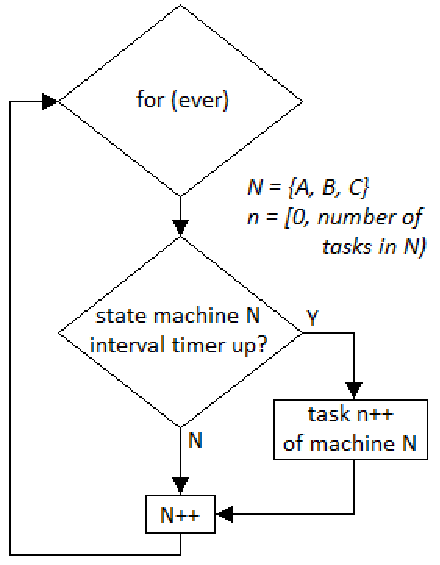
\includegraphics[width=5cm]{state_machine_loop}
\caption{Sequential iteration thread state machine}
\end{DoxyImage}


The frequency of tasks can be determined from the period of the interval timers using the following equation, where {\itshape n} is the number of tasks in the thread and {\itshape T$_{\mbox{in}}$ } is the interval timer period. \[ f_{ta}= \frac{1}{T_{in} \times n} \] With interval periods such that {\itshape T$_{\mbox{A}}$ } {\ttfamily $<$} {\itshape T$_{\mbox{B}}$ } {\ttfamily $<$} {\itshape T$_{\mbox{A}}$ } this results in the flow of execution illustrated by the following figure.


\begin{DoxyImage}
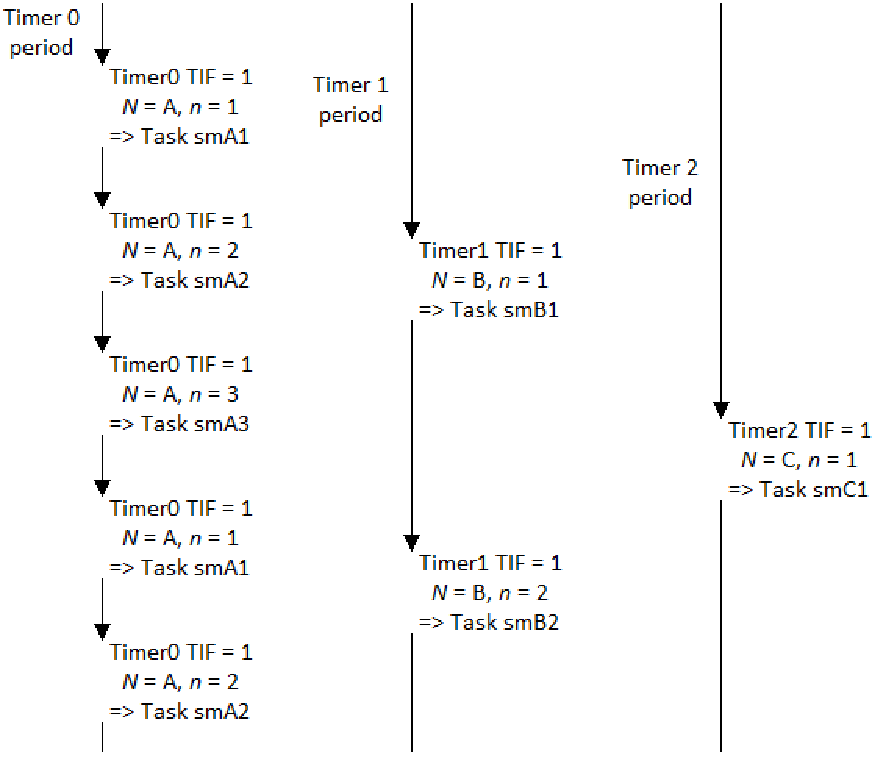
\includegraphics[width=8cm]{seq_state_machine_task_itr}
\caption{Sequence of thread tasks}
\end{DoxyImage}
\hypertarget{index_dpctrl}{}\section{Digital Power Control}\label{index_dpctrl}
The control of the power, voltage and current is managed using control loop logic, normally one loop for each stage (Transformer, A\-C, each of the four loads). These control loops are formed from a set of macros and helper functions.

Each of these macros acts as a block of functionality, much like a black-\/box electronic component, allowing their terminals to be wired together in the required order with nets. Once initialised and configured, or connected, correctly the macro blocks are executed, sequentially, by calling the appropriate code from an assembly I\-S\-R. In this case, this is what forms the D\-P\-L I\-S\-R tasks. Each block performs a precisely defined computation and delivers the result to the appropriate net-\/list variables. Each control loop's net vairables and operation parameter variables are grouped together and stored in a structure (\hyperlink{a00003}{channel\-Parameters}), with one such structure for each control loop.

The basic use of macros that are available within the program can be broken down into three parts\-:
\begin{DoxyEnumerate}
\item Initialisation\-: the macro blocks are initialised from the program by using a C callable function, D\-P\-L\-\_\-\-Init(), which is contained within the assembly file D\-P\-L\-\_\-\-I\-S\-R.\-asm.
\item Configuration\-: C pointers of the macro block terminals are assigned to net nodes to form the desired control structure, i.\-e., the control loop.
\item Execution\-: Macro block code is executed in the assembly I\-S\-R, \hyperlink{a00026_a5532a53363218854b0e4b15049d773f7}{D\-P\-L\-\_\-\-I\-S\-R()}.
\end{DoxyEnumerate}\hypertarget{index_blctrl}{}\subsection{Boost Load Control}\label{index_blctrl}
The following figure shows a diagram that illustrates the macro and net view of the control loop for one of the load boost converter stages. The loop depicted is current controlled. It uses a macro to retrieve a reading from an A\-D\-C peripheral to obtain a value that indicates the level of the current at the low side of the load input, C\-H\-A\-Nn I$_{\mbox{S\-N\-S}}$ . This value is used as the feedback into a 2-\/pole 2-\/zero filter macro where it is compared to the user-\/set reference value and the output value is varied up or down, using the filter coefficients, as needed to move it towards matching the reference. This output value is then used by another macro to set the duty of the e\-P\-W\-M peripheral that controls the switching of the converter, C\-H\-A\-Nn P\-W\-M.

Another macro retrieves a value from a second A\-D\-C that represents the voltage level across the load input, C\-H\-A\-Nn V$_{\mbox{S\-N\-S}}$ . A task in one of the sequential iteration threads compares this value to the user-\/set allowable voltage limit, the O\-V\-P limit. If the value is above this limit the control loop output is disabled and an over-\/current protection alert is raised.


\begin{DoxyImage}
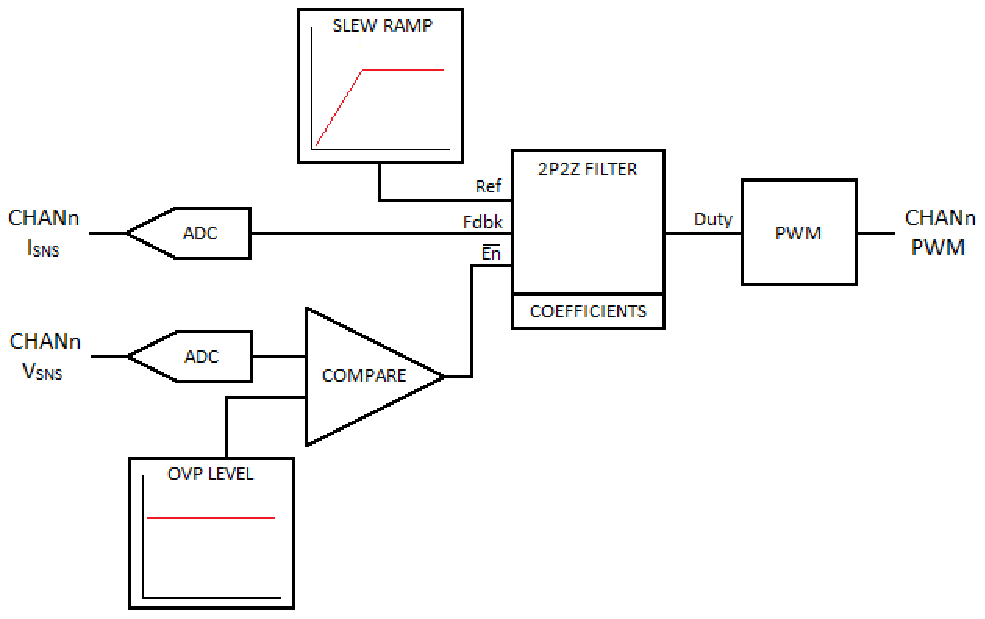
\includegraphics[width=10cm]{boost_load_loop}
\caption{Macro view of control loop for single boost load}
\end{DoxyImage}
\hypertarget{index_ibctrl}{}\subsection{Inter-\/\-Boost Control}\label{index_ibctrl}
The following figure shows a diagram that illustrates the macro and net view of the control loop for the inter-\/boost, or \char`\"{}middle\char`\"{}, boost converter stage. The loop depicted is voltage controlled. It uses a macro to retrieve a reading from an A\-D\-C peripheral to obtain a value that indicates the level of the voltage across the stage output, D\-C H\-V V$_{\mbox{S\-N\-S}}$ . This value is used as the feedback into a 3-\/pole 3-\/zero filter macro where it is compared to the user-\/set reference value and the output value is varied up or down, using the filter coefficents, as needed to move towards matching the reference. This output value is then used by another macro to set the duty of the e\-P\-W\-M peripheral that controls the switching of the converter, I\-N\-T\-B\-S\-T P\-W\-M.

Another macro retrieves a value from a second A\-D\-C that represents the current level at the low side of the input, D\-C M\-I\-D I$_{\mbox{S\-N\-S}}$ . An on-\/board analogue comparator compares this value against the user-\/set allowable current limit, the O\-C\-P limit. If the value is above this limit the comparator output sets the related trip-\/zone, quickly disabling the control loop output in software and hardware, H\-V E\-N.


\begin{DoxyImage}
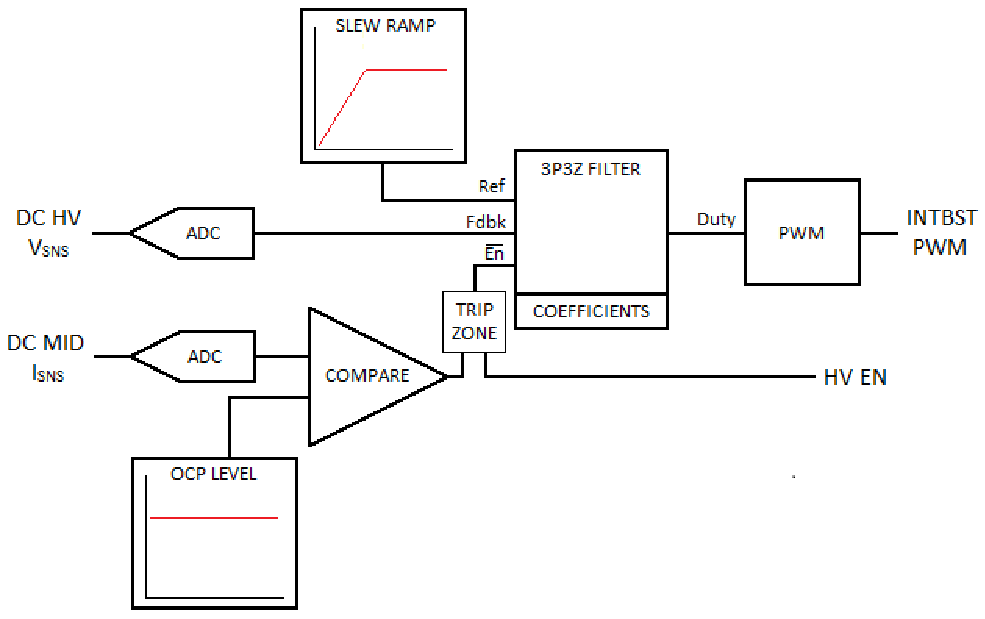
\includegraphics[width=10cm]{boost_xfmr_loop}
\caption{Macro view of control loop for inter-\/boost}
\end{DoxyImage}
\hypertarget{index_acbctrl}{}\subsection{A\-C Bridge Control}\label{index_acbctrl}
The following figure shows a diagram that illustrates the macro and a net view of the control loop for the A\-C bridge converter stage. The loop depicted is both voltage {\itshape and} current controlled. It uses a macro to retrieve a reading from an A\-D\-C peripheral to obtain a value that indicates the voltage level across the stage output, A\-C V$_{\mbox{S\-N\-S}}$ . This value is used as the feedback into a 3-\/pole 3-\/zero filter macro where it is compared to the generated sine wave reference and the output value is varied up or down, using the filter coefficients, as needed to move towards matching the reference.

Another macro retrieves a value from a second A\-D\-C that represents the current level at the low side of the stage input, A\-C I$_{\mbox{S\-N\-S}}$ . This value is used as the feedback into a 2-\/pole 2-\/zero filter macro where it is compared to the output of the 3-\/pole 3-\/zero filter macro and the output is varied up or down, using the filter coefficents, as needed to move towards matching the reference.

An on board analogue comparator also compares this A\-C I$_{\mbox{S\-N\-S}}$  value against the user-\/set allowable current limit, the O\-C\-P limit. If the value is above the limit, the comparator output sets the related trip zone, quickly disabling the control loop output and all other stages output, S\-T\-O\-P A\-L\-L.


\begin{DoxyImage}
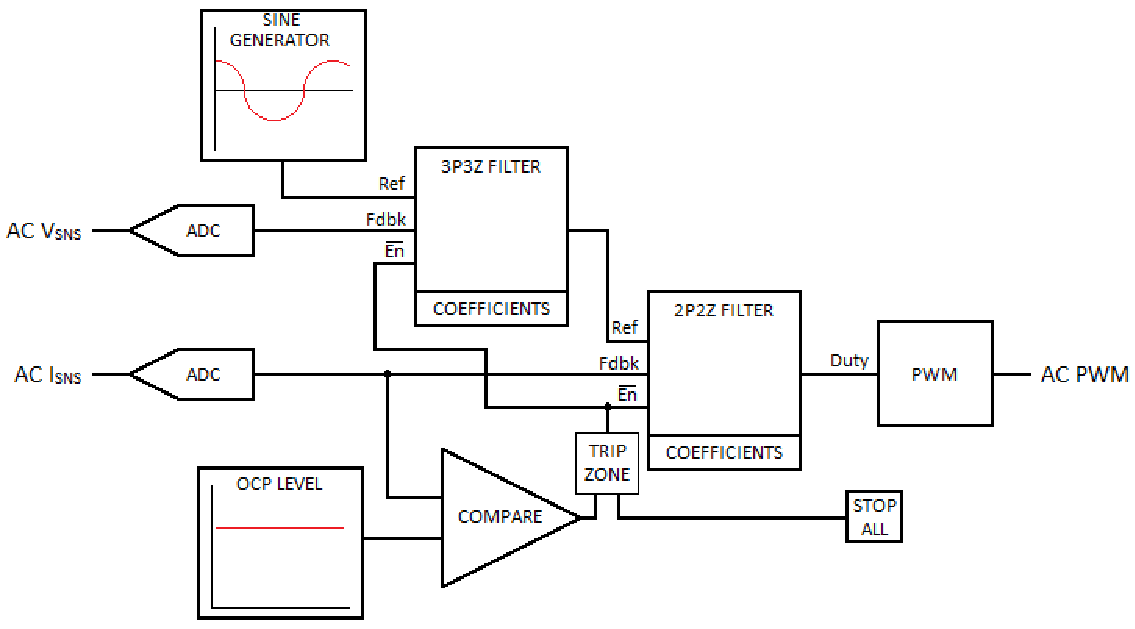
\includegraphics[width=10cm]{ac_bridge_loop}
\caption{Macro view of control loop for A\-C bridge}
\end{DoxyImage}
 
\chapter{Unit Programming}
\label{uprog}
\hypertarget{uprog}{}
\hypertarget{a00001_lang}{}\section{Language}\label{a00001_lang}
For remote programmming operations the burn in unit uses commands that follow the S\-C\-P\-I syntax as outlined in the System for Standard Commands for Programmable Instruments for C28x Code Reference Manual, where in the standard programmming commands that are included by this system are also outlined. Please refer to that document and, where necessray, any further referenced documents, for inforrmation on the syntax of the programming commands.

This unit programming chapter will focus on the function of the commands specific to the burn in unit\hypertarget{a00001_format}{}\subsection{Format}\label{a00001_format}
The burn in unit uses a standard raw T\-C\-P/\-I\-P Ethernet connection to communicate with a controlling system. Once the user's control system has established a valid raw T\-C\-P/\-I\-P connection with the burn in unit commands should be sent and received as A\-S\-C\-I\-I character byte string data, with the most significant byte first.

Thus the data sent that would correspond to the {\ttfamily $<$}C\-O\-M\-M\-O\-N Q\-U\-E\-R\-Y P\-R\-O\-G\-R\-A\-M H\-E\-A\-D\-E\-R{\ttfamily $>$} {\ttfamily $\ast$\-I\-D\-N}?; in transmission order would be (including the '$^\wedge$\-N\-L' {\ttfamily $<$}P\-R\-O\-G\-R\-A\-M M\-E\-S\-S\-A\-G\-E T\-E\-R\-M\-I\-N\-A\-T\-O\-R{\ttfamily $>$}) \begin{quotation}
{\ttfamily 0x2\-A 0x49 0x44 0x4\-E 0x3\-F 0x3\-B 0x0\-A}

\end{quotation}
\hypertarget{a00001_progcreation}{}\subsection{Program Message Unit Creation}\label{a00001_progcreation}
The user may create a {\ttfamily $<$}P\-R\-O\-G\-R\-A\-M M\-E\-S\-S\-A\-G\-E U\-N\-I\-T{\ttfamily $>$} by traversing the command tree from the root towards the desired function and concatenating the {\ttfamily $<$}program mnemonic{\ttfamily $>$}s and {\ttfamily $<$}C\-O\-M\-M\-A\-N\-D P\-R\-O\-G\-R\-A\-M H\-E\-A\-D\-E\-R{\ttfamily $>$} or {\ttfamily $<$}Q\-U\-E\-R\-Y P\-R\-O\-G\-R\-A\-M H\-E\-A\-D\-E\-R{\ttfamily $>$} stepped through to reach that destination.

For example, using the hypothetical command tree shown in the following figure, the {\ttfamily $<$}P\-R\-O\-G\-R\-A\-M M\-E\-S\-S\-A\-G\-E U\-N\-I\-T{\ttfamily $>$} required to run the function 'E\-E\-E' would be\-: \begin{quotation}
{\ttfamily B\-B\-B\-:E\-E\-E;}

\end{quotation}


\begin{center}

\begin{DoxyImageNoCaption}
  \mbox{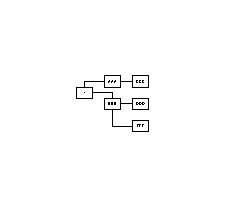
\includegraphics[width=\textwidth,height=\textheight/2,keepaspectratio=true]{dot_inline_dotgraph_1}}
\end{DoxyImageNoCaption}
\end{center}
\hypertarget{a00001_queries}{}\subsection{Queries and Responses}\label{a00001_queries}
Each {\ttfamily $<$}P\-R\-O\-G\-R\-A\-M M\-E\-S\-S\-A\-G\-E{\ttfamily $>$} may contain only one {\ttfamily $<$}Q\-U\-E\-R\-Y P\-R\-O\-G\-R\-A\-M H\-E\-A\-D\-E\-R{\ttfamily $>$} which, if used, should be the last header in the message. If a {\ttfamily $<$}Q\-U\-E\-R\-Y P\-R\-O\-G\-R\-A\-M H\-E\-A\-D\-E\-R{\ttfamily $>$} is used the next operation should be to read the response generated by the query, before any further {\ttfamily $<$}P\-R\-O\-G\-R\-A\-M M\-E\-S\-S\-A\-G\-E{\ttfamily $>$} elements are sent to the unit.\hypertarget{a00001_device}{}\section{Instrument Selection}\label{a00001_device}
Each burn in unit is split into several logical instruments that corresponds to the functional sections of the burn in unit. The instruement selection is controlled using the {\ttfamily I\-N\-S\-Trument} subssytem These instruments are numbered according to the unit channel numbering shown in the following list. These numbers can be obtained by using the {\ttfamily C\-A\-Talog}? query from the {\ttfamily I\-N\-S\-Trument} subsystem\-: \begin{quotation}
{\ttfamily I\-N\-S\-Trument\-:C\-A\-Talog?;}.

\end{quotation}


\begin{enumerate}\setcounter{enumi}{-1} \item Load 0 \item Load 1 \item Load 2 \item Load 3 \item AC Current Control \item DC Stage \item AC Stage \end{enumerate}

This means that before setting any of the instruments' settings, the relevant instrument number must first be selected. This is done using the {\ttfamily N\-S\-E\-Lect} command from the {\ttfamily I\-N\-S\-Trument} subsystem. The default instrument selection is 0. Once selected the value is \char`\"{}sticky\char`\"{}, and does not need to be set again until the user settings wishes to send commands for a different instrument. Thus, for example, the {\ttfamily $<$}P\-R\-O\-G\-R\-A\-M M\-E\-S\-S\-A\-G\-E{\ttfamily $>$} required to set the voltage level D\-C stage to 10 volts with a range set to 1\-V/\-V would be as follows\-: \begin{quotation}
{\ttfamily I\-N\-S\-Trument\-:N\-S\-E\-Lect 5;\-:S\-O\-U\-Rce\-:\-V\-O\-L\-Tage\-:L\-E\-Vel 10;\-:S\-O\-U\-Rce\-:\-V\-O\-L\-Tage\-:R\-A\-N\-Ge 1;}

\end{quotation}
\hypertarget{a00001_tree}{}\section{The Command Tree}\label{a00001_tree}
The command tree provides the structure of the subsystems and their commands. As shown however the diagram does not illustrate that some of the commands have no meaning to some instruments. For example, attempting to set the voltage coefficients of a current controlled instrument will result in an error.

Again, the commands shown here are in addition to those that are implemented as standard by the System for Standard Commands for Programmable Instruments for C28x.

The diagram is followed by a listing of each command. The next section, \hyperlink{a00002}{Command Reference} explains the operation and details of each command.

\begin{center}

\begin{DoxyImageNoCaption}
  \mbox{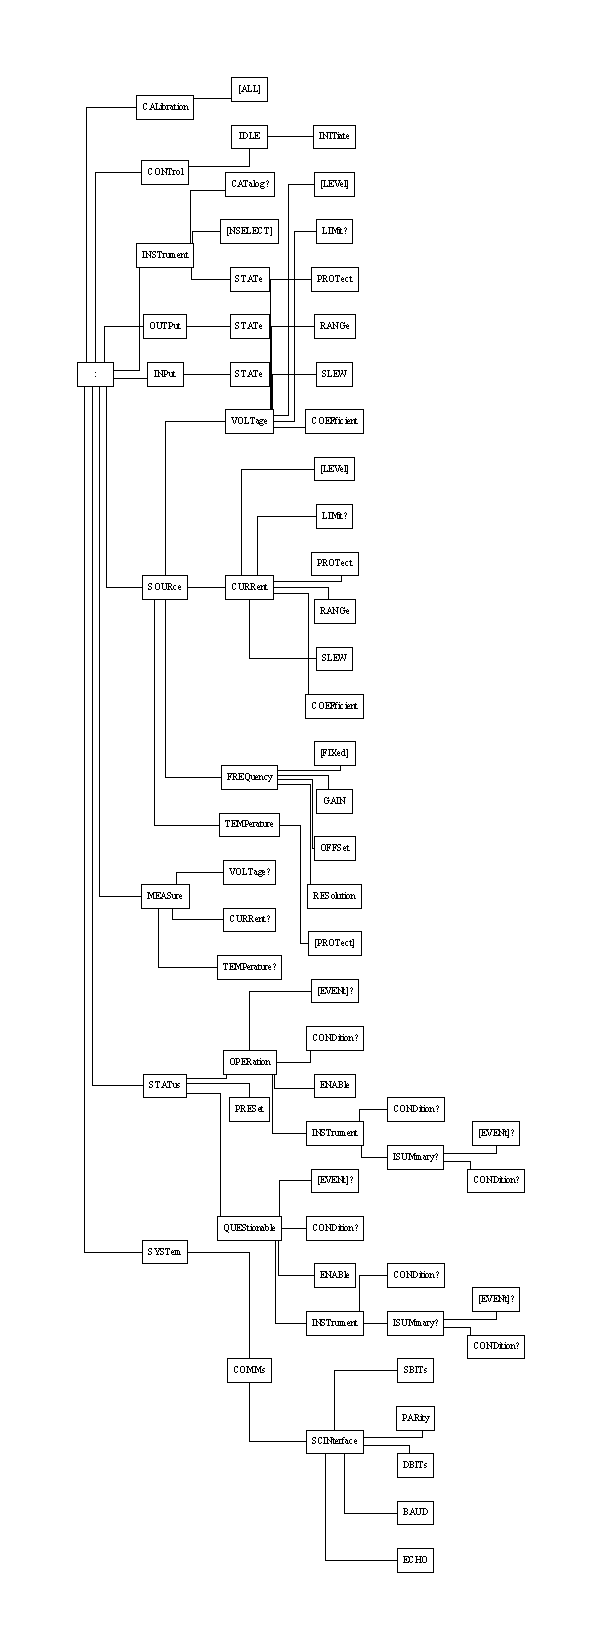
\includegraphics[width=\textwidth,height=\textheight/2,keepaspectratio=true]{dot_inline_dotgraph_2}}
\end{DoxyImageNoCaption}
\end{center}



\begin{DoxyPre}
{\bfseries CALibration}
    ALL
{\bfseries CONTrol}
    IDLE
        INITiate
{\bfseries INSTrument}
    CATalog?
    NSELect
    STATe
{\bfseries OUTPut}
    STATe
{\bfseries INPut}
    STATe
{\bfseries SOURce}
    VOLTage
        LEVel
        LIMit?
        PROTect
        RANGe
        SLEW
        COEFficient
    CURRent
        LEVel
        LIMit?
        PROTect
        RANGe
        SLEW
        COEFficient
    FREQuency
        FIXed
        GAIN
        OFFSet
    TEMPerature
        PROTect
{\bfseries MEASure}
    VOLTage?
    CURRent?
    TEMPerature?
{\bfseries STATus}
    OPERation
    PRESet
    QUEStionable
{\bfseries SYSTem}
    COMMs
        SCINterface
            SBITs
            PARity
            DBITs
            BAUD
            ECHO
\end{DoxyPre}
 
\chapter{Command Reference}
\label{cmdref}
\hypertarget{cmdref}{}
This section outlines the operation of each command and node on the command tree. All commands, unless otherwise specified, also have an equivalent query form that returns the value that the command is currently set to. For example, querying S\-O\-U\-Rce\-:\-V\-O\-L\-Tage\-:P\-R\-O\-Tect? will return the current voltage protection level setting.

Some commands have a query form {\itshape only}, that is they have no none-\/query form. these commands are identified by the presence of the query terminator character, '?'.

Some of the commands are optional, or default. Such optionality is represented by the presence of square brackets enclosing the command, '\mbox{[}' and '\mbox{]}'. Where commands are optional, it is possible to use the parent node alone instead of needing to append the optional child command. For example, as the \-:N\-S\-E\-Lect command from the I\-N\-S\-Trument subsystem is marked as optional, the command to select an instrument can be either\-: \begin{quotation}
{\ttfamily I\-N\-S\-Trument\-:N\-S\-E\-Lect {\ttfamily $<$}numeric\-\_\-value{\ttfamily $>$};}

\end{quotation}
or \begin{quotation}
{\ttfamily I\-N\-S\-Trument {\ttfamily $<$}numeric\-\_\-value{\ttfamily $>$};}

\end{quotation}
\hypertarget{a00002_cal}{}\section{C\-A\-Libration Subsystem}\label{a00002_cal}
This subsystem has the function of performing system calibration. Currently the subsystem has only one function, the default command A\-L\-L and it's complementing query.\hypertarget{a00002_calall}{}\subsection{\mbox{[}\-:\-A\-L\-L\mbox{]}}\label{a00002_calall}
{\ttfamily C\-A\-Libration\-:A\-L\-L}\par
 The C\-A\-Libration\-:A\-L\-L command performs the same function as the C\-A\-Libration\-:A\-L\-L? command except there is no response. Calibration errors are reported through the status-\/reporting mechanism. While this command is executing the C\-A\-Librating bit of the Operation Status Condition register will be set.\hypertarget{a00002_callallq}{}\subsection{\mbox{[}\-:\-A\-L\-L\mbox{]}?}\label{a00002_callallq}
{\ttfamily Calibration\-:A\-L\-L?}\par
 The A\-L\-L? query performs a full calibration of the instrument and responds with a {\ttfamily $<$}numeric\-\_\-value{\ttfamily $>$} indicating the success of the calibration. A zero will be returned if calibration is completed successfully; otherwise a nonzero value which represents the appropriate error number shall be returned. An instrument will still report calibration errors through the status-\/reporting mechanism, even though an error is reported by the value of the query response.\hypertarget{a00002_ctrl}{}\section{C\-O\-N\-Trol Subsystem}\label{a00002_ctrl}
The C\-O\-N\-Trol subsystem is used to turn on and off or control the state of the entire device.\hypertarget{a00002_ctrlidle}{}\subsection{\-:\-I\-D\-L\-E}\label{a00002_ctrlidle}
{\ttfamily C\-O\-N\-Trol\-:I\-D\-L\-E}\par
 This node contains commands that control the I\-D\-L\-E state of the device.\hypertarget{a00002_ctrlidleinit}{}\subsubsection{\-:\-I\-N\-I\-Tiate}\label{a00002_ctrlidleinit}
{\ttfamily C\-O\-N\-Trol\-:\-I\-D\-L\-E\-:I\-N\-I\-Tiate}\par
 Returns the device to the idle state. This command is an event and has no associated $\ast$\-R\-S\-T condition or query command.\hypertarget{a00002_inst}{}\section{I\-N\-S\-Trument Subsystem}\label{a00002_inst}
This device uses multiple logical instruments (as described in \hyperlink{a00001_device}{Instrument Selection}), this subsystem provides the mechanism to identify and select logical instruments by number.\hypertarget{a00002_instcat}{}\subsection{\-:\-C\-A\-Talog?}\label{a00002_instcat}
{\ttfamily I\-N\-S\-Trument\-:C\-A\-Talog?}\par
 The C\-A\-Talog query returns a comma-\/separated list of the numbers of all logical instruments.\hypertarget{a00002_instnsel}{}\subsection{\-:\-N\-S\-E\-Lect $<$numeric\-\_\-value$>$}\label{a00002_instnsel}
{\ttfamily I\-N\-S\-Trument\-:N\-S\-E\-Lect}\par
 This command selects an instrument according to the numeric value parameter. When a logical instrument is selected, all other logical instruments or groups are unavailable for programming until selected. When queried it shall return the selected logical instrument number.

Note that the numbering used for logical instruments directly corresponds to the numbers used in status reporting for the multiple instruments; specifically the S\-T\-A\-Tus\-:\-Q\-U\-E\-Stionable\-:I\-N\-S\-Trument and S\-T\-A\-Tus\-:\-O\-P\-E\-Ration\-:I\-N\-S\-Trument commands.

At $\ast$\-R\-S\-T, instrument 0 is selected.\hypertarget{a00002_inststat}{}\subsection{\-:\-S\-T\-A\-Te $<$\-Boolean$>$}\label{a00002_inststat}
{\ttfamily I\-N\-S\-Trument\-:S\-T\-A\-Te}\par
 Turns the selected logical instrument O\-N or O\-F\-F. A logical instrument does not have to be turned O\-F\-F before another logical instrument is selected. That is, several logical instruments may be active, while only one may be selected. When an instrument is active, measurements occur and signals are generated. When inactive, measurements do not occur and signals are not generated. When a logical instrument is selected, yet is inactive, all commands shall be processed so that the logical instrument shall reflect the state changes requested when the logical instrument is turned on.

At $\ast$\-R\-S\-T, this value is O\-F\-F.\hypertarget{a00002_outp}{}\section{O\-U\-T\-Put Subsystem}\label{a00002_outp}
The O\-U\-T\-Put subsystem controls the characteristics of the selected instrument's output port.\hypertarget{a00002_outpstat}{}\subsection{\mbox{[}\-:\-S\-T\-A\-Te\mbox{]} $<$\-Boolean$>$}\label{a00002_outpstat}
{\ttfamily O\-U\-T\-Put\-:S\-T\-A\-Te}\par
 Selects the state of the output. When S\-T\-A\-Te is O\-N the signal generated by the source is emitted from the output port of the selected instrument.\hypertarget{a00002_inp}{}\section{I\-N\-Put Subsystem}\label{a00002_inp}
The I\-N\-Put subsystem controls the characteristics of the selected instrument's input port.\hypertarget{a00002_inpstat}{}\subsection{\-:\-S\-T\-A\-Te $<$\-Boolean$>$}\label{a00002_inpstat}
{\ttfamily I\-N\-Put\-:S\-T\-A\-Te}\par
 Selects the state of the input. When S\-T\-A\-Te is O\-N the signal generated by the source is emitted from the output port of the selected instrument.\hypertarget{a00002_sour}{}\section{S\-O\-U\-Rce Subsystem}\label{a00002_sour}
The S\-O\-U\-Rce setup commands are divided into several sections. Each section or subsystem deals with controls that directly affect device-\/specific settings of the selected instrument.\hypertarget{a00002_sourvolt}{}\subsection{\-:\-V\-O\-L\-Tage}\label{a00002_sourvolt}
This subsection controls the signal voltage characteristics of the source.\hypertarget{a00002_sourvoltlev}{}\subsubsection{\mbox{[}\-:\-L\-E\-Vel\mbox{]} $<$numeric\-\_\-value$>$}\label{a00002_sourvoltlev}
{\ttfamily S\-O\-U\-Rce\-:\-V\-O\-L\-Tage\-:L\-E\-Vel}\par
 This command sets the target voltage level of a voltage controlled instrument. The numeric value parameter is the level to be set in volts, between 0 and the voltage limit returned in response the L\-I\-Mit? query.\hypertarget{a00002_sourvoltlim}{}\subsubsection{\-:\-L\-I\-Mit?}\label{a00002_sourvoltlim}
{\ttfamily S\-O\-U\-Rce\-:\-V\-O\-L\-Tage\-:L\-E\-Vel}\par
 This command has a query form only. This is because the voltage limit value is fixed. The query response is a single numeric value in volts representing this fixed limit.\hypertarget{a00002_sourvoltprot}{}\subsubsection{\-:\-P\-R\-O\-Tect $<$numeric\-\_\-value$>$}\label{a00002_sourvoltprot}
{\ttfamily S\-O\-U\-Rce\-:\-V\-O\-L\-Tage\-:P\-R\-O\-Tect}\par
 This command sets the voltage protection level. This is the level at which the over-\/voltage protection is triggered if the voltage rises above it The numeric value parameter is the level to be set in volts, between 0 and the voltage limit returned in response to the L\-I\-Mit? query.\hypertarget{a00002_sourvoltrang}{}\subsubsection{\-:\-R\-A\-N\-Ge $<$numeric\-\_\-value$>$}\label{a00002_sourvoltrang}
{\ttfamily S\-O\-U\-Rce\-:\-V\-O\-L\-Tage\-:R\-A\-N\-Ge}\par
 This command sets the voltage range. The numeric value parameter is the voltage scaling value in volts-\/per-\/volt from 0 to 1.\hypertarget{a00002_sourvoltslew}{}\subsubsection{\-:\-S\-L\-E\-W $<$numeric\-\_\-value$>$}\label{a00002_sourvoltslew}
{\ttfamily S\-O\-U\-Rce\-:\-V\-O\-L\-Tage\-:S\-L\-E\-W}\par
 This command sets the voltage slew for a voltage controlled instrument. The numeric value parameter is the voltage slew rate value in volts-\/per-\/microseconds from 0 to 1.\hypertarget{a00002_sourvoltcoef}{}\subsubsection{\-:\-C\-O\-E\-Fficient $<$numeric\-\_\-value$>$, $<$numeric value$>$}\label{a00002_sourvoltcoef}
{\ttfamily S\-O\-U\-Rce\-:\-V\-O\-L\-Tage\-:C\-O\-E\-Fficient}\par
 This command is used to specify the voltage control coefficients, of a voltage controlled instrument. The first numeric value parameter specifies the coefficient to be changed, according to the following list, while the second numeric value parameter specifies the level the selected coefficient is to be changed to.

\begin{enumerate}\setcounter{enumi}{-1} \item Saturation Minimum \item Saturation Maximum \item B0 \item B1 \item A1 \item B2 \item A2 \item B3 \item A3 \end{enumerate}

When queried, the response is a list of comma separated numeric values in the following order\-: \begin{quotation}
Saturation-\/\-Minimum-\/value, Saturation-\/\-Maximum-\/value, B0-\/value, B1-\/value, A1-\/value, B2-\/value, A2-\/value, B3-\/value, A3-\/value

\end{quotation}
\hypertarget{a00002_sourcurr}{}\subsection{\-:\-C\-U\-R\-Rent}\label{a00002_sourcurr}
{\ttfamily S\-O\-U\-Rce\-:C\-U\-R\-Rent}\par
 This subsection controls the signal current characteristics of the source.\hypertarget{a00002_sourcurrlev}{}\subsubsection{\mbox{[}\-:\-L\-E\-Vel\mbox{]} $<$numeric\-\_\-value$>$}\label{a00002_sourcurrlev}
{\ttfamily S\-O\-U\-Rce\-:\-C\-U\-R\-Rent\-:L\-E\-Vel}\par
 This command sets the target current level of a current controlled instrument. The numeric value parameter is the level to be set in amps, between 0 and the current limit returned in response the L\-I\-Mit? query.\hypertarget{a00002_sourcurrlim}{}\subsubsection{\-:\-L\-I\-Mit?}\label{a00002_sourcurrlim}
{\ttfamily S\-O\-U\-Rce\-:\-C\-U\-R\-Rent\-:L\-E\-Vel}\par
 This command has a query form only. This is because the current limit value is fixed. The query response is a single numeric value in amps representing this fixed limit.\hypertarget{a00002_sourcurrprot}{}\subsubsection{\-:\-P\-R\-O\-Tect $<$numeric\-\_\-value$>$}\label{a00002_sourcurrprot}
{\ttfamily S\-O\-U\-Rce\-:\-V\-O\-L\-Tage\-:P\-R\-O\-Tect}\par
 This command sets the current protection level. This is the level at which the over-\/current protection is triggered if the current rises above it The numeric value parameter is the level to be set in amps, between 0 and the current limit returned in response to the L\-I\-Mit? query.\hypertarget{a00002_sourcurrrang}{}\subsubsection{\-:\-R\-A\-N\-Ge $<$numeric\-\_\-value$>$}\label{a00002_sourcurrrang}
{\ttfamily S\-O\-U\-Rce\-:\-C\-U\-R\-Rent\-:R\-A\-N\-Ge}\par
 This command sets the current range. The numeric value parameter is the current scaling value in amps-\/per-\/volt from 0 to 1. {\bfseries $<$-\/-\/---!!!-\/-\/---}\hypertarget{a00002_sourcurrslew}{}\subsubsection{\-:\-S\-L\-E\-W $<$numeric\-\_\-value$>$}\label{a00002_sourcurrslew}
{\ttfamily S\-O\-U\-Rce\-:\-C\-U\-R\-Rent\-:S\-L\-E\-W}\par
 This command sets the current slew for a current controlled instrument. The numeric value parameter is the current slew rate value in amps-\/per-\/microseconds from 0 to 1.\hypertarget{a00002_sourcurrcoef}{}\subsubsection{\-:\-C\-O\-E\-Fficient $<$numeric\-\_\-value$>$, $<$numeric\-\_\-value$>$}\label{a00002_sourcurrcoef}
{\ttfamily S\-O\-U\-Rce\-:\-C\-U\-R\-Rent\-:C\-O\-E\-Fficient}\par
 This command is used to specify the current control coefficients, of a current controlled instrument. The first numeric value parameter specifies the coefficient to be changed, according to the following list, while the second numeric value parameter specifies the level the selected coefficient is to be changed to.

\begin{enumerate}\setcounter{enumi}{-1} \item Saturation Minimum \item Saturation Maximum \item B0 \item B1 \item A1 \item B2 \item A2 \end{enumerate}

When queried, the response is a list of comma separated numeric values in the following order\-: \begin{quotation}
Saturation-\/\-Minimum-\/value, Saturation-\/\-Maximum-\/value, B0-\/value, B1-\/value, A1-\/value, B2-\/value, A2-\/value

\end{quotation}
\hypertarget{a00002_sourfreq}{}\subsection{\-:\-F\-R\-E\-Quency}\label{a00002_sourfreq}
{\ttfamily S\-O\-U\-Rce\-:F\-R\-E\-Quency}\par
 The F\-R\-E\-Quency subsystem controls the frequency characteristics of an instrument source that produces a periodic signal -\/ such as the sine wave produced by the A\-C stage.\hypertarget{a00002_sourfreqfix}{}\subsubsection{\mbox{[}\-:\-F\-I\-Xed\mbox{]} $<$numeric\-\_\-value$>$}\label{a00002_sourfreqfix}
{\ttfamily S\-O\-U\-Rce\-:\-F\-R\-E\-Quency\-:F\-I\-Xed}\par
 This command is used to set the source frequency. The numeric value parameter should be the required frequency in hertz, from 0 to 1000.\hypertarget{a00002_sourfreqgain}{}\subsubsection{\-:\-G\-A\-I\-N $<$numeric\-\_\-value$>$}\label{a00002_sourfreqgain}
{\ttfamily S\-O\-U\-Rce\-:\-F\-R\-E\-Quency\-:G\-A\-I\-N}\par
 This command is used to set the frequency gain. The numeric value parameter should vary from 0 to 1\hypertarget{a00002_sourfreqoffs}{}\subsubsection{\-:\-O\-F\-F\-Set $<$numeric\-\_\-value$>$}\label{a00002_sourfreqoffs}
{\ttfamily S\-O\-U\-Rce\-:\-F\-R\-E\-Quency\-:O\-F\-F\-Set}\par
 This command sets the frequency offset. The numeric value parameter should vary between -\/0.\-5 and +0.5\hypertarget{a00002_sourtemp}{}\subsection{\-:\-T\-E\-M\-Perature}\label{a00002_sourtemp}
{\ttfamily S\-O\-U\-Rce\-:T\-E\-M\-Perature}\par
 The temperature subsystem controls the temperature of the selected logical instrument. Note that not all instruments have temperature control functionality.\hypertarget{a00002_sourtempprot}{}\subsubsection{\mbox{[}\-:\-P\-R\-O\-Tect\mbox{]} $<$numeric\-\_\-value$>$}\label{a00002_sourtempprot}
{\ttfamily S\-O\-U\-Rce\-:\-T\-E\-M\-Perature\-:P\-R\-O\-Tect}\par
 This command sets the temperature protection level. This is the level at which the over-\/temperature protection is triggered if the temperature rises above it The numeric value parameter is the level to be set in degrees Celsius, between 0 and 150 $^{\mbox{o}}$ C.\hypertarget{a00002_meas}{}\section{M\-E\-A\-Sure Subsystem}\label{a00002_meas}
The M\-E\-A\-Sure susbsytem allows the user to take measurements of certain aspects of the selected instruments operation.\hypertarget{a00002_measvolt}{}\subsection{\-:\-V\-O\-L\-Tage?}\label{a00002_measvolt}
{\ttfamily M\-E\-A\-Sure\-:V\-O\-L\-Tage?} This query responds with a numeric value of the current voltage reading from the selected instrument in volts.\hypertarget{a00002_meascurr}{}\subsection{\-:\-C\-U\-R\-Rent?}\label{a00002_meascurr}
{\ttfamily M\-E\-A\-Sure\-:C\-U\-R\-Rent?} This query responds with a numeric value of the current electrical current reading from the selected instrument in amps.\hypertarget{a00002_meastemp}{}\subsection{\-:\-T\-E\-M\-Perature?}\label{a00002_meastemp}
{\ttfamily M\-E\-A\-Sure\-:T\-E\-M\-Perature?} This query responds with a numeric value of the current temperature reading from the selected instrument in degrees Celsius.\hypertarget{a00002_stat}{}\section{S\-T\-A\-Tus Subsystem}\label{a00002_stat}
\hypertarget{a00002_statoper}{}\subsection{\-:\-O\-P\-E\-Ration}\label{a00002_statoper}
\hypertarget{a00002_statpres}{}\subsection{\-:\-P\-R\-E\-Set}\label{a00002_statpres}
\hypertarget{a00002_statques}{}\subsection{\-:\-Q\-U\-E\-Stionable}\label{a00002_statques}
\hypertarget{a00002_syst}{}\section{S\-Y\-S\-Tem}\label{a00002_syst}
The S\-Y\-S\-Tem subsystem collects the functions that are not related to instrument performance.\hypertarget{a00002_systcomm}{}\subsection{\-:\-C\-O\-M\-Ms}\label{a00002_systcomm}
{\ttfamily S\-Y\-S\-Tem\-:C\-O\-M\-Ms}\par
 This subsystem controls some aspects of the serial communications (S\-C\-I) interface.\hypertarget{a00002_systcommsbit}{}\subsubsection{\-:\-S\-B\-I\-Ts $<$numeric\-\_\-value$>$}\label{a00002_systcommsbit}
{\ttfamily S\-Y\-S\-Tem\-:\-C\-O\-M\-Ms\-:S\-B\-I\-Ts}\par
 This command sets the number of stop bits used in the S\-C\-I frame. The numeric value parameter sets the number of stop bits and may be either 1 or 2. The default value is 1.\hypertarget{a00002_systcommpar}{}\subsubsection{\-:\-P\-A\-Rity $<$numeric\-\_\-value$>$}\label{a00002_systcommpar}
{\ttfamily S\-Y\-S\-Tem\-:\-C\-O\-M\-Ms\-:P\-A\-Rity}\par
 This command sets what parity is used in the S\-C\-I frames. The defualt selection is for no parity. The numeric value parameter sets the parity in use and corresponds to parity settings as described by the following list\-:

\begin{enumerate}\setcounter{enumi}{-1} \item No parity \item Odd parity \item Even parity \end{enumerate}\hypertarget{a00002_systcommdbit}{}\subsubsection{\-:\-D\-B\-I\-Ts $<$numeric\-\_\-value$>$}\label{a00002_systcommdbit}
{\ttfamily S\-Y\-S\-Tem\-:\-C\-O\-M\-Ms\-:D\-B\-I\-Ts}\par
 This command sets how many data bits are in the S\-C\-I frame. The numeric value perameter sets the number of data bits and may vary from 1 to 8.\hypertarget{a00002_systcommbaud}{}\subsubsection{\-:\-B\-A\-U\-D $<$numeric\-\_\-value$>$}\label{a00002_systcommbaud}
{\ttfamily S\-Y\-S\-Tem\-:\-C\-O\-M\-Ms\-:B\-A\-U\-D}\par
 This command sets the baud rate used by the S\-C\-I interface. The numeric value parameter sets the baud rate. The allowed parameters are any of the standard baud rates which are listed in the table below. Acceptance of a baud rate does not indicate that the device is capable of use such a baud rate. The default baud rate is 9600.

\begin{TabularC}{3}
\hline
\rowcolor{lightgray}\PBS\centering {\bf Accepted Baud Rates }&\PBS\centering {\bf Accepted Baud Rates }&\PBS\centering {\bf Accepted Baud Rates  }\\\cline{1-3}
\PBS\centering 110 &\PBS\centering 9600 &\PBS\centering 57600 \\\cline{1-3}
\PBS\centering 300 &\PBS\centering 14400 &\PBS\centering 115200 \\\cline{1-3}
\PBS\centering 600 &\PBS\centering 19200 &\PBS\centering 230400 \\\cline{1-3}
\PBS\centering 1200 &\PBS\centering 28800 &\PBS\centering 460800 \\\cline{1-3}
\PBS\centering 2400 &\PBS\centering 38400 &\PBS\centering 921600 \\\cline{1-3}
\PBS\centering 4800 &\PBS\centering 56000 &\PBS\centering \\\cline{1-3}
\end{TabularC}
\hypertarget{a00002_systcommecho}{}\subsubsection{\-:\-E\-C\-H\-O $<$\-Boolean$>$}\label{a00002_systcommecho}
{\ttfamily S\-Y\-S\-Tem\-:\-C\-O\-M\-Ms\-:E\-C\-H\-O}\par
 This command enables or disables the echo functionality of the S\-C\-I interface. If the boolean parameter is O\-N the interface echos any data it receives without passing that data on to any other part of the device. The default setting is O\-F\-F. 
\chapter{Data Structure Documentation}
\hypertarget{a00003}{\section{ac\-Stage\-Nets Struct Reference}
\label{a00003}\index{ac\-Stage\-Nets@{ac\-Stage\-Nets}}
}


{\ttfamily \#include $<$Macro\-Nets.\-h$>$}

\subsection*{Data Fields}
\begin{DoxyCompactItemize}
\item 
volatile int32 \hyperlink{a00003_a60c47bf62f481657a9548acf5115bdcc}{v\-Ref\-Net}
\item 
volatile int32 \hyperlink{a00003_a2fa47f230edc315908ef3c7594572d40}{v\-Fdbk\-Net}
\item 
volatile int32 \hyperlink{a00003_a4e528cf0beafdcc7ab51f05980c719b3}{i\-Fdbk\-Net}
\item 
volatile int32 \hyperlink{a00003_aef9fb780c943a15cfcf991e330f13d26}{i\-Ref\-Net}
\item 
volatile int32 \hyperlink{a00003_a4d5d9d0263738ce9262cdbd4db0e404b}{i\-Filt\-Out\-Net}
\end{DoxyCompactItemize}


\subsection{Detailed Description}
A structure that contains the nets used in the A\-C stage. 

\subsection{Field Documentation}
\hypertarget{a00003_a4e528cf0beafdcc7ab51f05980c719b3}{\index{ac\-Stage\-Nets@{ac\-Stage\-Nets}!i\-Fdbk\-Net@{i\-Fdbk\-Net}}
\index{i\-Fdbk\-Net@{i\-Fdbk\-Net}!acStageNets@{ac\-Stage\-Nets}}
\subsubsection[{i\-Fdbk\-Net}]{\setlength{\rightskip}{0pt plus 5cm}volatile int32 ac\-Stage\-Nets\-::i\-Fdbk\-Net}}\label{a00003_a4e528cf0beafdcc7ab51f05980c719b3}
Current feedback net (I\-Q24). \hypertarget{a00003_a4d5d9d0263738ce9262cdbd4db0e404b}{\index{ac\-Stage\-Nets@{ac\-Stage\-Nets}!i\-Filt\-Out\-Net@{i\-Filt\-Out\-Net}}
\index{i\-Filt\-Out\-Net@{i\-Filt\-Out\-Net}!acStageNets@{ac\-Stage\-Nets}}
\subsubsection[{i\-Filt\-Out\-Net}]{\setlength{\rightskip}{0pt plus 5cm}volatile int32 ac\-Stage\-Nets\-::i\-Filt\-Out\-Net}}\label{a00003_a4d5d9d0263738ce9262cdbd4db0e404b}
Current I\-I\-R filter control law output net (I\-Q24). \hypertarget{a00003_aef9fb780c943a15cfcf991e330f13d26}{\index{ac\-Stage\-Nets@{ac\-Stage\-Nets}!i\-Ref\-Net@{i\-Ref\-Net}}
\index{i\-Ref\-Net@{i\-Ref\-Net}!acStageNets@{ac\-Stage\-Nets}}
\subsubsection[{i\-Ref\-Net}]{\setlength{\rightskip}{0pt plus 5cm}volatile int32 ac\-Stage\-Nets\-::i\-Ref\-Net}}\label{a00003_aef9fb780c943a15cfcf991e330f13d26}
I\-I\-R filter control law current reference net (I\-Q24). \hypertarget{a00003_a2fa47f230edc315908ef3c7594572d40}{\index{ac\-Stage\-Nets@{ac\-Stage\-Nets}!v\-Fdbk\-Net@{v\-Fdbk\-Net}}
\index{v\-Fdbk\-Net@{v\-Fdbk\-Net}!acStageNets@{ac\-Stage\-Nets}}
\subsubsection[{v\-Fdbk\-Net}]{\setlength{\rightskip}{0pt plus 5cm}volatile int32 ac\-Stage\-Nets\-::v\-Fdbk\-Net}}\label{a00003_a2fa47f230edc315908ef3c7594572d40}
Voltage feedback net (I\-Q24). \hypertarget{a00003_a60c47bf62f481657a9548acf5115bdcc}{\index{ac\-Stage\-Nets@{ac\-Stage\-Nets}!v\-Ref\-Net@{v\-Ref\-Net}}
\index{v\-Ref\-Net@{v\-Ref\-Net}!acStageNets@{ac\-Stage\-Nets}}
\subsubsection[{v\-Ref\-Net}]{\setlength{\rightskip}{0pt plus 5cm}volatile int32 ac\-Stage\-Nets\-::v\-Ref\-Net}}\label{a00003_a60c47bf62f481657a9548acf5115bdcc}
I\-I\-R filter control law voltage reference net (I\-Q24). 

The documentation for this struct was generated from the following file\-:\begin{DoxyCompactItemize}
\item 
\hyperlink{a00027}{Macro\-Nets.\-h}\end{DoxyCompactItemize}

\hypertarget{a00004}{\section{i2c\-Msg Struct Reference}
\label{a00004}\index{i2c\-Msg@{i2c\-Msg}}
}


{\ttfamily \#include $<$I2c.\-h$>$}

\subsection*{Data Fields}
\begin{DoxyCompactItemize}
\item 
volatile Uint16 \hyperlink{a00004_aaf82cb35284e62dcfea972e7c320917a}{msg\-Status}
\item 
Uint16 \hyperlink{a00004_a971e2b542d6947e6f047591a4eb4886c}{slave\-Address}
\item 
Uint16 \hyperlink{a00004_a3f10764462075eb1d9bdb1bf9f65e752}{num\-Of\-Bytes}
\item 
Uint16 \hyperlink{a00004_af19843f447431559239db792b5166cc0}{num\-Slave\-Ptr\-Bytes}
\item 
Uint16 \hyperlink{a00004_a9769c9a3e4db1eb01cfe7e5566647c04}{slave\-Ptr\-Addr\-High}
\item 
Uint16 \hyperlink{a00004_a18a2503e16f41da3481d2dd6530327ff}{slave\-Ptr\-Addr\-Low}
\item 
Uint16 \hyperlink{a00004_ab84c3b898d635ae3698728f948dce69e}{msg\-Buffer} \mbox{[}\hyperlink{a00019_a0889ccb6e4a98d6d8a0bf7c009c818e2}{I2\-C\-\_\-\-M\-A\-X\-\_\-\-B\-U\-F\-F\-E\-R\-\_\-\-S\-I\-Z\-E}\mbox{]}
\end{DoxyCompactItemize}


\subsection{Detailed Description}
The structure used to contain all settings and values relevant to a particular I2\-C message. 

\subsection{Field Documentation}
\hypertarget{a00004_ab84c3b898d635ae3698728f948dce69e}{\index{i2c\-Msg@{i2c\-Msg}!msg\-Buffer@{msg\-Buffer}}
\index{msg\-Buffer@{msg\-Buffer}!i2cMsg@{i2c\-Msg}}
\subsubsection[{msg\-Buffer}]{\setlength{\rightskip}{0pt plus 5cm}Uint16 i2c\-Msg\-::msg\-Buffer\mbox{[}{\bf I2\-C\-\_\-\-M\-A\-X\-\_\-\-B\-U\-F\-F\-E\-R\-\_\-\-S\-I\-Z\-E}\mbox{]}}}\label{a00004_ab84c3b898d635ae3698728f948dce69e}
A buffer array for message data. The maximum buffer size, M\-A\-X\-\_\-\-B\-U\-F\-F\-E\-R\-\_\-\-S\-I\-Z\-E, is 4 due to the F\-I\-F\-O's size. \hypertarget{a00004_aaf82cb35284e62dcfea972e7c320917a}{\index{i2c\-Msg@{i2c\-Msg}!msg\-Status@{msg\-Status}}
\index{msg\-Status@{msg\-Status}!i2cMsg@{i2c\-Msg}}
\subsubsection[{msg\-Status}]{\setlength{\rightskip}{0pt plus 5cm}volatile Uint16 i2c\-Msg\-::msg\-Status}}\label{a00004_aaf82cb35284e62dcfea972e7c320917a}
Indicates which state the message is in. \hypertarget{a00004_a3f10764462075eb1d9bdb1bf9f65e752}{\index{i2c\-Msg@{i2c\-Msg}!num\-Of\-Bytes@{num\-Of\-Bytes}}
\index{num\-Of\-Bytes@{num\-Of\-Bytes}!i2cMsg@{i2c\-Msg}}
\subsubsection[{num\-Of\-Bytes}]{\setlength{\rightskip}{0pt plus 5cm}Uint16 i2c\-Msg\-::num\-Of\-Bytes}}\label{a00004_a3f10764462075eb1d9bdb1bf9f65e752}
The number of valid bytes in (or to be put in msg\-Buffer). \hypertarget{a00004_af19843f447431559239db792b5166cc0}{\index{i2c\-Msg@{i2c\-Msg}!num\-Slave\-Ptr\-Bytes@{num\-Slave\-Ptr\-Bytes}}
\index{num\-Slave\-Ptr\-Bytes@{num\-Slave\-Ptr\-Bytes}!i2cMsg@{i2c\-Msg}}
\subsubsection[{num\-Slave\-Ptr\-Bytes}]{\setlength{\rightskip}{0pt plus 5cm}Uint16 i2c\-Msg\-::num\-Slave\-Ptr\-Bytes}}\label{a00004_af19843f447431559239db792b5166cc0}
The number of slave register pointer address bytes. \hypertarget{a00004_a971e2b542d6947e6f047591a4eb4886c}{\index{i2c\-Msg@{i2c\-Msg}!slave\-Address@{slave\-Address}}
\index{slave\-Address@{slave\-Address}!i2cMsg@{i2c\-Msg}}
\subsubsection[{slave\-Address}]{\setlength{\rightskip}{0pt plus 5cm}Uint16 i2c\-Msg\-::slave\-Address}}\label{a00004_a971e2b542d6947e6f047591a4eb4886c}
The slave device I2\-C address this message is intended for. \hypertarget{a00004_a9769c9a3e4db1eb01cfe7e5566647c04}{\index{i2c\-Msg@{i2c\-Msg}!slave\-Ptr\-Addr\-High@{slave\-Ptr\-Addr\-High}}
\index{slave\-Ptr\-Addr\-High@{slave\-Ptr\-Addr\-High}!i2cMsg@{i2c\-Msg}}
\subsubsection[{slave\-Ptr\-Addr\-High}]{\setlength{\rightskip}{0pt plus 5cm}Uint16 i2c\-Msg\-::slave\-Ptr\-Addr\-High}}\label{a00004_a9769c9a3e4db1eb01cfe7e5566647c04}
The slave register pointer high byte. \hypertarget{a00004_a18a2503e16f41da3481d2dd6530327ff}{\index{i2c\-Msg@{i2c\-Msg}!slave\-Ptr\-Addr\-Low@{slave\-Ptr\-Addr\-Low}}
\index{slave\-Ptr\-Addr\-Low@{slave\-Ptr\-Addr\-Low}!i2cMsg@{i2c\-Msg}}
\subsubsection[{slave\-Ptr\-Addr\-Low}]{\setlength{\rightskip}{0pt plus 5cm}Uint16 i2c\-Msg\-::slave\-Ptr\-Addr\-Low}}\label{a00004_a18a2503e16f41da3481d2dd6530327ff}
The slave register pointer low byte. 

The documentation for this struct was generated from the following file\-:\begin{DoxyCompactItemize}
\item 
\hyperlink{a00019}{I2c.\-h}\end{DoxyCompactItemize}

\hypertarget{a00005}{\section{ext\-Device\-Settings Struct Reference}
\label{a00005}\index{ext\-Device\-Settings@{ext\-Device\-Settings}}
}


{\ttfamily \#include $<$Macro\-Nets.\-h$>$}

\subsection*{Data Fields}
\begin{DoxyCompactItemize}
\item 
int32 \hyperlink{a00005_a7cf62224e015e717460215641dc3e93e}{ext1\-Otp\-Level}
\item 
int32 \hyperlink{a00005_aa4bded0306eb752974a7f60cf87f24b2}{ext2\-Otp\-Level}
\item 
Uint16 \hyperlink{a00005_a32ea51e444d99ee6231d10519650daec}{ext\-Fan\-Enable}
\item 
Uint16 \hyperlink{a00005_a35d06fe7472dbf3f7b2505e86337c497}{ext\-Psu\-Enable}
\end{DoxyCompactItemize}


\subsection{Detailed Description}
A structure that contains the settings that pertain to external devices. 

\subsection{Field Documentation}
\hypertarget{a00005_a7cf62224e015e717460215641dc3e93e}{\index{ext\-Device\-Settings@{ext\-Device\-Settings}!ext1\-Otp\-Level@{ext1\-Otp\-Level}}
\index{ext1\-Otp\-Level@{ext1\-Otp\-Level}!extDeviceSettings@{ext\-Device\-Settings}}
\subsubsection[{ext1\-Otp\-Level}]{\setlength{\rightskip}{0pt plus 5cm}int32 ext\-Device\-Settings\-::ext1\-Otp\-Level}}\label{a00005_a7cf62224e015e717460215641dc3e93e}
External 1 O\-T\-P limit in $ ^\circ$ C (S\-Q7). \hypertarget{a00005_aa4bded0306eb752974a7f60cf87f24b2}{\index{ext\-Device\-Settings@{ext\-Device\-Settings}!ext2\-Otp\-Level@{ext2\-Otp\-Level}}
\index{ext2\-Otp\-Level@{ext2\-Otp\-Level}!extDeviceSettings@{ext\-Device\-Settings}}
\subsubsection[{ext2\-Otp\-Level}]{\setlength{\rightskip}{0pt plus 5cm}int32 ext\-Device\-Settings\-::ext2\-Otp\-Level}}\label{a00005_aa4bded0306eb752974a7f60cf87f24b2}
External 2 O\-T\-P limit in $ ^\circ$ C (S\-Q7). \hypertarget{a00005_a32ea51e444d99ee6231d10519650daec}{\index{ext\-Device\-Settings@{ext\-Device\-Settings}!ext\-Fan\-Enable@{ext\-Fan\-Enable}}
\index{ext\-Fan\-Enable@{ext\-Fan\-Enable}!extDeviceSettings@{ext\-Device\-Settings}}
\subsubsection[{ext\-Fan\-Enable}]{\setlength{\rightskip}{0pt plus 5cm}Uint16 ext\-Device\-Settings\-::ext\-Fan\-Enable}}\label{a00005_a32ea51e444d99ee6231d10519650daec}
External fan enable status \{T\-R\-U\-E $|$ F\-A\-L\-S\-E\}. \hypertarget{a00005_a35d06fe7472dbf3f7b2505e86337c497}{\index{ext\-Device\-Settings@{ext\-Device\-Settings}!ext\-Psu\-Enable@{ext\-Psu\-Enable}}
\index{ext\-Psu\-Enable@{ext\-Psu\-Enable}!extDeviceSettings@{ext\-Device\-Settings}}
\subsubsection[{ext\-Psu\-Enable}]{\setlength{\rightskip}{0pt plus 5cm}Uint16 ext\-Device\-Settings\-::ext\-Psu\-Enable}}\label{a00005_a35d06fe7472dbf3f7b2505e86337c497}
External P\-S\-U enable status \{T\-R\-U\-E $|$ F\-A\-L\-S\-E\}. 

The documentation for this struct was generated from the following file\-:\begin{DoxyCompactItemize}
\item 
\hyperlink{a00027}{Macro\-Nets.\-h}\end{DoxyCompactItemize}

\hypertarget{a00006}{\section{Adc.\-h File Reference}
\label{a00006}\index{Adc.\-h@{Adc.\-h}}
}


A\-D\-C, D\-A\-C, comparator and related functions.  


This graph shows which files directly or indirectly include this file\-:
\nopagebreak
\begin{figure}[H]
\begin{center}
\leavevmode
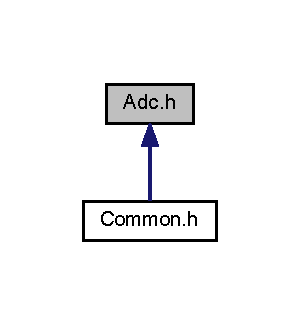
\includegraphics[width=144pt]{a00043}
\end{center}
\end{figure}
\subsection*{Functions}
\begin{DoxyCompactItemize}
\item 
void \hyperlink{a00006_af77988a3ac7a924b75e6213631b04d46}{adc\-Soc\-Cnf} (void)
\item 
void \hyperlink{a00006_a3c614312b1f0ce65b46c4d93051de836}{adc\-Macro\-Configure} (void)
\item 
void \hyperlink{a00006_a646e6cc4558594a6fbaa10c767cc4fec}{adc\-Comp\-Configure} (void)
\item 
Uint16 \hyperlink{a00006_a7dfbe5e2625efeeb0768d42d83a71c04}{adc\-Check\-Ocp} (void)
\item 
Uint16 \hyperlink{a00006_a0ad871be22e7987be07a0f4534ef231b}{adc\-Check\-Ovp} (void)
\item 
Uint16 \hyperlink{a00006_aca1e33ca1b293964f5ce58d430e684f0}{adc\-Set\-Dac} (Uint16 chnl, float32 dac\-Lvl)
\item 
Uint16 \hyperlink{a00006_a2dcc5ee51599a4026fc672072a3f8232}{adc\-Set\-I\-Scale} (Uint16 chnl, float32 scale\-Setting)
\item 
Uint16 \hyperlink{a00006_a9c87603c2aabc17d784a9149563e71e5}{adc\-Set\-V\-Scale} (Uint16 chnl, float32 scale\-Setting)
\item 
Uint16 \hyperlink{a00006_ac5c13a2ef6c3a9f9da7bf437e0213da2}{adc\-Set\-Ocp} (Uint16 chnl, float32 ocp\-Setting)
\item 
Uint16 \hyperlink{a00006_a03e263230a1a25337050bfde1172d1a1}{adc\-Set\-Ovp} (Uint16 chnl, float32 ovp\-Setting)
\item 
Uint16 \hyperlink{a00006_a51b43d0fbadcb3b231f4fceb4c7b9d12}{adc\-Get\-Dac} (Uint16 chnl, float32 $\ast$dac\-Dest)
\item 
Uint16 \hyperlink{a00006_acbf7c83ae3b6df7b0812ef1aed2b9c96}{adc\-Get\-I\-Scale} (Uint16 chnl, float32 $\ast$scl\-Dest)
\item 
Uint16 \hyperlink{a00006_a478f6261679944822575231af3eb229c}{adc\-Get\-V\-Scale} (Uint16 chnl, float32 $\ast$scl\-Dest)
\item 
Uint16 \hyperlink{a00006_a47082a746494c4221df1cb453fa746f7}{adc\-Get\-Voltage} (Uint16 chnl, float32 $\ast$v\-Dest)
\item 
Uint16 \hyperlink{a00006_a2cda2df7670a029f25848b9fe6f37bf8}{adc\-Get\-Current} (Uint16 chnl, float32 $\ast$i\-Dest)
\item 
Uint16 \hyperlink{a00006_a8e08c745a25782602c5d337d5eb7b03c}{adc\-Get\-Ocp} (Uint16 chnl, float32 $\ast$ocp\-Dest)
\item 
Uint16 \hyperlink{a00006_a1536739f53a776036e1b9c92990a102a}{adc\-Get\-Ovp} (Uint16 chnl, float32 $\ast$ovp\-Dest)
\end{DoxyCompactItemize}
\subsection*{Variables}
\begin{DoxyCompactItemize}
\item 
volatile int32 $\ast$ \hyperlink{a00006_a42ca9720519e1d0cb7ded4f56da083ba}{A\-D\-C\-D\-R\-V\-\_\-1ch\-\_\-\-Rlt1}
\item 
volatile int32 $\ast$ \hyperlink{a00006_a1ca55c7841c3e4bc154789647a068810}{A\-D\-C\-D\-R\-V\-\_\-1ch\-\_\-\-Rlt2}
\item 
volatile int32 $\ast$ \hyperlink{a00006_a1704632b071d0fff6bdc9629549c5d08}{A\-D\-C\-D\-R\-V\-\_\-1ch\-\_\-\-Rlt3}
\item 
volatile int32 $\ast$ \hyperlink{a00006_ac181cb2fb372cceb0f55844ed941c5d0}{A\-D\-C\-D\-R\-V\-\_\-1ch\-\_\-\-Rlt4}
\item 
volatile int32 $\ast$ \hyperlink{a00006_a7b586f409f6daf8232917fbd976532a4}{A\-D\-C\-D\-R\-V\-\_\-1ch\-\_\-\-Rlt5}
\item 
volatile int32 $\ast$ \hyperlink{a00006_ae8182c9b35af2d72b1c18ea41ccece2d}{A\-D\-C\-D\-R\-V\-\_\-1ch\-\_\-\-Rlt6}
\item 
volatile int32 $\ast$ \hyperlink{a00006_a4fa6265d0bf9b69d560d8f9f488b98c1}{A\-D\-C\-D\-R\-V\-\_\-1ch\-\_\-\-Rlt7}
\item 
volatile int32 $\ast$ \hyperlink{a00006_a0415309d16a115f0116a26aeda91aabd}{A\-D\-C\-D\-R\-V\-\_\-1ch\-\_\-\-Rlt8}
\item 
volatile int32 $\ast$ \hyperlink{a00006_adea6b0b8533e0d56a5c6cbac1c1e705f}{A\-D\-C\-D\-R\-V\-\_\-1ch\-\_\-\-Rlt9}
\item 
volatile int32 $\ast$ \hyperlink{a00006_ad1b851523cd317f0910f2db4220f32da}{A\-D\-C\-D\-R\-V\-\_\-1ch\-\_\-\-Rlt10}
\item 
volatile int32 $\ast$ \hyperlink{a00006_ad4435404e2f432a8c3a449dd23cda8f0}{A\-D\-C\-D\-R\-V\-\_\-1ch\-\_\-\-Rlt11}
\item 
volatile int32 $\ast$ \hyperlink{a00006_ac3656f047361723ec883e6ebfe3f026a}{A\-D\-C\-D\-R\-V\-\_\-1ch\-\_\-\-Rlt12}
\item 
volatile int32 $\ast$ \hyperlink{a00006_ad7ef0544a173d3c7883f0e739b7d2096}{A\-D\-C\-D\-R\-V\-\_\-1ch\-\_\-\-Rlt13}
\end{DoxyCompactItemize}


\subsection{Detailed Description}
A\-D\-C, D\-A\-C, comparator and related functions. Requires the modification of the C\-O\-M\-P\-\_\-\-R\-E\-G\-S struct of the D\-S\-P2802x\-\_\-\-Global\-Variable\-Defs in the file D\-S\-P2802x\-\_\-\-Comp.\-h, to allow use of the D\-A\-C\-C\-T\-L and ramp-\/related register unions. Use the equivalent file from the f2903x includes for reference. 

\subsection{Function Documentation}
\hypertarget{a00006_a7dfbe5e2625efeeb0768d42d83a71c04}{\index{Adc.\-h@{Adc.\-h}!adc\-Check\-Ocp@{adc\-Check\-Ocp}}
\index{adc\-Check\-Ocp@{adc\-Check\-Ocp}!Adc.h@{Adc.\-h}}
\subsubsection[{adc\-Check\-Ocp}]{\setlength{\rightskip}{0pt plus 5cm}Uint16 adc\-Check\-Ocp (
\begin{DoxyParamCaption}
\item[{void}]{}
\end{DoxyParamCaption}
)}}\label{a00006_a7dfbe5e2625efeeb0768d42d83a71c04}
Checks the current current sense A\-D\-C readings against the O\-C\-P limits. \begin{DoxyReturn}{Returns}
Error status 
\end{DoxyReturn}
\hypertarget{a00006_a0ad871be22e7987be07a0f4534ef231b}{\index{Adc.\-h@{Adc.\-h}!adc\-Check\-Ovp@{adc\-Check\-Ovp}}
\index{adc\-Check\-Ovp@{adc\-Check\-Ovp}!Adc.h@{Adc.\-h}}
\subsubsection[{adc\-Check\-Ovp}]{\setlength{\rightskip}{0pt plus 5cm}Uint16 adc\-Check\-Ovp (
\begin{DoxyParamCaption}
\item[{void}]{}
\end{DoxyParamCaption}
)}}\label{a00006_a0ad871be22e7987be07a0f4534ef231b}
Checks the current voltage sense A\-D\-C readings against the O\-V\-P limits. \begin{DoxyReturn}{Returns}
Error status 
\end{DoxyReturn}
\hypertarget{a00006_a646e6cc4558594a6fbaa10c767cc4fec}{\index{Adc.\-h@{Adc.\-h}!adc\-Comp\-Configure@{adc\-Comp\-Configure}}
\index{adc\-Comp\-Configure@{adc\-Comp\-Configure}!Adc.h@{Adc.\-h}}
\subsubsection[{adc\-Comp\-Configure}]{\setlength{\rightskip}{0pt plus 5cm}void adc\-Comp\-Configure (
\begin{DoxyParamCaption}
\item[{void}]{}
\end{DoxyParamCaption}
)}}\label{a00006_a646e6cc4558594a6fbaa10c767cc4fec}
Configures the C\-O\-M\-P 1 \& 2 comparators using the internal D\-A\-Cs at inverting inputs.
\begin{DoxyItemize}
\item S\-H\-O\-U\-L\-D be called A\-F\-T\-E\-R \hyperlink{a00006_af77988a3ac7a924b75e6213631b04d46}{adc\-Soc\-Cnf()}.
\item S\-H\-O\-U\-L\-D be called B\-E\-F\-O\-R\-E P\-W\-M\-S (S\-Y\-N\-C) are started.
\item S\-H\-O\-U\-L\-D be called B\-E\-F\-O\-R\-E pwm\-T\-Z\-Configure(). 
\end{DoxyItemize}\hypertarget{a00006_a2cda2df7670a029f25848b9fe6f37bf8}{\index{Adc.\-h@{Adc.\-h}!adc\-Get\-Current@{adc\-Get\-Current}}
\index{adc\-Get\-Current@{adc\-Get\-Current}!Adc.h@{Adc.\-h}}
\subsubsection[{adc\-Get\-Current}]{\setlength{\rightskip}{0pt plus 5cm}Uint16 adc\-Get\-Current (
\begin{DoxyParamCaption}
\item[{Uint16}]{chnl, }
\item[{float32 $\ast$}]{i\-Dest}
\end{DoxyParamCaption}
)}}\label{a00006_a2cda2df7670a029f25848b9fe6f37bf8}
Queries the most recent current reading from the specified channel's associated A\-D\-C. 
\begin{DoxyParams}[1]{Parameters}
\mbox{\tt in}  & {\em chnl} & Specifies the channel number on which the reading is to be queried. \\
\hline
\mbox{\tt out}  & {\em i\-Dest} & Address of the memory location at which to place the query result (amps). \\
\hline
\end{DoxyParams}
\begin{DoxyReturn}{Returns}
Error status. 
\end{DoxyReturn}
\hypertarget{a00006_a51b43d0fbadcb3b231f4fceb4c7b9d12}{\index{Adc.\-h@{Adc.\-h}!adc\-Get\-Dac@{adc\-Get\-Dac}}
\index{adc\-Get\-Dac@{adc\-Get\-Dac}!Adc.h@{Adc.\-h}}
\subsubsection[{adc\-Get\-Dac}]{\setlength{\rightskip}{0pt plus 5cm}Uint16 adc\-Get\-Dac (
\begin{DoxyParamCaption}
\item[{Uint16}]{chnl, }
\item[{float32 $\ast$}]{dac\-Dest}
\end{DoxyParamCaption}
)}}\label{a00006_a51b43d0fbadcb3b231f4fceb4c7b9d12}
Queries the output level setting of the D\-A\-C on the inverting input of the comparators. 
\begin{DoxyParams}[1]{Parameters}
\mbox{\tt in}  & {\em chnl} & Specifies the channel number on which the setting is to be queried. \\
\hline
\mbox{\tt out}  & {\em dac\-Dest} & Address of the memory location at which to place the query result (volts or amps). \\
\hline
\end{DoxyParams}
\begin{DoxyReturn}{Returns}
Error status. 
\end{DoxyReturn}
\hypertarget{a00006_acbf7c83ae3b6df7b0812ef1aed2b9c96}{\index{Adc.\-h@{Adc.\-h}!adc\-Get\-I\-Scale@{adc\-Get\-I\-Scale}}
\index{adc\-Get\-I\-Scale@{adc\-Get\-I\-Scale}!Adc.h@{Adc.\-h}}
\subsubsection[{adc\-Get\-I\-Scale}]{\setlength{\rightskip}{0pt plus 5cm}Uint16 adc\-Get\-I\-Scale (
\begin{DoxyParamCaption}
\item[{Uint16}]{chnl, }
\item[{float32 $\ast$}]{scl\-Dest}
\end{DoxyParamCaption}
)}}\label{a00006_acbf7c83ae3b6df7b0812ef1aed2b9c96}
Queries the current current scaling setting of the specified channel. 
\begin{DoxyParams}[1]{Parameters}
\mbox{\tt in}  & {\em chnl} & Specifies the channel number on which the setting is to be queried. \\
\hline
\mbox{\tt out}  & {\em scl\-Dest} & Address of the memory location at which to place the query result (amps). \\
\hline
\end{DoxyParams}
\begin{DoxyReturn}{Returns}
Error status. 
\end{DoxyReturn}
\hypertarget{a00006_a8e08c745a25782602c5d337d5eb7b03c}{\index{Adc.\-h@{Adc.\-h}!adc\-Get\-Ocp@{adc\-Get\-Ocp}}
\index{adc\-Get\-Ocp@{adc\-Get\-Ocp}!Adc.h@{Adc.\-h}}
\subsubsection[{adc\-Get\-Ocp}]{\setlength{\rightskip}{0pt plus 5cm}Uint16 adc\-Get\-Ocp (
\begin{DoxyParamCaption}
\item[{Uint16}]{chnl, }
\item[{float32 $\ast$}]{ocp\-Dest}
\end{DoxyParamCaption}
)}}\label{a00006_a8e08c745a25782602c5d337d5eb7b03c}
Queries the over current protection setting for the specified channel. 
\begin{DoxyParams}[1]{Parameters}
\mbox{\tt in}  & {\em chnl} & Specifies the channel number on which the setting is to be queried. \\
\hline
\mbox{\tt out}  & {\em ocp\-Dest} & Address of the memory location at which to place the query result (amps). \\
\hline
\end{DoxyParams}
\begin{DoxyReturn}{Returns}
Error status. 
\end{DoxyReturn}
\hypertarget{a00006_a1536739f53a776036e1b9c92990a102a}{\index{Adc.\-h@{Adc.\-h}!adc\-Get\-Ovp@{adc\-Get\-Ovp}}
\index{adc\-Get\-Ovp@{adc\-Get\-Ovp}!Adc.h@{Adc.\-h}}
\subsubsection[{adc\-Get\-Ovp}]{\setlength{\rightskip}{0pt plus 5cm}Uint16 adc\-Get\-Ovp (
\begin{DoxyParamCaption}
\item[{Uint16}]{chnl, }
\item[{float32 $\ast$}]{ovp\-Dest}
\end{DoxyParamCaption}
)}}\label{a00006_a1536739f53a776036e1b9c92990a102a}
Queries the over current protection setting for the specified channel. 
\begin{DoxyParams}[1]{Parameters}
\mbox{\tt in}  & {\em chnl} & Specifies the channel number on which the setting is to be queried. \\
\hline
\mbox{\tt out}  & {\em ovp\-Dest} & Address of the memory location at which to place the query result (volts). \\
\hline
\end{DoxyParams}
\begin{DoxyReturn}{Returns}
Error status. 
\end{DoxyReturn}
\hypertarget{a00006_a47082a746494c4221df1cb453fa746f7}{\index{Adc.\-h@{Adc.\-h}!adc\-Get\-Voltage@{adc\-Get\-Voltage}}
\index{adc\-Get\-Voltage@{adc\-Get\-Voltage}!Adc.h@{Adc.\-h}}
\subsubsection[{adc\-Get\-Voltage}]{\setlength{\rightskip}{0pt plus 5cm}Uint16 adc\-Get\-Voltage (
\begin{DoxyParamCaption}
\item[{Uint16}]{chnl, }
\item[{float32 $\ast$}]{v\-Dest}
\end{DoxyParamCaption}
)}}\label{a00006_a47082a746494c4221df1cb453fa746f7}
Queries the most recent voltage reading from the specified channel's associated A\-D\-C. 
\begin{DoxyParams}[1]{Parameters}
\mbox{\tt in}  & {\em chnl} & Specifies the channel number on which the reading is to be queried. \\
\hline
\mbox{\tt out}  & {\em v\-Dest} & Address of the memory location at which to place the query result (volts). \\
\hline
\end{DoxyParams}
\begin{DoxyReturn}{Returns}
Error status. 
\end{DoxyReturn}
\hypertarget{a00006_a478f6261679944822575231af3eb229c}{\index{Adc.\-h@{Adc.\-h}!adc\-Get\-V\-Scale@{adc\-Get\-V\-Scale}}
\index{adc\-Get\-V\-Scale@{adc\-Get\-V\-Scale}!Adc.h@{Adc.\-h}}
\subsubsection[{adc\-Get\-V\-Scale}]{\setlength{\rightskip}{0pt plus 5cm}Uint16 adc\-Get\-V\-Scale (
\begin{DoxyParamCaption}
\item[{Uint16}]{chnl, }
\item[{float32 $\ast$}]{scl\-Dest}
\end{DoxyParamCaption}
)}}\label{a00006_a478f6261679944822575231af3eb229c}
Queries the current voltage scaling setting of the specified channel. 
\begin{DoxyParams}[1]{Parameters}
\mbox{\tt in}  & {\em chnl} & Specifies the channel number on which the setting is to be queried. \\
\hline
\mbox{\tt out}  & {\em scl\-Dest} & Address of the memory location at which to place the query result (volts). \\
\hline
\end{DoxyParams}
\begin{DoxyReturn}{Returns}
Error status. 
\end{DoxyReturn}
\hypertarget{a00006_a3c614312b1f0ce65b46c4d93051de836}{\index{Adc.\-h@{Adc.\-h}!adc\-Macro\-Configure@{adc\-Macro\-Configure}}
\index{adc\-Macro\-Configure@{adc\-Macro\-Configure}!Adc.h@{Adc.\-h}}
\subsubsection[{adc\-Macro\-Configure}]{\setlength{\rightskip}{0pt plus 5cm}void adc\-Macro\-Configure (
\begin{DoxyParamCaption}
\item[{void}]{}
\end{DoxyParamCaption}
)}}\label{a00006_a3c614312b1f0ce65b46c4d93051de836}
Configures the A\-D\-C's S\-O\-Cs then calls \hyperlink{a00026_a358d8706acd0faf4e1cc705129be6548}{pwm\-Soc\-Configure()}.
\begin{DoxyItemize}
\item S\-H\-O\-U\-L\-D be run after \hyperlink{a00026_acc68120fcdfa36145370c31a61eb23a7}{pwm\-Macro\-Configure()}.
\item S\-H\-O\-U\-L\-D be run before D\-P\-L\-\_\-\-I\-N\-I\-T(). 
\end{DoxyItemize}\hypertarget{a00006_aca1e33ca1b293964f5ce58d430e684f0}{\index{Adc.\-h@{Adc.\-h}!adc\-Set\-Dac@{adc\-Set\-Dac}}
\index{adc\-Set\-Dac@{adc\-Set\-Dac}!Adc.h@{Adc.\-h}}
\subsubsection[{adc\-Set\-Dac}]{\setlength{\rightskip}{0pt plus 5cm}Uint16 adc\-Set\-Dac (
\begin{DoxyParamCaption}
\item[{Uint16}]{chnl, }
\item[{float32}]{dac\-Lvl}
\end{DoxyParamCaption}
)}}\label{a00006_aca1e33ca1b293964f5ce58d430e684f0}
Sets the output levels of the D\-A\-Cs on the inverting input of the comparators. The function will determine the scaling to be applied by testing the ctrl\-Mode setting of the channel specified. The respective channel's current or voltage M\-U\-S\-T be set previously. 
\begin{DoxyParams}[1]{Parameters}
\mbox{\tt in}  & {\em chnl} & Specifies the channel number the setting is to be applied to. \\
\hline
\mbox{\tt in}  & {\em dac\-Lvl} & Specifies the value of the level setting to be applied (volts or amps). \\
\hline
\end{DoxyParams}
\begin{DoxyReturn}{Returns}
Error status. 
\end{DoxyReturn}
\hypertarget{a00006_a2dcc5ee51599a4026fc672072a3f8232}{\index{Adc.\-h@{Adc.\-h}!adc\-Set\-I\-Scale@{adc\-Set\-I\-Scale}}
\index{adc\-Set\-I\-Scale@{adc\-Set\-I\-Scale}!Adc.h@{Adc.\-h}}
\subsubsection[{adc\-Set\-I\-Scale}]{\setlength{\rightskip}{0pt plus 5cm}Uint16 adc\-Set\-I\-Scale (
\begin{DoxyParamCaption}
\item[{Uint16}]{chnl, }
\item[{float32}]{scale\-Setting}
\end{DoxyParamCaption}
)}}\label{a00006_a2dcc5ee51599a4026fc672072a3f8232}
Sets the current scaling for the specified channel. 
\begin{DoxyParams}[1]{Parameters}
\mbox{\tt in}  & {\em chnl} & Specifies the channel number the setting is to be applied to. \\
\hline
\mbox{\tt in}  & {\em scale\-Setting} & Specifies the value of the scaling setting to be applied (amps/volts). \\
\hline
\end{DoxyParams}
\begin{DoxyReturn}{Returns}
Error status. 
\end{DoxyReturn}
\hypertarget{a00006_ac5c13a2ef6c3a9f9da7bf437e0213da2}{\index{Adc.\-h@{Adc.\-h}!adc\-Set\-Ocp@{adc\-Set\-Ocp}}
\index{adc\-Set\-Ocp@{adc\-Set\-Ocp}!Adc.h@{Adc.\-h}}
\subsubsection[{adc\-Set\-Ocp}]{\setlength{\rightskip}{0pt plus 5cm}Uint16 adc\-Set\-Ocp (
\begin{DoxyParamCaption}
\item[{Uint16}]{chnl, }
\item[{float32}]{ocp\-Setting}
\end{DoxyParamCaption}
)}}\label{a00006_ac5c13a2ef6c3a9f9da7bf437e0213da2}
Sets the over current protection limit for the specified channel. 
\begin{DoxyParams}[1]{Parameters}
\mbox{\tt in}  & {\em chnl} & Specifies the channel number the setting is to be applied to. \\
\hline
\mbox{\tt in}  & {\em ocp\-Setting} & Specifies the value of the limit to be applied (Amps). \\
\hline
\end{DoxyParams}
\begin{DoxyReturn}{Returns}
Error status. 
\end{DoxyReturn}
\hypertarget{a00006_a03e263230a1a25337050bfde1172d1a1}{\index{Adc.\-h@{Adc.\-h}!adc\-Set\-Ovp@{adc\-Set\-Ovp}}
\index{adc\-Set\-Ovp@{adc\-Set\-Ovp}!Adc.h@{Adc.\-h}}
\subsubsection[{adc\-Set\-Ovp}]{\setlength{\rightskip}{0pt plus 5cm}Uint16 adc\-Set\-Ovp (
\begin{DoxyParamCaption}
\item[{Uint16}]{chnl, }
\item[{float32}]{ovp\-Setting}
\end{DoxyParamCaption}
)}}\label{a00006_a03e263230a1a25337050bfde1172d1a1}
Sets the over voltage protection limit for the specified channel. 
\begin{DoxyParams}[1]{Parameters}
\mbox{\tt in}  & {\em chnl} & Specifies the channel number the setting is to be applied to. \\
\hline
\mbox{\tt in}  & {\em ovp\-Setting} & Specifies the value of the limit to be applied (volts). \\
\hline
\end{DoxyParams}
\begin{DoxyReturn}{Returns}
Error status. 
\end{DoxyReturn}
\hypertarget{a00006_a9c87603c2aabc17d784a9149563e71e5}{\index{Adc.\-h@{Adc.\-h}!adc\-Set\-V\-Scale@{adc\-Set\-V\-Scale}}
\index{adc\-Set\-V\-Scale@{adc\-Set\-V\-Scale}!Adc.h@{Adc.\-h}}
\subsubsection[{adc\-Set\-V\-Scale}]{\setlength{\rightskip}{0pt plus 5cm}Uint16 adc\-Set\-V\-Scale (
\begin{DoxyParamCaption}
\item[{Uint16}]{chnl, }
\item[{float32}]{scale\-Setting}
\end{DoxyParamCaption}
)}}\label{a00006_a9c87603c2aabc17d784a9149563e71e5}
Sets the voltage scaling for the specified channel. 
\begin{DoxyParams}[1]{Parameters}
\mbox{\tt in}  & {\em chnl} & Specifies the channel number the setting is to be applied to. \\
\hline
\mbox{\tt in}  & {\em scale\-Setting} & Specifies the value of the scaling setting to be applied (volts/volts). \\
\hline
\end{DoxyParams}
\begin{DoxyReturn}{Returns}
Error status. 
\end{DoxyReturn}
\hypertarget{a00006_af77988a3ac7a924b75e6213631b04d46}{\index{Adc.\-h@{Adc.\-h}!adc\-Soc\-Cnf@{adc\-Soc\-Cnf}}
\index{adc\-Soc\-Cnf@{adc\-Soc\-Cnf}!Adc.h@{Adc.\-h}}
\subsubsection[{adc\-Soc\-Cnf}]{\setlength{\rightskip}{0pt plus 5cm}void adc\-Soc\-Cnf (
\begin{DoxyParamCaption}
\item[{void}]{}
\end{DoxyParamCaption}
)}}\label{a00006_af77988a3ac7a924b75e6213631b04d46}
Configures A\-D\-C S\-O\-C for A\-D\-C macro 

\subsection{Variable Documentation}
\hypertarget{a00006_a42ca9720519e1d0cb7ded4f56da083ba}{\index{Adc.\-h@{Adc.\-h}!A\-D\-C\-D\-R\-V\-\_\-1ch\-\_\-\-Rlt1@{A\-D\-C\-D\-R\-V\-\_\-1ch\-\_\-\-Rlt1}}
\index{A\-D\-C\-D\-R\-V\-\_\-1ch\-\_\-\-Rlt1@{A\-D\-C\-D\-R\-V\-\_\-1ch\-\_\-\-Rlt1}!Adc.h@{Adc.\-h}}
\subsubsection[{A\-D\-C\-D\-R\-V\-\_\-1ch\-\_\-\-Rlt1}]{\setlength{\rightskip}{0pt plus 5cm}volatile int32$\ast$ A\-D\-C\-D\-R\-V\-\_\-1ch\-\_\-\-Rlt1}}\label{a00006_a42ca9720519e1d0cb7ded4f56da083ba}
Channel 0 current sense A\-D\-C terminal pointer. \hypertarget{a00006_ad1b851523cd317f0910f2db4220f32da}{\index{Adc.\-h@{Adc.\-h}!A\-D\-C\-D\-R\-V\-\_\-1ch\-\_\-\-Rlt10@{A\-D\-C\-D\-R\-V\-\_\-1ch\-\_\-\-Rlt10}}
\index{A\-D\-C\-D\-R\-V\-\_\-1ch\-\_\-\-Rlt10@{A\-D\-C\-D\-R\-V\-\_\-1ch\-\_\-\-Rlt10}!Adc.h@{Adc.\-h}}
\subsubsection[{A\-D\-C\-D\-R\-V\-\_\-1ch\-\_\-\-Rlt10}]{\setlength{\rightskip}{0pt plus 5cm}volatile int32$\ast$ A\-D\-C\-D\-R\-V\-\_\-1ch\-\_\-\-Rlt10}}\label{a00006_ad1b851523cd317f0910f2db4220f32da}
Channel 3 voltage sense A\-D\-C terminal pointer. \hypertarget{a00006_ad4435404e2f432a8c3a449dd23cda8f0}{\index{Adc.\-h@{Adc.\-h}!A\-D\-C\-D\-R\-V\-\_\-1ch\-\_\-\-Rlt11@{A\-D\-C\-D\-R\-V\-\_\-1ch\-\_\-\-Rlt11}}
\index{A\-D\-C\-D\-R\-V\-\_\-1ch\-\_\-\-Rlt11@{A\-D\-C\-D\-R\-V\-\_\-1ch\-\_\-\-Rlt11}!Adc.h@{Adc.\-h}}
\subsubsection[{A\-D\-C\-D\-R\-V\-\_\-1ch\-\_\-\-Rlt11}]{\setlength{\rightskip}{0pt plus 5cm}volatile int32$\ast$ A\-D\-C\-D\-R\-V\-\_\-1ch\-\_\-\-Rlt11}}\label{a00006_ad4435404e2f432a8c3a449dd23cda8f0}
Interboost voltage sense A\-D\-C terminal pointer. \hypertarget{a00006_ac3656f047361723ec883e6ebfe3f026a}{\index{Adc.\-h@{Adc.\-h}!A\-D\-C\-D\-R\-V\-\_\-1ch\-\_\-\-Rlt12@{A\-D\-C\-D\-R\-V\-\_\-1ch\-\_\-\-Rlt12}}
\index{A\-D\-C\-D\-R\-V\-\_\-1ch\-\_\-\-Rlt12@{A\-D\-C\-D\-R\-V\-\_\-1ch\-\_\-\-Rlt12}!Adc.h@{Adc.\-h}}
\subsubsection[{A\-D\-C\-D\-R\-V\-\_\-1ch\-\_\-\-Rlt12}]{\setlength{\rightskip}{0pt plus 5cm}volatile int32$\ast$ A\-D\-C\-D\-R\-V\-\_\-1ch\-\_\-\-Rlt12}}\label{a00006_ac3656f047361723ec883e6ebfe3f026a}
A\-C stage voltage sense A\-D\-C terminal pointer. \hypertarget{a00006_ad7ef0544a173d3c7883f0e739b7d2096}{\index{Adc.\-h@{Adc.\-h}!A\-D\-C\-D\-R\-V\-\_\-1ch\-\_\-\-Rlt13@{A\-D\-C\-D\-R\-V\-\_\-1ch\-\_\-\-Rlt13}}
\index{A\-D\-C\-D\-R\-V\-\_\-1ch\-\_\-\-Rlt13@{A\-D\-C\-D\-R\-V\-\_\-1ch\-\_\-\-Rlt13}!Adc.h@{Adc.\-h}}
\subsubsection[{A\-D\-C\-D\-R\-V\-\_\-1ch\-\_\-\-Rlt13}]{\setlength{\rightskip}{0pt plus 5cm}volatile int32$\ast$ A\-D\-C\-D\-R\-V\-\_\-1ch\-\_\-\-Rlt13}}\label{a00006_ad7ef0544a173d3c7883f0e739b7d2096}
V\-Mid voltage sense A\-D\-C terminal pointer. \hypertarget{a00006_a1ca55c7841c3e4bc154789647a068810}{\index{Adc.\-h@{Adc.\-h}!A\-D\-C\-D\-R\-V\-\_\-1ch\-\_\-\-Rlt2@{A\-D\-C\-D\-R\-V\-\_\-1ch\-\_\-\-Rlt2}}
\index{A\-D\-C\-D\-R\-V\-\_\-1ch\-\_\-\-Rlt2@{A\-D\-C\-D\-R\-V\-\_\-1ch\-\_\-\-Rlt2}!Adc.h@{Adc.\-h}}
\subsubsection[{A\-D\-C\-D\-R\-V\-\_\-1ch\-\_\-\-Rlt2}]{\setlength{\rightskip}{0pt plus 5cm}volatile int32$\ast$ A\-D\-C\-D\-R\-V\-\_\-1ch\-\_\-\-Rlt2}}\label{a00006_a1ca55c7841c3e4bc154789647a068810}
Channel 1 current sense A\-D\-C terminal pointer. \hypertarget{a00006_a1704632b071d0fff6bdc9629549c5d08}{\index{Adc.\-h@{Adc.\-h}!A\-D\-C\-D\-R\-V\-\_\-1ch\-\_\-\-Rlt3@{A\-D\-C\-D\-R\-V\-\_\-1ch\-\_\-\-Rlt3}}
\index{A\-D\-C\-D\-R\-V\-\_\-1ch\-\_\-\-Rlt3@{A\-D\-C\-D\-R\-V\-\_\-1ch\-\_\-\-Rlt3}!Adc.h@{Adc.\-h}}
\subsubsection[{A\-D\-C\-D\-R\-V\-\_\-1ch\-\_\-\-Rlt3}]{\setlength{\rightskip}{0pt plus 5cm}volatile int32$\ast$ A\-D\-C\-D\-R\-V\-\_\-1ch\-\_\-\-Rlt3}}\label{a00006_a1704632b071d0fff6bdc9629549c5d08}
Channel 2 current sense A\-D\-C terminal pointer. \hypertarget{a00006_ac181cb2fb372cceb0f55844ed941c5d0}{\index{Adc.\-h@{Adc.\-h}!A\-D\-C\-D\-R\-V\-\_\-1ch\-\_\-\-Rlt4@{A\-D\-C\-D\-R\-V\-\_\-1ch\-\_\-\-Rlt4}}
\index{A\-D\-C\-D\-R\-V\-\_\-1ch\-\_\-\-Rlt4@{A\-D\-C\-D\-R\-V\-\_\-1ch\-\_\-\-Rlt4}!Adc.h@{Adc.\-h}}
\subsubsection[{A\-D\-C\-D\-R\-V\-\_\-1ch\-\_\-\-Rlt4}]{\setlength{\rightskip}{0pt plus 5cm}volatile int32$\ast$ A\-D\-C\-D\-R\-V\-\_\-1ch\-\_\-\-Rlt4}}\label{a00006_ac181cb2fb372cceb0f55844ed941c5d0}
Channel 3 current sense A\-D\-C terminal pointer. \hypertarget{a00006_a7b586f409f6daf8232917fbd976532a4}{\index{Adc.\-h@{Adc.\-h}!A\-D\-C\-D\-R\-V\-\_\-1ch\-\_\-\-Rlt5@{A\-D\-C\-D\-R\-V\-\_\-1ch\-\_\-\-Rlt5}}
\index{A\-D\-C\-D\-R\-V\-\_\-1ch\-\_\-\-Rlt5@{A\-D\-C\-D\-R\-V\-\_\-1ch\-\_\-\-Rlt5}!Adc.h@{Adc.\-h}}
\subsubsection[{A\-D\-C\-D\-R\-V\-\_\-1ch\-\_\-\-Rlt5}]{\setlength{\rightskip}{0pt plus 5cm}volatile int32$\ast$ A\-D\-C\-D\-R\-V\-\_\-1ch\-\_\-\-Rlt5}}\label{a00006_a7b586f409f6daf8232917fbd976532a4}
Interboost current sense A\-D\-C terminal pointer. \hypertarget{a00006_ae8182c9b35af2d72b1c18ea41ccece2d}{\index{Adc.\-h@{Adc.\-h}!A\-D\-C\-D\-R\-V\-\_\-1ch\-\_\-\-Rlt6@{A\-D\-C\-D\-R\-V\-\_\-1ch\-\_\-\-Rlt6}}
\index{A\-D\-C\-D\-R\-V\-\_\-1ch\-\_\-\-Rlt6@{A\-D\-C\-D\-R\-V\-\_\-1ch\-\_\-\-Rlt6}!Adc.h@{Adc.\-h}}
\subsubsection[{A\-D\-C\-D\-R\-V\-\_\-1ch\-\_\-\-Rlt6}]{\setlength{\rightskip}{0pt plus 5cm}volatile int32$\ast$ A\-D\-C\-D\-R\-V\-\_\-1ch\-\_\-\-Rlt6}}\label{a00006_ae8182c9b35af2d72b1c18ea41ccece2d}
A\-C stage current sense A\-D\-C terminal pointer. \hypertarget{a00006_a4fa6265d0bf9b69d560d8f9f488b98c1}{\index{Adc.\-h@{Adc.\-h}!A\-D\-C\-D\-R\-V\-\_\-1ch\-\_\-\-Rlt7@{A\-D\-C\-D\-R\-V\-\_\-1ch\-\_\-\-Rlt7}}
\index{A\-D\-C\-D\-R\-V\-\_\-1ch\-\_\-\-Rlt7@{A\-D\-C\-D\-R\-V\-\_\-1ch\-\_\-\-Rlt7}!Adc.h@{Adc.\-h}}
\subsubsection[{A\-D\-C\-D\-R\-V\-\_\-1ch\-\_\-\-Rlt7}]{\setlength{\rightskip}{0pt plus 5cm}volatile int32$\ast$ A\-D\-C\-D\-R\-V\-\_\-1ch\-\_\-\-Rlt7}}\label{a00006_a4fa6265d0bf9b69d560d8f9f488b98c1}
Channel 0 voltage sense A\-D\-C terminal pointer. \hypertarget{a00006_a0415309d16a115f0116a26aeda91aabd}{\index{Adc.\-h@{Adc.\-h}!A\-D\-C\-D\-R\-V\-\_\-1ch\-\_\-\-Rlt8@{A\-D\-C\-D\-R\-V\-\_\-1ch\-\_\-\-Rlt8}}
\index{A\-D\-C\-D\-R\-V\-\_\-1ch\-\_\-\-Rlt8@{A\-D\-C\-D\-R\-V\-\_\-1ch\-\_\-\-Rlt8}!Adc.h@{Adc.\-h}}
\subsubsection[{A\-D\-C\-D\-R\-V\-\_\-1ch\-\_\-\-Rlt8}]{\setlength{\rightskip}{0pt plus 5cm}volatile int32$\ast$ A\-D\-C\-D\-R\-V\-\_\-1ch\-\_\-\-Rlt8}}\label{a00006_a0415309d16a115f0116a26aeda91aabd}
Channel 1 voltage sense A\-D\-C terminal pointer. \hypertarget{a00006_adea6b0b8533e0d56a5c6cbac1c1e705f}{\index{Adc.\-h@{Adc.\-h}!A\-D\-C\-D\-R\-V\-\_\-1ch\-\_\-\-Rlt9@{A\-D\-C\-D\-R\-V\-\_\-1ch\-\_\-\-Rlt9}}
\index{A\-D\-C\-D\-R\-V\-\_\-1ch\-\_\-\-Rlt9@{A\-D\-C\-D\-R\-V\-\_\-1ch\-\_\-\-Rlt9}!Adc.h@{Adc.\-h}}
\subsubsection[{A\-D\-C\-D\-R\-V\-\_\-1ch\-\_\-\-Rlt9}]{\setlength{\rightskip}{0pt plus 5cm}volatile int32$\ast$ A\-D\-C\-D\-R\-V\-\_\-1ch\-\_\-\-Rlt9}}\label{a00006_adea6b0b8533e0d56a5c6cbac1c1e705f}
Channel 2 voltage sense A\-D\-C terminal pointer. 
\hypertarget{a00007}{\section{Bst\-En.\-h File Reference}
\label{a00007}\index{Bst\-En.\-h@{Bst\-En.\-h}}
}


Functions for enabling and disabling the boost converter stages via I2\-C.  


This graph shows which files directly or indirectly include this file\-:\nopagebreak
\begin{figure}[H]
\begin{center}
\leavevmode
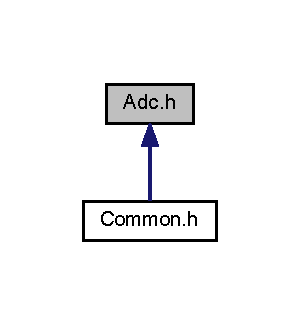
\includegraphics[width=144pt]{a00043}
\end{center}
\end{figure}
\subsection*{Macros}
\begin{DoxyCompactItemize}
\item 
\#define \hyperlink{a00007_ad615a329bea187ce779cf9930ba8a6fa}{I\-O\-E\-\_\-\-I2\-C\-\_\-\-A\-D\-D\-R}~0x20
\item 
\#define \hyperlink{a00007_a36c134b088cc2e64e0a5e14e8f90fe38}{I\-O\-E\-\_\-\-I\-O\-D\-I\-R\-\_\-\-A\-D\-D\-R}~0x00
\item 
\#define \hyperlink{a00007_a04633cd2ea7fd0b332e1edf066f674c4}{I\-O\-E\-\_\-\-I\-P\-O\-L\-\_\-\-A\-D\-D\-R}~0x01
\item 
\#define \hyperlink{a00007_aa68be5a6ed28fb146600b4fd2d11fafd}{I\-O\-E\-\_\-\-G\-P\-I\-N\-T\-E\-N\-\_\-\-A\-D\-D\-R}~0x02
\item 
\#define \hyperlink{a00007_a687e15212e8d4b49c12159dce73eeeab}{I\-O\-E\-\_\-\-D\-E\-F\-V\-A\-L\-\_\-\-A\-D\-D\-R}~0x03
\item 
\#define \hyperlink{a00007_a90945d9544eebc892154f1e0443b1407}{I\-O\-E\-\_\-\-I\-N\-T\-C\-O\-N\-\_\-\-A\-D\-D\-R}~0x04
\item 
\#define \hyperlink{a00007_af44ed2bf93808aeb932ce9944a942b75}{I\-O\-E\-\_\-\-I\-O\-C\-O\-N\-\_\-\-A\-D\-D\-R}~0x05
\item 
\#define \hyperlink{a00007_a91e588d697383f94de2bf7f11d9ecb4b}{I\-O\-E\-\_\-\-G\-P\-P\-U\-\_\-\-A\-D\-D\-R}~0x06
\item 
\#define \hyperlink{a00007_a32cac2ad5af58a2562540ec8fc205dd1}{I\-O\-E\-\_\-\-I\-N\-T\-F\-\_\-\-A\-D\-D\-R}~0x07
\item 
\#define \hyperlink{a00007_ac0afd8503a8584599cc81f3d9b0a04dc}{I\-O\-E\-\_\-\-I\-N\-T\-C\-A\-P\-\_\-\-A\-D\-D\-R}~0x08
\item 
\#define \hyperlink{a00007_af2d85152c5775a221f107d6de547bca1}{I\-O\-E\-\_\-\-G\-P\-I\-O\-\_\-\-A\-D\-D\-R}~0x09
\item 
\#define \hyperlink{a00007_ab26864d7372ac11db9c1996842a3cf56}{I\-O\-E\-\_\-\-O\-L\-A\-T\-\_\-\-A\-D\-D\-R}~0x0\-A
\item 
\#define \hyperlink{a00007_ac36a77a8d07d8025000e3e748cea40dd}{B\-S\-T\-\_\-\-N\-U\-M\-\_\-\-C\-H\-N\-L}~0x04
\item 
\#define \hyperlink{a00007_a5b329f52cf0129bf56d1b16eb706dee4}{I\-O\-E\-\_\-\-N\-U\-M\-\_\-\-C\-H\-N\-L}~\hyperlink{a00007_ac36a77a8d07d8025000e3e748cea40dd}{B\-S\-T\-\_\-\-N\-U\-M\-\_\-\-C\-H\-N\-L}
\end{DoxyCompactItemize}
\subsection*{Functions}
\begin{DoxyCompactItemize}
\item 
Uint16 \hyperlink{a00007_aa6cb02a7aacce8671212b21ed6e39863}{bc\-Init} (void)
\item 
Uint16 \hyperlink{a00007_af10c5e095b6142ee37930042bd1da708}{bc\-Enable} (Uint16 chnl)
\item 
Uint16 \hyperlink{a00007_a3df6954c93c9089cdc750fff4b89da3e}{bc\-Disable} (Uint16 chnl)
\end{DoxyCompactItemize}


\subsection{Detailed Description}
Functions for enabling and disabling the boost converter stages via I2\-C. The converters are controlled via an external I/\-O expander (M\-C\-P23008) that is connected to the I2\-C bus at address 0100x-\/x-\/x where 'x-\/x-\/x' is dependent upon the configuration of resistors R60 -\/ 61 \& R70 -\/ R74.

After \hyperlink{a00007_aa6cb02a7aacce8671212b21ed6e39863}{bc\-Init()} all converters default to disabled.

\begin{DoxyWarning}{Warning}
Before any converter control functions can be used the I2\-C peripheral M\-U\-S\-T be initialised and E\-I\-T\-H\-E\-R \hyperlink{a00007_aa6cb02a7aacce8671212b21ed6e39863}{bc\-Init()} or \hyperlink{a00015_a3506b5e25346351ce292e2ad256607cc}{fc\-Init()} M\-U\-S\-T be run -\/ \hyperlink{a00007_aa6cb02a7aacce8671212b21ed6e39863}{bc\-Init()} will require the interrupts to be enabled globally.
\end{DoxyWarning}
\begin{DoxySeeAlso}{See Also}
\hyperlink{a00017_a1e0a81a1ad1fd7710ca189236e3e5476}{i2c\-Init()} 

\hyperlink{a00015_a3506b5e25346351ce292e2ad256607cc}{fc\-Init()} 
\end{DoxySeeAlso}


\subsection{Macro Definition Documentation}
\hypertarget{a00007_ac36a77a8d07d8025000e3e748cea40dd}{\index{Bst\-En.\-h@{Bst\-En.\-h}!B\-S\-T\-\_\-\-N\-U\-M\-\_\-\-C\-H\-N\-L@{B\-S\-T\-\_\-\-N\-U\-M\-\_\-\-C\-H\-N\-L}}
\index{B\-S\-T\-\_\-\-N\-U\-M\-\_\-\-C\-H\-N\-L@{B\-S\-T\-\_\-\-N\-U\-M\-\_\-\-C\-H\-N\-L}!BstEn.h@{Bst\-En.\-h}}
\subsubsection[{B\-S\-T\-\_\-\-N\-U\-M\-\_\-\-C\-H\-N\-L}]{\setlength{\rightskip}{0pt plus 5cm}\#define B\-S\-T\-\_\-\-N\-U\-M\-\_\-\-C\-H\-N\-L~0x04}}\label{a00007_ac36a77a8d07d8025000e3e748cea40dd}
Number of boost converter channels. \hypertarget{a00007_a687e15212e8d4b49c12159dce73eeeab}{\index{Bst\-En.\-h@{Bst\-En.\-h}!I\-O\-E\-\_\-\-D\-E\-F\-V\-A\-L\-\_\-\-A\-D\-D\-R@{I\-O\-E\-\_\-\-D\-E\-F\-V\-A\-L\-\_\-\-A\-D\-D\-R}}
\index{I\-O\-E\-\_\-\-D\-E\-F\-V\-A\-L\-\_\-\-A\-D\-D\-R@{I\-O\-E\-\_\-\-D\-E\-F\-V\-A\-L\-\_\-\-A\-D\-D\-R}!BstEn.h@{Bst\-En.\-h}}
\subsubsection[{I\-O\-E\-\_\-\-D\-E\-F\-V\-A\-L\-\_\-\-A\-D\-D\-R}]{\setlength{\rightskip}{0pt plus 5cm}\#define I\-O\-E\-\_\-\-D\-E\-F\-V\-A\-L\-\_\-\-A\-D\-D\-R~0x03}}\label{a00007_a687e15212e8d4b49c12159dce73eeeab}
M\-C\-P23008 I/\-O expander default value register address. \hypertarget{a00007_aa68be5a6ed28fb146600b4fd2d11fafd}{\index{Bst\-En.\-h@{Bst\-En.\-h}!I\-O\-E\-\_\-\-G\-P\-I\-N\-T\-E\-N\-\_\-\-A\-D\-D\-R@{I\-O\-E\-\_\-\-G\-P\-I\-N\-T\-E\-N\-\_\-\-A\-D\-D\-R}}
\index{I\-O\-E\-\_\-\-G\-P\-I\-N\-T\-E\-N\-\_\-\-A\-D\-D\-R@{I\-O\-E\-\_\-\-G\-P\-I\-N\-T\-E\-N\-\_\-\-A\-D\-D\-R}!BstEn.h@{Bst\-En.\-h}}
\subsubsection[{I\-O\-E\-\_\-\-G\-P\-I\-N\-T\-E\-N\-\_\-\-A\-D\-D\-R}]{\setlength{\rightskip}{0pt plus 5cm}\#define I\-O\-E\-\_\-\-G\-P\-I\-N\-T\-E\-N\-\_\-\-A\-D\-D\-R~0x02}}\label{a00007_aa68be5a6ed28fb146600b4fd2d11fafd}
M\-C\-P23008 I/\-O expander interrupt on change enable register address. \hypertarget{a00007_af2d85152c5775a221f107d6de547bca1}{\index{Bst\-En.\-h@{Bst\-En.\-h}!I\-O\-E\-\_\-\-G\-P\-I\-O\-\_\-\-A\-D\-D\-R@{I\-O\-E\-\_\-\-G\-P\-I\-O\-\_\-\-A\-D\-D\-R}}
\index{I\-O\-E\-\_\-\-G\-P\-I\-O\-\_\-\-A\-D\-D\-R@{I\-O\-E\-\_\-\-G\-P\-I\-O\-\_\-\-A\-D\-D\-R}!BstEn.h@{Bst\-En.\-h}}
\subsubsection[{I\-O\-E\-\_\-\-G\-P\-I\-O\-\_\-\-A\-D\-D\-R}]{\setlength{\rightskip}{0pt plus 5cm}\#define I\-O\-E\-\_\-\-G\-P\-I\-O\-\_\-\-A\-D\-D\-R~0x09}}\label{a00007_af2d85152c5775a221f107d6de547bca1}
M\-C\-P23008 I/\-O expander G\-P\-I\-O port register address. \hypertarget{a00007_a91e588d697383f94de2bf7f11d9ecb4b}{\index{Bst\-En.\-h@{Bst\-En.\-h}!I\-O\-E\-\_\-\-G\-P\-P\-U\-\_\-\-A\-D\-D\-R@{I\-O\-E\-\_\-\-G\-P\-P\-U\-\_\-\-A\-D\-D\-R}}
\index{I\-O\-E\-\_\-\-G\-P\-P\-U\-\_\-\-A\-D\-D\-R@{I\-O\-E\-\_\-\-G\-P\-P\-U\-\_\-\-A\-D\-D\-R}!BstEn.h@{Bst\-En.\-h}}
\subsubsection[{I\-O\-E\-\_\-\-G\-P\-P\-U\-\_\-\-A\-D\-D\-R}]{\setlength{\rightskip}{0pt plus 5cm}\#define I\-O\-E\-\_\-\-G\-P\-P\-U\-\_\-\-A\-D\-D\-R~0x06}}\label{a00007_a91e588d697383f94de2bf7f11d9ecb4b}
M\-C\-P23008 I/\-O expander pull-\/up resistor configuration register address. \hypertarget{a00007_ad615a329bea187ce779cf9930ba8a6fa}{\index{Bst\-En.\-h@{Bst\-En.\-h}!I\-O\-E\-\_\-\-I2\-C\-\_\-\-A\-D\-D\-R@{I\-O\-E\-\_\-\-I2\-C\-\_\-\-A\-D\-D\-R}}
\index{I\-O\-E\-\_\-\-I2\-C\-\_\-\-A\-D\-D\-R@{I\-O\-E\-\_\-\-I2\-C\-\_\-\-A\-D\-D\-R}!BstEn.h@{Bst\-En.\-h}}
\subsubsection[{I\-O\-E\-\_\-\-I2\-C\-\_\-\-A\-D\-D\-R}]{\setlength{\rightskip}{0pt plus 5cm}\#define I\-O\-E\-\_\-\-I2\-C\-\_\-\-A\-D\-D\-R~0x20}}\label{a00007_ad615a329bea187ce779cf9930ba8a6fa}
M\-C\-P23008 I/\-O expander I2\-C address (slave, 32d, 8-\/bit I/\-O expander). \hypertarget{a00007_ac0afd8503a8584599cc81f3d9b0a04dc}{\index{Bst\-En.\-h@{Bst\-En.\-h}!I\-O\-E\-\_\-\-I\-N\-T\-C\-A\-P\-\_\-\-A\-D\-D\-R@{I\-O\-E\-\_\-\-I\-N\-T\-C\-A\-P\-\_\-\-A\-D\-D\-R}}
\index{I\-O\-E\-\_\-\-I\-N\-T\-C\-A\-P\-\_\-\-A\-D\-D\-R@{I\-O\-E\-\_\-\-I\-N\-T\-C\-A\-P\-\_\-\-A\-D\-D\-R}!BstEn.h@{Bst\-En.\-h}}
\subsubsection[{I\-O\-E\-\_\-\-I\-N\-T\-C\-A\-P\-\_\-\-A\-D\-D\-R}]{\setlength{\rightskip}{0pt plus 5cm}\#define I\-O\-E\-\_\-\-I\-N\-T\-C\-A\-P\-\_\-\-A\-D\-D\-R~0x08}}\label{a00007_ac0afd8503a8584599cc81f3d9b0a04dc}
M\-C\-P23008 I/\-O expander interrupt capture register address. \hypertarget{a00007_a90945d9544eebc892154f1e0443b1407}{\index{Bst\-En.\-h@{Bst\-En.\-h}!I\-O\-E\-\_\-\-I\-N\-T\-C\-O\-N\-\_\-\-A\-D\-D\-R@{I\-O\-E\-\_\-\-I\-N\-T\-C\-O\-N\-\_\-\-A\-D\-D\-R}}
\index{I\-O\-E\-\_\-\-I\-N\-T\-C\-O\-N\-\_\-\-A\-D\-D\-R@{I\-O\-E\-\_\-\-I\-N\-T\-C\-O\-N\-\_\-\-A\-D\-D\-R}!BstEn.h@{Bst\-En.\-h}}
\subsubsection[{I\-O\-E\-\_\-\-I\-N\-T\-C\-O\-N\-\_\-\-A\-D\-D\-R}]{\setlength{\rightskip}{0pt plus 5cm}\#define I\-O\-E\-\_\-\-I\-N\-T\-C\-O\-N\-\_\-\-A\-D\-D\-R~0x04}}\label{a00007_a90945d9544eebc892154f1e0443b1407}
M\-C\-P23008 I/\-O expander interrupt on change control register address. \hypertarget{a00007_a32cac2ad5af58a2562540ec8fc205dd1}{\index{Bst\-En.\-h@{Bst\-En.\-h}!I\-O\-E\-\_\-\-I\-N\-T\-F\-\_\-\-A\-D\-D\-R@{I\-O\-E\-\_\-\-I\-N\-T\-F\-\_\-\-A\-D\-D\-R}}
\index{I\-O\-E\-\_\-\-I\-N\-T\-F\-\_\-\-A\-D\-D\-R@{I\-O\-E\-\_\-\-I\-N\-T\-F\-\_\-\-A\-D\-D\-R}!BstEn.h@{Bst\-En.\-h}}
\subsubsection[{I\-O\-E\-\_\-\-I\-N\-T\-F\-\_\-\-A\-D\-D\-R}]{\setlength{\rightskip}{0pt plus 5cm}\#define I\-O\-E\-\_\-\-I\-N\-T\-F\-\_\-\-A\-D\-D\-R~0x07}}\label{a00007_a32cac2ad5af58a2562540ec8fc205dd1}
M\-C\-P23008 I/\-O expander interrupt flag register address. \hypertarget{a00007_af44ed2bf93808aeb932ce9944a942b75}{\index{Bst\-En.\-h@{Bst\-En.\-h}!I\-O\-E\-\_\-\-I\-O\-C\-O\-N\-\_\-\-A\-D\-D\-R@{I\-O\-E\-\_\-\-I\-O\-C\-O\-N\-\_\-\-A\-D\-D\-R}}
\index{I\-O\-E\-\_\-\-I\-O\-C\-O\-N\-\_\-\-A\-D\-D\-R@{I\-O\-E\-\_\-\-I\-O\-C\-O\-N\-\_\-\-A\-D\-D\-R}!BstEn.h@{Bst\-En.\-h}}
\subsubsection[{I\-O\-E\-\_\-\-I\-O\-C\-O\-N\-\_\-\-A\-D\-D\-R}]{\setlength{\rightskip}{0pt plus 5cm}\#define I\-O\-E\-\_\-\-I\-O\-C\-O\-N\-\_\-\-A\-D\-D\-R~0x05}}\label{a00007_af44ed2bf93808aeb932ce9944a942b75}
M\-C\-P23008 I/\-O expander configuration register address. \hypertarget{a00007_a36c134b088cc2e64e0a5e14e8f90fe38}{\index{Bst\-En.\-h@{Bst\-En.\-h}!I\-O\-E\-\_\-\-I\-O\-D\-I\-R\-\_\-\-A\-D\-D\-R@{I\-O\-E\-\_\-\-I\-O\-D\-I\-R\-\_\-\-A\-D\-D\-R}}
\index{I\-O\-E\-\_\-\-I\-O\-D\-I\-R\-\_\-\-A\-D\-D\-R@{I\-O\-E\-\_\-\-I\-O\-D\-I\-R\-\_\-\-A\-D\-D\-R}!BstEn.h@{Bst\-En.\-h}}
\subsubsection[{I\-O\-E\-\_\-\-I\-O\-D\-I\-R\-\_\-\-A\-D\-D\-R}]{\setlength{\rightskip}{0pt plus 5cm}\#define I\-O\-E\-\_\-\-I\-O\-D\-I\-R\-\_\-\-A\-D\-D\-R~0x00}}\label{a00007_a36c134b088cc2e64e0a5e14e8f90fe38}
M\-C\-P23008 I/\-O expander I/\-O direction register address. \hypertarget{a00007_a04633cd2ea7fd0b332e1edf066f674c4}{\index{Bst\-En.\-h@{Bst\-En.\-h}!I\-O\-E\-\_\-\-I\-P\-O\-L\-\_\-\-A\-D\-D\-R@{I\-O\-E\-\_\-\-I\-P\-O\-L\-\_\-\-A\-D\-D\-R}}
\index{I\-O\-E\-\_\-\-I\-P\-O\-L\-\_\-\-A\-D\-D\-R@{I\-O\-E\-\_\-\-I\-P\-O\-L\-\_\-\-A\-D\-D\-R}!BstEn.h@{Bst\-En.\-h}}
\subsubsection[{I\-O\-E\-\_\-\-I\-P\-O\-L\-\_\-\-A\-D\-D\-R}]{\setlength{\rightskip}{0pt plus 5cm}\#define I\-O\-E\-\_\-\-I\-P\-O\-L\-\_\-\-A\-D\-D\-R~0x01}}\label{a00007_a04633cd2ea7fd0b332e1edf066f674c4}
M\-C\-P23008 I/\-O expander input polarity register address. \hypertarget{a00007_a5b329f52cf0129bf56d1b16eb706dee4}{\index{Bst\-En.\-h@{Bst\-En.\-h}!I\-O\-E\-\_\-\-N\-U\-M\-\_\-\-C\-H\-N\-L@{I\-O\-E\-\_\-\-N\-U\-M\-\_\-\-C\-H\-N\-L}}
\index{I\-O\-E\-\_\-\-N\-U\-M\-\_\-\-C\-H\-N\-L@{I\-O\-E\-\_\-\-N\-U\-M\-\_\-\-C\-H\-N\-L}!BstEn.h@{Bst\-En.\-h}}
\subsubsection[{I\-O\-E\-\_\-\-N\-U\-M\-\_\-\-C\-H\-N\-L}]{\setlength{\rightskip}{0pt plus 5cm}\#define I\-O\-E\-\_\-\-N\-U\-M\-\_\-\-C\-H\-N\-L~{\bf B\-S\-T\-\_\-\-N\-U\-M\-\_\-\-C\-H\-N\-L}}}\label{a00007_a5b329f52cf0129bf56d1b16eb706dee4}
Total number of M\-C\-P I/\-O expander channels. \hypertarget{a00007_ab26864d7372ac11db9c1996842a3cf56}{\index{Bst\-En.\-h@{Bst\-En.\-h}!I\-O\-E\-\_\-\-O\-L\-A\-T\-\_\-\-A\-D\-D\-R@{I\-O\-E\-\_\-\-O\-L\-A\-T\-\_\-\-A\-D\-D\-R}}
\index{I\-O\-E\-\_\-\-O\-L\-A\-T\-\_\-\-A\-D\-D\-R@{I\-O\-E\-\_\-\-O\-L\-A\-T\-\_\-\-A\-D\-D\-R}!BstEn.h@{Bst\-En.\-h}}
\subsubsection[{I\-O\-E\-\_\-\-O\-L\-A\-T\-\_\-\-A\-D\-D\-R}]{\setlength{\rightskip}{0pt plus 5cm}\#define I\-O\-E\-\_\-\-O\-L\-A\-T\-\_\-\-A\-D\-D\-R~0x0\-A}}\label{a00007_ab26864d7372ac11db9c1996842a3cf56}
M\-C\-P23008 I/\-O expander output latch register address. 

\subsection{Function Documentation}
\hypertarget{a00007_a3df6954c93c9089cdc750fff4b89da3e}{\index{Bst\-En.\-h@{Bst\-En.\-h}!bc\-Disable@{bc\-Disable}}
\index{bc\-Disable@{bc\-Disable}!BstEn.h@{Bst\-En.\-h}}
\subsubsection[{bc\-Disable}]{\setlength{\rightskip}{0pt plus 5cm}Uint16 bc\-Disable (
\begin{DoxyParamCaption}
\item[{Uint16}]{chnl}
\end{DoxyParamCaption}
)}}\label{a00007_a3df6954c93c9089cdc750fff4b89da3e}
Disables the specified channel's boost converter. The I2\-C peripheral and the boost converter enable controller interface M\-U\-S\-T be initialised before this function is used. \begin{DoxySeeAlso}{See Also}
\hyperlink{a00017_a1e0a81a1ad1fd7710ca189236e3e5476}{i2c\-Init()} 

\hyperlink{a00007_aa6cb02a7aacce8671212b21ed6e39863}{bc\-Init()} 
\end{DoxySeeAlso}

\begin{DoxyParams}[1]{Parameters}
\mbox{\tt in}  & {\em chnl} & Specifies the channel boost that is to be disabled. \\
\hline
\end{DoxyParams}
\begin{DoxyReturn}{Returns}
Error status. 
\end{DoxyReturn}
\hypertarget{a00007_af10c5e095b6142ee37930042bd1da708}{\index{Bst\-En.\-h@{Bst\-En.\-h}!bc\-Enable@{bc\-Enable}}
\index{bc\-Enable@{bc\-Enable}!BstEn.h@{Bst\-En.\-h}}
\subsubsection[{bc\-Enable}]{\setlength{\rightskip}{0pt plus 5cm}Uint16 bc\-Enable (
\begin{DoxyParamCaption}
\item[{Uint16}]{chnl}
\end{DoxyParamCaption}
)}}\label{a00007_af10c5e095b6142ee37930042bd1da708}
Enables the specified channel's boost converter. The I2\-C peripheral and the boost converter enable controller interface M\-U\-S\-T be initialised before this function is used. \begin{DoxySeeAlso}{See Also}
\hyperlink{a00017_a1e0a81a1ad1fd7710ca189236e3e5476}{i2c\-Init()} 

\hyperlink{a00007_aa6cb02a7aacce8671212b21ed6e39863}{bc\-Init()} 
\end{DoxySeeAlso}

\begin{DoxyParams}[1]{Parameters}
\mbox{\tt in}  & {\em chnl} & Specifies the channel boost that is to be enabled. \\
\hline
\end{DoxyParams}
\begin{DoxyReturn}{Returns}
Error status. 
\end{DoxyReturn}
\hypertarget{a00007_aa6cb02a7aacce8671212b21ed6e39863}{\index{Bst\-En.\-h@{Bst\-En.\-h}!bc\-Init@{bc\-Init}}
\index{bc\-Init@{bc\-Init}!BstEn.h@{Bst\-En.\-h}}
\subsubsection[{bc\-Init}]{\setlength{\rightskip}{0pt plus 5cm}Uint16 bc\-Init (
\begin{DoxyParamCaption}
\item[{void}]{}
\end{DoxyParamCaption}
)}}\label{a00007_aa6cb02a7aacce8671212b21ed6e39863}
Initialises the boost converter enable control interface. The I2\-C peripheral M\-U\-S\-T be initialised before this function is used. \begin{DoxySeeAlso}{See Also}
\hyperlink{a00017_a1e0a81a1ad1fd7710ca189236e3e5476}{i2c\-Init()} 
\end{DoxySeeAlso}
\begin{DoxyReturn}{Returns}
Error status. 
\end{DoxyReturn}

\hypertarget{a00008}{\section{load\-Stage\-Settings Struct Reference}
\label{a00008}\index{load\-Stage\-Settings@{load\-Stage\-Settings}}
}


{\ttfamily \#include $<$Macro\-Nets.\-h$>$}

\subsection*{Data Fields}
\begin{DoxyCompactItemize}
\item 
int32 \hyperlink{a00008_a8dae50a66a5a7802c4176406bf67eb26}{slew\-Rate}
\item 
int32 \hyperlink{a00008_acc0f896ac1d2a998d480739a13461b19}{slew\-Target}
\item 
int32 \hyperlink{a00008_a0a633f2c0725de044d2eded7d751dd09}{ocp\-Level}
\item 
int32 \hyperlink{a00008_a0f9add3cfd5cacd7ee9473c224b49968}{ovp\-Level}
\item 
int32 \hyperlink{a00008_a85ba8c2f7216bf3517190d9c9c429d63}{opp\-Level}
\item 
int32 \hyperlink{a00008_aa6747ff53a28e2d70f455cbd63ff640a}{otp\-Level}
\item 
int16 \hyperlink{a00008_a8e5919538d441c401e9cb53d50d0bdff}{i\-Max}
\item 
int16 \hyperlink{a00008_a13979ea63b60199c61b1872c03b0a51d}{v\-Max}
\item 
int16 \hyperlink{a00008_ad9dd47136ae5953dff220a935d0aaa45}{i\-Scale}
\item 
int16 \hyperlink{a00008_ad0a53855bdd49163d6556bcef037b7e0}{v\-Scale}
\item 
Uint16 \hyperlink{a00008_af9332d3c3009b081949115a9fdfbcea4}{enable}
\end{DoxyCompactItemize}


\subsection{Detailed Description}
A structure that contains the settings that pertain to a single load stage. 

\subsection{Field Documentation}
\hypertarget{a00008_af9332d3c3009b081949115a9fdfbcea4}{\index{load\-Stage\-Settings@{load\-Stage\-Settings}!enable@{enable}}
\index{enable@{enable}!loadStageSettings@{load\-Stage\-Settings}}
\subsubsection[{enable}]{\setlength{\rightskip}{0pt plus 5cm}Uint16 load\-Stage\-Settings\-::enable}}\label{a00008_af9332d3c3009b081949115a9fdfbcea4}
Channel enable status \{F\-A\-L\-S\-E, T\-R\-U\-E\}. \hypertarget{a00008_a8e5919538d441c401e9cb53d50d0bdff}{\index{load\-Stage\-Settings@{load\-Stage\-Settings}!i\-Max@{i\-Max}}
\index{i\-Max@{i\-Max}!loadStageSettings@{load\-Stage\-Settings}}
\subsubsection[{i\-Max}]{\setlength{\rightskip}{0pt plus 5cm}int16 load\-Stage\-Settings\-::i\-Max}}\label{a00008_a8e5919538d441c401e9cb53d50d0bdff}
Maximum D\-C current setting limit (S\-Q10). \hypertarget{a00008_ad9dd47136ae5953dff220a935d0aaa45}{\index{load\-Stage\-Settings@{load\-Stage\-Settings}!i\-Scale@{i\-Scale}}
\index{i\-Scale@{i\-Scale}!loadStageSettings@{load\-Stage\-Settings}}
\subsubsection[{i\-Scale}]{\setlength{\rightskip}{0pt plus 5cm}int16 load\-Stage\-Settings\-::i\-Scale}}\label{a00008_ad9dd47136ae5953dff220a935d0aaa45}
Current scaling setting in volts-\/per-\/amp for scaling between a voltage level measured by an A\-D\-C to a real current value (S\-Q14). \hypertarget{a00008_a0a633f2c0725de044d2eded7d751dd09}{\index{load\-Stage\-Settings@{load\-Stage\-Settings}!ocp\-Level@{ocp\-Level}}
\index{ocp\-Level@{ocp\-Level}!loadStageSettings@{load\-Stage\-Settings}}
\subsubsection[{ocp\-Level}]{\setlength{\rightskip}{0pt plus 5cm}int32 load\-Stage\-Settings\-::ocp\-Level}}\label{a00008_a0a633f2c0725de044d2eded7d751dd09}
Normalised O\-C\-P limit (I\-Q24). \hypertarget{a00008_a85ba8c2f7216bf3517190d9c9c429d63}{\index{load\-Stage\-Settings@{load\-Stage\-Settings}!opp\-Level@{opp\-Level}}
\index{opp\-Level@{opp\-Level}!loadStageSettings@{load\-Stage\-Settings}}
\subsubsection[{opp\-Level}]{\setlength{\rightskip}{0pt plus 5cm}int32 load\-Stage\-Settings\-::opp\-Level}}\label{a00008_a85ba8c2f7216bf3517190d9c9c429d63}
Normalised O\-P\-P limit (I\-Q22). \hypertarget{a00008_aa6747ff53a28e2d70f455cbd63ff640a}{\index{load\-Stage\-Settings@{load\-Stage\-Settings}!otp\-Level@{otp\-Level}}
\index{otp\-Level@{otp\-Level}!loadStageSettings@{load\-Stage\-Settings}}
\subsubsection[{otp\-Level}]{\setlength{\rightskip}{0pt plus 5cm}int32 load\-Stage\-Settings\-::otp\-Level}}\label{a00008_aa6747ff53a28e2d70f455cbd63ff640a}
O\-T\-P limit in $ ^\circ$ C (S\-Q7). \hypertarget{a00008_a0f9add3cfd5cacd7ee9473c224b49968}{\index{load\-Stage\-Settings@{load\-Stage\-Settings}!ovp\-Level@{ovp\-Level}}
\index{ovp\-Level@{ovp\-Level}!loadStageSettings@{load\-Stage\-Settings}}
\subsubsection[{ovp\-Level}]{\setlength{\rightskip}{0pt plus 5cm}int32 load\-Stage\-Settings\-::ovp\-Level}}\label{a00008_a0f9add3cfd5cacd7ee9473c224b49968}
Normalised O\-V\-P limit (I\-Q24). \hypertarget{a00008_a8dae50a66a5a7802c4176406bf67eb26}{\index{load\-Stage\-Settings@{load\-Stage\-Settings}!slew\-Rate@{slew\-Rate}}
\index{slew\-Rate@{slew\-Rate}!loadStageSettings@{load\-Stage\-Settings}}
\subsubsection[{slew\-Rate}]{\setlength{\rightskip}{0pt plus 5cm}int32 load\-Stage\-Settings\-::slew\-Rate}}\label{a00008_a8dae50a66a5a7802c4176406bf67eb26}
I\-I\-R filter control law reference slew rate (I\-Q24). \hypertarget{a00008_acc0f896ac1d2a998d480739a13461b19}{\index{load\-Stage\-Settings@{load\-Stage\-Settings}!slew\-Target@{slew\-Target}}
\index{slew\-Target@{slew\-Target}!loadStageSettings@{load\-Stage\-Settings}}
\subsubsection[{slew\-Target}]{\setlength{\rightskip}{0pt plus 5cm}int32 load\-Stage\-Settings\-::slew\-Target}}\label{a00008_acc0f896ac1d2a998d480739a13461b19}
I\-I\-R filter control law reference slew target (I\-Q24). \hypertarget{a00008_a13979ea63b60199c61b1872c03b0a51d}{\index{load\-Stage\-Settings@{load\-Stage\-Settings}!v\-Max@{v\-Max}}
\index{v\-Max@{v\-Max}!loadStageSettings@{load\-Stage\-Settings}}
\subsubsection[{v\-Max}]{\setlength{\rightskip}{0pt plus 5cm}int16 load\-Stage\-Settings\-::v\-Max}}\label{a00008_a13979ea63b60199c61b1872c03b0a51d}
Maximum D\-C voltage setting limit (S\-Q10). \hypertarget{a00008_ad0a53855bdd49163d6556bcef037b7e0}{\index{load\-Stage\-Settings@{load\-Stage\-Settings}!v\-Scale@{v\-Scale}}
\index{v\-Scale@{v\-Scale}!loadStageSettings@{load\-Stage\-Settings}}
\subsubsection[{v\-Scale}]{\setlength{\rightskip}{0pt plus 5cm}int16 load\-Stage\-Settings\-::v\-Scale}}\label{a00008_ad0a53855bdd49163d6556bcef037b7e0}
Voltage scaling setting in volts-\/per-\/volts for scaling between a voltage level measured by an A\-D\-C to a real voltage value (S\-Q14). 

The documentation for this struct was generated from the following file\-:\begin{DoxyCompactItemize}
\item 
\hyperlink{a00027}{Macro\-Nets.\-h}\end{DoxyCompactItemize}

\hypertarget{a00009}{\section{Common.\-h File Reference}
\label{a00009}\index{Common.\-h@{Common.\-h}}
}


Common include file for the project.  


{\ttfamily \#include \char`\"{}Settings.\-h\char`\"{}}\\*
{\ttfamily \#include \char`\"{}Peripheral\-Header\-Includes.\-h\char`\"{}}\\*
{\ttfamily \#include \char`\"{}D\-S\-P2802x\-\_\-\-E\-P\-W\-M\-\_\-defines.\-h\char`\"{}}\\*
{\ttfamily \#include \char`\"{}I\-Q\-Math\-Lib.\-h\char`\"{}}\\*
{\ttfamily \#include \char`\"{}S\-Q\-Math.\-h\char`\"{}}\\*
{\ttfamily \#include \char`\"{}D\-Plib.\-h\char`\"{}}\\*
{\ttfamily \#include \char`\"{}sgen.\-h\char`\"{}}\\*
{\ttfamily \#include \char`\"{}State\-Machine.\-h\char`\"{}}\\*
{\ttfamily \#include \char`\"{}I2c.\-h\char`\"{}}\\*
{\ttfamily \#include \char`\"{}Sci.\-h\char`\"{}}\\*
{\ttfamily \#include \char`\"{}Macro\-Nets.\-h\char`\"{}}\\*
{\ttfamily \#include \char`\"{}Timers.\-h\char`\"{}}\\*
{\ttfamily \#include \char`\"{}Adc.\-h\char`\"{}}\\*
{\ttfamily \#include \char`\"{}Pwm.\-h\char`\"{}}\\*
{\ttfamily \#include \char`\"{}Cntl.\-h\char`\"{}}\\*
{\ttfamily \#include \char`\"{}Slew\-Control.\-h\char`\"{}}\\*
{\ttfamily \#include \char`\"{}Sine\-Gen.\-h\char`\"{}}\\*
{\ttfamily \#include \char`\"{}Phase\-Ctrl.\-h\char`\"{}}\\*
{\ttfamily \#include \char`\"{}tmp.\-h\char`\"{}}\\*
{\ttfamily \#include \char`\"{}Fan\-En.\-h\char`\"{}}\\*
{\ttfamily \#include \char`\"{}Bst\-En.\-h\char`\"{}}\\*
{\ttfamily \#include \char`\"{}../../\-S\-C\-P\-I\-\_\-\-Build/\-S\-C\-P\-I\-\_\-\-Build/scpi/scpi.\-h\char`\"{}}\\*
{\ttfamily \#include \char`\"{}S\-C\-P\-I\-\_\-specific\-Cmds.\-h\char`\"{}}\\*
Include dependency graph for Common.\-h\-:
\nopagebreak
\begin{figure}[H]
\begin{center}
\leavevmode
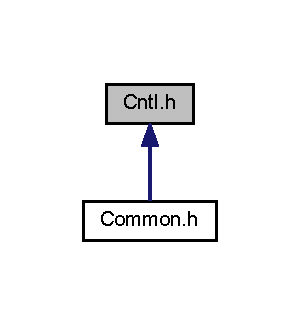
\includegraphics[width=350pt]{a00042}
\end{center}
\end{figure}


\subsection{Detailed Description}
Common include file for the project. All other header files used should be included within this file and this file should then be used to include them in the required source files. 
\hypertarget{a00010}{\section{xfmr\-Stage\-Settings Struct Reference}
\label{a00010}\index{xfmr\-Stage\-Settings@{xfmr\-Stage\-Settings}}
}


{\ttfamily \#include $<$Macro\-Nets.\-h$>$}

\subsection*{Data Fields}
\begin{DoxyCompactItemize}
\item 
int32 \hyperlink{a00010_a99d85a680a0b0b7f1858d77a3ac216b3}{ocp\-Level}
\item 
int32 \hyperlink{a00010_a40270e88484faa165e3e73f45c08326a}{mid\-Ovp\-Level}
\item 
int32 \hyperlink{a00010_a311d7915ed53ed668964b7664df881c0}{hv\-Ovp\-Level}
\item 
int32 \hyperlink{a00010_a582f0218997b0b37f365b75ae274e67c}{otp\-Level}
\item 
int16 \hyperlink{a00010_a7f041e2df9592fb461a013cdb67af348}{i\-Max}
\item 
int16 \hyperlink{a00010_a251fa7af71c610bf2b193afde33e1338}{mid\-V\-Max}
\item 
int16 \hyperlink{a00010_a55b65a695862a846307f5131b1220cbe}{hv\-V\-Max}
\item 
int16 \hyperlink{a00010_a3b4f123000ae32ca041c6286e5c92fd4}{i\-Scale}
\item 
int16 \hyperlink{a00010_a44cb584d774e345422c57cc155b65d0c}{mid\-V\-Scale}
\item 
int16 \hyperlink{a00010_a3a22ae7b7c6bf805037d571fce3652b8}{hv\-V\-Scale}
\item 
Uint16 \hyperlink{a00010_aef5e40360d79d34e95c2b412d4e4063b}{enable}
\end{DoxyCompactItemize}


\subsection{Detailed Description}
A structure that contains the settings that pertain to the transformer stage. 

\subsection{Field Documentation}
\hypertarget{a00010_aef5e40360d79d34e95c2b412d4e4063b}{\index{xfmr\-Stage\-Settings@{xfmr\-Stage\-Settings}!enable@{enable}}
\index{enable@{enable}!xfmrStageSettings@{xfmr\-Stage\-Settings}}
\subsubsection[{enable}]{\setlength{\rightskip}{0pt plus 5cm}Uint16 xfmr\-Stage\-Settings\-::enable}}\label{a00010_aef5e40360d79d34e95c2b412d4e4063b}
Channel enable status \{F\-A\-L\-S\-E, T\-R\-U\-E\}. \hypertarget{a00010_a311d7915ed53ed668964b7664df881c0}{\index{xfmr\-Stage\-Settings@{xfmr\-Stage\-Settings}!hv\-Ovp\-Level@{hv\-Ovp\-Level}}
\index{hv\-Ovp\-Level@{hv\-Ovp\-Level}!xfmrStageSettings@{xfmr\-Stage\-Settings}}
\subsubsection[{hv\-Ovp\-Level}]{\setlength{\rightskip}{0pt plus 5cm}int32 xfmr\-Stage\-Settings\-::hv\-Ovp\-Level}}\label{a00010_a311d7915ed53ed668964b7664df881c0}
Normalised D\-C H\-V O\-V\-P limit (I\-Q24). \hypertarget{a00010_a55b65a695862a846307f5131b1220cbe}{\index{xfmr\-Stage\-Settings@{xfmr\-Stage\-Settings}!hv\-V\-Max@{hv\-V\-Max}}
\index{hv\-V\-Max@{hv\-V\-Max}!xfmrStageSettings@{xfmr\-Stage\-Settings}}
\subsubsection[{hv\-V\-Max}]{\setlength{\rightskip}{0pt plus 5cm}int16 xfmr\-Stage\-Settings\-::hv\-V\-Max}}\label{a00010_a55b65a695862a846307f5131b1220cbe}
Maximum D\-C H\-V voltage setting limit (S\-Q10). \hypertarget{a00010_a3a22ae7b7c6bf805037d571fce3652b8}{\index{xfmr\-Stage\-Settings@{xfmr\-Stage\-Settings}!hv\-V\-Scale@{hv\-V\-Scale}}
\index{hv\-V\-Scale@{hv\-V\-Scale}!xfmrStageSettings@{xfmr\-Stage\-Settings}}
\subsubsection[{hv\-V\-Scale}]{\setlength{\rightskip}{0pt plus 5cm}int16 xfmr\-Stage\-Settings\-::hv\-V\-Scale}}\label{a00010_a3a22ae7b7c6bf805037d571fce3652b8}
D\-C H\-V voltage scaling setting in volts-\/per-\/volts for scaling between a voltage level measured by an A\-D\-C to a real voltage value (S\-Q14). \hypertarget{a00010_a7f041e2df9592fb461a013cdb67af348}{\index{xfmr\-Stage\-Settings@{xfmr\-Stage\-Settings}!i\-Max@{i\-Max}}
\index{i\-Max@{i\-Max}!xfmrStageSettings@{xfmr\-Stage\-Settings}}
\subsubsection[{i\-Max}]{\setlength{\rightskip}{0pt plus 5cm}int16 xfmr\-Stage\-Settings\-::i\-Max}}\label{a00010_a7f041e2df9592fb461a013cdb67af348}
Maximum D\-C current setting limit (S\-Q10). \hypertarget{a00010_a3b4f123000ae32ca041c6286e5c92fd4}{\index{xfmr\-Stage\-Settings@{xfmr\-Stage\-Settings}!i\-Scale@{i\-Scale}}
\index{i\-Scale@{i\-Scale}!xfmrStageSettings@{xfmr\-Stage\-Settings}}
\subsubsection[{i\-Scale}]{\setlength{\rightskip}{0pt plus 5cm}int16 xfmr\-Stage\-Settings\-::i\-Scale}}\label{a00010_a3b4f123000ae32ca041c6286e5c92fd4}
Current scaling setting in volts-\/per-\/amp for scaling between a voltage level measured by an A\-D\-C to a real current value (S\-Q14). \hypertarget{a00010_a40270e88484faa165e3e73f45c08326a}{\index{xfmr\-Stage\-Settings@{xfmr\-Stage\-Settings}!mid\-Ovp\-Level@{mid\-Ovp\-Level}}
\index{mid\-Ovp\-Level@{mid\-Ovp\-Level}!xfmrStageSettings@{xfmr\-Stage\-Settings}}
\subsubsection[{mid\-Ovp\-Level}]{\setlength{\rightskip}{0pt plus 5cm}int32 xfmr\-Stage\-Settings\-::mid\-Ovp\-Level}}\label{a00010_a40270e88484faa165e3e73f45c08326a}
Normalised D\-C mid O\-V\-P limit (I\-Q24). \hypertarget{a00010_a251fa7af71c610bf2b193afde33e1338}{\index{xfmr\-Stage\-Settings@{xfmr\-Stage\-Settings}!mid\-V\-Max@{mid\-V\-Max}}
\index{mid\-V\-Max@{mid\-V\-Max}!xfmrStageSettings@{xfmr\-Stage\-Settings}}
\subsubsection[{mid\-V\-Max}]{\setlength{\rightskip}{0pt plus 5cm}int16 xfmr\-Stage\-Settings\-::mid\-V\-Max}}\label{a00010_a251fa7af71c610bf2b193afde33e1338}
Maximum D\-C mid voltage setting limit (S\-Q10). \hypertarget{a00010_a44cb584d774e345422c57cc155b65d0c}{\index{xfmr\-Stage\-Settings@{xfmr\-Stage\-Settings}!mid\-V\-Scale@{mid\-V\-Scale}}
\index{mid\-V\-Scale@{mid\-V\-Scale}!xfmrStageSettings@{xfmr\-Stage\-Settings}}
\subsubsection[{mid\-V\-Scale}]{\setlength{\rightskip}{0pt plus 5cm}int16 xfmr\-Stage\-Settings\-::mid\-V\-Scale}}\label{a00010_a44cb584d774e345422c57cc155b65d0c}
D\-C mid voltage scaling setting in volts-\/per-\/volts for scaling between a voltage level measured by an A\-D\-C to a real voltage value (S\-Q14). \hypertarget{a00010_a99d85a680a0b0b7f1858d77a3ac216b3}{\index{xfmr\-Stage\-Settings@{xfmr\-Stage\-Settings}!ocp\-Level@{ocp\-Level}}
\index{ocp\-Level@{ocp\-Level}!xfmrStageSettings@{xfmr\-Stage\-Settings}}
\subsubsection[{ocp\-Level}]{\setlength{\rightskip}{0pt plus 5cm}int32 xfmr\-Stage\-Settings\-::ocp\-Level}}\label{a00010_a99d85a680a0b0b7f1858d77a3ac216b3}
Normalised O\-C\-P limit (I\-Q24). \hypertarget{a00010_a582f0218997b0b37f365b75ae274e67c}{\index{xfmr\-Stage\-Settings@{xfmr\-Stage\-Settings}!otp\-Level@{otp\-Level}}
\index{otp\-Level@{otp\-Level}!xfmrStageSettings@{xfmr\-Stage\-Settings}}
\subsubsection[{otp\-Level}]{\setlength{\rightskip}{0pt plus 5cm}int32 xfmr\-Stage\-Settings\-::otp\-Level}}\label{a00010_a582f0218997b0b37f365b75ae274e67c}
O\-T\-P limit in $ ^\circ$ C (S\-Q7). 

The documentation for this struct was generated from the following file\-:\begin{DoxyCompactItemize}
\item 
\hyperlink{a00027}{Macro\-Nets.\-h}\end{DoxyCompactItemize}

\chapter{File Documentation}
\hypertarget{a00012}{\section{Fan\-En.\-h File Reference}
\label{a00012}\index{Fan\-En.\-h@{Fan\-En.\-h}}
}


Functions for enabling and disabling the external fans via I2\-C.  


This graph shows which files directly or indirectly include this file\-:
\nopagebreak
\begin{figure}[H]
\begin{center}
\leavevmode
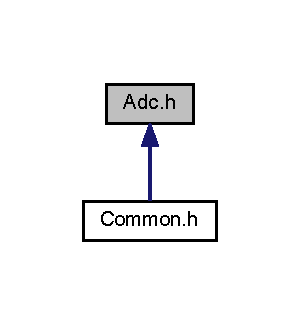
\includegraphics[width=144pt]{a00043}
\end{center}
\end{figure}
\subsection*{Macros}
\begin{DoxyCompactItemize}
\item 
\#define \hyperlink{a00012_ad615a329bea187ce779cf9930ba8a6fa}{I\-O\-E\-\_\-\-I2\-C\-\_\-\-A\-D\-D\-R}~0x20
\item 
\#define \hyperlink{a00012_a36c134b088cc2e64e0a5e14e8f90fe38}{I\-O\-E\-\_\-\-I\-O\-D\-I\-R\-\_\-\-A\-D\-D\-R}~0x00
\item 
\#define \hyperlink{a00012_a04633cd2ea7fd0b332e1edf066f674c4}{I\-O\-E\-\_\-\-I\-P\-O\-L\-\_\-\-A\-D\-D\-R}~0x01
\item 
\#define \hyperlink{a00012_aa68be5a6ed28fb146600b4fd2d11fafd}{I\-O\-E\-\_\-\-G\-P\-I\-N\-T\-E\-N\-\_\-\-A\-D\-D\-R}~0x02
\item 
\#define \hyperlink{a00012_a687e15212e8d4b49c12159dce73eeeab}{I\-O\-E\-\_\-\-D\-E\-F\-V\-A\-L\-\_\-\-A\-D\-D\-R}~0x03
\item 
\#define \hyperlink{a00012_a90945d9544eebc892154f1e0443b1407}{I\-O\-E\-\_\-\-I\-N\-T\-C\-O\-N\-\_\-\-A\-D\-D\-R}~0x04
\item 
\#define \hyperlink{a00012_af44ed2bf93808aeb932ce9944a942b75}{I\-O\-E\-\_\-\-I\-O\-C\-O\-N\-\_\-\-A\-D\-D\-R}~0x05
\item 
\#define \hyperlink{a00012_a91e588d697383f94de2bf7f11d9ecb4b}{I\-O\-E\-\_\-\-G\-P\-P\-U\-\_\-\-A\-D\-D\-R}~0x06
\item 
\#define \hyperlink{a00012_a32cac2ad5af58a2562540ec8fc205dd1}{I\-O\-E\-\_\-\-I\-N\-T\-F\-\_\-\-A\-D\-D\-R}~0x07
\item 
\#define \hyperlink{a00012_ac0afd8503a8584599cc81f3d9b0a04dc}{I\-O\-E\-\_\-\-I\-N\-T\-C\-A\-P\-\_\-\-A\-D\-D\-R}~0x08
\item 
\#define \hyperlink{a00012_af2d85152c5775a221f107d6de547bca1}{I\-O\-E\-\_\-\-G\-P\-I\-O\-\_\-\-A\-D\-D\-R}~0x09
\item 
\#define \hyperlink{a00012_ab26864d7372ac11db9c1996842a3cf56}{I\-O\-E\-\_\-\-O\-L\-A\-T\-\_\-\-A\-D\-D\-R}~0x0\-A
\item 
\#define \hyperlink{a00012_a24c7360527d594acd521520c99b3de1b}{F\-A\-N\-\_\-\-N\-U\-M\-\_\-\-C\-H\-N\-L}~0x04
\item 
\#define \hyperlink{a00012_a8ccf236abd5b2b9bbf73007968077e3d}{F\-A\-N\-\_\-\-C\-H\-N\-L\-\_\-\-O\-F\-S\-T}~0x04
\end{DoxyCompactItemize}
\subsection*{Functions}
\begin{DoxyCompactItemize}
\item 
Uint16 \hyperlink{a00012_a3506b5e25346351ce292e2ad256607cc}{fc\-Init} (void)
\item 
Uint16 \hyperlink{a00012_a68c8852e37fd686fda74e593ecd71915}{fc\-Enable} (Uint16 chnl)
\item 
Uint16 \hyperlink{a00012_ac781d303e240f077d206088806a75ccd}{fc\-Disable} (Uint16 chnl)
\end{DoxyCompactItemize}


\subsection{Detailed Description}
Functions for enabling and disabling the external fans via I2\-C. The fans are controlled via an external I/\-O expander (M\-C\-P23008) that is connected to the I2\-C bus at address 0100x-\/x-\/x where 'x-\/x-\/x' is dependent upon the configuration of resistors R60 -\/ 61 \& R70 -\/ R74.

After \hyperlink{a00012_a3506b5e25346351ce292e2ad256607cc}{fc\-Init()} all fans default to disabled.

\begin{DoxyWarning}{Warning}
Before any fan control functions can be used the I2\-C peripheral M\-U\-S\-T be initialised and E\-I\-T\-H\-E\-R \hyperlink{a00012_a3506b5e25346351ce292e2ad256607cc}{fc\-Init()} or \hyperlink{a00006_aa6cb02a7aacce8671212b21ed6e39863}{bc\-Init()} must be run -\/ \hyperlink{a00012_a3506b5e25346351ce292e2ad256607cc}{fc\-Init()} will require the interrupts to be enabled globally.
\end{DoxyWarning}
\begin{DoxySeeAlso}{See Also}
\hyperlink{a00014_a1e0a81a1ad1fd7710ca189236e3e5476}{i2c\-Init()} 

\hyperlink{a00006_aa6cb02a7aacce8671212b21ed6e39863}{bc\-Init()} 
\end{DoxySeeAlso}


\subsection{Macro Definition Documentation}
\hypertarget{a00012_a8ccf236abd5b2b9bbf73007968077e3d}{\index{Fan\-En.\-h@{Fan\-En.\-h}!F\-A\-N\-\_\-\-C\-H\-N\-L\-\_\-\-O\-F\-S\-T@{F\-A\-N\-\_\-\-C\-H\-N\-L\-\_\-\-O\-F\-S\-T}}
\index{F\-A\-N\-\_\-\-C\-H\-N\-L\-\_\-\-O\-F\-S\-T@{F\-A\-N\-\_\-\-C\-H\-N\-L\-\_\-\-O\-F\-S\-T}!FanEn.h@{Fan\-En.\-h}}
\subsubsection[{F\-A\-N\-\_\-\-C\-H\-N\-L\-\_\-\-O\-F\-S\-T}]{\setlength{\rightskip}{0pt plus 5cm}\#define F\-A\-N\-\_\-\-C\-H\-N\-L\-\_\-\-O\-F\-S\-T~0x04}}\label{a00012_a8ccf236abd5b2b9bbf73007968077e3d}
Fan channel numbering offset \hypertarget{a00012_a24c7360527d594acd521520c99b3de1b}{\index{Fan\-En.\-h@{Fan\-En.\-h}!F\-A\-N\-\_\-\-N\-U\-M\-\_\-\-C\-H\-N\-L@{F\-A\-N\-\_\-\-N\-U\-M\-\_\-\-C\-H\-N\-L}}
\index{F\-A\-N\-\_\-\-N\-U\-M\-\_\-\-C\-H\-N\-L@{F\-A\-N\-\_\-\-N\-U\-M\-\_\-\-C\-H\-N\-L}!FanEn.h@{Fan\-En.\-h}}
\subsubsection[{F\-A\-N\-\_\-\-N\-U\-M\-\_\-\-C\-H\-N\-L}]{\setlength{\rightskip}{0pt plus 5cm}\#define F\-A\-N\-\_\-\-N\-U\-M\-\_\-\-C\-H\-N\-L~0x04}}\label{a00012_a24c7360527d594acd521520c99b3de1b}
Number of fan channels \hypertarget{a00012_a687e15212e8d4b49c12159dce73eeeab}{\index{Fan\-En.\-h@{Fan\-En.\-h}!I\-O\-E\-\_\-\-D\-E\-F\-V\-A\-L\-\_\-\-A\-D\-D\-R@{I\-O\-E\-\_\-\-D\-E\-F\-V\-A\-L\-\_\-\-A\-D\-D\-R}}
\index{I\-O\-E\-\_\-\-D\-E\-F\-V\-A\-L\-\_\-\-A\-D\-D\-R@{I\-O\-E\-\_\-\-D\-E\-F\-V\-A\-L\-\_\-\-A\-D\-D\-R}!FanEn.h@{Fan\-En.\-h}}
\subsubsection[{I\-O\-E\-\_\-\-D\-E\-F\-V\-A\-L\-\_\-\-A\-D\-D\-R}]{\setlength{\rightskip}{0pt plus 5cm}\#define I\-O\-E\-\_\-\-D\-E\-F\-V\-A\-L\-\_\-\-A\-D\-D\-R~0x03}}\label{a00012_a687e15212e8d4b49c12159dce73eeeab}
M\-C\-P23008 I/\-O expander default value register address \hypertarget{a00012_aa68be5a6ed28fb146600b4fd2d11fafd}{\index{Fan\-En.\-h@{Fan\-En.\-h}!I\-O\-E\-\_\-\-G\-P\-I\-N\-T\-E\-N\-\_\-\-A\-D\-D\-R@{I\-O\-E\-\_\-\-G\-P\-I\-N\-T\-E\-N\-\_\-\-A\-D\-D\-R}}
\index{I\-O\-E\-\_\-\-G\-P\-I\-N\-T\-E\-N\-\_\-\-A\-D\-D\-R@{I\-O\-E\-\_\-\-G\-P\-I\-N\-T\-E\-N\-\_\-\-A\-D\-D\-R}!FanEn.h@{Fan\-En.\-h}}
\subsubsection[{I\-O\-E\-\_\-\-G\-P\-I\-N\-T\-E\-N\-\_\-\-A\-D\-D\-R}]{\setlength{\rightskip}{0pt plus 5cm}\#define I\-O\-E\-\_\-\-G\-P\-I\-N\-T\-E\-N\-\_\-\-A\-D\-D\-R~0x02}}\label{a00012_aa68be5a6ed28fb146600b4fd2d11fafd}
M\-C\-P23008 I/\-O expander interrupt on change enable register address \hypertarget{a00012_af2d85152c5775a221f107d6de547bca1}{\index{Fan\-En.\-h@{Fan\-En.\-h}!I\-O\-E\-\_\-\-G\-P\-I\-O\-\_\-\-A\-D\-D\-R@{I\-O\-E\-\_\-\-G\-P\-I\-O\-\_\-\-A\-D\-D\-R}}
\index{I\-O\-E\-\_\-\-G\-P\-I\-O\-\_\-\-A\-D\-D\-R@{I\-O\-E\-\_\-\-G\-P\-I\-O\-\_\-\-A\-D\-D\-R}!FanEn.h@{Fan\-En.\-h}}
\subsubsection[{I\-O\-E\-\_\-\-G\-P\-I\-O\-\_\-\-A\-D\-D\-R}]{\setlength{\rightskip}{0pt plus 5cm}\#define I\-O\-E\-\_\-\-G\-P\-I\-O\-\_\-\-A\-D\-D\-R~0x09}}\label{a00012_af2d85152c5775a221f107d6de547bca1}
M\-C\-P23008 I/\-O expander G\-P\-I\-O port register address \hypertarget{a00012_a91e588d697383f94de2bf7f11d9ecb4b}{\index{Fan\-En.\-h@{Fan\-En.\-h}!I\-O\-E\-\_\-\-G\-P\-P\-U\-\_\-\-A\-D\-D\-R@{I\-O\-E\-\_\-\-G\-P\-P\-U\-\_\-\-A\-D\-D\-R}}
\index{I\-O\-E\-\_\-\-G\-P\-P\-U\-\_\-\-A\-D\-D\-R@{I\-O\-E\-\_\-\-G\-P\-P\-U\-\_\-\-A\-D\-D\-R}!FanEn.h@{Fan\-En.\-h}}
\subsubsection[{I\-O\-E\-\_\-\-G\-P\-P\-U\-\_\-\-A\-D\-D\-R}]{\setlength{\rightskip}{0pt plus 5cm}\#define I\-O\-E\-\_\-\-G\-P\-P\-U\-\_\-\-A\-D\-D\-R~0x06}}\label{a00012_a91e588d697383f94de2bf7f11d9ecb4b}
M\-C\-P23008 I/\-O expander pull-\/up resistor configuration register address \hypertarget{a00012_ad615a329bea187ce779cf9930ba8a6fa}{\index{Fan\-En.\-h@{Fan\-En.\-h}!I\-O\-E\-\_\-\-I2\-C\-\_\-\-A\-D\-D\-R@{I\-O\-E\-\_\-\-I2\-C\-\_\-\-A\-D\-D\-R}}
\index{I\-O\-E\-\_\-\-I2\-C\-\_\-\-A\-D\-D\-R@{I\-O\-E\-\_\-\-I2\-C\-\_\-\-A\-D\-D\-R}!FanEn.h@{Fan\-En.\-h}}
\subsubsection[{I\-O\-E\-\_\-\-I2\-C\-\_\-\-A\-D\-D\-R}]{\setlength{\rightskip}{0pt plus 5cm}\#define I\-O\-E\-\_\-\-I2\-C\-\_\-\-A\-D\-D\-R~0x20}}\label{a00012_ad615a329bea187ce779cf9930ba8a6fa}
M\-C\-P23008 I/\-O expander I2\-C address (slave, 32d, 8-\/bit I/\-O expander) \hypertarget{a00012_ac0afd8503a8584599cc81f3d9b0a04dc}{\index{Fan\-En.\-h@{Fan\-En.\-h}!I\-O\-E\-\_\-\-I\-N\-T\-C\-A\-P\-\_\-\-A\-D\-D\-R@{I\-O\-E\-\_\-\-I\-N\-T\-C\-A\-P\-\_\-\-A\-D\-D\-R}}
\index{I\-O\-E\-\_\-\-I\-N\-T\-C\-A\-P\-\_\-\-A\-D\-D\-R@{I\-O\-E\-\_\-\-I\-N\-T\-C\-A\-P\-\_\-\-A\-D\-D\-R}!FanEn.h@{Fan\-En.\-h}}
\subsubsection[{I\-O\-E\-\_\-\-I\-N\-T\-C\-A\-P\-\_\-\-A\-D\-D\-R}]{\setlength{\rightskip}{0pt plus 5cm}\#define I\-O\-E\-\_\-\-I\-N\-T\-C\-A\-P\-\_\-\-A\-D\-D\-R~0x08}}\label{a00012_ac0afd8503a8584599cc81f3d9b0a04dc}
M\-C\-P23008 I/\-O expander interrupt capture register address \hypertarget{a00012_a90945d9544eebc892154f1e0443b1407}{\index{Fan\-En.\-h@{Fan\-En.\-h}!I\-O\-E\-\_\-\-I\-N\-T\-C\-O\-N\-\_\-\-A\-D\-D\-R@{I\-O\-E\-\_\-\-I\-N\-T\-C\-O\-N\-\_\-\-A\-D\-D\-R}}
\index{I\-O\-E\-\_\-\-I\-N\-T\-C\-O\-N\-\_\-\-A\-D\-D\-R@{I\-O\-E\-\_\-\-I\-N\-T\-C\-O\-N\-\_\-\-A\-D\-D\-R}!FanEn.h@{Fan\-En.\-h}}
\subsubsection[{I\-O\-E\-\_\-\-I\-N\-T\-C\-O\-N\-\_\-\-A\-D\-D\-R}]{\setlength{\rightskip}{0pt plus 5cm}\#define I\-O\-E\-\_\-\-I\-N\-T\-C\-O\-N\-\_\-\-A\-D\-D\-R~0x04}}\label{a00012_a90945d9544eebc892154f1e0443b1407}
M\-C\-P23008 I/\-O expander interrupt on change control register address \hypertarget{a00012_a32cac2ad5af58a2562540ec8fc205dd1}{\index{Fan\-En.\-h@{Fan\-En.\-h}!I\-O\-E\-\_\-\-I\-N\-T\-F\-\_\-\-A\-D\-D\-R@{I\-O\-E\-\_\-\-I\-N\-T\-F\-\_\-\-A\-D\-D\-R}}
\index{I\-O\-E\-\_\-\-I\-N\-T\-F\-\_\-\-A\-D\-D\-R@{I\-O\-E\-\_\-\-I\-N\-T\-F\-\_\-\-A\-D\-D\-R}!FanEn.h@{Fan\-En.\-h}}
\subsubsection[{I\-O\-E\-\_\-\-I\-N\-T\-F\-\_\-\-A\-D\-D\-R}]{\setlength{\rightskip}{0pt plus 5cm}\#define I\-O\-E\-\_\-\-I\-N\-T\-F\-\_\-\-A\-D\-D\-R~0x07}}\label{a00012_a32cac2ad5af58a2562540ec8fc205dd1}
M\-C\-P23008 I/\-O expander interrupt flag register address \hypertarget{a00012_af44ed2bf93808aeb932ce9944a942b75}{\index{Fan\-En.\-h@{Fan\-En.\-h}!I\-O\-E\-\_\-\-I\-O\-C\-O\-N\-\_\-\-A\-D\-D\-R@{I\-O\-E\-\_\-\-I\-O\-C\-O\-N\-\_\-\-A\-D\-D\-R}}
\index{I\-O\-E\-\_\-\-I\-O\-C\-O\-N\-\_\-\-A\-D\-D\-R@{I\-O\-E\-\_\-\-I\-O\-C\-O\-N\-\_\-\-A\-D\-D\-R}!FanEn.h@{Fan\-En.\-h}}
\subsubsection[{I\-O\-E\-\_\-\-I\-O\-C\-O\-N\-\_\-\-A\-D\-D\-R}]{\setlength{\rightskip}{0pt plus 5cm}\#define I\-O\-E\-\_\-\-I\-O\-C\-O\-N\-\_\-\-A\-D\-D\-R~0x05}}\label{a00012_af44ed2bf93808aeb932ce9944a942b75}
M\-C\-P23008 I/\-O expander configuration register address \hypertarget{a00012_a36c134b088cc2e64e0a5e14e8f90fe38}{\index{Fan\-En.\-h@{Fan\-En.\-h}!I\-O\-E\-\_\-\-I\-O\-D\-I\-R\-\_\-\-A\-D\-D\-R@{I\-O\-E\-\_\-\-I\-O\-D\-I\-R\-\_\-\-A\-D\-D\-R}}
\index{I\-O\-E\-\_\-\-I\-O\-D\-I\-R\-\_\-\-A\-D\-D\-R@{I\-O\-E\-\_\-\-I\-O\-D\-I\-R\-\_\-\-A\-D\-D\-R}!FanEn.h@{Fan\-En.\-h}}
\subsubsection[{I\-O\-E\-\_\-\-I\-O\-D\-I\-R\-\_\-\-A\-D\-D\-R}]{\setlength{\rightskip}{0pt plus 5cm}\#define I\-O\-E\-\_\-\-I\-O\-D\-I\-R\-\_\-\-A\-D\-D\-R~0x00}}\label{a00012_a36c134b088cc2e64e0a5e14e8f90fe38}
M\-C\-P23008 I/\-O expander I/\-O direction register address \hypertarget{a00012_a04633cd2ea7fd0b332e1edf066f674c4}{\index{Fan\-En.\-h@{Fan\-En.\-h}!I\-O\-E\-\_\-\-I\-P\-O\-L\-\_\-\-A\-D\-D\-R@{I\-O\-E\-\_\-\-I\-P\-O\-L\-\_\-\-A\-D\-D\-R}}
\index{I\-O\-E\-\_\-\-I\-P\-O\-L\-\_\-\-A\-D\-D\-R@{I\-O\-E\-\_\-\-I\-P\-O\-L\-\_\-\-A\-D\-D\-R}!FanEn.h@{Fan\-En.\-h}}
\subsubsection[{I\-O\-E\-\_\-\-I\-P\-O\-L\-\_\-\-A\-D\-D\-R}]{\setlength{\rightskip}{0pt plus 5cm}\#define I\-O\-E\-\_\-\-I\-P\-O\-L\-\_\-\-A\-D\-D\-R~0x01}}\label{a00012_a04633cd2ea7fd0b332e1edf066f674c4}
M\-C\-P23008 I/\-O expander input polarity register address \hypertarget{a00012_ab26864d7372ac11db9c1996842a3cf56}{\index{Fan\-En.\-h@{Fan\-En.\-h}!I\-O\-E\-\_\-\-O\-L\-A\-T\-\_\-\-A\-D\-D\-R@{I\-O\-E\-\_\-\-O\-L\-A\-T\-\_\-\-A\-D\-D\-R}}
\index{I\-O\-E\-\_\-\-O\-L\-A\-T\-\_\-\-A\-D\-D\-R@{I\-O\-E\-\_\-\-O\-L\-A\-T\-\_\-\-A\-D\-D\-R}!FanEn.h@{Fan\-En.\-h}}
\subsubsection[{I\-O\-E\-\_\-\-O\-L\-A\-T\-\_\-\-A\-D\-D\-R}]{\setlength{\rightskip}{0pt plus 5cm}\#define I\-O\-E\-\_\-\-O\-L\-A\-T\-\_\-\-A\-D\-D\-R~0x0\-A}}\label{a00012_ab26864d7372ac11db9c1996842a3cf56}
M\-C\-P23008 I/\-O expander output latch register address 

\subsection{Function Documentation}
\hypertarget{a00012_ac781d303e240f077d206088806a75ccd}{\index{Fan\-En.\-h@{Fan\-En.\-h}!fc\-Disable@{fc\-Disable}}
\index{fc\-Disable@{fc\-Disable}!FanEn.h@{Fan\-En.\-h}}
\subsubsection[{fc\-Disable}]{\setlength{\rightskip}{0pt plus 5cm}Uint16 fc\-Disable (
\begin{DoxyParamCaption}
\item[{Uint16}]{chnl}
\end{DoxyParamCaption}
)}}\label{a00012_ac781d303e240f077d206088806a75ccd}
Disables the specified channel's fan The I2\-C peripheral and the fan enable controller interface M\-U\-S\-T be initialised before this function is used. \begin{DoxySeeAlso}{See Also}
\hyperlink{a00014_a1e0a81a1ad1fd7710ca189236e3e5476}{i2c\-Init()} 

\hyperlink{a00012_a3506b5e25346351ce292e2ad256607cc}{fc\-Init()} 
\end{DoxySeeAlso}

\begin{DoxyParams}[1]{Parameters}
\mbox{\tt in}  & {\em chnl} & Specifies the channel fan that is to be disabled \\
\hline
\end{DoxyParams}
\begin{DoxyReturn}{Returns}
Error status 
\end{DoxyReturn}
\hypertarget{a00012_a68c8852e37fd686fda74e593ecd71915}{\index{Fan\-En.\-h@{Fan\-En.\-h}!fc\-Enable@{fc\-Enable}}
\index{fc\-Enable@{fc\-Enable}!FanEn.h@{Fan\-En.\-h}}
\subsubsection[{fc\-Enable}]{\setlength{\rightskip}{0pt plus 5cm}Uint16 fc\-Enable (
\begin{DoxyParamCaption}
\item[{Uint16}]{chnl}
\end{DoxyParamCaption}
)}}\label{a00012_a68c8852e37fd686fda74e593ecd71915}
Enables the specified channel's fan The I2\-C peripheral and the fan enable controller interface M\-U\-S\-T be initialised before this function is used. \begin{DoxySeeAlso}{See Also}
\hyperlink{a00014_a1e0a81a1ad1fd7710ca189236e3e5476}{i2c\-Init()} 

\hyperlink{a00012_a3506b5e25346351ce292e2ad256607cc}{fc\-Init()} 
\end{DoxySeeAlso}

\begin{DoxyParams}[1]{Parameters}
\mbox{\tt in}  & {\em chnl} & Specifies the channel fan that is to be enabled \\
\hline
\end{DoxyParams}
\begin{DoxyReturn}{Returns}
Error status 
\end{DoxyReturn}
\hypertarget{a00012_a3506b5e25346351ce292e2ad256607cc}{\index{Fan\-En.\-h@{Fan\-En.\-h}!fc\-Init@{fc\-Init}}
\index{fc\-Init@{fc\-Init}!FanEn.h@{Fan\-En.\-h}}
\subsubsection[{fc\-Init}]{\setlength{\rightskip}{0pt plus 5cm}Uint16 fc\-Init (
\begin{DoxyParamCaption}
\item[{void}]{}
\end{DoxyParamCaption}
)}}\label{a00012_a3506b5e25346351ce292e2ad256607cc}
Initialises the fan enable control interface. The I2\-C peripheral must be initialised before this function is used. \begin{DoxySeeAlso}{See Also}
\hyperlink{a00014_a1e0a81a1ad1fd7710ca189236e3e5476}{i2c\-Init()} 
\end{DoxySeeAlso}
\begin{DoxyReturn}{Returns}
Error status 
\end{DoxyReturn}

\hypertarget{a00014}{\section{Cntl.\-h File Reference}
\label{a00014}\index{Cntl.\-h@{Cntl.\-h}}
}


D\-P\-Lib C\-N\-T\-L Macro related helper functions.  


This graph shows which files directly or indirectly include this file\-:\nopagebreak
\begin{figure}[H]
\begin{center}
\leavevmode
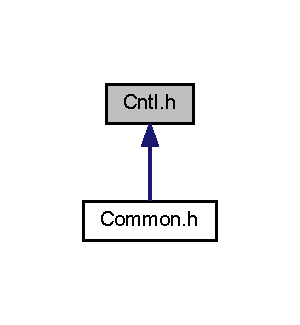
\includegraphics[width=144pt]{a00061}
\end{center}
\end{figure}
\subsection*{Typedefs}
\begin{DoxyCompactItemize}
\item 
typedef enum \hyperlink{a00014_a4b8f446b389413b175ff4d4dbcd18da1}{coef\-Num} \hyperlink{a00014_ac340fbbc5919954c173757935549588f}{cf\-Type}
\end{DoxyCompactItemize}
\subsection*{Enumerations}
\begin{DoxyCompactItemize}
\item 
enum \hyperlink{a00014_a4b8f446b389413b175ff4d4dbcd18da1}{coef\-Num} \{ , \\*
\hyperlink{a00014_a4b8f446b389413b175ff4d4dbcd18da1ad15b967851188a21b2d4fd326304bf83}{c\-Min} = first\-Coef, 
\hyperlink{a00014_a4b8f446b389413b175ff4d4dbcd18da1a3576a9eb4b8f9d1ca3d31a0f9b889299}{c\-Max}, 
\hyperlink{a00014_a4b8f446b389413b175ff4d4dbcd18da1a3dec162fc3f68f49f43775eba612e110}{c\-B0}, 
\hyperlink{a00014_a4b8f446b389413b175ff4d4dbcd18da1a43986b141584b760c8c8c9fc29304de2}{c\-B1}, 
\\*
\hyperlink{a00014_a4b8f446b389413b175ff4d4dbcd18da1aac28a7344b33c5e968a79fc27078da99}{c\-A1}, 
\hyperlink{a00014_a4b8f446b389413b175ff4d4dbcd18da1a5229cb73bab727c5aeaae425a4fd2472}{c\-B2}, 
\hyperlink{a00014_a4b8f446b389413b175ff4d4dbcd18da1a80d8d6d72b42fa8603b71cba71e13ef2}{c\-A2}
 \}
\end{DoxyCompactItemize}
\subsection*{Functions}
\begin{DoxyCompactItemize}
\item 
void \hyperlink{a00014_a91a941a20fc5a9465397d4701e0beaf4}{init\-Coefs} (void)
\item 
Uint16 \hyperlink{a00014_ac551a1fee10631510b139d6d97bb166c}{set\-Load\-I\-Coef} (\hyperlink{a00027_a2820f1e18d921d2f1e97d53404b9fbae}{load\-Stage} load, \hyperlink{a00014_ac340fbbc5919954c173757935549588f}{cf\-Type} coef, float32 value)
\item 
Uint16 \hyperlink{a00014_a86bea9827291d6230b0f3366bbd8ce27}{get\-Load\-I\-Coef} (\hyperlink{a00027_a2820f1e18d921d2f1e97d53404b9fbae}{load\-Stage} load, \hyperlink{a00014_ac340fbbc5919954c173757935549588f}{cf\-Type} coef, float32 $\ast$value)
\item 
Uint16 \hyperlink{a00014_a8f635eee5f9c27a4f7d4349334b5ee78}{set\-Ac\-I\-Coef} (\hyperlink{a00014_ac340fbbc5919954c173757935549588f}{cf\-Type} coef, float32 val)
\item 
Uint16 \hyperlink{a00014_a766238d36085cd55f37f88fd8b2bb110}{get\-Ac\-I\-Coef} (\hyperlink{a00014_ac340fbbc5919954c173757935549588f}{cf\-Type} coef, float32 $\ast$value)
\item 
Uint16 \hyperlink{a00014_acaa99aafbcfaf6399a815e094c431474}{set\-Ac\-V\-Coef} (\hyperlink{a00014_ac340fbbc5919954c173757935549588f}{cf\-Type} coef, float32 value)
\item 
Uint16 \hyperlink{a00014_ad3161240a1aa23145fcba9506cb9001c}{get\-Ac\-V\-Coef} (\hyperlink{a00014_ac340fbbc5919954c173757935549588f}{cf\-Type} coef, float32 $\ast$value)
\end{DoxyCompactItemize}
\subsection*{Variables}
\begin{DoxyCompactItemize}
\item 
struct C\-N\-T\-L\-\_\-2\-P2\-Z\-\_\-\-Coef\-Struct \hyperlink{a00014_af15987bb0b6b0819b233fa6963671a35}{load\-I\-Coefs} \mbox{[}number\-Of\-Loads\mbox{]}
\item 
struct C\-N\-T\-L\-\_\-2\-P2\-Z\-\_\-\-Coef\-Struct \hyperlink{a00014_a05ea1ba581ea8bf1eb5c44f15534d31c}{ac\-I\-Coefs}
\item 
struct C\-N\-T\-L\-\_\-2\-P2\-Z\-\_\-\-Coef\-Struct \hyperlink{a00014_a07dbef418ea85cb169ebfc52e9571d68}{ac\-V\-Coefs}
\item 
volatile int32 $\ast$ \hyperlink{a00014_a047c759a71b80d8cfd5e6f52b1b021b9}{C\-N\-T\-L\-\_\-2\-P2\-Z\-\_\-\-Coef1}
\item 
volatile int32 $\ast$ \hyperlink{a00014_abdc599cbabc62898c49926678c3327e6}{C\-N\-T\-L\-\_\-2\-P2\-Z\-\_\-\-Coef2}
\item 
volatile int32 $\ast$ \hyperlink{a00014_a1e357d296e76299ea04d7a63e4c46d1b}{C\-N\-T\-L\-\_\-2\-P2\-Z\-\_\-\-Coef3}
\item 
volatile int32 $\ast$ \hyperlink{a00014_afe468cb1e995b267671e88b8d292aef6}{C\-N\-T\-L\-\_\-2\-P2\-Z\-\_\-\-Coef4}
\item 
volatile int32 $\ast$ \hyperlink{a00014_a9c0418a780375035750c3d4dc16f3ae4}{C\-N\-T\-L\-\_\-2\-P2\-Z\-\_\-\-Fdbk1}
\item 
volatile int32 $\ast$ \hyperlink{a00014_a6092ef1c1c54802bb5e11564f782390d}{C\-N\-T\-L\-\_\-2\-P2\-Z\-\_\-\-Fdbk2}
\item 
volatile int32 $\ast$ \hyperlink{a00014_a939782d23ddbf7f45e5e393a65bafcff}{C\-N\-T\-L\-\_\-2\-P2\-Z\-\_\-\-Fdbk3}
\item 
volatile int32 $\ast$ \hyperlink{a00014_a6937e965f3ae840ea6ee43cce410680f}{C\-N\-T\-L\-\_\-2\-P2\-Z\-\_\-\-Fdbk4}
\item 
volatile int32 $\ast$ \hyperlink{a00014_a84d7c096ca668d1edc5e4fa54abe5d98}{C\-N\-T\-L\-\_\-2\-P2\-Z\-\_\-\-Out1}
\item 
volatile int32 $\ast$ \hyperlink{a00014_ae6679b66ffeca93742f973a2c947855f}{C\-N\-T\-L\-\_\-2\-P2\-Z\-\_\-\-Out2}
\item 
volatile int32 $\ast$ \hyperlink{a00014_a11dcb9f6b6d03fe960ddf790e1ad5ed2}{C\-N\-T\-L\-\_\-2\-P2\-Z\-\_\-\-Out3}
\item 
volatile int32 $\ast$ \hyperlink{a00014_a253e4070b19470606e0566ff25fc911f}{C\-N\-T\-L\-\_\-2\-P2\-Z\-\_\-\-Out4}
\item 
volatile int32 $\ast$ \hyperlink{a00014_a98527ce76f5175fa2933d46f324d85fb}{C\-N\-T\-L\-\_\-2\-P2\-Z\-\_\-\-Ref1}
\item 
volatile int32 $\ast$ \hyperlink{a00014_a9bf1756a901a3a74d9f43a51f85cede4}{C\-N\-T\-L\-\_\-2\-P2\-Z\-\_\-\-Ref2}
\item 
volatile int32 $\ast$ \hyperlink{a00014_a859e9bbd5bc82f1b42863a93e4f992af}{C\-N\-T\-L\-\_\-2\-P2\-Z\-\_\-\-Ref3}
\item 
volatile int32 $\ast$ \hyperlink{a00014_af54c55f228deb8189c44282a94a870c1}{C\-N\-T\-L\-\_\-2\-P2\-Z\-\_\-\-Ref4}
\item 
volatile int32 $\ast$ \hyperlink{a00014_a5fe3f4dd6aac27512c9e0b6fc843b0b6}{C\-N\-T\-L\-\_\-2\-P2\-Z\-\_\-\-Coef5}
\item 
volatile int32 $\ast$ \hyperlink{a00014_af5cbb635f31bbebd041e8543deb40dee}{C\-N\-T\-L\-\_\-2\-P2\-Z\-\_\-\-Fdbk5}
\item 
volatile int32 $\ast$ \hyperlink{a00014_a3b336a91d25a7feb9f8927b32b800d0d}{C\-N\-T\-L\-\_\-2\-P2\-Z\-\_\-\-Out5}
\item 
volatile int32 $\ast$ \hyperlink{a00014_abd3b240e2d3f7d3f4f717066ee8efd3e}{C\-N\-T\-L\-\_\-2\-P2\-Z\-\_\-\-Ref5}
\item 
volatile int32 $\ast$ \hyperlink{a00014_ac7b2d6195e1c497429235d54ebbd9087}{C\-N\-T\-L\-\_\-2\-P2\-Z\-\_\-\-Coef6}
\item 
volatile int32 $\ast$ \hyperlink{a00014_a1ce5f290e8eb4fd89ae9787e7020e062}{C\-N\-T\-L\-\_\-2\-P2\-Z\-\_\-\-Fdbk6}
\item 
volatile int32 $\ast$ \hyperlink{a00014_a3fa3864d3225e966af68bdea65781464}{C\-N\-T\-L\-\_\-2\-P2\-Z\-\_\-\-Out6}
\item 
volatile int32 $\ast$ \hyperlink{a00014_a2e5a137088ca653c5642c3bb9cbaec9d}{C\-N\-T\-L\-\_\-2\-P2\-Z\-\_\-\-Ref6}
\end{DoxyCompactItemize}


\subsection{Detailed Description}
D\-P\-Lib C\-N\-T\-L Macro related helper functions. 

\subsection{Typedef Documentation}
\hypertarget{a00014_ac340fbbc5919954c173757935549588f}{\index{Cntl.\-h@{Cntl.\-h}!cf\-Type@{cf\-Type}}
\index{cf\-Type@{cf\-Type}!Cntl.h@{Cntl.\-h}}
\subsubsection[{cf\-Type}]{\setlength{\rightskip}{0pt plus 5cm}typedef enum {\bf coef\-Num} {\bf cf\-Type}}}\label{a00014_ac340fbbc5919954c173757935549588f}
A type that allows a reference to a C\-N\-T\-L coefficient. 

\subsection{Enumeration Type Documentation}
\hypertarget{a00014_a4b8f446b389413b175ff4d4dbcd18da1}{\index{Cntl.\-h@{Cntl.\-h}!coef\-Num@{coef\-Num}}
\index{coef\-Num@{coef\-Num}!Cntl.h@{Cntl.\-h}}
\subsubsection[{coef\-Num}]{\setlength{\rightskip}{0pt plus 5cm}enum {\bf coef\-Num}}}\label{a00014_a4b8f446b389413b175ff4d4dbcd18da1}
C\-N\-T\-L Coefficient references \begin{Desc}
\item[Enumerator]\par
\begin{description}
\index{c\-Min@{c\-Min}!Cntl.\-h@{Cntl.\-h}}\index{Cntl.\-h@{Cntl.\-h}!c\-Min@{c\-Min}}\item[{\em 
\hypertarget{a00014_a4b8f446b389413b175ff4d4dbcd18da1ad15b967851188a21b2d4fd326304bf83}{c\-Min}\label{a00014_a4b8f446b389413b175ff4d4dbcd18da1ad15b967851188a21b2d4fd326304bf83}
}]Saturation minimum reference. \index{c\-Max@{c\-Max}!Cntl.\-h@{Cntl.\-h}}\index{Cntl.\-h@{Cntl.\-h}!c\-Max@{c\-Max}}\item[{\em 
\hypertarget{a00014_a4b8f446b389413b175ff4d4dbcd18da1a3576a9eb4b8f9d1ca3d31a0f9b889299}{c\-Max}\label{a00014_a4b8f446b389413b175ff4d4dbcd18da1a3576a9eb4b8f9d1ca3d31a0f9b889299}
}]Saturation maximum reference. \index{c\-B0@{c\-B0}!Cntl.\-h@{Cntl.\-h}}\index{Cntl.\-h@{Cntl.\-h}!c\-B0@{c\-B0}}\item[{\em 
\hypertarget{a00014_a4b8f446b389413b175ff4d4dbcd18da1a3dec162fc3f68f49f43775eba612e110}{c\-B0}\label{a00014_a4b8f446b389413b175ff4d4dbcd18da1a3dec162fc3f68f49f43775eba612e110}
}]B0 coefficient reference. \index{c\-B1@{c\-B1}!Cntl.\-h@{Cntl.\-h}}\index{Cntl.\-h@{Cntl.\-h}!c\-B1@{c\-B1}}\item[{\em 
\hypertarget{a00014_a4b8f446b389413b175ff4d4dbcd18da1a43986b141584b760c8c8c9fc29304de2}{c\-B1}\label{a00014_a4b8f446b389413b175ff4d4dbcd18da1a43986b141584b760c8c8c9fc29304de2}
}]B1 coefficient reference. \index{c\-A1@{c\-A1}!Cntl.\-h@{Cntl.\-h}}\index{Cntl.\-h@{Cntl.\-h}!c\-A1@{c\-A1}}\item[{\em 
\hypertarget{a00014_a4b8f446b389413b175ff4d4dbcd18da1aac28a7344b33c5e968a79fc27078da99}{c\-A1}\label{a00014_a4b8f446b389413b175ff4d4dbcd18da1aac28a7344b33c5e968a79fc27078da99}
}]A1 coefficient reference. \index{c\-B2@{c\-B2}!Cntl.\-h@{Cntl.\-h}}\index{Cntl.\-h@{Cntl.\-h}!c\-B2@{c\-B2}}\item[{\em 
\hypertarget{a00014_a4b8f446b389413b175ff4d4dbcd18da1a5229cb73bab727c5aeaae425a4fd2472}{c\-B2}\label{a00014_a4b8f446b389413b175ff4d4dbcd18da1a5229cb73bab727c5aeaae425a4fd2472}
}]B2 coefficient reference. \index{c\-A2@{c\-A2}!Cntl.\-h@{Cntl.\-h}}\index{Cntl.\-h@{Cntl.\-h}!c\-A2@{c\-A2}}\item[{\em 
\hypertarget{a00014_a4b8f446b389413b175ff4d4dbcd18da1a80d8d6d72b42fa8603b71cba71e13ef2}{c\-A2}\label{a00014_a4b8f446b389413b175ff4d4dbcd18da1a80d8d6d72b42fa8603b71cba71e13ef2}
}]A2 coefficient reference. \end{description}
\end{Desc}


\subsection{Function Documentation}
\hypertarget{a00014_a766238d36085cd55f37f88fd8b2bb110}{\index{Cntl.\-h@{Cntl.\-h}!get\-Ac\-I\-Coef@{get\-Ac\-I\-Coef}}
\index{get\-Ac\-I\-Coef@{get\-Ac\-I\-Coef}!Cntl.h@{Cntl.\-h}}
\subsubsection[{get\-Ac\-I\-Coef}]{\setlength{\rightskip}{0pt plus 5cm}Uint16 get\-Ac\-I\-Coef (
\begin{DoxyParamCaption}
\item[{{\bf cf\-Type}}]{coef, }
\item[{float32 $\ast$}]{value}
\end{DoxyParamCaption}
)}}\label{a00014_a766238d36085cd55f37f88fd8b2bb110}
Queries the specified I\-I\-R filter control law coefficient for the A\-C current control. 
\begin{DoxyParams}[1]{Parameters}
\mbox{\tt in}  & {\em coef} & Specifies the coefficient to be queried \mbox{[}c\-Min, c\-A3). \\
\hline
\mbox{\tt out}  & {\em value} & Address of the memory location at which to place the query result. \\
\hline
\end{DoxyParams}
\begin{DoxyReturn}{Returns}
Error status. 
\end{DoxyReturn}
\hypertarget{a00014_ad3161240a1aa23145fcba9506cb9001c}{\index{Cntl.\-h@{Cntl.\-h}!get\-Ac\-V\-Coef@{get\-Ac\-V\-Coef}}
\index{get\-Ac\-V\-Coef@{get\-Ac\-V\-Coef}!Cntl.h@{Cntl.\-h}}
\subsubsection[{get\-Ac\-V\-Coef}]{\setlength{\rightskip}{0pt plus 5cm}Uint16 get\-Ac\-V\-Coef (
\begin{DoxyParamCaption}
\item[{{\bf cf\-Type}}]{coef, }
\item[{float32 $\ast$}]{value}
\end{DoxyParamCaption}
)}}\label{a00014_ad3161240a1aa23145fcba9506cb9001c}
Queries the specified I\-I\-R filter control law coefficient for the A\-C voltage control. 
\begin{DoxyParams}[1]{Parameters}
\mbox{\tt in}  & {\em coef} & Specifies the coefficient to be queried \mbox{[}c\-Min, c\-A3). \\
\hline
\mbox{\tt out}  & {\em value} & Address of the memory location at which to place the query result. \\
\hline
\end{DoxyParams}
\begin{DoxyReturn}{Returns}
Error status. 
\end{DoxyReturn}
\hypertarget{a00014_a86bea9827291d6230b0f3366bbd8ce27}{\index{Cntl.\-h@{Cntl.\-h}!get\-Load\-I\-Coef@{get\-Load\-I\-Coef}}
\index{get\-Load\-I\-Coef@{get\-Load\-I\-Coef}!Cntl.h@{Cntl.\-h}}
\subsubsection[{get\-Load\-I\-Coef}]{\setlength{\rightskip}{0pt plus 5cm}Uint16 get\-Load\-I\-Coef (
\begin{DoxyParamCaption}
\item[{{\bf load\-Stage}}]{load, }
\item[{{\bf cf\-Type}}]{coef, }
\item[{float32 $\ast$}]{value}
\end{DoxyParamCaption}
)}}\label{a00014_a86bea9827291d6230b0f3366bbd8ce27}
Queries the specified I\-I\-R filter control law coefficient for a specified load's current control. 
\begin{DoxyParams}[1]{Parameters}
\mbox{\tt in}  & {\em load} & Specifies the load on which the setting is to be queried \mbox{[}0, N\-U\-M\-\_\-\-C\-H\-N\-L\-S). \\
\hline
\mbox{\tt in}  & {\em coef} & Specifies the coefficient to be queried \mbox{[}c\-Min, c\-A3). \\
\hline
\mbox{\tt out}  & {\em value} & Address of the memory location at which to place the query result. \\
\hline
\end{DoxyParams}
\begin{DoxyReturn}{Returns}
Error status. 
\end{DoxyReturn}
\hypertarget{a00014_a91a941a20fc5a9465397d4701e0beaf4}{\index{Cntl.\-h@{Cntl.\-h}!init\-Coefs@{init\-Coefs}}
\index{init\-Coefs@{init\-Coefs}!Cntl.h@{Cntl.\-h}}
\subsubsection[{init\-Coefs}]{\setlength{\rightskip}{0pt plus 5cm}void init\-Coefs (
\begin{DoxyParamCaption}
\item[{void}]{}
\end{DoxyParamCaption}
)}}\label{a00014_a91a941a20fc5a9465397d4701e0beaf4}
Initialises all I\-I\-R filter control law coefficients. \begin{DoxyWarning}{Warning}
This function must be called before the control macros are used. 
\end{DoxyWarning}
\hypertarget{a00014_a8f635eee5f9c27a4f7d4349334b5ee78}{\index{Cntl.\-h@{Cntl.\-h}!set\-Ac\-I\-Coef@{set\-Ac\-I\-Coef}}
\index{set\-Ac\-I\-Coef@{set\-Ac\-I\-Coef}!Cntl.h@{Cntl.\-h}}
\subsubsection[{set\-Ac\-I\-Coef}]{\setlength{\rightskip}{0pt plus 5cm}Uint16 set\-Ac\-I\-Coef (
\begin{DoxyParamCaption}
\item[{{\bf cf\-Type}}]{coef, }
\item[{float32}]{val}
\end{DoxyParamCaption}
)}}\label{a00014_a8f635eee5f9c27a4f7d4349334b5ee78}
Sets the specified I\-I\-R filter control law coefficient for the A\-C current control. 
\begin{DoxyParams}[1]{Parameters}
\mbox{\tt in}  & {\em coef} & Specifies the coefficient to be set \mbox{[}c\-Min, c\-A3). \\
\hline
\mbox{\tt in}  & {\em val} & Specifies the coefficient value to be applied. Should be between the minimum and maximum values for the specific coefficient as defined by cf\-Lmts\mbox{[}\mbox{]}\mbox{[}\mbox{]}. \\
\hline
\end{DoxyParams}
\begin{DoxyReturn}{Returns}
Error status. 
\end{DoxyReturn}
\hypertarget{a00014_acaa99aafbcfaf6399a815e094c431474}{\index{Cntl.\-h@{Cntl.\-h}!set\-Ac\-V\-Coef@{set\-Ac\-V\-Coef}}
\index{set\-Ac\-V\-Coef@{set\-Ac\-V\-Coef}!Cntl.h@{Cntl.\-h}}
\subsubsection[{set\-Ac\-V\-Coef}]{\setlength{\rightskip}{0pt plus 5cm}Uint16 set\-Ac\-V\-Coef (
\begin{DoxyParamCaption}
\item[{{\bf cf\-Type}}]{coef, }
\item[{float32}]{value}
\end{DoxyParamCaption}
)}}\label{a00014_acaa99aafbcfaf6399a815e094c431474}
Sets the specified I\-I\-R filter control law coefficient for the A\-C voltage control.
\begin{DoxyItemize}
\item The actual setting in use is not updated until A\-F\-T\-E\-R cntl\-Update\-Coefs() has been called. 
\begin{DoxyParams}[1]{Parameters}
\mbox{\tt in}  & {\em coef} & Specifies the coefficient to be set \mbox{[}c\-Min, c\-A3). \\
\hline
\mbox{\tt in}  & {\em value} & Specifies the coefficient value to be applied. Should be between the minimum and maximum values for the specific coefficient as defined by cf\-Lmts\mbox{[}\mbox{]}\mbox{[}\mbox{]}. \\
\hline
\end{DoxyParams}
\begin{DoxyReturn}{Returns}
Error status. 
\end{DoxyReturn}

\end{DoxyItemize}\hypertarget{a00014_ac551a1fee10631510b139d6d97bb166c}{\index{Cntl.\-h@{Cntl.\-h}!set\-Load\-I\-Coef@{set\-Load\-I\-Coef}}
\index{set\-Load\-I\-Coef@{set\-Load\-I\-Coef}!Cntl.h@{Cntl.\-h}}
\subsubsection[{set\-Load\-I\-Coef}]{\setlength{\rightskip}{0pt plus 5cm}Uint16 set\-Load\-I\-Coef (
\begin{DoxyParamCaption}
\item[{{\bf load\-Stage}}]{load, }
\item[{{\bf cf\-Type}}]{coef, }
\item[{float32}]{value}
\end{DoxyParamCaption}
)}}\label{a00014_ac551a1fee10631510b139d6d97bb166c}
Sets the specified I\-I\-R filter control law coefficient for a specified load's current control. 
\begin{DoxyParams}[1]{Parameters}
\mbox{\tt in}  & {\em load} & Specifies the load number the setting is to be applied to \mbox{[}0, N\-U\-M\-\_\-\-C\-H\-N\-L\-S). \\
\hline
\mbox{\tt in}  & {\em coef} & Specifies the coefficient to be set \mbox{[}c\-Min, c\-A3). \\
\hline
\mbox{\tt in}  & {\em value} & Specifies the coefficient value to be applied. Should be between the minimum and maximum values for the specific coefficient as defined by cf\-Lmts\mbox{[}\mbox{]}\mbox{[}\mbox{]}. \\
\hline
\end{DoxyParams}
\begin{DoxyReturn}{Returns}
Error status. 
\end{DoxyReturn}


\subsection{Variable Documentation}
\hypertarget{a00014_a05ea1ba581ea8bf1eb5c44f15534d31c}{\index{Cntl.\-h@{Cntl.\-h}!ac\-I\-Coefs@{ac\-I\-Coefs}}
\index{ac\-I\-Coefs@{ac\-I\-Coefs}!Cntl.h@{Cntl.\-h}}
\subsubsection[{ac\-I\-Coefs}]{\setlength{\rightskip}{0pt plus 5cm}struct C\-N\-T\-L\-\_\-2\-P2\-Z\-\_\-\-Coef\-Struct ac\-I\-Coefs}}\label{a00014_a05ea1ba581ea8bf1eb5c44f15534d31c}
Structure that holds the A\-C I 2-\/pole 2-\/zero I\-I\-R filter control law coefficients currently in use. \hypertarget{a00014_a07dbef418ea85cb169ebfc52e9571d68}{\index{Cntl.\-h@{Cntl.\-h}!ac\-V\-Coefs@{ac\-V\-Coefs}}
\index{ac\-V\-Coefs@{ac\-V\-Coefs}!Cntl.h@{Cntl.\-h}}
\subsubsection[{ac\-V\-Coefs}]{\setlength{\rightskip}{0pt plus 5cm}struct C\-N\-T\-L\-\_\-2\-P2\-Z\-\_\-\-Coef\-Struct ac\-V\-Coefs}}\label{a00014_a07dbef418ea85cb169ebfc52e9571d68}
Structure that holds the A\-C V 2-\/pole 2-\/zero I\-I\-R filter control law coefficients currently in use. \hypertarget{a00014_a047c759a71b80d8cfd5e6f52b1b021b9}{\index{Cntl.\-h@{Cntl.\-h}!C\-N\-T\-L\-\_\-2\-P2\-Z\-\_\-\-Coef1@{C\-N\-T\-L\-\_\-2\-P2\-Z\-\_\-\-Coef1}}
\index{C\-N\-T\-L\-\_\-2\-P2\-Z\-\_\-\-Coef1@{C\-N\-T\-L\-\_\-2\-P2\-Z\-\_\-\-Coef1}!Cntl.h@{Cntl.\-h}}
\subsubsection[{C\-N\-T\-L\-\_\-2\-P2\-Z\-\_\-\-Coef1}]{\setlength{\rightskip}{0pt plus 5cm}volatile int32$\ast$ C\-N\-T\-L\-\_\-2\-P2\-Z\-\_\-\-Coef1}}\label{a00014_a047c759a71b80d8cfd5e6f52b1b021b9}
Load 1 I\-I\-R filter control law coefficient terminal pointer. \hypertarget{a00014_abdc599cbabc62898c49926678c3327e6}{\index{Cntl.\-h@{Cntl.\-h}!C\-N\-T\-L\-\_\-2\-P2\-Z\-\_\-\-Coef2@{C\-N\-T\-L\-\_\-2\-P2\-Z\-\_\-\-Coef2}}
\index{C\-N\-T\-L\-\_\-2\-P2\-Z\-\_\-\-Coef2@{C\-N\-T\-L\-\_\-2\-P2\-Z\-\_\-\-Coef2}!Cntl.h@{Cntl.\-h}}
\subsubsection[{C\-N\-T\-L\-\_\-2\-P2\-Z\-\_\-\-Coef2}]{\setlength{\rightskip}{0pt plus 5cm}volatile int32$\ast$ C\-N\-T\-L\-\_\-2\-P2\-Z\-\_\-\-Coef2}}\label{a00014_abdc599cbabc62898c49926678c3327e6}
Load 2 I\-I\-R filter control law coefficient terminal pointer. \hypertarget{a00014_a1e357d296e76299ea04d7a63e4c46d1b}{\index{Cntl.\-h@{Cntl.\-h}!C\-N\-T\-L\-\_\-2\-P2\-Z\-\_\-\-Coef3@{C\-N\-T\-L\-\_\-2\-P2\-Z\-\_\-\-Coef3}}
\index{C\-N\-T\-L\-\_\-2\-P2\-Z\-\_\-\-Coef3@{C\-N\-T\-L\-\_\-2\-P2\-Z\-\_\-\-Coef3}!Cntl.h@{Cntl.\-h}}
\subsubsection[{C\-N\-T\-L\-\_\-2\-P2\-Z\-\_\-\-Coef3}]{\setlength{\rightskip}{0pt plus 5cm}volatile int32$\ast$ C\-N\-T\-L\-\_\-2\-P2\-Z\-\_\-\-Coef3}}\label{a00014_a1e357d296e76299ea04d7a63e4c46d1b}
Load 3 I\-I\-R filter control law coefficient terminal pointer. \hypertarget{a00014_afe468cb1e995b267671e88b8d292aef6}{\index{Cntl.\-h@{Cntl.\-h}!C\-N\-T\-L\-\_\-2\-P2\-Z\-\_\-\-Coef4@{C\-N\-T\-L\-\_\-2\-P2\-Z\-\_\-\-Coef4}}
\index{C\-N\-T\-L\-\_\-2\-P2\-Z\-\_\-\-Coef4@{C\-N\-T\-L\-\_\-2\-P2\-Z\-\_\-\-Coef4}!Cntl.h@{Cntl.\-h}}
\subsubsection[{C\-N\-T\-L\-\_\-2\-P2\-Z\-\_\-\-Coef4}]{\setlength{\rightskip}{0pt plus 5cm}volatile int32$\ast$ C\-N\-T\-L\-\_\-2\-P2\-Z\-\_\-\-Coef4}}\label{a00014_afe468cb1e995b267671e88b8d292aef6}
Load 4 I\-I\-R filter control law coefficient terminal pointer. \hypertarget{a00014_a5fe3f4dd6aac27512c9e0b6fc843b0b6}{\index{Cntl.\-h@{Cntl.\-h}!C\-N\-T\-L\-\_\-2\-P2\-Z\-\_\-\-Coef5@{C\-N\-T\-L\-\_\-2\-P2\-Z\-\_\-\-Coef5}}
\index{C\-N\-T\-L\-\_\-2\-P2\-Z\-\_\-\-Coef5@{C\-N\-T\-L\-\_\-2\-P2\-Z\-\_\-\-Coef5}!Cntl.h@{Cntl.\-h}}
\subsubsection[{C\-N\-T\-L\-\_\-2\-P2\-Z\-\_\-\-Coef5}]{\setlength{\rightskip}{0pt plus 5cm}volatile int32$\ast$ C\-N\-T\-L\-\_\-2\-P2\-Z\-\_\-\-Coef5}}\label{a00014_a5fe3f4dd6aac27512c9e0b6fc843b0b6}
A\-C stage I I\-I\-R filter control law coefficient terminal pointer. \hypertarget{a00014_ac7b2d6195e1c497429235d54ebbd9087}{\index{Cntl.\-h@{Cntl.\-h}!C\-N\-T\-L\-\_\-2\-P2\-Z\-\_\-\-Coef6@{C\-N\-T\-L\-\_\-2\-P2\-Z\-\_\-\-Coef6}}
\index{C\-N\-T\-L\-\_\-2\-P2\-Z\-\_\-\-Coef6@{C\-N\-T\-L\-\_\-2\-P2\-Z\-\_\-\-Coef6}!Cntl.h@{Cntl.\-h}}
\subsubsection[{C\-N\-T\-L\-\_\-2\-P2\-Z\-\_\-\-Coef6}]{\setlength{\rightskip}{0pt plus 5cm}volatile int32$\ast$ C\-N\-T\-L\-\_\-2\-P2\-Z\-\_\-\-Coef6}}\label{a00014_ac7b2d6195e1c497429235d54ebbd9087}
A\-C stage V I\-I\-R filter control law coefficient terminal pointer. \hypertarget{a00014_a9c0418a780375035750c3d4dc16f3ae4}{\index{Cntl.\-h@{Cntl.\-h}!C\-N\-T\-L\-\_\-2\-P2\-Z\-\_\-\-Fdbk1@{C\-N\-T\-L\-\_\-2\-P2\-Z\-\_\-\-Fdbk1}}
\index{C\-N\-T\-L\-\_\-2\-P2\-Z\-\_\-\-Fdbk1@{C\-N\-T\-L\-\_\-2\-P2\-Z\-\_\-\-Fdbk1}!Cntl.h@{Cntl.\-h}}
\subsubsection[{C\-N\-T\-L\-\_\-2\-P2\-Z\-\_\-\-Fdbk1}]{\setlength{\rightskip}{0pt plus 5cm}volatile int32$\ast$ C\-N\-T\-L\-\_\-2\-P2\-Z\-\_\-\-Fdbk1}}\label{a00014_a9c0418a780375035750c3d4dc16f3ae4}
Load 1 I\-I\-R filter control law feedback terminal pointer. \hypertarget{a00014_a6092ef1c1c54802bb5e11564f782390d}{\index{Cntl.\-h@{Cntl.\-h}!C\-N\-T\-L\-\_\-2\-P2\-Z\-\_\-\-Fdbk2@{C\-N\-T\-L\-\_\-2\-P2\-Z\-\_\-\-Fdbk2}}
\index{C\-N\-T\-L\-\_\-2\-P2\-Z\-\_\-\-Fdbk2@{C\-N\-T\-L\-\_\-2\-P2\-Z\-\_\-\-Fdbk2}!Cntl.h@{Cntl.\-h}}
\subsubsection[{C\-N\-T\-L\-\_\-2\-P2\-Z\-\_\-\-Fdbk2}]{\setlength{\rightskip}{0pt plus 5cm}volatile int32$\ast$ C\-N\-T\-L\-\_\-2\-P2\-Z\-\_\-\-Fdbk2}}\label{a00014_a6092ef1c1c54802bb5e11564f782390d}
Load 2 I\-I\-R filter control law feedback terminal pointer. \hypertarget{a00014_a939782d23ddbf7f45e5e393a65bafcff}{\index{Cntl.\-h@{Cntl.\-h}!C\-N\-T\-L\-\_\-2\-P2\-Z\-\_\-\-Fdbk3@{C\-N\-T\-L\-\_\-2\-P2\-Z\-\_\-\-Fdbk3}}
\index{C\-N\-T\-L\-\_\-2\-P2\-Z\-\_\-\-Fdbk3@{C\-N\-T\-L\-\_\-2\-P2\-Z\-\_\-\-Fdbk3}!Cntl.h@{Cntl.\-h}}
\subsubsection[{C\-N\-T\-L\-\_\-2\-P2\-Z\-\_\-\-Fdbk3}]{\setlength{\rightskip}{0pt plus 5cm}volatile int32$\ast$ C\-N\-T\-L\-\_\-2\-P2\-Z\-\_\-\-Fdbk3}}\label{a00014_a939782d23ddbf7f45e5e393a65bafcff}
Load 3 I\-I\-R filter control law feedback terminal pointer. \hypertarget{a00014_a6937e965f3ae840ea6ee43cce410680f}{\index{Cntl.\-h@{Cntl.\-h}!C\-N\-T\-L\-\_\-2\-P2\-Z\-\_\-\-Fdbk4@{C\-N\-T\-L\-\_\-2\-P2\-Z\-\_\-\-Fdbk4}}
\index{C\-N\-T\-L\-\_\-2\-P2\-Z\-\_\-\-Fdbk4@{C\-N\-T\-L\-\_\-2\-P2\-Z\-\_\-\-Fdbk4}!Cntl.h@{Cntl.\-h}}
\subsubsection[{C\-N\-T\-L\-\_\-2\-P2\-Z\-\_\-\-Fdbk4}]{\setlength{\rightskip}{0pt plus 5cm}volatile int32$\ast$ C\-N\-T\-L\-\_\-2\-P2\-Z\-\_\-\-Fdbk4}}\label{a00014_a6937e965f3ae840ea6ee43cce410680f}
Load 4 I\-I\-R filter control law feedback terminal pointer. \hypertarget{a00014_af5cbb635f31bbebd041e8543deb40dee}{\index{Cntl.\-h@{Cntl.\-h}!C\-N\-T\-L\-\_\-2\-P2\-Z\-\_\-\-Fdbk5@{C\-N\-T\-L\-\_\-2\-P2\-Z\-\_\-\-Fdbk5}}
\index{C\-N\-T\-L\-\_\-2\-P2\-Z\-\_\-\-Fdbk5@{C\-N\-T\-L\-\_\-2\-P2\-Z\-\_\-\-Fdbk5}!Cntl.h@{Cntl.\-h}}
\subsubsection[{C\-N\-T\-L\-\_\-2\-P2\-Z\-\_\-\-Fdbk5}]{\setlength{\rightskip}{0pt plus 5cm}volatile int32$\ast$ C\-N\-T\-L\-\_\-2\-P2\-Z\-\_\-\-Fdbk5}}\label{a00014_af5cbb635f31bbebd041e8543deb40dee}
A\-C stage I I\-I\-R filter control law feedback terminal pointer. \hypertarget{a00014_a1ce5f290e8eb4fd89ae9787e7020e062}{\index{Cntl.\-h@{Cntl.\-h}!C\-N\-T\-L\-\_\-2\-P2\-Z\-\_\-\-Fdbk6@{C\-N\-T\-L\-\_\-2\-P2\-Z\-\_\-\-Fdbk6}}
\index{C\-N\-T\-L\-\_\-2\-P2\-Z\-\_\-\-Fdbk6@{C\-N\-T\-L\-\_\-2\-P2\-Z\-\_\-\-Fdbk6}!Cntl.h@{Cntl.\-h}}
\subsubsection[{C\-N\-T\-L\-\_\-2\-P2\-Z\-\_\-\-Fdbk6}]{\setlength{\rightskip}{0pt plus 5cm}volatile int32$\ast$ C\-N\-T\-L\-\_\-2\-P2\-Z\-\_\-\-Fdbk6}}\label{a00014_a1ce5f290e8eb4fd89ae9787e7020e062}
A\-C stage V I\-I\-R filter control law feedback terminal pointer. \hypertarget{a00014_a84d7c096ca668d1edc5e4fa54abe5d98}{\index{Cntl.\-h@{Cntl.\-h}!C\-N\-T\-L\-\_\-2\-P2\-Z\-\_\-\-Out1@{C\-N\-T\-L\-\_\-2\-P2\-Z\-\_\-\-Out1}}
\index{C\-N\-T\-L\-\_\-2\-P2\-Z\-\_\-\-Out1@{C\-N\-T\-L\-\_\-2\-P2\-Z\-\_\-\-Out1}!Cntl.h@{Cntl.\-h}}
\subsubsection[{C\-N\-T\-L\-\_\-2\-P2\-Z\-\_\-\-Out1}]{\setlength{\rightskip}{0pt plus 5cm}volatile int32$\ast$ C\-N\-T\-L\-\_\-2\-P2\-Z\-\_\-\-Out1}}\label{a00014_a84d7c096ca668d1edc5e4fa54abe5d98}
Load 1 I\-I\-R filter control law output terminal pointer. \hypertarget{a00014_ae6679b66ffeca93742f973a2c947855f}{\index{Cntl.\-h@{Cntl.\-h}!C\-N\-T\-L\-\_\-2\-P2\-Z\-\_\-\-Out2@{C\-N\-T\-L\-\_\-2\-P2\-Z\-\_\-\-Out2}}
\index{C\-N\-T\-L\-\_\-2\-P2\-Z\-\_\-\-Out2@{C\-N\-T\-L\-\_\-2\-P2\-Z\-\_\-\-Out2}!Cntl.h@{Cntl.\-h}}
\subsubsection[{C\-N\-T\-L\-\_\-2\-P2\-Z\-\_\-\-Out2}]{\setlength{\rightskip}{0pt plus 5cm}volatile int32$\ast$ C\-N\-T\-L\-\_\-2\-P2\-Z\-\_\-\-Out2}}\label{a00014_ae6679b66ffeca93742f973a2c947855f}
Load 2 I\-I\-R filter control law output terminal pointer. \hypertarget{a00014_a11dcb9f6b6d03fe960ddf790e1ad5ed2}{\index{Cntl.\-h@{Cntl.\-h}!C\-N\-T\-L\-\_\-2\-P2\-Z\-\_\-\-Out3@{C\-N\-T\-L\-\_\-2\-P2\-Z\-\_\-\-Out3}}
\index{C\-N\-T\-L\-\_\-2\-P2\-Z\-\_\-\-Out3@{C\-N\-T\-L\-\_\-2\-P2\-Z\-\_\-\-Out3}!Cntl.h@{Cntl.\-h}}
\subsubsection[{C\-N\-T\-L\-\_\-2\-P2\-Z\-\_\-\-Out3}]{\setlength{\rightskip}{0pt plus 5cm}volatile int32$\ast$ C\-N\-T\-L\-\_\-2\-P2\-Z\-\_\-\-Out3}}\label{a00014_a11dcb9f6b6d03fe960ddf790e1ad5ed2}
Load 3 I\-I\-R filter control law output terminal pointer. \hypertarget{a00014_a253e4070b19470606e0566ff25fc911f}{\index{Cntl.\-h@{Cntl.\-h}!C\-N\-T\-L\-\_\-2\-P2\-Z\-\_\-\-Out4@{C\-N\-T\-L\-\_\-2\-P2\-Z\-\_\-\-Out4}}
\index{C\-N\-T\-L\-\_\-2\-P2\-Z\-\_\-\-Out4@{C\-N\-T\-L\-\_\-2\-P2\-Z\-\_\-\-Out4}!Cntl.h@{Cntl.\-h}}
\subsubsection[{C\-N\-T\-L\-\_\-2\-P2\-Z\-\_\-\-Out4}]{\setlength{\rightskip}{0pt plus 5cm}volatile int32$\ast$ C\-N\-T\-L\-\_\-2\-P2\-Z\-\_\-\-Out4}}\label{a00014_a253e4070b19470606e0566ff25fc911f}
Load 4 I\-I\-R filter control law output terminal pointer. \hypertarget{a00014_a3b336a91d25a7feb9f8927b32b800d0d}{\index{Cntl.\-h@{Cntl.\-h}!C\-N\-T\-L\-\_\-2\-P2\-Z\-\_\-\-Out5@{C\-N\-T\-L\-\_\-2\-P2\-Z\-\_\-\-Out5}}
\index{C\-N\-T\-L\-\_\-2\-P2\-Z\-\_\-\-Out5@{C\-N\-T\-L\-\_\-2\-P2\-Z\-\_\-\-Out5}!Cntl.h@{Cntl.\-h}}
\subsubsection[{C\-N\-T\-L\-\_\-2\-P2\-Z\-\_\-\-Out5}]{\setlength{\rightskip}{0pt plus 5cm}volatile int32$\ast$ C\-N\-T\-L\-\_\-2\-P2\-Z\-\_\-\-Out5}}\label{a00014_a3b336a91d25a7feb9f8927b32b800d0d}
A\-C stage I I\-I\-R filter control law output terminal pointer. \hypertarget{a00014_a3fa3864d3225e966af68bdea65781464}{\index{Cntl.\-h@{Cntl.\-h}!C\-N\-T\-L\-\_\-2\-P2\-Z\-\_\-\-Out6@{C\-N\-T\-L\-\_\-2\-P2\-Z\-\_\-\-Out6}}
\index{C\-N\-T\-L\-\_\-2\-P2\-Z\-\_\-\-Out6@{C\-N\-T\-L\-\_\-2\-P2\-Z\-\_\-\-Out6}!Cntl.h@{Cntl.\-h}}
\subsubsection[{C\-N\-T\-L\-\_\-2\-P2\-Z\-\_\-\-Out6}]{\setlength{\rightskip}{0pt plus 5cm}volatile int32$\ast$ C\-N\-T\-L\-\_\-2\-P2\-Z\-\_\-\-Out6}}\label{a00014_a3fa3864d3225e966af68bdea65781464}
A\-C stage V I\-I\-R filter control law output terminal pointer. \hypertarget{a00014_a98527ce76f5175fa2933d46f324d85fb}{\index{Cntl.\-h@{Cntl.\-h}!C\-N\-T\-L\-\_\-2\-P2\-Z\-\_\-\-Ref1@{C\-N\-T\-L\-\_\-2\-P2\-Z\-\_\-\-Ref1}}
\index{C\-N\-T\-L\-\_\-2\-P2\-Z\-\_\-\-Ref1@{C\-N\-T\-L\-\_\-2\-P2\-Z\-\_\-\-Ref1}!Cntl.h@{Cntl.\-h}}
\subsubsection[{C\-N\-T\-L\-\_\-2\-P2\-Z\-\_\-\-Ref1}]{\setlength{\rightskip}{0pt plus 5cm}volatile int32$\ast$ C\-N\-T\-L\-\_\-2\-P2\-Z\-\_\-\-Ref1}}\label{a00014_a98527ce76f5175fa2933d46f324d85fb}
Load 1 I\-I\-R filter control law reference terminal pointer. \hypertarget{a00014_a9bf1756a901a3a74d9f43a51f85cede4}{\index{Cntl.\-h@{Cntl.\-h}!C\-N\-T\-L\-\_\-2\-P2\-Z\-\_\-\-Ref2@{C\-N\-T\-L\-\_\-2\-P2\-Z\-\_\-\-Ref2}}
\index{C\-N\-T\-L\-\_\-2\-P2\-Z\-\_\-\-Ref2@{C\-N\-T\-L\-\_\-2\-P2\-Z\-\_\-\-Ref2}!Cntl.h@{Cntl.\-h}}
\subsubsection[{C\-N\-T\-L\-\_\-2\-P2\-Z\-\_\-\-Ref2}]{\setlength{\rightskip}{0pt plus 5cm}volatile int32$\ast$ C\-N\-T\-L\-\_\-2\-P2\-Z\-\_\-\-Ref2}}\label{a00014_a9bf1756a901a3a74d9f43a51f85cede4}
Load 2 I\-I\-R filter control law reference terminal pointer. \hypertarget{a00014_a859e9bbd5bc82f1b42863a93e4f992af}{\index{Cntl.\-h@{Cntl.\-h}!C\-N\-T\-L\-\_\-2\-P2\-Z\-\_\-\-Ref3@{C\-N\-T\-L\-\_\-2\-P2\-Z\-\_\-\-Ref3}}
\index{C\-N\-T\-L\-\_\-2\-P2\-Z\-\_\-\-Ref3@{C\-N\-T\-L\-\_\-2\-P2\-Z\-\_\-\-Ref3}!Cntl.h@{Cntl.\-h}}
\subsubsection[{C\-N\-T\-L\-\_\-2\-P2\-Z\-\_\-\-Ref3}]{\setlength{\rightskip}{0pt plus 5cm}volatile int32$\ast$ C\-N\-T\-L\-\_\-2\-P2\-Z\-\_\-\-Ref3}}\label{a00014_a859e9bbd5bc82f1b42863a93e4f992af}
Load 3 I\-I\-R filter control law reference terminal pointer. \hypertarget{a00014_af54c55f228deb8189c44282a94a870c1}{\index{Cntl.\-h@{Cntl.\-h}!C\-N\-T\-L\-\_\-2\-P2\-Z\-\_\-\-Ref4@{C\-N\-T\-L\-\_\-2\-P2\-Z\-\_\-\-Ref4}}
\index{C\-N\-T\-L\-\_\-2\-P2\-Z\-\_\-\-Ref4@{C\-N\-T\-L\-\_\-2\-P2\-Z\-\_\-\-Ref4}!Cntl.h@{Cntl.\-h}}
\subsubsection[{C\-N\-T\-L\-\_\-2\-P2\-Z\-\_\-\-Ref4}]{\setlength{\rightskip}{0pt plus 5cm}volatile int32$\ast$ C\-N\-T\-L\-\_\-2\-P2\-Z\-\_\-\-Ref4}}\label{a00014_af54c55f228deb8189c44282a94a870c1}
Load 4 I\-I\-R filter control law reference terminal pointer. \hypertarget{a00014_abd3b240e2d3f7d3f4f717066ee8efd3e}{\index{Cntl.\-h@{Cntl.\-h}!C\-N\-T\-L\-\_\-2\-P2\-Z\-\_\-\-Ref5@{C\-N\-T\-L\-\_\-2\-P2\-Z\-\_\-\-Ref5}}
\index{C\-N\-T\-L\-\_\-2\-P2\-Z\-\_\-\-Ref5@{C\-N\-T\-L\-\_\-2\-P2\-Z\-\_\-\-Ref5}!Cntl.h@{Cntl.\-h}}
\subsubsection[{C\-N\-T\-L\-\_\-2\-P2\-Z\-\_\-\-Ref5}]{\setlength{\rightskip}{0pt plus 5cm}volatile int32$\ast$ C\-N\-T\-L\-\_\-2\-P2\-Z\-\_\-\-Ref5}}\label{a00014_abd3b240e2d3f7d3f4f717066ee8efd3e}
A\-C stage I I\-I\-R filter control law reference terminal pointer. \hypertarget{a00014_a2e5a137088ca653c5642c3bb9cbaec9d}{\index{Cntl.\-h@{Cntl.\-h}!C\-N\-T\-L\-\_\-2\-P2\-Z\-\_\-\-Ref6@{C\-N\-T\-L\-\_\-2\-P2\-Z\-\_\-\-Ref6}}
\index{C\-N\-T\-L\-\_\-2\-P2\-Z\-\_\-\-Ref6@{C\-N\-T\-L\-\_\-2\-P2\-Z\-\_\-\-Ref6}!Cntl.h@{Cntl.\-h}}
\subsubsection[{C\-N\-T\-L\-\_\-2\-P2\-Z\-\_\-\-Ref6}]{\setlength{\rightskip}{0pt plus 5cm}volatile int32$\ast$ C\-N\-T\-L\-\_\-2\-P2\-Z\-\_\-\-Ref6}}\label{a00014_a2e5a137088ca653c5642c3bb9cbaec9d}
A\-C stage V I\-I\-R filter control law reference terminal pointer. \hypertarget{a00014_af15987bb0b6b0819b233fa6963671a35}{\index{Cntl.\-h@{Cntl.\-h}!load\-I\-Coefs@{load\-I\-Coefs}}
\index{load\-I\-Coefs@{load\-I\-Coefs}!Cntl.h@{Cntl.\-h}}
\subsubsection[{load\-I\-Coefs}]{\setlength{\rightskip}{0pt plus 5cm}struct C\-N\-T\-L\-\_\-2\-P2\-Z\-\_\-\-Coef\-Struct load\-I\-Coefs\mbox{[}number\-Of\-Loads\mbox{]}}}\label{a00014_af15987bb0b6b0819b233fa6963671a35}
Array of structures that hold the load 2-\/pole 2-\/zero I\-I\-R filter control law coefficients currently in use. 
\hypertarget{a00015}{\section{Common.\-h File Reference}
\label{a00015}\index{Common.\-h@{Common.\-h}}
}


Common include file for the project.  


{\ttfamily \#include \char`\"{}Settings.\-h\char`\"{}}\\*
{\ttfamily \#include \char`\"{}Peripheral\-Header\-Includes.\-h\char`\"{}}\\*
{\ttfamily \#include \char`\"{}D\-S\-P2802x\-\_\-\-E\-P\-W\-M\-\_\-defines.\-h\char`\"{}}\\*
{\ttfamily \#include \char`\"{}slave\-Mode.\-h\char`\"{}}\\*
{\ttfamily \#include \char`\"{}I\-Q\-Math\-Lib.\-h\char`\"{}}\\*
{\ttfamily \#include \char`\"{}S\-Q\-Math.\-h\char`\"{}}\\*
{\ttfamily \#include \char`\"{}D\-Plib.\-h\char`\"{}}\\*
{\ttfamily \#include \char`\"{}sgen.\-h\char`\"{}}\\*
{\ttfamily \#include \char`\"{}I2c.\-h\char`\"{}}\\*
{\ttfamily \#include \char`\"{}Sci.\-h\char`\"{}}\\*
{\ttfamily \#include \char`\"{}Spi.\-h\char`\"{}}\\*
{\ttfamily \#include \char`\"{}Macro\-Nets.\-h\char`\"{}}\\*
{\ttfamily \#include \char`\"{}Timers.\-h\char`\"{}}\\*
{\ttfamily \#include \char`\"{}Adc.\-h\char`\"{}}\\*
{\ttfamily \#include \char`\"{}Comparator.\-h\char`\"{}}\\*
{\ttfamily \#include \char`\"{}Pwm.\-h\char`\"{}}\\*
{\ttfamily \#include \char`\"{}Cntl.\-h\char`\"{}}\\*
{\ttfamily \#include \char`\"{}Ocp.\-h\char`\"{}}\\*
{\ttfamily \#include \char`\"{}Ovp.\-h\char`\"{}}\\*
{\ttfamily \#include \char`\"{}Opp.\-h\char`\"{}}\\*
{\ttfamily \#include \char`\"{}Otp.\-h\char`\"{}}\\*
{\ttfamily \#include \char`\"{}Slew\-Control.\-h\char`\"{}}\\*
{\ttfamily \#include \char`\"{}Sine\-Gen.\-h\char`\"{}}\\*
{\ttfamily \#include \char`\"{}tmp.\-h\char`\"{}}\\*
{\ttfamily \#include \char`\"{}Enable\-Ctrl.\-h\char`\"{}}\\*
{\ttfamily \#include \char`\"{}State\-Machine.\-h\char`\"{}}\\*
{\ttfamily \#include \char`\"{}../../\-S\-C\-P\-I\-\_\-\-Build/\-S\-C\-P\-I\-\_\-\-Build/scpi/scpi.\-h\char`\"{}}\\*
{\ttfamily \#include \char`\"{}S\-C\-P\-I\-\_\-specific\-Cmds.\-h\char`\"{}}\\*
Include dependency graph for Common.\-h\-:
\nopagebreak
\begin{figure}[H]
\begin{center}
\leavevmode
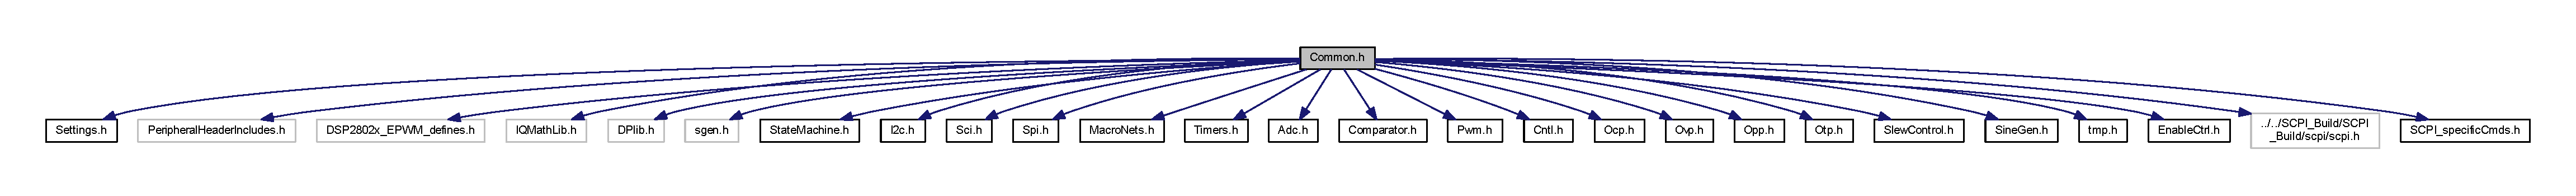
\includegraphics[width=350pt]{a00062}
\end{center}
\end{figure}


\subsection{Detailed Description}
Common include file for the project. All other header files used should be included within this file and this file should then be used to include them in the required source files. 
\hypertarget{a00017}{\section{Comparator.\-h File Reference}
\label{a00017}\index{Comparator.\-h@{Comparator.\-h}}
}


Comparator, D\-A\-C and trip zone functions.  


This graph shows which files directly or indirectly include this file\-:\nopagebreak
\begin{figure}[H]
\begin{center}
\leavevmode
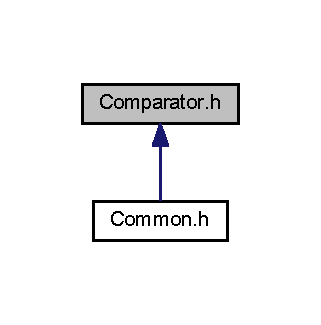
\includegraphics[width=154pt]{a00063}
\end{center}
\end{figure}
\subsection*{Functions}
\begin{DoxyCompactItemize}
\item 
void \hyperlink{a00017_a027da8e86de2dad92525a72406aca07b}{init\-Trip\-Zone} (void)
\item 
void \hyperlink{a00017_a7e69a8a85db8232ec6da973ef2861a5c}{init\-Dc\-Comparator} (void)
\item 
void \hyperlink{a00017_ae510122953eb2f6575eff63c4c0c6ae8}{rst\-Dc\-Tripzone} (void)
\item 
void \hyperlink{a00017_afac946d62f0f80d9c51a4e90a3b761a5}{init\-Ac\-Comparator} (void)
\item 
Uint16 \hyperlink{a00017_a4744ecd2e5380acd0df217952ca6db0d}{set\-Ac\-Dac} (float32 level)
\item 
Uint16 \hyperlink{a00017_a1d9a18a29a555d85f70597ff1d15c5de}{get\-Ac\-Dac} (float32 $\ast$level)
\item 
void \hyperlink{a00017_aa8b3c8342231e037104a6100df56b11b}{rst\-Ac\-Tripzone} (void)
\end{DoxyCompactItemize}


\subsection{Detailed Description}
Comparator, D\-A\-C and trip zone functions. Requires the modification of the C\-O\-M\-P\-\_\-\-R\-E\-G\-S struct of the D\-S\-P2802x\-\_\-\-Global\-Variable\-Defs in the file D\-S\-P2802x\-\_\-\-Comp.\-h, to allow use of the D\-A\-C\-C\-T\-L and ramp-\/related register unions. Use the equivalent file from the f2903x includes for reference. 

\subsection{Function Documentation}
\hypertarget{a00017_a1d9a18a29a555d85f70597ff1d15c5de}{\index{Comparator.\-h@{Comparator.\-h}!get\-Ac\-Dac@{get\-Ac\-Dac}}
\index{get\-Ac\-Dac@{get\-Ac\-Dac}!Comparator.h@{Comparator.\-h}}
\subsubsection[{get\-Ac\-Dac}]{\setlength{\rightskip}{0pt plus 5cm}Uint16 get\-Ac\-Dac (
\begin{DoxyParamCaption}
\item[{float32 $\ast$}]{level}
\end{DoxyParamCaption}
)}}\label{a00017_a1d9a18a29a555d85f70597ff1d15c5de}
Queries the output level setting of the D\-A\-C on the inverting input of the D\-C comparator. i\-Scale M\-U\-S\-T be set before use. 
\begin{DoxyParams}[1]{Parameters}
\mbox{\tt out}  & {\em level} & Pointer to location at which to place the query result (amps). \\
\hline
\end{DoxyParams}
\begin{DoxyReturn}{Returns}
Error status. 
\end{DoxyReturn}
\hypertarget{a00017_afac946d62f0f80d9c51a4e90a3b761a5}{\index{Comparator.\-h@{Comparator.\-h}!init\-Ac\-Comparator@{init\-Ac\-Comparator}}
\index{init\-Ac\-Comparator@{init\-Ac\-Comparator}!Comparator.h@{Comparator.\-h}}
\subsubsection[{init\-Ac\-Comparator}]{\setlength{\rightskip}{0pt plus 5cm}void init\-Ac\-Comparator (
\begin{DoxyParamCaption}
\item[{void}]{}
\end{DoxyParamCaption}
)}}\label{a00017_afac946d62f0f80d9c51a4e90a3b761a5}
Initialises the A\-C comparator (C\-O\-M\-P 1) using an internal D\-A\-C at the inverting input.
\begin{DoxyItemize}
\item S\-H\-O\-U\-L\-D be called A\-F\-T\-E\-R adc\-Soc\-Cnf().
\item S\-H\-O\-U\-L\-D be called B\-E\-F\-O\-R\-E P\-W\-M\-S (S\-Y\-N\-C) are started.
\item S\-H\-O\-U\-L\-D be called B\-E\-F\-O\-R\-E pwm\-T\-Z\-Configure(). 
\end{DoxyItemize}\hypertarget{a00017_a7e69a8a85db8232ec6da973ef2861a5c}{\index{Comparator.\-h@{Comparator.\-h}!init\-Dc\-Comparator@{init\-Dc\-Comparator}}
\index{init\-Dc\-Comparator@{init\-Dc\-Comparator}!Comparator.h@{Comparator.\-h}}
\subsubsection[{init\-Dc\-Comparator}]{\setlength{\rightskip}{0pt plus 5cm}void init\-Dc\-Comparator (
\begin{DoxyParamCaption}
\item[{void}]{}
\end{DoxyParamCaption}
)}}\label{a00017_a7e69a8a85db8232ec6da973ef2861a5c}
Initialises the D\-C comparator (C\-O\-M\-P 2) using an internal D\-A\-C at the inverting input.
\begin{DoxyItemize}
\item S\-H\-O\-U\-L\-D be called A\-F\-T\-E\-R adc\-Soc\-Cnf().
\item S\-H\-O\-U\-L\-D be called B\-E\-F\-O\-R\-E P\-W\-M\-S (S\-Y\-N\-C) are started.
\item S\-H\-O\-U\-L\-D be called B\-E\-F\-O\-R\-E pwm\-T\-Z\-Configure().
\item mid\-V\-Scale should be set before use. 
\end{DoxyItemize}\hypertarget{a00017_a027da8e86de2dad92525a72406aca07b}{\index{Comparator.\-h@{Comparator.\-h}!init\-Trip\-Zone@{init\-Trip\-Zone}}
\index{init\-Trip\-Zone@{init\-Trip\-Zone}!Comparator.h@{Comparator.\-h}}
\subsubsection[{init\-Trip\-Zone}]{\setlength{\rightskip}{0pt plus 5cm}void init\-Trip\-Zone (
\begin{DoxyParamCaption}
\item[{void}]{}
\end{DoxyParamCaption}
)}}\label{a00017_a027da8e86de2dad92525a72406aca07b}
Configures P\-W\-M trip zones for use. Requires the comparator and D\-A\-C to be configured \begin{DoxySeeAlso}{See Also}
\hyperlink{a00012}{adc.\-h} 
\end{DoxySeeAlso}
\hypertarget{a00017_aa8b3c8342231e037104a6100df56b11b}{\index{Comparator.\-h@{Comparator.\-h}!rst\-Ac\-Tripzone@{rst\-Ac\-Tripzone}}
\index{rst\-Ac\-Tripzone@{rst\-Ac\-Tripzone}!Comparator.h@{Comparator.\-h}}
\subsubsection[{rst\-Ac\-Tripzone}]{\setlength{\rightskip}{0pt plus 5cm}void rst\-Ac\-Tripzone (
\begin{DoxyParamCaption}
\item[{void}]{}
\end{DoxyParamCaption}
)}}\label{a00017_aa8b3c8342231e037104a6100df56b11b}
Resets the A\-C trip zone after an A\-C comparator event. \hypertarget{a00017_ae510122953eb2f6575eff63c4c0c6ae8}{\index{Comparator.\-h@{Comparator.\-h}!rst\-Dc\-Tripzone@{rst\-Dc\-Tripzone}}
\index{rst\-Dc\-Tripzone@{rst\-Dc\-Tripzone}!Comparator.h@{Comparator.\-h}}
\subsubsection[{rst\-Dc\-Tripzone}]{\setlength{\rightskip}{0pt plus 5cm}void rst\-Dc\-Tripzone (
\begin{DoxyParamCaption}
\item[{void}]{}
\end{DoxyParamCaption}
)}}\label{a00017_ae510122953eb2f6575eff63c4c0c6ae8}
Resets the D\-C trip zone after an D\-C comparator event. \hypertarget{a00017_a4744ecd2e5380acd0df217952ca6db0d}{\index{Comparator.\-h@{Comparator.\-h}!set\-Ac\-Dac@{set\-Ac\-Dac}}
\index{set\-Ac\-Dac@{set\-Ac\-Dac}!Comparator.h@{Comparator.\-h}}
\subsubsection[{set\-Ac\-Dac}]{\setlength{\rightskip}{0pt plus 5cm}Uint16 set\-Ac\-Dac (
\begin{DoxyParamCaption}
\item[{float32}]{level}
\end{DoxyParamCaption}
)}}\label{a00017_a4744ecd2e5380acd0df217952ca6db0d}
Sets the output level of the D\-A\-C on the inverting input of the A\-C comparator. The voltage and i\-Scale M\-U\-S\-T be set before use. 
\begin{DoxyParams}[1]{Parameters}
\mbox{\tt in}  & {\em level} & Specifies the value of the level setting to be applied (amps). \\
\hline
\end{DoxyParams}
\begin{DoxyReturn}{Returns}
Error status. 
\end{DoxyReturn}

\hypertarget{a00023}{\section{Enable\-Ctrl.\-h File Reference}
\label{a00023}\index{Enable\-Ctrl.\-h@{Enable\-Ctrl.\-h}}
}


Functions for enabling and disabling circuit sections via I2\-C.  


This graph shows which files directly or indirectly include this file\-:\nopagebreak
\begin{figure}[H]
\begin{center}
\leavevmode
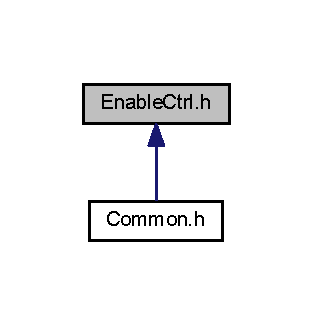
\includegraphics[width=150pt]{a00064}
\end{center}
\end{figure}
\subsection*{Macros}
\begin{DoxyCompactItemize}
\item 
\#define \hyperlink{a00023_a0cfe7137edc026282b36312077954701}{I\-O\-E\-\_\-\-S\-W4\-A\-\_\-\-S\-T\-A\-T\-E}~0x00
\item 
\#define \hyperlink{a00023_a5704aece7ac84dbd34e918fc0c60108d}{I\-O\-E\-\_\-\-S\-W4\-B\-\_\-\-S\-T\-A\-T\-E}~0x00
\item 
\#define \hyperlink{a00023_ab848e49bf7c4ea73e4ef05f26b3c60e8}{I\-O\-E\-\_\-\-I2\-C\-\_\-\-B\-A\-S\-E\-\_\-\-A\-D\-D\-R}~0x20
\item 
\#define \hyperlink{a00023_a36c134b088cc2e64e0a5e14e8f90fe38}{I\-O\-E\-\_\-\-I\-O\-D\-I\-R\-\_\-\-A\-D\-D\-R}~0x00
\item 
\#define \hyperlink{a00023_a04633cd2ea7fd0b332e1edf066f674c4}{I\-O\-E\-\_\-\-I\-P\-O\-L\-\_\-\-A\-D\-D\-R}~0x01
\item 
\#define \hyperlink{a00023_aa68be5a6ed28fb146600b4fd2d11fafd}{I\-O\-E\-\_\-\-G\-P\-I\-N\-T\-E\-N\-\_\-\-A\-D\-D\-R}~0x02
\item 
\#define \hyperlink{a00023_a687e15212e8d4b49c12159dce73eeeab}{I\-O\-E\-\_\-\-D\-E\-F\-V\-A\-L\-\_\-\-A\-D\-D\-R}~0x03
\item 
\#define \hyperlink{a00023_a90945d9544eebc892154f1e0443b1407}{I\-O\-E\-\_\-\-I\-N\-T\-C\-O\-N\-\_\-\-A\-D\-D\-R}~0x04
\item 
\#define \hyperlink{a00023_af44ed2bf93808aeb932ce9944a942b75}{I\-O\-E\-\_\-\-I\-O\-C\-O\-N\-\_\-\-A\-D\-D\-R}~0x05
\item 
\#define \hyperlink{a00023_a91e588d697383f94de2bf7f11d9ecb4b}{I\-O\-E\-\_\-\-G\-P\-P\-U\-\_\-\-A\-D\-D\-R}~0x06
\item 
\#define \hyperlink{a00023_a32cac2ad5af58a2562540ec8fc205dd1}{I\-O\-E\-\_\-\-I\-N\-T\-F\-\_\-\-A\-D\-D\-R}~0x07
\item 
\#define \hyperlink{a00023_ac0afd8503a8584599cc81f3d9b0a04dc}{I\-O\-E\-\_\-\-I\-N\-T\-C\-A\-P\-\_\-\-A\-D\-D\-R}~0x08
\item 
\#define \hyperlink{a00023_af2d85152c5775a221f107d6de547bca1}{I\-O\-E\-\_\-\-G\-P\-I\-O\-\_\-\-A\-D\-D\-R}~0x09
\item 
\#define \hyperlink{a00023_ab26864d7372ac11db9c1996842a3cf56}{I\-O\-E\-\_\-\-O\-L\-A\-T\-\_\-\-A\-D\-D\-R}~0x0\-A
\item 
\#define \hyperlink{a00023_a0ad928de8e88a9285e391d1c7b4a57c1}{I\-O\-E\-\_\-\-M\-A\-X\-\_\-\-C\-H\-N\-L}~0x08
\item 
\#define \hyperlink{a00023_ad615a329bea187ce779cf9930ba8a6fa}{I\-O\-E\-\_\-\-I2\-C\-\_\-\-A\-D\-D\-R}~(\hyperlink{a00023_ab848e49bf7c4ea73e4ef05f26b3c60e8}{I\-O\-E\-\_\-\-I2\-C\-\_\-\-B\-A\-S\-E\-\_\-\-A\-D\-D\-R} $|$ (\hyperlink{a00023_a0cfe7137edc026282b36312077954701}{I\-O\-E\-\_\-\-S\-W4\-A\-\_\-\-S\-T\-A\-T\-E} $<$$<$ 2)) $|$ (\hyperlink{a00023_a5704aece7ac84dbd34e918fc0c60108d}{I\-O\-E\-\_\-\-S\-W4\-B\-\_\-\-S\-T\-A\-T\-E} $<$$<$ 3)
\item 
\#define \hyperlink{a00023_a79846f375935e81b3781b88b40405d38}{A\-L\-L\-\_\-\-D\-I\-S\-A\-B\-L\-E\-D\-\_\-\-W\-O\-R\-D}
\end{DoxyCompactItemize}
\subsection*{Typedefs}
\begin{DoxyCompactItemize}
\item 
typedef enum \hyperlink{a00023_a693dd7ac614cd1a7f8bfd7440f34ed6f}{ec\-Section} \hyperlink{a00023_a5d2cb2e2fccefcdcb2e72e9e88b94223}{circuit\-Section}
\end{DoxyCompactItemize}
\subsection*{Enumerations}
\begin{DoxyCompactItemize}
\item 
enum \hyperlink{a00023_a693dd7ac614cd1a7f8bfd7440f34ed6f}{ec\-Section} 
\end{DoxyCompactItemize}
\subsection*{Functions}
\begin{DoxyCompactItemize}
\item 
Uint16 \hyperlink{a00023_ae6fd4f744738c8b2733ef36d92fb7313}{init\-Enable\-Control} (void)
\item 
void \hyperlink{a00023_a7e7f2b9153314c4652c5e0a1d2977133}{reset\-Enable\-Control} (void)
\item 
Uint16 \hyperlink{a00023_a5f4a447d1fbeba7920434b60e33b521e}{enable\-Circuit} (\hyperlink{a00023_a5d2cb2e2fccefcdcb2e72e9e88b94223}{circuit\-Section} section)
\item 
Uint16 \hyperlink{a00023_a606ff8e8b51f82c70ced419dad90f993}{disable\-Circuit} (\hyperlink{a00023_a5d2cb2e2fccefcdcb2e72e9e88b94223}{circuit\-Section} section)
\end{DoxyCompactItemize}


\subsection{Detailed Description}
Functions for enabling and disabling circuit sections via I2\-C. Circuit sections are controlled via an external I/\-O expander (M\-C\-P23008) that is connected to the I2\-C bus at address 0100xx0 where 'xx' is determined by the state of switch 4 (S\-W4) on the Ctrl P\-C\-B, which the user should record in the macros I\-O\-E\-\_\-\-S\-W4\-A\-\_\-\-S\-T\-A\-T\-E and I\-O\-E\-\_\-\-S\-W4\-B\-\_\-\-S\-T\-A\-T\-E.

After initialisation or reset all sections default to disabled.

\begin{DoxyWarning}{Warning}
Before any enable control functions can be used the I2\-C peripheral M\-U\-S\-T be initialised, followed by enable control initialisation, both of which will require global interrupts to be enabled.
\end{DoxyWarning}
\begin{DoxySeeAlso}{See Also}
\hyperlink{a00025_abcb138d5ddee570bf37734dde6ee291e}{init\-I2c()}
\end{DoxySeeAlso}
\begin{TabularC}{4}
\hline
\rowcolor{lightgray}\PBS\centering {\bf A\-D\-S7830 Ch \#}&\PBS\centering {\bf Signal }&\PBS\centering {\bf Enable bit\# }&\PBS\centering {\bf Enable state  }\\\cline{1-4}
\PBS\centering G\-P0 &\PBS\centering C\-H\-A\-N1\-E\-N &\PBS\centering 0 &\PBS\centering 1 \\\cline{1-4}
\PBS\centering G\-P1 &\PBS\centering C\-H\-A\-N2\-E\-N &\PBS\centering 1 &\PBS\centering 1 \\\cline{1-4}
\PBS\centering G\-P2 &\PBS\centering C\-H\-A\-N3\-E\-N &\PBS\centering 2 &\PBS\centering 1 \\\cline{1-4}
\PBS\centering G\-P3 &\PBS\centering C\-H\-A\-N4\-E\-N &\PBS\centering 3 &\PBS\centering 1 \\\cline{1-4}
\PBS\centering G\-P4 &\PBS\centering H\-V\-E\-N\-A\-B\-L\-E &\PBS\centering 4 &\PBS\centering 0 \\\cline{1-4}
\PBS\centering G\-P5 &\PBS\centering A\-C\-E\-N\-A\-B\-L\-E &\PBS\centering 5 &\PBS\centering 1 \\\cline{1-4}
\PBS\centering G\-P6 &\PBS\centering P\-S\-U\-E\-N\-B\-L\-E &\PBS\centering 6 &\PBS\centering 1 \\\cline{1-4}
\PBS\centering G\-P7 &\PBS\centering E\-X\-T\-F\-A\-N\-E\-N &\PBS\centering 7 &\PBS\centering 1 \\\cline{1-4}
\end{TabularC}


\subsection{Macro Definition Documentation}
\hypertarget{a00023_a79846f375935e81b3781b88b40405d38}{\index{Enable\-Ctrl.\-h@{Enable\-Ctrl.\-h}!A\-L\-L\-\_\-\-D\-I\-S\-A\-B\-L\-E\-D\-\_\-\-W\-O\-R\-D@{A\-L\-L\-\_\-\-D\-I\-S\-A\-B\-L\-E\-D\-\_\-\-W\-O\-R\-D}}
\index{A\-L\-L\-\_\-\-D\-I\-S\-A\-B\-L\-E\-D\-\_\-\-W\-O\-R\-D@{A\-L\-L\-\_\-\-D\-I\-S\-A\-B\-L\-E\-D\-\_\-\-W\-O\-R\-D}!EnableCtrl.h@{Enable\-Ctrl.\-h}}
\subsubsection[{A\-L\-L\-\_\-\-D\-I\-S\-A\-B\-L\-E\-D\-\_\-\-W\-O\-R\-D}]{\setlength{\rightskip}{0pt plus 5cm}\#define A\-L\-L\-\_\-\-D\-I\-S\-A\-B\-L\-E\-D\-\_\-\-W\-O\-R\-D}}\label{a00023_a79846f375935e81b3781b88b40405d38}
{\bfseries Value\-:}
\begin{DoxyCode}
(~(0 | (CHAN1\_EN\_STATE << chan1) | (CHAN2\_EN\_STATE << chan2) | (CHAN3\_EN\_STATE << chan3) \(\backslash\)
                               | (CHAN4\_EN\_STATE << chan4) | (XFMR\_EN\_STATE << xfmrCct) | (AC\_EN\_STATE << 
      acCct) \(\backslash\)
                               | (PSU\_EN\_STATE << psu) | (EXTFAN\_EN\_STATE << fan))) & 0x00FF
\end{DoxyCode}
Uses the defined states to define a word for the case where all circuits are disabled \hypertarget{a00023_a687e15212e8d4b49c12159dce73eeeab}{\index{Enable\-Ctrl.\-h@{Enable\-Ctrl.\-h}!I\-O\-E\-\_\-\-D\-E\-F\-V\-A\-L\-\_\-\-A\-D\-D\-R@{I\-O\-E\-\_\-\-D\-E\-F\-V\-A\-L\-\_\-\-A\-D\-D\-R}}
\index{I\-O\-E\-\_\-\-D\-E\-F\-V\-A\-L\-\_\-\-A\-D\-D\-R@{I\-O\-E\-\_\-\-D\-E\-F\-V\-A\-L\-\_\-\-A\-D\-D\-R}!EnableCtrl.h@{Enable\-Ctrl.\-h}}
\subsubsection[{I\-O\-E\-\_\-\-D\-E\-F\-V\-A\-L\-\_\-\-A\-D\-D\-R}]{\setlength{\rightskip}{0pt plus 5cm}\#define I\-O\-E\-\_\-\-D\-E\-F\-V\-A\-L\-\_\-\-A\-D\-D\-R~0x03}}\label{a00023_a687e15212e8d4b49c12159dce73eeeab}
M\-C\-P23008 I/\-O expander default value register address. \hypertarget{a00023_aa68be5a6ed28fb146600b4fd2d11fafd}{\index{Enable\-Ctrl.\-h@{Enable\-Ctrl.\-h}!I\-O\-E\-\_\-\-G\-P\-I\-N\-T\-E\-N\-\_\-\-A\-D\-D\-R@{I\-O\-E\-\_\-\-G\-P\-I\-N\-T\-E\-N\-\_\-\-A\-D\-D\-R}}
\index{I\-O\-E\-\_\-\-G\-P\-I\-N\-T\-E\-N\-\_\-\-A\-D\-D\-R@{I\-O\-E\-\_\-\-G\-P\-I\-N\-T\-E\-N\-\_\-\-A\-D\-D\-R}!EnableCtrl.h@{Enable\-Ctrl.\-h}}
\subsubsection[{I\-O\-E\-\_\-\-G\-P\-I\-N\-T\-E\-N\-\_\-\-A\-D\-D\-R}]{\setlength{\rightskip}{0pt plus 5cm}\#define I\-O\-E\-\_\-\-G\-P\-I\-N\-T\-E\-N\-\_\-\-A\-D\-D\-R~0x02}}\label{a00023_aa68be5a6ed28fb146600b4fd2d11fafd}
M\-C\-P23008 I/\-O expander interrupt on change enable register address. \hypertarget{a00023_af2d85152c5775a221f107d6de547bca1}{\index{Enable\-Ctrl.\-h@{Enable\-Ctrl.\-h}!I\-O\-E\-\_\-\-G\-P\-I\-O\-\_\-\-A\-D\-D\-R@{I\-O\-E\-\_\-\-G\-P\-I\-O\-\_\-\-A\-D\-D\-R}}
\index{I\-O\-E\-\_\-\-G\-P\-I\-O\-\_\-\-A\-D\-D\-R@{I\-O\-E\-\_\-\-G\-P\-I\-O\-\_\-\-A\-D\-D\-R}!EnableCtrl.h@{Enable\-Ctrl.\-h}}
\subsubsection[{I\-O\-E\-\_\-\-G\-P\-I\-O\-\_\-\-A\-D\-D\-R}]{\setlength{\rightskip}{0pt plus 5cm}\#define I\-O\-E\-\_\-\-G\-P\-I\-O\-\_\-\-A\-D\-D\-R~0x09}}\label{a00023_af2d85152c5775a221f107d6de547bca1}
M\-C\-P23008 I/\-O expander G\-P\-I\-O port register address. \hypertarget{a00023_a91e588d697383f94de2bf7f11d9ecb4b}{\index{Enable\-Ctrl.\-h@{Enable\-Ctrl.\-h}!I\-O\-E\-\_\-\-G\-P\-P\-U\-\_\-\-A\-D\-D\-R@{I\-O\-E\-\_\-\-G\-P\-P\-U\-\_\-\-A\-D\-D\-R}}
\index{I\-O\-E\-\_\-\-G\-P\-P\-U\-\_\-\-A\-D\-D\-R@{I\-O\-E\-\_\-\-G\-P\-P\-U\-\_\-\-A\-D\-D\-R}!EnableCtrl.h@{Enable\-Ctrl.\-h}}
\subsubsection[{I\-O\-E\-\_\-\-G\-P\-P\-U\-\_\-\-A\-D\-D\-R}]{\setlength{\rightskip}{0pt plus 5cm}\#define I\-O\-E\-\_\-\-G\-P\-P\-U\-\_\-\-A\-D\-D\-R~0x06}}\label{a00023_a91e588d697383f94de2bf7f11d9ecb4b}
M\-C\-P23008 I/\-O expander pull-\/up resistor configuration register address. \hypertarget{a00023_ad615a329bea187ce779cf9930ba8a6fa}{\index{Enable\-Ctrl.\-h@{Enable\-Ctrl.\-h}!I\-O\-E\-\_\-\-I2\-C\-\_\-\-A\-D\-D\-R@{I\-O\-E\-\_\-\-I2\-C\-\_\-\-A\-D\-D\-R}}
\index{I\-O\-E\-\_\-\-I2\-C\-\_\-\-A\-D\-D\-R@{I\-O\-E\-\_\-\-I2\-C\-\_\-\-A\-D\-D\-R}!EnableCtrl.h@{Enable\-Ctrl.\-h}}
\subsubsection[{I\-O\-E\-\_\-\-I2\-C\-\_\-\-A\-D\-D\-R}]{\setlength{\rightskip}{0pt plus 5cm}\#define I\-O\-E\-\_\-\-I2\-C\-\_\-\-A\-D\-D\-R~({\bf I\-O\-E\-\_\-\-I2\-C\-\_\-\-B\-A\-S\-E\-\_\-\-A\-D\-D\-R} $|$ ({\bf I\-O\-E\-\_\-\-S\-W4\-A\-\_\-\-S\-T\-A\-T\-E} $<$$<$ 2)) $|$ ({\bf I\-O\-E\-\_\-\-S\-W4\-B\-\_\-\-S\-T\-A\-T\-E} $<$$<$ 3)}}\label{a00023_ad615a329bea187ce779cf9930ba8a6fa}
M\-C\-P23008 I/\-O expander complete I2\-C address. \hypertarget{a00023_ab848e49bf7c4ea73e4ef05f26b3c60e8}{\index{Enable\-Ctrl.\-h@{Enable\-Ctrl.\-h}!I\-O\-E\-\_\-\-I2\-C\-\_\-\-B\-A\-S\-E\-\_\-\-A\-D\-D\-R@{I\-O\-E\-\_\-\-I2\-C\-\_\-\-B\-A\-S\-E\-\_\-\-A\-D\-D\-R}}
\index{I\-O\-E\-\_\-\-I2\-C\-\_\-\-B\-A\-S\-E\-\_\-\-A\-D\-D\-R@{I\-O\-E\-\_\-\-I2\-C\-\_\-\-B\-A\-S\-E\-\_\-\-A\-D\-D\-R}!EnableCtrl.h@{Enable\-Ctrl.\-h}}
\subsubsection[{I\-O\-E\-\_\-\-I2\-C\-\_\-\-B\-A\-S\-E\-\_\-\-A\-D\-D\-R}]{\setlength{\rightskip}{0pt plus 5cm}\#define I\-O\-E\-\_\-\-I2\-C\-\_\-\-B\-A\-S\-E\-\_\-\-A\-D\-D\-R~0x20}}\label{a00023_ab848e49bf7c4ea73e4ef05f26b3c60e8}
M\-C\-P23008 I/\-O expander base I2\-C address. \hypertarget{a00023_ac0afd8503a8584599cc81f3d9b0a04dc}{\index{Enable\-Ctrl.\-h@{Enable\-Ctrl.\-h}!I\-O\-E\-\_\-\-I\-N\-T\-C\-A\-P\-\_\-\-A\-D\-D\-R@{I\-O\-E\-\_\-\-I\-N\-T\-C\-A\-P\-\_\-\-A\-D\-D\-R}}
\index{I\-O\-E\-\_\-\-I\-N\-T\-C\-A\-P\-\_\-\-A\-D\-D\-R@{I\-O\-E\-\_\-\-I\-N\-T\-C\-A\-P\-\_\-\-A\-D\-D\-R}!EnableCtrl.h@{Enable\-Ctrl.\-h}}
\subsubsection[{I\-O\-E\-\_\-\-I\-N\-T\-C\-A\-P\-\_\-\-A\-D\-D\-R}]{\setlength{\rightskip}{0pt plus 5cm}\#define I\-O\-E\-\_\-\-I\-N\-T\-C\-A\-P\-\_\-\-A\-D\-D\-R~0x08}}\label{a00023_ac0afd8503a8584599cc81f3d9b0a04dc}
M\-C\-P23008 I/\-O expander interrupt capture register address. \hypertarget{a00023_a90945d9544eebc892154f1e0443b1407}{\index{Enable\-Ctrl.\-h@{Enable\-Ctrl.\-h}!I\-O\-E\-\_\-\-I\-N\-T\-C\-O\-N\-\_\-\-A\-D\-D\-R@{I\-O\-E\-\_\-\-I\-N\-T\-C\-O\-N\-\_\-\-A\-D\-D\-R}}
\index{I\-O\-E\-\_\-\-I\-N\-T\-C\-O\-N\-\_\-\-A\-D\-D\-R@{I\-O\-E\-\_\-\-I\-N\-T\-C\-O\-N\-\_\-\-A\-D\-D\-R}!EnableCtrl.h@{Enable\-Ctrl.\-h}}
\subsubsection[{I\-O\-E\-\_\-\-I\-N\-T\-C\-O\-N\-\_\-\-A\-D\-D\-R}]{\setlength{\rightskip}{0pt plus 5cm}\#define I\-O\-E\-\_\-\-I\-N\-T\-C\-O\-N\-\_\-\-A\-D\-D\-R~0x04}}\label{a00023_a90945d9544eebc892154f1e0443b1407}
M\-C\-P23008 I/\-O expander interrupt on change control register address. \hypertarget{a00023_a32cac2ad5af58a2562540ec8fc205dd1}{\index{Enable\-Ctrl.\-h@{Enable\-Ctrl.\-h}!I\-O\-E\-\_\-\-I\-N\-T\-F\-\_\-\-A\-D\-D\-R@{I\-O\-E\-\_\-\-I\-N\-T\-F\-\_\-\-A\-D\-D\-R}}
\index{I\-O\-E\-\_\-\-I\-N\-T\-F\-\_\-\-A\-D\-D\-R@{I\-O\-E\-\_\-\-I\-N\-T\-F\-\_\-\-A\-D\-D\-R}!EnableCtrl.h@{Enable\-Ctrl.\-h}}
\subsubsection[{I\-O\-E\-\_\-\-I\-N\-T\-F\-\_\-\-A\-D\-D\-R}]{\setlength{\rightskip}{0pt plus 5cm}\#define I\-O\-E\-\_\-\-I\-N\-T\-F\-\_\-\-A\-D\-D\-R~0x07}}\label{a00023_a32cac2ad5af58a2562540ec8fc205dd1}
M\-C\-P23008 I/\-O expander interrupt flag register address. \hypertarget{a00023_af44ed2bf93808aeb932ce9944a942b75}{\index{Enable\-Ctrl.\-h@{Enable\-Ctrl.\-h}!I\-O\-E\-\_\-\-I\-O\-C\-O\-N\-\_\-\-A\-D\-D\-R@{I\-O\-E\-\_\-\-I\-O\-C\-O\-N\-\_\-\-A\-D\-D\-R}}
\index{I\-O\-E\-\_\-\-I\-O\-C\-O\-N\-\_\-\-A\-D\-D\-R@{I\-O\-E\-\_\-\-I\-O\-C\-O\-N\-\_\-\-A\-D\-D\-R}!EnableCtrl.h@{Enable\-Ctrl.\-h}}
\subsubsection[{I\-O\-E\-\_\-\-I\-O\-C\-O\-N\-\_\-\-A\-D\-D\-R}]{\setlength{\rightskip}{0pt plus 5cm}\#define I\-O\-E\-\_\-\-I\-O\-C\-O\-N\-\_\-\-A\-D\-D\-R~0x05}}\label{a00023_af44ed2bf93808aeb932ce9944a942b75}
M\-C\-P23008 I/\-O expander configuration register address. \hypertarget{a00023_a36c134b088cc2e64e0a5e14e8f90fe38}{\index{Enable\-Ctrl.\-h@{Enable\-Ctrl.\-h}!I\-O\-E\-\_\-\-I\-O\-D\-I\-R\-\_\-\-A\-D\-D\-R@{I\-O\-E\-\_\-\-I\-O\-D\-I\-R\-\_\-\-A\-D\-D\-R}}
\index{I\-O\-E\-\_\-\-I\-O\-D\-I\-R\-\_\-\-A\-D\-D\-R@{I\-O\-E\-\_\-\-I\-O\-D\-I\-R\-\_\-\-A\-D\-D\-R}!EnableCtrl.h@{Enable\-Ctrl.\-h}}
\subsubsection[{I\-O\-E\-\_\-\-I\-O\-D\-I\-R\-\_\-\-A\-D\-D\-R}]{\setlength{\rightskip}{0pt plus 5cm}\#define I\-O\-E\-\_\-\-I\-O\-D\-I\-R\-\_\-\-A\-D\-D\-R~0x00}}\label{a00023_a36c134b088cc2e64e0a5e14e8f90fe38}
M\-C\-P23008 I/\-O expander I/\-O direction register address. \hypertarget{a00023_a04633cd2ea7fd0b332e1edf066f674c4}{\index{Enable\-Ctrl.\-h@{Enable\-Ctrl.\-h}!I\-O\-E\-\_\-\-I\-P\-O\-L\-\_\-\-A\-D\-D\-R@{I\-O\-E\-\_\-\-I\-P\-O\-L\-\_\-\-A\-D\-D\-R}}
\index{I\-O\-E\-\_\-\-I\-P\-O\-L\-\_\-\-A\-D\-D\-R@{I\-O\-E\-\_\-\-I\-P\-O\-L\-\_\-\-A\-D\-D\-R}!EnableCtrl.h@{Enable\-Ctrl.\-h}}
\subsubsection[{I\-O\-E\-\_\-\-I\-P\-O\-L\-\_\-\-A\-D\-D\-R}]{\setlength{\rightskip}{0pt plus 5cm}\#define I\-O\-E\-\_\-\-I\-P\-O\-L\-\_\-\-A\-D\-D\-R~0x01}}\label{a00023_a04633cd2ea7fd0b332e1edf066f674c4}
M\-C\-P23008 I/\-O expander input polarity register address. \hypertarget{a00023_a0ad928de8e88a9285e391d1c7b4a57c1}{\index{Enable\-Ctrl.\-h@{Enable\-Ctrl.\-h}!I\-O\-E\-\_\-\-M\-A\-X\-\_\-\-C\-H\-N\-L@{I\-O\-E\-\_\-\-M\-A\-X\-\_\-\-C\-H\-N\-L}}
\index{I\-O\-E\-\_\-\-M\-A\-X\-\_\-\-C\-H\-N\-L@{I\-O\-E\-\_\-\-M\-A\-X\-\_\-\-C\-H\-N\-L}!EnableCtrl.h@{Enable\-Ctrl.\-h}}
\subsubsection[{I\-O\-E\-\_\-\-M\-A\-X\-\_\-\-C\-H\-N\-L}]{\setlength{\rightskip}{0pt plus 5cm}\#define I\-O\-E\-\_\-\-M\-A\-X\-\_\-\-C\-H\-N\-L~0x08}}\label{a00023_a0ad928de8e88a9285e391d1c7b4a57c1}
M\-C\-P23008 I/\-O expander number of channels (0 -\/ 7). \hypertarget{a00023_ab26864d7372ac11db9c1996842a3cf56}{\index{Enable\-Ctrl.\-h@{Enable\-Ctrl.\-h}!I\-O\-E\-\_\-\-O\-L\-A\-T\-\_\-\-A\-D\-D\-R@{I\-O\-E\-\_\-\-O\-L\-A\-T\-\_\-\-A\-D\-D\-R}}
\index{I\-O\-E\-\_\-\-O\-L\-A\-T\-\_\-\-A\-D\-D\-R@{I\-O\-E\-\_\-\-O\-L\-A\-T\-\_\-\-A\-D\-D\-R}!EnableCtrl.h@{Enable\-Ctrl.\-h}}
\subsubsection[{I\-O\-E\-\_\-\-O\-L\-A\-T\-\_\-\-A\-D\-D\-R}]{\setlength{\rightskip}{0pt plus 5cm}\#define I\-O\-E\-\_\-\-O\-L\-A\-T\-\_\-\-A\-D\-D\-R~0x0\-A}}\label{a00023_ab26864d7372ac11db9c1996842a3cf56}
M\-C\-P23008 I/\-O expander output latch register address. \hypertarget{a00023_a0cfe7137edc026282b36312077954701}{\index{Enable\-Ctrl.\-h@{Enable\-Ctrl.\-h}!I\-O\-E\-\_\-\-S\-W4\-A\-\_\-\-S\-T\-A\-T\-E@{I\-O\-E\-\_\-\-S\-W4\-A\-\_\-\-S\-T\-A\-T\-E}}
\index{I\-O\-E\-\_\-\-S\-W4\-A\-\_\-\-S\-T\-A\-T\-E@{I\-O\-E\-\_\-\-S\-W4\-A\-\_\-\-S\-T\-A\-T\-E}!EnableCtrl.h@{Enable\-Ctrl.\-h}}
\subsubsection[{I\-O\-E\-\_\-\-S\-W4\-A\-\_\-\-S\-T\-A\-T\-E}]{\setlength{\rightskip}{0pt plus 5cm}\#define I\-O\-E\-\_\-\-S\-W4\-A\-\_\-\-S\-T\-A\-T\-E~0x00}}\label{a00023_a0cfe7137edc026282b36312077954701}
The state of switch 4a; O\-N = 0x01, O\-F\-F = 0x00. \hypertarget{a00023_a5704aece7ac84dbd34e918fc0c60108d}{\index{Enable\-Ctrl.\-h@{Enable\-Ctrl.\-h}!I\-O\-E\-\_\-\-S\-W4\-B\-\_\-\-S\-T\-A\-T\-E@{I\-O\-E\-\_\-\-S\-W4\-B\-\_\-\-S\-T\-A\-T\-E}}
\index{I\-O\-E\-\_\-\-S\-W4\-B\-\_\-\-S\-T\-A\-T\-E@{I\-O\-E\-\_\-\-S\-W4\-B\-\_\-\-S\-T\-A\-T\-E}!EnableCtrl.h@{Enable\-Ctrl.\-h}}
\subsubsection[{I\-O\-E\-\_\-\-S\-W4\-B\-\_\-\-S\-T\-A\-T\-E}]{\setlength{\rightskip}{0pt plus 5cm}\#define I\-O\-E\-\_\-\-S\-W4\-B\-\_\-\-S\-T\-A\-T\-E~0x00}}\label{a00023_a5704aece7ac84dbd34e918fc0c60108d}
The state of switch 4b; O\-N = 0x01, O\-F\-F = 0x00. 

\subsection{Typedef Documentation}
\hypertarget{a00023_a5d2cb2e2fccefcdcb2e72e9e88b94223}{\index{Enable\-Ctrl.\-h@{Enable\-Ctrl.\-h}!circuit\-Section@{circuit\-Section}}
\index{circuit\-Section@{circuit\-Section}!EnableCtrl.h@{Enable\-Ctrl.\-h}}
\subsubsection[{circuit\-Section}]{\setlength{\rightskip}{0pt plus 5cm}typedef enum {\bf ec\-Section} {\bf circuit\-Section}}}\label{a00023_a5d2cb2e2fccefcdcb2e72e9e88b94223}
A type that allow specification of an enable control circuit section. 

\subsection{Enumeration Type Documentation}
\hypertarget{a00023_a693dd7ac614cd1a7f8bfd7440f34ed6f}{\index{Enable\-Ctrl.\-h@{Enable\-Ctrl.\-h}!ec\-Section@{ec\-Section}}
\index{ec\-Section@{ec\-Section}!EnableCtrl.h@{Enable\-Ctrl.\-h}}
\subsubsection[{ec\-Section}]{\setlength{\rightskip}{0pt plus 5cm}enum {\bf ec\-Section}}}\label{a00023_a693dd7ac614cd1a7f8bfd7440f34ed6f}
The possible enable control circuit section selections. Also defines bit order. 

\subsection{Function Documentation}
\hypertarget{a00023_a606ff8e8b51f82c70ced419dad90f993}{\index{Enable\-Ctrl.\-h@{Enable\-Ctrl.\-h}!disable\-Circuit@{disable\-Circuit}}
\index{disable\-Circuit@{disable\-Circuit}!EnableCtrl.h@{Enable\-Ctrl.\-h}}
\subsubsection[{disable\-Circuit}]{\setlength{\rightskip}{0pt plus 5cm}Uint16 disable\-Circuit (
\begin{DoxyParamCaption}
\item[{{\bf circuit\-Section}}]{section}
\end{DoxyParamCaption}
)}}\label{a00023_a606ff8e8b51f82c70ced419dad90f993}
Disables the specified circuit section enable signal. 
\begin{DoxyParams}[1]{Parameters}
\mbox{\tt in}  & {\em section} & Specifies the circuit section that is to be disabled. \\
\hline
\end{DoxyParams}
\begin{DoxyReturn}{Returns}
Error status. 
\end{DoxyReturn}
\hypertarget{a00023_a5f4a447d1fbeba7920434b60e33b521e}{\index{Enable\-Ctrl.\-h@{Enable\-Ctrl.\-h}!enable\-Circuit@{enable\-Circuit}}
\index{enable\-Circuit@{enable\-Circuit}!EnableCtrl.h@{Enable\-Ctrl.\-h}}
\subsubsection[{enable\-Circuit}]{\setlength{\rightskip}{0pt plus 5cm}Uint16 enable\-Circuit (
\begin{DoxyParamCaption}
\item[{{\bf circuit\-Section}}]{section}
\end{DoxyParamCaption}
)}}\label{a00023_a5f4a447d1fbeba7920434b60e33b521e}
Enables the specified circuit section enable signal. 
\begin{DoxyParams}[1]{Parameters}
\mbox{\tt in}  & {\em section} & Specifies the circuit section that is to be enabled. \\
\hline
\end{DoxyParams}
\begin{DoxyReturn}{Returns}
Error status. 
\end{DoxyReturn}
\hypertarget{a00023_ae6fd4f744738c8b2733ef36d92fb7313}{\index{Enable\-Ctrl.\-h@{Enable\-Ctrl.\-h}!init\-Enable\-Control@{init\-Enable\-Control}}
\index{init\-Enable\-Control@{init\-Enable\-Control}!EnableCtrl.h@{Enable\-Ctrl.\-h}}
\subsubsection[{init\-Enable\-Control}]{\setlength{\rightskip}{0pt plus 5cm}Uint16 init\-Enable\-Control (
\begin{DoxyParamCaption}
\item[{void}]{}
\end{DoxyParamCaption}
)}}\label{a00023_ae6fd4f744738c8b2733ef36d92fb7313}
Initialises the enable control interface. The I2\-C peripheral M\-U\-S\-T be initialised before this function is used. \begin{DoxySeeAlso}{See Also}
i2c\-Init() 
\end{DoxySeeAlso}
\begin{DoxyReturn}{Returns}
Error status. 
\end{DoxyReturn}
\hypertarget{a00023_a7e7f2b9153314c4652c5e0a1d2977133}{\index{Enable\-Ctrl.\-h@{Enable\-Ctrl.\-h}!reset\-Enable\-Control@{reset\-Enable\-Control}}
\index{reset\-Enable\-Control@{reset\-Enable\-Control}!EnableCtrl.h@{Enable\-Ctrl.\-h}}
\subsubsection[{reset\-Enable\-Control}]{\setlength{\rightskip}{0pt plus 5cm}void reset\-Enable\-Control (
\begin{DoxyParamCaption}
\item[{void}]{}
\end{DoxyParamCaption}
)}}\label{a00023_a7e7f2b9153314c4652c5e0a1d2977133}
Resets and reinitialises the M\-C\-P23008 I/\-O Expander device. 
\hypertarget{a00025}{\section{I2c.\-h File Reference}
\label{a00025}\index{I2c.\-h@{I2c.\-h}}
}


Inter-\/integrated circuit communications functions.  


This graph shows which files directly or indirectly include this file\-:\nopagebreak
\begin{figure}[H]
\begin{center}
\leavevmode
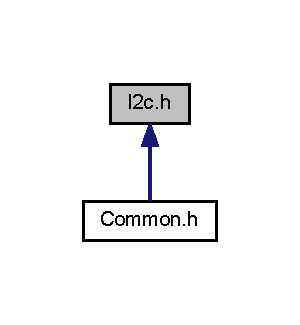
\includegraphics[width=144pt]{a00065}
\end{center}
\end{figure}
\subsection*{Data Structures}
\begin{DoxyCompactItemize}
\item 
struct \hyperlink{a00006}{i2c\-Msg}
\end{DoxyCompactItemize}
\subsection*{Macros}
\begin{DoxyCompactItemize}
\item 
\#define \hyperlink{a00025_a0889ccb6e4a98d6d8a0bf7c009c818e2}{I2\-C\-\_\-\-M\-A\-X\-\_\-\-B\-U\-F\-F\-E\-R\-\_\-\-S\-I\-Z\-E}~0x04
\item 
\#define \hyperlink{a00025_ae429af928d46f8186343fb3eb550dc92}{I2\-C\-\_\-\-M\-A\-X\-\_\-\-P\-T\-R\-\_\-\-S\-I\-Z\-E}~0x02
\end{DoxyCompactItemize}
{\bf }\par
\begin{DoxyCompactItemize}
\item 
\#define \hyperlink{a00025_a8e07057d8bd0732259c8b4aba0ccf747}{I2\-C\-\_\-\-C\-L\-R\-\_\-\-A\-L\-\_\-\-B\-I\-T}~0x0001
\item 
\#define \hyperlink{a00025_ac28843bc51cce0ce461810ff06c1dddc}{I2\-C\-\_\-\-C\-L\-R\-\_\-\-N\-A\-C\-K\-\_\-\-B\-I\-T}~0x0002
\item 
\#define \hyperlink{a00025_a4496263a3b781866a48a6b7e8fcc1543}{I2\-C\-\_\-\-C\-L\-R\-\_\-\-A\-R\-D\-Y\-\_\-\-B\-I\-T}~0x0004
\item 
\#define \hyperlink{a00025_a10317717bb3efb7ede2a49999fd161ba}{I2\-C\-\_\-\-C\-L\-R\-\_\-\-R\-R\-D\-Y\-\_\-\-B\-I\-T}~0x0008
\item 
\#define \hyperlink{a00025_aeb930d2f95f82d333b27b02f9586c3cd}{I2\-C\-\_\-\-C\-L\-R\-\_\-\-S\-C\-D\-\_\-\-B\-I\-T}~0x0020
\end{DoxyCompactItemize}

{\bf }\par
\begin{DoxyCompactItemize}
\item 
\#define \hyperlink{a00025_adf7bc6e4d458e0b13f0ad26570f04528}{I2\-C\-\_\-\-A\-R\-D\-Y\-\_\-\-I\-S\-R\-C}~0x0003
\item 
\#define \hyperlink{a00025_aa26238e86d534cda62318e98e1655654}{I2\-C\-\_\-\-S\-C\-D\-\_\-\-I\-S\-R\-C}~0x0006
\end{DoxyCompactItemize}

{\bf }\par
\begin{DoxyCompactItemize}
\item 
\#define \hyperlink{a00025_ad7ff7f3ddb5fb35b633d558b376cf329}{I2\-C\-\_\-\-M\-S\-G\-S\-T\-A\-T\-\_\-\-I\-N\-A\-C\-T\-I\-V\-E}~0x0000
\item 
\#define \hyperlink{a00025_a56f7eeab5c8dbbe042a10d1f8ac1ad55}{I2\-C\-\_\-\-M\-S\-G\-S\-T\-A\-T\-\_\-\-S\-E\-N\-D\-\_\-\-W\-I\-T\-H\-S\-T\-O\-P}~0x0010
\item 
\#define \hyperlink{a00025_a36809495e97c0e8033246b227f9716be}{I2\-C\-\_\-\-M\-S\-G\-S\-T\-A\-T\-\_\-\-W\-R\-I\-T\-E\-\_\-\-B\-U\-S\-Y}~0x0011
\item 
\#define \hyperlink{a00025_a6b46589e75a5bfdc3c57b0bc30cc8671}{I2\-C\-\_\-\-M\-S\-G\-S\-T\-A\-T\-\_\-\-S\-E\-N\-D\-\_\-\-N\-O\-S\-T\-O\-P}~0x0020
\item 
\#define \hyperlink{a00025_adbe18b39fde045ed6d51eaa7e17b78e0}{I2\-C\-\_\-\-M\-S\-G\-S\-T\-A\-T\-\_\-\-S\-E\-N\-D\-\_\-\-N\-O\-S\-T\-O\-P\-\_\-\-B\-U\-S\-Y}~0x0021
\item 
\#define \hyperlink{a00025_adf5a3e5950b5af97d3ec2e40b96c2251}{I2\-C\-\_\-\-M\-S\-G\-S\-T\-A\-T\-\_\-\-R\-E\-S\-T\-A\-R\-T}~0x0022
\item 
\#define \hyperlink{a00025_a9bd9503fa86f5b4d52aeb21be008064a}{I2\-C\-\_\-\-M\-S\-G\-S\-T\-A\-T\-\_\-\-R\-E\-A\-D\-\_\-\-B\-U\-S\-Y}~0x0023
\end{DoxyCompactItemize}

\subsection*{Functions}
\begin{DoxyCompactItemize}
\item 
void \hyperlink{a00025_abcb138d5ddee570bf37734dde6ee291e}{init\-I2c} (void)
\item 
void \hyperlink{a00025_a9e3198d675e7b65c3652bb5c887a7a64}{i2c\-Pop\-Msg} (\hyperlink{a00006}{i2c\-Msg} $\ast$msg, Uint16 msg\-Status, Uint16 slave\-Addr, Uint16 num\-Data\-Bytes, Uint16 num\-Slave\-Ptr\-Bytes, Uint16 slave\-Ptr\-Addr\-Hi, Uint16 slave\-Ptr\-Addr\-Lo)
\item 
Uint16 \hyperlink{a00025_a3813bb8cae6159f7df2672a55be4014b}{i2c\-Write} (\hyperlink{a00006}{i2c\-Msg} $\ast$msg)
\item 
Uint16 \hyperlink{a00025_aa681ec1b6413dd7009a6aaf0df2cbac1}{i2c\-Read} (\hyperlink{a00006}{i2c\-Msg} $\ast$msg)
\end{DoxyCompactItemize}


\subsection{Detailed Description}
Inter-\/integrated circuit communications functions. \begin{DoxyWarning}{Warning}
The following bridge tracks should be cut on the T\-I C2000 Launch\-Pad X\-L P\-C\-B before I2\-C (or S\-P\-I) may be used\-: \begin{TabularC}{3}
\hline
\rowcolor{lightgray}\PBS\centering {\bf Bridge to Cut }&\PBS\centering {\bf G\-P\-I\-O }&\PBS\centering {\bf P\-C\-B Pin  }\\\cline{1-3}
\PBS\centering J\-P5 &\PBS\centering G\-P\-I\-O32&\PBS\centering J2-\/6 \\\cline{1-3}
\PBS\centering J\-P7 &\PBS\centering G\-P\-I\-O33&\PBS\centering J2-\/7 \\\cline{1-3}
\PBS\centering J\-P8 &\PBS\centering G\-P\-I\-O16&\PBS\centering J6-\/7 \\\cline{1-3}
\PBS\centering J\-P10 &\PBS\centering G\-P\-I\-O17&\PBS\centering J6-\/8 \\\cline{1-3}
\end{TabularC}
This should result in the following functionality\-: \begin{TabularC}{3}
\hline
\rowcolor{lightgray}\PBS\centering {\bf Function }&\PBS\centering {\bf G\-P\-I\-O }&\PBS\centering {\bf P\-C\-B Pin  }\\\cline{1-3}
\PBS\centering I2\-C\-\_\-\-S\-D\-A\-A &\PBS\centering G\-P\-I\-O32&\PBS\centering J6-\/7 \\\cline{1-3}
\PBS\centering I2\-C\-\_\-\-S\-C\-L\-A &\PBS\centering G\-P\-I\-O33&\PBS\centering J6-\/8 \\\cline{1-3}
\PBS\centering S\-P\-I\-\_\-\-M\-O\-S\-I &\PBS\centering G\-P\-I\-O16&\PBS\centering J2-\/6 \\\cline{1-3}
\PBS\centering S\-P\-I\-\_\-\-M\-I\-S\-O &\PBS\centering G\-P\-I\-O17&\PBS\centering J2-\/7 \\\cline{1-3}
\end{TabularC}


The function i2c\-Init() M\-U\-S\-T be called before any other public I2\-C function is used. This will clear any values already in the I2\-C registers.

Interrupts M\-U\-S\-T be globally enabled for the functions \hyperlink{a00025_a3813bb8cae6159f7df2672a55be4014b}{i2c\-Write()} and \hyperlink{a00025_aa681ec1b6413dd7009a6aaf0df2cbac1}{i2c\-Read()} to operate correctly.
\end{DoxyWarning}
\begin{DoxySeeAlso}{See Also}
\hyperlink{a00023}{Enable\-Ctrl.\-h} 

\hyperlink{a00058}{Tmp.\-h} 
\end{DoxySeeAlso}


\subsection{Macro Definition Documentation}
\hypertarget{a00025_adf7bc6e4d458e0b13f0ad26570f04528}{\index{I2c.\-h@{I2c.\-h}!I2\-C\-\_\-\-A\-R\-D\-Y\-\_\-\-I\-S\-R\-C@{I2\-C\-\_\-\-A\-R\-D\-Y\-\_\-\-I\-S\-R\-C}}
\index{I2\-C\-\_\-\-A\-R\-D\-Y\-\_\-\-I\-S\-R\-C@{I2\-C\-\_\-\-A\-R\-D\-Y\-\_\-\-I\-S\-R\-C}!I2c.h@{I2c.\-h}}
\subsubsection[{I2\-C\-\_\-\-A\-R\-D\-Y\-\_\-\-I\-S\-R\-C}]{\setlength{\rightskip}{0pt plus 5cm}\#define I2\-C\-\_\-\-A\-R\-D\-Y\-\_\-\-I\-S\-R\-C~0x0003}}\label{a00025_adf7bc6e4d458e0b13f0ad26570f04528}
I2\-C Interrupt Sources Register access ready condition I2\-C interrupt source. \hypertarget{a00025_a8e07057d8bd0732259c8b4aba0ccf747}{\index{I2c.\-h@{I2c.\-h}!I2\-C\-\_\-\-C\-L\-R\-\_\-\-A\-L\-\_\-\-B\-I\-T@{I2\-C\-\_\-\-C\-L\-R\-\_\-\-A\-L\-\_\-\-B\-I\-T}}
\index{I2\-C\-\_\-\-C\-L\-R\-\_\-\-A\-L\-\_\-\-B\-I\-T@{I2\-C\-\_\-\-C\-L\-R\-\_\-\-A\-L\-\_\-\-B\-I\-T}!I2c.h@{I2c.\-h}}
\subsubsection[{I2\-C\-\_\-\-C\-L\-R\-\_\-\-A\-L\-\_\-\-B\-I\-T}]{\setlength{\rightskip}{0pt plus 5cm}\#define I2\-C\-\_\-\-C\-L\-R\-\_\-\-A\-L\-\_\-\-B\-I\-T~0x0001}}\label{a00025_a8e07057d8bd0732259c8b4aba0ccf747}
I2\-C Status Clear Bits Arbitration lost status clear bit. \hypertarget{a00025_a4496263a3b781866a48a6b7e8fcc1543}{\index{I2c.\-h@{I2c.\-h}!I2\-C\-\_\-\-C\-L\-R\-\_\-\-A\-R\-D\-Y\-\_\-\-B\-I\-T@{I2\-C\-\_\-\-C\-L\-R\-\_\-\-A\-R\-D\-Y\-\_\-\-B\-I\-T}}
\index{I2\-C\-\_\-\-C\-L\-R\-\_\-\-A\-R\-D\-Y\-\_\-\-B\-I\-T@{I2\-C\-\_\-\-C\-L\-R\-\_\-\-A\-R\-D\-Y\-\_\-\-B\-I\-T}!I2c.h@{I2c.\-h}}
\subsubsection[{I2\-C\-\_\-\-C\-L\-R\-\_\-\-A\-R\-D\-Y\-\_\-\-B\-I\-T}]{\setlength{\rightskip}{0pt plus 5cm}\#define I2\-C\-\_\-\-C\-L\-R\-\_\-\-A\-R\-D\-Y\-\_\-\-B\-I\-T~0x0004}}\label{a00025_a4496263a3b781866a48a6b7e8fcc1543}
Register access ready status clear bit. \hypertarget{a00025_ac28843bc51cce0ce461810ff06c1dddc}{\index{I2c.\-h@{I2c.\-h}!I2\-C\-\_\-\-C\-L\-R\-\_\-\-N\-A\-C\-K\-\_\-\-B\-I\-T@{I2\-C\-\_\-\-C\-L\-R\-\_\-\-N\-A\-C\-K\-\_\-\-B\-I\-T}}
\index{I2\-C\-\_\-\-C\-L\-R\-\_\-\-N\-A\-C\-K\-\_\-\-B\-I\-T@{I2\-C\-\_\-\-C\-L\-R\-\_\-\-N\-A\-C\-K\-\_\-\-B\-I\-T}!I2c.h@{I2c.\-h}}
\subsubsection[{I2\-C\-\_\-\-C\-L\-R\-\_\-\-N\-A\-C\-K\-\_\-\-B\-I\-T}]{\setlength{\rightskip}{0pt plus 5cm}\#define I2\-C\-\_\-\-C\-L\-R\-\_\-\-N\-A\-C\-K\-\_\-\-B\-I\-T~0x0002}}\label{a00025_ac28843bc51cce0ce461810ff06c1dddc}
N\-A\-C\-K status clear bit. \hypertarget{a00025_a10317717bb3efb7ede2a49999fd161ba}{\index{I2c.\-h@{I2c.\-h}!I2\-C\-\_\-\-C\-L\-R\-\_\-\-R\-R\-D\-Y\-\_\-\-B\-I\-T@{I2\-C\-\_\-\-C\-L\-R\-\_\-\-R\-R\-D\-Y\-\_\-\-B\-I\-T}}
\index{I2\-C\-\_\-\-C\-L\-R\-\_\-\-R\-R\-D\-Y\-\_\-\-B\-I\-T@{I2\-C\-\_\-\-C\-L\-R\-\_\-\-R\-R\-D\-Y\-\_\-\-B\-I\-T}!I2c.h@{I2c.\-h}}
\subsubsection[{I2\-C\-\_\-\-C\-L\-R\-\_\-\-R\-R\-D\-Y\-\_\-\-B\-I\-T}]{\setlength{\rightskip}{0pt plus 5cm}\#define I2\-C\-\_\-\-C\-L\-R\-\_\-\-R\-R\-D\-Y\-\_\-\-B\-I\-T~0x0008}}\label{a00025_a10317717bb3efb7ede2a49999fd161ba}
Receive data ready status clear bit. \hypertarget{a00025_aeb930d2f95f82d333b27b02f9586c3cd}{\index{I2c.\-h@{I2c.\-h}!I2\-C\-\_\-\-C\-L\-R\-\_\-\-S\-C\-D\-\_\-\-B\-I\-T@{I2\-C\-\_\-\-C\-L\-R\-\_\-\-S\-C\-D\-\_\-\-B\-I\-T}}
\index{I2\-C\-\_\-\-C\-L\-R\-\_\-\-S\-C\-D\-\_\-\-B\-I\-T@{I2\-C\-\_\-\-C\-L\-R\-\_\-\-S\-C\-D\-\_\-\-B\-I\-T}!I2c.h@{I2c.\-h}}
\subsubsection[{I2\-C\-\_\-\-C\-L\-R\-\_\-\-S\-C\-D\-\_\-\-B\-I\-T}]{\setlength{\rightskip}{0pt plus 5cm}\#define I2\-C\-\_\-\-C\-L\-R\-\_\-\-S\-C\-D\-\_\-\-B\-I\-T~0x0020}}\label{a00025_aeb930d2f95f82d333b27b02f9586c3cd}
Stop detected status clear bit. \hypertarget{a00025_a0889ccb6e4a98d6d8a0bf7c009c818e2}{\index{I2c.\-h@{I2c.\-h}!I2\-C\-\_\-\-M\-A\-X\-\_\-\-B\-U\-F\-F\-E\-R\-\_\-\-S\-I\-Z\-E@{I2\-C\-\_\-\-M\-A\-X\-\_\-\-B\-U\-F\-F\-E\-R\-\_\-\-S\-I\-Z\-E}}
\index{I2\-C\-\_\-\-M\-A\-X\-\_\-\-B\-U\-F\-F\-E\-R\-\_\-\-S\-I\-Z\-E@{I2\-C\-\_\-\-M\-A\-X\-\_\-\-B\-U\-F\-F\-E\-R\-\_\-\-S\-I\-Z\-E}!I2c.h@{I2c.\-h}}
\subsubsection[{I2\-C\-\_\-\-M\-A\-X\-\_\-\-B\-U\-F\-F\-E\-R\-\_\-\-S\-I\-Z\-E}]{\setlength{\rightskip}{0pt plus 5cm}\#define I2\-C\-\_\-\-M\-A\-X\-\_\-\-B\-U\-F\-F\-E\-R\-\_\-\-S\-I\-Z\-E~0x04}}\label{a00025_a0889ccb6e4a98d6d8a0bf7c009c818e2}
Maximum I2\-C message buffer size in bytes, including slave register pointer bytes. \hypertarget{a00025_ae429af928d46f8186343fb3eb550dc92}{\index{I2c.\-h@{I2c.\-h}!I2\-C\-\_\-\-M\-A\-X\-\_\-\-P\-T\-R\-\_\-\-S\-I\-Z\-E@{I2\-C\-\_\-\-M\-A\-X\-\_\-\-P\-T\-R\-\_\-\-S\-I\-Z\-E}}
\index{I2\-C\-\_\-\-M\-A\-X\-\_\-\-P\-T\-R\-\_\-\-S\-I\-Z\-E@{I2\-C\-\_\-\-M\-A\-X\-\_\-\-P\-T\-R\-\_\-\-S\-I\-Z\-E}!I2c.h@{I2c.\-h}}
\subsubsection[{I2\-C\-\_\-\-M\-A\-X\-\_\-\-P\-T\-R\-\_\-\-S\-I\-Z\-E}]{\setlength{\rightskip}{0pt plus 5cm}\#define I2\-C\-\_\-\-M\-A\-X\-\_\-\-P\-T\-R\-\_\-\-S\-I\-Z\-E~0x02}}\label{a00025_ae429af928d46f8186343fb3eb550dc92}
Maximum number of slave register pointer bytes. \hypertarget{a00025_ad7ff7f3ddb5fb35b633d558b376cf329}{\index{I2c.\-h@{I2c.\-h}!I2\-C\-\_\-\-M\-S\-G\-S\-T\-A\-T\-\_\-\-I\-N\-A\-C\-T\-I\-V\-E@{I2\-C\-\_\-\-M\-S\-G\-S\-T\-A\-T\-\_\-\-I\-N\-A\-C\-T\-I\-V\-E}}
\index{I2\-C\-\_\-\-M\-S\-G\-S\-T\-A\-T\-\_\-\-I\-N\-A\-C\-T\-I\-V\-E@{I2\-C\-\_\-\-M\-S\-G\-S\-T\-A\-T\-\_\-\-I\-N\-A\-C\-T\-I\-V\-E}!I2c.h@{I2c.\-h}}
\subsubsection[{I2\-C\-\_\-\-M\-S\-G\-S\-T\-A\-T\-\_\-\-I\-N\-A\-C\-T\-I\-V\-E}]{\setlength{\rightskip}{0pt plus 5cm}\#define I2\-C\-\_\-\-M\-S\-G\-S\-T\-A\-T\-\_\-\-I\-N\-A\-C\-T\-I\-V\-E~0x0000}}\label{a00025_ad7ff7f3ddb5fb35b633d558b376cf329}
I2\-C Message States Inactive I2\-C message state. \hypertarget{a00025_a9bd9503fa86f5b4d52aeb21be008064a}{\index{I2c.\-h@{I2c.\-h}!I2\-C\-\_\-\-M\-S\-G\-S\-T\-A\-T\-\_\-\-R\-E\-A\-D\-\_\-\-B\-U\-S\-Y@{I2\-C\-\_\-\-M\-S\-G\-S\-T\-A\-T\-\_\-\-R\-E\-A\-D\-\_\-\-B\-U\-S\-Y}}
\index{I2\-C\-\_\-\-M\-S\-G\-S\-T\-A\-T\-\_\-\-R\-E\-A\-D\-\_\-\-B\-U\-S\-Y@{I2\-C\-\_\-\-M\-S\-G\-S\-T\-A\-T\-\_\-\-R\-E\-A\-D\-\_\-\-B\-U\-S\-Y}!I2c.h@{I2c.\-h}}
\subsubsection[{I2\-C\-\_\-\-M\-S\-G\-S\-T\-A\-T\-\_\-\-R\-E\-A\-D\-\_\-\-B\-U\-S\-Y}]{\setlength{\rightskip}{0pt plus 5cm}\#define I2\-C\-\_\-\-M\-S\-G\-S\-T\-A\-T\-\_\-\-R\-E\-A\-D\-\_\-\-B\-U\-S\-Y~0x0023}}\label{a00025_a9bd9503fa86f5b4d52aeb21be008064a}
State indicating the I2\-C is busy with a read. \hypertarget{a00025_adf5a3e5950b5af97d3ec2e40b96c2251}{\index{I2c.\-h@{I2c.\-h}!I2\-C\-\_\-\-M\-S\-G\-S\-T\-A\-T\-\_\-\-R\-E\-S\-T\-A\-R\-T@{I2\-C\-\_\-\-M\-S\-G\-S\-T\-A\-T\-\_\-\-R\-E\-S\-T\-A\-R\-T}}
\index{I2\-C\-\_\-\-M\-S\-G\-S\-T\-A\-T\-\_\-\-R\-E\-S\-T\-A\-R\-T@{I2\-C\-\_\-\-M\-S\-G\-S\-T\-A\-T\-\_\-\-R\-E\-S\-T\-A\-R\-T}!I2c.h@{I2c.\-h}}
\subsubsection[{I2\-C\-\_\-\-M\-S\-G\-S\-T\-A\-T\-\_\-\-R\-E\-S\-T\-A\-R\-T}]{\setlength{\rightskip}{0pt plus 5cm}\#define I2\-C\-\_\-\-M\-S\-G\-S\-T\-A\-T\-\_\-\-R\-E\-S\-T\-A\-R\-T~0x0022}}\label{a00025_adf5a3e5950b5af97d3ec2e40b96c2251}
Transmit a master read with a restart. \hypertarget{a00025_a6b46589e75a5bfdc3c57b0bc30cc8671}{\index{I2c.\-h@{I2c.\-h}!I2\-C\-\_\-\-M\-S\-G\-S\-T\-A\-T\-\_\-\-S\-E\-N\-D\-\_\-\-N\-O\-S\-T\-O\-P@{I2\-C\-\_\-\-M\-S\-G\-S\-T\-A\-T\-\_\-\-S\-E\-N\-D\-\_\-\-N\-O\-S\-T\-O\-P}}
\index{I2\-C\-\_\-\-M\-S\-G\-S\-T\-A\-T\-\_\-\-S\-E\-N\-D\-\_\-\-N\-O\-S\-T\-O\-P@{I2\-C\-\_\-\-M\-S\-G\-S\-T\-A\-T\-\_\-\-S\-E\-N\-D\-\_\-\-N\-O\-S\-T\-O\-P}!I2c.h@{I2c.\-h}}
\subsubsection[{I2\-C\-\_\-\-M\-S\-G\-S\-T\-A\-T\-\_\-\-S\-E\-N\-D\-\_\-\-N\-O\-S\-T\-O\-P}]{\setlength{\rightskip}{0pt plus 5cm}\#define I2\-C\-\_\-\-M\-S\-G\-S\-T\-A\-T\-\_\-\-S\-E\-N\-D\-\_\-\-N\-O\-S\-T\-O\-P~0x0020}}\label{a00025_a6b46589e75a5bfdc3c57b0bc30cc8671}
Transmit a write with no stop. \hypertarget{a00025_adbe18b39fde045ed6d51eaa7e17b78e0}{\index{I2c.\-h@{I2c.\-h}!I2\-C\-\_\-\-M\-S\-G\-S\-T\-A\-T\-\_\-\-S\-E\-N\-D\-\_\-\-N\-O\-S\-T\-O\-P\-\_\-\-B\-U\-S\-Y@{I2\-C\-\_\-\-M\-S\-G\-S\-T\-A\-T\-\_\-\-S\-E\-N\-D\-\_\-\-N\-O\-S\-T\-O\-P\-\_\-\-B\-U\-S\-Y}}
\index{I2\-C\-\_\-\-M\-S\-G\-S\-T\-A\-T\-\_\-\-S\-E\-N\-D\-\_\-\-N\-O\-S\-T\-O\-P\-\_\-\-B\-U\-S\-Y@{I2\-C\-\_\-\-M\-S\-G\-S\-T\-A\-T\-\_\-\-S\-E\-N\-D\-\_\-\-N\-O\-S\-T\-O\-P\-\_\-\-B\-U\-S\-Y}!I2c.h@{I2c.\-h}}
\subsubsection[{I2\-C\-\_\-\-M\-S\-G\-S\-T\-A\-T\-\_\-\-S\-E\-N\-D\-\_\-\-N\-O\-S\-T\-O\-P\-\_\-\-B\-U\-S\-Y}]{\setlength{\rightskip}{0pt plus 5cm}\#define I2\-C\-\_\-\-M\-S\-G\-S\-T\-A\-T\-\_\-\-S\-E\-N\-D\-\_\-\-N\-O\-S\-T\-O\-P\-\_\-\-B\-U\-S\-Y~0x0021}}\label{a00025_adbe18b39fde045ed6d51eaa7e17b78e0}
State indicating the I2\-C is busy with a write with no stop. \hypertarget{a00025_a56f7eeab5c8dbbe042a10d1f8ac1ad55}{\index{I2c.\-h@{I2c.\-h}!I2\-C\-\_\-\-M\-S\-G\-S\-T\-A\-T\-\_\-\-S\-E\-N\-D\-\_\-\-W\-I\-T\-H\-S\-T\-O\-P@{I2\-C\-\_\-\-M\-S\-G\-S\-T\-A\-T\-\_\-\-S\-E\-N\-D\-\_\-\-W\-I\-T\-H\-S\-T\-O\-P}}
\index{I2\-C\-\_\-\-M\-S\-G\-S\-T\-A\-T\-\_\-\-S\-E\-N\-D\-\_\-\-W\-I\-T\-H\-S\-T\-O\-P@{I2\-C\-\_\-\-M\-S\-G\-S\-T\-A\-T\-\_\-\-S\-E\-N\-D\-\_\-\-W\-I\-T\-H\-S\-T\-O\-P}!I2c.h@{I2c.\-h}}
\subsubsection[{I2\-C\-\_\-\-M\-S\-G\-S\-T\-A\-T\-\_\-\-S\-E\-N\-D\-\_\-\-W\-I\-T\-H\-S\-T\-O\-P}]{\setlength{\rightskip}{0pt plus 5cm}\#define I2\-C\-\_\-\-M\-S\-G\-S\-T\-A\-T\-\_\-\-S\-E\-N\-D\-\_\-\-W\-I\-T\-H\-S\-T\-O\-P~0x0010}}\label{a00025_a56f7eeab5c8dbbe042a10d1f8ac1ad55}
Transmit a write with stop I2\-C message state. \hypertarget{a00025_a36809495e97c0e8033246b227f9716be}{\index{I2c.\-h@{I2c.\-h}!I2\-C\-\_\-\-M\-S\-G\-S\-T\-A\-T\-\_\-\-W\-R\-I\-T\-E\-\_\-\-B\-U\-S\-Y@{I2\-C\-\_\-\-M\-S\-G\-S\-T\-A\-T\-\_\-\-W\-R\-I\-T\-E\-\_\-\-B\-U\-S\-Y}}
\index{I2\-C\-\_\-\-M\-S\-G\-S\-T\-A\-T\-\_\-\-W\-R\-I\-T\-E\-\_\-\-B\-U\-S\-Y@{I2\-C\-\_\-\-M\-S\-G\-S\-T\-A\-T\-\_\-\-W\-R\-I\-T\-E\-\_\-\-B\-U\-S\-Y}!I2c.h@{I2c.\-h}}
\subsubsection[{I2\-C\-\_\-\-M\-S\-G\-S\-T\-A\-T\-\_\-\-W\-R\-I\-T\-E\-\_\-\-B\-U\-S\-Y}]{\setlength{\rightskip}{0pt plus 5cm}\#define I2\-C\-\_\-\-M\-S\-G\-S\-T\-A\-T\-\_\-\-W\-R\-I\-T\-E\-\_\-\-B\-U\-S\-Y~0x0011}}\label{a00025_a36809495e97c0e8033246b227f9716be}
State indicating the I2\-C is busy with a write with a stop. \hypertarget{a00025_aa26238e86d534cda62318e98e1655654}{\index{I2c.\-h@{I2c.\-h}!I2\-C\-\_\-\-S\-C\-D\-\_\-\-I\-S\-R\-C@{I2\-C\-\_\-\-S\-C\-D\-\_\-\-I\-S\-R\-C}}
\index{I2\-C\-\_\-\-S\-C\-D\-\_\-\-I\-S\-R\-C@{I2\-C\-\_\-\-S\-C\-D\-\_\-\-I\-S\-R\-C}!I2c.h@{I2c.\-h}}
\subsubsection[{I2\-C\-\_\-\-S\-C\-D\-\_\-\-I\-S\-R\-C}]{\setlength{\rightskip}{0pt plus 5cm}\#define I2\-C\-\_\-\-S\-C\-D\-\_\-\-I\-S\-R\-C~0x0006}}\label{a00025_aa26238e86d534cda62318e98e1655654}
Stop detected condition I2\-C interrupt source. 

\subsection{Function Documentation}
\hypertarget{a00025_a9e3198d675e7b65c3652bb5c887a7a64}{\index{I2c.\-h@{I2c.\-h}!i2c\-Pop\-Msg@{i2c\-Pop\-Msg}}
\index{i2c\-Pop\-Msg@{i2c\-Pop\-Msg}!I2c.h@{I2c.\-h}}
\subsubsection[{i2c\-Pop\-Msg}]{\setlength{\rightskip}{0pt plus 5cm}void i2c\-Pop\-Msg (
\begin{DoxyParamCaption}
\item[{{\bf i2c\-Msg} $\ast$}]{msg, }
\item[{Uint16}]{msg\-Status, }
\item[{Uint16}]{slave\-Addr, }
\item[{Uint16}]{num\-Data\-Bytes, }
\item[{Uint16}]{num\-Slave\-Ptr\-Bytes, }
\item[{Uint16}]{slave\-Ptr\-Addr\-Hi, }
\item[{Uint16}]{slave\-Ptr\-Addr\-Lo}
\end{DoxyParamCaption}
)}}\label{a00025_a9e3198d675e7b65c3652bb5c887a7a64}
This function can be used to validate and populate the specified settings and values into the specified I2\-C message structure. 
\begin{DoxyParams}[1]{Parameters}
\mbox{\tt out}  & {\em msg} & The I2\-C message structure. \\
\hline
\mbox{\tt in}  & {\em msg\-Status} & The initial I2\-C message status. \\
\hline
\mbox{\tt in}  & {\em slave\-Addr} & The slave address. \\
\hline
\mbox{\tt in}  & {\em num\-Data\-Bytes} & The number, if any, of data bytes, above any slave register pointer bytes, in the message. \\
\hline
\mbox{\tt in}  & {\em num\-Slave\-Ptr\-Bytes} & The number, if any, of slave register pointer bytes. \\
\hline
\mbox{\tt in}  & {\em slave\-Ptr\-Addr\-Hi} & The slave register pointer high byte. If only one byte, or none, (as indicated by num\-Slave\-Ptrbytes) is to be used leave this at zero. \\
\hline
\mbox{\tt in}  & {\em slave\-Ptr\-Addr\-Lo} & The slave register pointer low byte. If no pointer bytes (as indicated by num\-Slave\-Ptrbytes) are used leave this at zero. \\
\hline
\end{DoxyParams}
\hypertarget{a00025_aa681ec1b6413dd7009a6aaf0df2cbac1}{\index{I2c.\-h@{I2c.\-h}!i2c\-Read@{i2c\-Read}}
\index{i2c\-Read@{i2c\-Read}!I2c.h@{I2c.\-h}}
\subsubsection[{i2c\-Read}]{\setlength{\rightskip}{0pt plus 5cm}Uint16 i2c\-Read (
\begin{DoxyParamCaption}
\item[{{\bf i2c\-Msg} $\ast$}]{msg}
\end{DoxyParamCaption}
)}}\label{a00025_aa681ec1b6413dd7009a6aaf0df2cbac1}
Starts an I2\-C-\/\-A read using the settings specified. Read bytes are saved to the buffer msg.\-msg\-Buffer\mbox{[}\mbox{]}. 
\begin{DoxyParams}[1]{Parameters}
\mbox{\tt in}  & {\em msg} & The I2\-C message struct. \\
\hline
\end{DoxyParams}
\begin{DoxyReturn}{Returns}
Error status. 
\end{DoxyReturn}
\hypertarget{a00025_a3813bb8cae6159f7df2672a55be4014b}{\index{I2c.\-h@{I2c.\-h}!i2c\-Write@{i2c\-Write}}
\index{i2c\-Write@{i2c\-Write}!I2c.h@{I2c.\-h}}
\subsubsection[{i2c\-Write}]{\setlength{\rightskip}{0pt plus 5cm}Uint16 i2c\-Write (
\begin{DoxyParamCaption}
\item[{{\bf i2c\-Msg} $\ast$}]{msg}
\end{DoxyParamCaption}
)}}\label{a00025_a3813bb8cae6159f7df2672a55be4014b}
Starts an I2\-C-\/\-A write using the settings and values specified. 
\begin{DoxyParams}[1]{Parameters}
\mbox{\tt in}  & {\em msg} & The I2\-C message structure. \\
\hline
\end{DoxyParams}
\begin{DoxyReturn}{Returns}
Error Status. 
\end{DoxyReturn}
\hypertarget{a00025_abcb138d5ddee570bf37734dde6ee291e}{\index{I2c.\-h@{I2c.\-h}!init\-I2c@{init\-I2c}}
\index{init\-I2c@{init\-I2c}!I2c.h@{I2c.\-h}}
\subsubsection[{init\-I2c}]{\setlength{\rightskip}{0pt plus 5cm}void init\-I2c (
\begin{DoxyParamCaption}
\item[{void}]{}
\end{DoxyParamCaption}
)}}\label{a00025_abcb138d5ddee570bf37734dde6ee291e}
Initialises the I2\-C-\/\-A peripheral and relevant interrupts. \begin{DoxyWarning}{Warning}
This function will clear any values already in the I2\-C peripheral registers. 

This function M\-U\-S\-T be called before any other public I2\-C function. 
\end{DoxyWarning}

\hypertarget{a00027}{\section{Macro\-Nets.\-h File Reference}
\label{a00027}\index{Macro\-Nets.\-h@{Macro\-Nets.\-h}}
}


D\-P\-Lib macro net and value control functions.  


This graph shows which files directly or indirectly include this file\-:\nopagebreak
\begin{figure}[H]
\begin{center}
\leavevmode
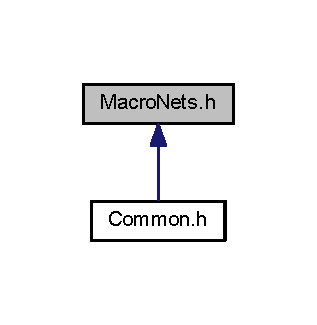
\includegraphics[width=152pt]{a00066}
\end{center}
\end{figure}
\subsection*{Data Structures}
\begin{DoxyCompactItemize}
\item 
struct \hyperlink{a00005}{ext\-Device\-Settings}
\item 
struct \hyperlink{a00007}{load\-Stage\-Nets}
\item 
struct \hyperlink{a00008}{load\-Stage\-Settings}
\item 
struct \hyperlink{a00009}{xfmr\-Stage\-Nets}
\item 
struct \hyperlink{a00010}{xfmr\-Stage\-Settings}
\item 
struct \hyperlink{a00003}{ac\-Stage\-Nets}
\item 
struct \hyperlink{a00004}{ac\-Stage\-Settings}
\end{DoxyCompactItemize}
\subsection*{Macros}
\begin{DoxyCompactItemize}
\item 
\#define \hyperlink{a00027_a007a209cd2e2b935be1f69218652edc1}{L\-O\-A\-D\-\_\-0}~0
\item 
\#define \hyperlink{a00027_a363f09c63f2ecb9086b47d72a3f3f57d}{L\-O\-A\-D\-\_\-1}~1
\item 
\#define \hyperlink{a00027_af7c1e96216e7b48160e5a03afe8ac807}{L\-O\-A\-D\-\_\-2}~2
\item 
\#define \hyperlink{a00027_a2c862ec4115c4a016b61800609f236a7}{L\-O\-A\-D\-\_\-3}~3
\item 
\#define \hyperlink{a00027_a873d529c32530ec23fbf76318011aeee}{X\-F\-M\-R\-\_\-\-S\-T\-A\-G\-E}~4
\item 
\#define \hyperlink{a00027_a3fc4318ae73eae35339f616047300b0f}{A\-C\-\_\-\-S\-T\-A\-G\-E}~5
\item 
\#define \hyperlink{a00027_ae72b26dfe821ff1cfeb352b6b54e5cbb}{E\-X\-T\-\_\-1}~6
\item 
\#define \hyperlink{a00027_a461d83d7d883765da6f6b257a7a4c385}{E\-X\-T\-\_\-2}~7
\end{DoxyCompactItemize}
\subsection*{Typedefs}
\begin{DoxyCompactItemize}
\item 
typedef enum \hyperlink{a00027_a258413561252a6c94af200747272a9f3}{ext\-Select} \hyperlink{a00027_a70b24a6c60fcd622c699e09219a34da0}{ext\-Select}
\item 
typedef struct \hyperlink{a00005}{ext\-Device\-Settings} \hyperlink{a00027_aa0c9d277e59731716a1973e29ea96246}{ext\-Device\-Settings}
\item 
typedef enum \hyperlink{a00027_a2820f1e18d921d2f1e97d53404b9fbae}{load\-Stage} \hyperlink{a00027_af7950a62c78fd817e8115e55c0f4bb44}{load\-Stage}
\item 
typedef struct \hyperlink{a00007}{load\-Stage\-Nets} \hyperlink{a00027_aae981f2f918bbbfae4517a68d60ffb45}{load\-Stage\-Nets}
\item 
typedef struct \hyperlink{a00008}{load\-Stage\-Settings} \hyperlink{a00027_a23ea7275d3010efb32f35ffe237401ff}{load\-Stage\-Settings}
\item 
typedef struct \hyperlink{a00009}{xfmr\-Stage\-Nets} \hyperlink{a00027_a583225b973f6b7cb16edbff4d3dadeab}{xfmr\-Stage\-Nets}
\item 
typedef struct \hyperlink{a00010}{xfmr\-Stage\-Settings} \hyperlink{a00027_ab13cb1eb6c11d220d249e98a5250235a}{xfmr\-Stage\-Settings}
\item 
typedef struct \hyperlink{a00003}{ac\-Stage\-Nets} \hyperlink{a00027_a8e395a646881dbb659b7fdaff0f80be0}{ac\-Stage\-Nets}
\item 
typedef struct \hyperlink{a00004}{ac\-Stage\-Settings} \hyperlink{a00027_a32c7a835db0120b8a119548c2a0337d5}{ac\-Stage\-Settings}
\end{DoxyCompactItemize}
\subsection*{Enumerations}
\begin{DoxyCompactItemize}
\item 
enum \hyperlink{a00027_a258413561252a6c94af200747272a9f3}{ext\-Select} \{ \hyperlink{a00027_a258413561252a6c94af200747272a9f3a6b8e8e9bb4b53b3fc029110541623a3c}{ext1} = 0, 
\hyperlink{a00027_a258413561252a6c94af200747272a9f3a6b3e8213ce7722257795b7a3ffb915fc}{ext2} = 1
 \}
\item 
enum \hyperlink{a00027_a2820f1e18d921d2f1e97d53404b9fbae}{load\-Stage} \{ \hyperlink{a00027_a2820f1e18d921d2f1e97d53404b9fbaeae319629172a300013df8b0149c386f96}{load1} = 0, 
\hyperlink{a00027_a2820f1e18d921d2f1e97d53404b9fbaea690fc43c88b8671aff6aed61a8a2f9c6}{load2} = 1, 
\hyperlink{a00027_a2820f1e18d921d2f1e97d53404b9fbaea861124cff343ddc4d2cc20dfe3ee7fa2}{load3} = 2, 
\hyperlink{a00027_a2820f1e18d921d2f1e97d53404b9fbaea94258908ecc1dedac8f08e7baf1156fc}{load4} = 3
 \}
\end{DoxyCompactItemize}
\subsection*{Functions}
\begin{DoxyCompactItemize}
\item 
void \hyperlink{a00027_a0ae5a77eff5aae0f7aead915fe68328b}{setup\-Nets} (slave\-Mode mode)
\item 
void \hyperlink{a00027_a776854c00eb8a571abbfb27130ba4849}{stop\-All} (void)
\item 
void \hyperlink{a00027_a24dce601551d1d81b127711d2f4aabdd}{run\-All} (void)
\end{DoxyCompactItemize}
\subsection*{Variables}
\begin{DoxyCompactItemize}
\item 
Uint16 \hyperlink{a00027_af6530cd8f296ed6bf84f4ce75ea4c9ad}{stop\-All\-Flag}
\item 
Uint16 \hyperlink{a00027_a65fcb0c0a483e3bc3433b17227fa29ac}{enable\-All\-Flag}
\item 
\hyperlink{a00005}{ext\-Device\-Settings} \hyperlink{a00027_ab8092749f4706406bb47ec950573ebed}{ext\-Settings}
\item 
\hyperlink{a00007}{load\-Stage\-Nets} \hyperlink{a00027_a0a6ae344146684f87fe8ca400640dced}{load\-Nets} \mbox{[}number\-Of\-Loads\mbox{]}
\item 
\hyperlink{a00008}{load\-Stage\-Settings} \hyperlink{a00027_acb0d5fe43ffb1c0edbb3d22409a8f346}{load\-Settings} \mbox{[}number\-Of\-Loads\mbox{]}
\item 
\hyperlink{a00009}{xfmr\-Stage\-Nets} \hyperlink{a00027_aec1d3b8f844d1d31ce7e703e50209432}{xfmr\-Nets}
\item 
\hyperlink{a00010}{xfmr\-Stage\-Settings} \hyperlink{a00027_ab8977a3c81ebfcd1b5dbe7fb49e9f832}{xfmr\-Settings}
\item 
\hyperlink{a00003}{ac\-Stage\-Nets} \hyperlink{a00027_ab73a0aedbde1954d7bf8091e07e4675c}{ac\-Nets}
\item 
\hyperlink{a00004}{ac\-Stage\-Settings} \hyperlink{a00027_aee11a0ac36813aa41597f992e943cd17}{ac\-Settings}
\end{DoxyCompactItemize}


\subsection{Detailed Description}
D\-P\-Lib macro net and value control functions. 

\subsection{Macro Definition Documentation}
\hypertarget{a00027_a3fc4318ae73eae35339f616047300b0f}{\index{Macro\-Nets.\-h@{Macro\-Nets.\-h}!A\-C\-\_\-\-S\-T\-A\-G\-E@{A\-C\-\_\-\-S\-T\-A\-G\-E}}
\index{A\-C\-\_\-\-S\-T\-A\-G\-E@{A\-C\-\_\-\-S\-T\-A\-G\-E}!MacroNets.h@{Macro\-Nets.\-h}}
\subsubsection[{A\-C\-\_\-\-S\-T\-A\-G\-E}]{\setlength{\rightskip}{0pt plus 5cm}\#define A\-C\-\_\-\-S\-T\-A\-G\-E~5}}\label{a00027_a3fc4318ae73eae35339f616047300b0f}
The index position for A\-C stage settings. \hypertarget{a00027_ae72b26dfe821ff1cfeb352b6b54e5cbb}{\index{Macro\-Nets.\-h@{Macro\-Nets.\-h}!E\-X\-T\-\_\-1@{E\-X\-T\-\_\-1}}
\index{E\-X\-T\-\_\-1@{E\-X\-T\-\_\-1}!MacroNets.h@{Macro\-Nets.\-h}}
\subsubsection[{E\-X\-T\-\_\-1}]{\setlength{\rightskip}{0pt plus 5cm}\#define E\-X\-T\-\_\-1~6}}\label{a00027_ae72b26dfe821ff1cfeb352b6b54e5cbb}
External temperature 1 channel reference. \hypertarget{a00027_a461d83d7d883765da6f6b257a7a4c385}{\index{Macro\-Nets.\-h@{Macro\-Nets.\-h}!E\-X\-T\-\_\-2@{E\-X\-T\-\_\-2}}
\index{E\-X\-T\-\_\-2@{E\-X\-T\-\_\-2}!MacroNets.h@{Macro\-Nets.\-h}}
\subsubsection[{E\-X\-T\-\_\-2}]{\setlength{\rightskip}{0pt plus 5cm}\#define E\-X\-T\-\_\-2~7}}\label{a00027_a461d83d7d883765da6f6b257a7a4c385}
External temperature 2 channel reference. \hypertarget{a00027_a007a209cd2e2b935be1f69218652edc1}{\index{Macro\-Nets.\-h@{Macro\-Nets.\-h}!L\-O\-A\-D\-\_\-0@{L\-O\-A\-D\-\_\-0}}
\index{L\-O\-A\-D\-\_\-0@{L\-O\-A\-D\-\_\-0}!MacroNets.h@{Macro\-Nets.\-h}}
\subsubsection[{L\-O\-A\-D\-\_\-0}]{\setlength{\rightskip}{0pt plus 5cm}\#define L\-O\-A\-D\-\_\-0~0}}\label{a00027_a007a209cd2e2b935be1f69218652edc1}
The index position for Load 0 settings. \hypertarget{a00027_a363f09c63f2ecb9086b47d72a3f3f57d}{\index{Macro\-Nets.\-h@{Macro\-Nets.\-h}!L\-O\-A\-D\-\_\-1@{L\-O\-A\-D\-\_\-1}}
\index{L\-O\-A\-D\-\_\-1@{L\-O\-A\-D\-\_\-1}!MacroNets.h@{Macro\-Nets.\-h}}
\subsubsection[{L\-O\-A\-D\-\_\-1}]{\setlength{\rightskip}{0pt plus 5cm}\#define L\-O\-A\-D\-\_\-1~1}}\label{a00027_a363f09c63f2ecb9086b47d72a3f3f57d}
The index position for Load 1 settings. \hypertarget{a00027_af7c1e96216e7b48160e5a03afe8ac807}{\index{Macro\-Nets.\-h@{Macro\-Nets.\-h}!L\-O\-A\-D\-\_\-2@{L\-O\-A\-D\-\_\-2}}
\index{L\-O\-A\-D\-\_\-2@{L\-O\-A\-D\-\_\-2}!MacroNets.h@{Macro\-Nets.\-h}}
\subsubsection[{L\-O\-A\-D\-\_\-2}]{\setlength{\rightskip}{0pt plus 5cm}\#define L\-O\-A\-D\-\_\-2~2}}\label{a00027_af7c1e96216e7b48160e5a03afe8ac807}
The index position for Load 2 settings. \hypertarget{a00027_a2c862ec4115c4a016b61800609f236a7}{\index{Macro\-Nets.\-h@{Macro\-Nets.\-h}!L\-O\-A\-D\-\_\-3@{L\-O\-A\-D\-\_\-3}}
\index{L\-O\-A\-D\-\_\-3@{L\-O\-A\-D\-\_\-3}!MacroNets.h@{Macro\-Nets.\-h}}
\subsubsection[{L\-O\-A\-D\-\_\-3}]{\setlength{\rightskip}{0pt plus 5cm}\#define L\-O\-A\-D\-\_\-3~3}}\label{a00027_a2c862ec4115c4a016b61800609f236a7}
The index position for Load 3 settings. \hypertarget{a00027_a873d529c32530ec23fbf76318011aeee}{\index{Macro\-Nets.\-h@{Macro\-Nets.\-h}!X\-F\-M\-R\-\_\-\-S\-T\-A\-G\-E@{X\-F\-M\-R\-\_\-\-S\-T\-A\-G\-E}}
\index{X\-F\-M\-R\-\_\-\-S\-T\-A\-G\-E@{X\-F\-M\-R\-\_\-\-S\-T\-A\-G\-E}!MacroNets.h@{Macro\-Nets.\-h}}
\subsubsection[{X\-F\-M\-R\-\_\-\-S\-T\-A\-G\-E}]{\setlength{\rightskip}{0pt plus 5cm}\#define X\-F\-M\-R\-\_\-\-S\-T\-A\-G\-E~4}}\label{a00027_a873d529c32530ec23fbf76318011aeee}
The index position for transformer stage settings. 

\subsection{Typedef Documentation}
\hypertarget{a00027_a8e395a646881dbb659b7fdaff0f80be0}{\index{Macro\-Nets.\-h@{Macro\-Nets.\-h}!ac\-Stage\-Nets@{ac\-Stage\-Nets}}
\index{ac\-Stage\-Nets@{ac\-Stage\-Nets}!MacroNets.h@{Macro\-Nets.\-h}}
\subsubsection[{ac\-Stage\-Nets}]{\setlength{\rightskip}{0pt plus 5cm}typedef struct {\bf ac\-Stage\-Nets} {\bf ac\-Stage\-Nets}}}\label{a00027_a8e395a646881dbb659b7fdaff0f80be0}
A type to allow use of the A\-C stage nets structure. \hypertarget{a00027_a32c7a835db0120b8a119548c2a0337d5}{\index{Macro\-Nets.\-h@{Macro\-Nets.\-h}!ac\-Stage\-Settings@{ac\-Stage\-Settings}}
\index{ac\-Stage\-Settings@{ac\-Stage\-Settings}!MacroNets.h@{Macro\-Nets.\-h}}
\subsubsection[{ac\-Stage\-Settings}]{\setlength{\rightskip}{0pt plus 5cm}typedef struct {\bf ac\-Stage\-Settings} {\bf ac\-Stage\-Settings}}}\label{a00027_a32c7a835db0120b8a119548c2a0337d5}
A type to allow use of the A\-C stage settings structure. \hypertarget{a00027_aa0c9d277e59731716a1973e29ea96246}{\index{Macro\-Nets.\-h@{Macro\-Nets.\-h}!ext\-Device\-Settings@{ext\-Device\-Settings}}
\index{ext\-Device\-Settings@{ext\-Device\-Settings}!MacroNets.h@{Macro\-Nets.\-h}}
\subsubsection[{ext\-Device\-Settings}]{\setlength{\rightskip}{0pt plus 5cm}typedef struct {\bf ext\-Device\-Settings} {\bf ext\-Device\-Settings}}}\label{a00027_aa0c9d277e59731716a1973e29ea96246}
A type to allow use of the external device settings structure. \hypertarget{a00027_a70b24a6c60fcd622c699e09219a34da0}{\index{Macro\-Nets.\-h@{Macro\-Nets.\-h}!ext\-Select@{ext\-Select}}
\index{ext\-Select@{ext\-Select}!MacroNets.h@{Macro\-Nets.\-h}}
\subsubsection[{ext\-Select}]{\setlength{\rightskip}{0pt plus 5cm}typedef enum {\bf ext\-Select} {\bf ext\-Select}}}\label{a00027_a70b24a6c60fcd622c699e09219a34da0}
A type that allow specification of an external sensor. \hypertarget{a00027_af7950a62c78fd817e8115e55c0f4bb44}{\index{Macro\-Nets.\-h@{Macro\-Nets.\-h}!load\-Stage@{load\-Stage}}
\index{load\-Stage@{load\-Stage}!MacroNets.h@{Macro\-Nets.\-h}}
\subsubsection[{load\-Stage}]{\setlength{\rightskip}{0pt plus 5cm}typedef enum {\bf load\-Stage} {\bf load\-Stage}}}\label{a00027_af7950a62c78fd817e8115e55c0f4bb44}
A type that allow specification of a load. \hypertarget{a00027_aae981f2f918bbbfae4517a68d60ffb45}{\index{Macro\-Nets.\-h@{Macro\-Nets.\-h}!load\-Stage\-Nets@{load\-Stage\-Nets}}
\index{load\-Stage\-Nets@{load\-Stage\-Nets}!MacroNets.h@{Macro\-Nets.\-h}}
\subsubsection[{load\-Stage\-Nets}]{\setlength{\rightskip}{0pt plus 5cm}typedef struct {\bf load\-Stage\-Nets} {\bf load\-Stage\-Nets}}}\label{a00027_aae981f2f918bbbfae4517a68d60ffb45}
A type to allow use of the load stage nets structure. \hypertarget{a00027_a23ea7275d3010efb32f35ffe237401ff}{\index{Macro\-Nets.\-h@{Macro\-Nets.\-h}!load\-Stage\-Settings@{load\-Stage\-Settings}}
\index{load\-Stage\-Settings@{load\-Stage\-Settings}!MacroNets.h@{Macro\-Nets.\-h}}
\subsubsection[{load\-Stage\-Settings}]{\setlength{\rightskip}{0pt plus 5cm}typedef struct {\bf load\-Stage\-Settings} {\bf load\-Stage\-Settings}}}\label{a00027_a23ea7275d3010efb32f35ffe237401ff}
A type to allow use of the load stage settings structure. \hypertarget{a00027_a583225b973f6b7cb16edbff4d3dadeab}{\index{Macro\-Nets.\-h@{Macro\-Nets.\-h}!xfmr\-Stage\-Nets@{xfmr\-Stage\-Nets}}
\index{xfmr\-Stage\-Nets@{xfmr\-Stage\-Nets}!MacroNets.h@{Macro\-Nets.\-h}}
\subsubsection[{xfmr\-Stage\-Nets}]{\setlength{\rightskip}{0pt plus 5cm}typedef struct {\bf xfmr\-Stage\-Nets} {\bf xfmr\-Stage\-Nets}}}\label{a00027_a583225b973f6b7cb16edbff4d3dadeab}
A type to allow use of the transformer stage nets structure. \hypertarget{a00027_ab13cb1eb6c11d220d249e98a5250235a}{\index{Macro\-Nets.\-h@{Macro\-Nets.\-h}!xfmr\-Stage\-Settings@{xfmr\-Stage\-Settings}}
\index{xfmr\-Stage\-Settings@{xfmr\-Stage\-Settings}!MacroNets.h@{Macro\-Nets.\-h}}
\subsubsection[{xfmr\-Stage\-Settings}]{\setlength{\rightskip}{0pt plus 5cm}typedef struct {\bf xfmr\-Stage\-Settings} {\bf xfmr\-Stage\-Settings}}}\label{a00027_ab13cb1eb6c11d220d249e98a5250235a}
A type to allow use of the A\-C stage settings structure. 

\subsection{Enumeration Type Documentation}
\hypertarget{a00027_a258413561252a6c94af200747272a9f3}{\index{Macro\-Nets.\-h@{Macro\-Nets.\-h}!ext\-Select@{ext\-Select}}
\index{ext\-Select@{ext\-Select}!MacroNets.h@{Macro\-Nets.\-h}}
\subsubsection[{ext\-Select}]{\setlength{\rightskip}{0pt plus 5cm}enum {\bf ext\-Select}}}\label{a00027_a258413561252a6c94af200747272a9f3}
The possible external sensor selections. \begin{Desc}
\item[Enumerator]\par
\begin{description}
\index{ext1@{ext1}!Macro\-Nets.\-h@{Macro\-Nets.\-h}}\index{Macro\-Nets.\-h@{Macro\-Nets.\-h}!ext1@{ext1}}\item[{\em 
\hypertarget{a00027_a258413561252a6c94af200747272a9f3a6b8e8e9bb4b53b3fc029110541623a3c}{ext1}\label{a00027_a258413561252a6c94af200747272a9f3a6b8e8e9bb4b53b3fc029110541623a3c}
}]External sensor 1. \index{ext2@{ext2}!Macro\-Nets.\-h@{Macro\-Nets.\-h}}\index{Macro\-Nets.\-h@{Macro\-Nets.\-h}!ext2@{ext2}}\item[{\em 
\hypertarget{a00027_a258413561252a6c94af200747272a9f3a6b3e8213ce7722257795b7a3ffb915fc}{ext2}\label{a00027_a258413561252a6c94af200747272a9f3a6b3e8213ce7722257795b7a3ffb915fc}
}]External sensor 2. \end{description}
\end{Desc}
\hypertarget{a00027_a2820f1e18d921d2f1e97d53404b9fbae}{\index{Macro\-Nets.\-h@{Macro\-Nets.\-h}!load\-Stage@{load\-Stage}}
\index{load\-Stage@{load\-Stage}!MacroNets.h@{Macro\-Nets.\-h}}
\subsubsection[{load\-Stage}]{\setlength{\rightskip}{0pt plus 5cm}enum {\bf load\-Stage}}}\label{a00027_a2820f1e18d921d2f1e97d53404b9fbae}
The possible load stage selections. \begin{Desc}
\item[Enumerator]\par
\begin{description}
\index{load1@{load1}!Macro\-Nets.\-h@{Macro\-Nets.\-h}}\index{Macro\-Nets.\-h@{Macro\-Nets.\-h}!load1@{load1}}\item[{\em 
\hypertarget{a00027_a2820f1e18d921d2f1e97d53404b9fbaeae319629172a300013df8b0149c386f96}{load1}\label{a00027_a2820f1e18d921d2f1e97d53404b9fbaeae319629172a300013df8b0149c386f96}
}]Load 1. \index{load2@{load2}!Macro\-Nets.\-h@{Macro\-Nets.\-h}}\index{Macro\-Nets.\-h@{Macro\-Nets.\-h}!load2@{load2}}\item[{\em 
\hypertarget{a00027_a2820f1e18d921d2f1e97d53404b9fbaea690fc43c88b8671aff6aed61a8a2f9c6}{load2}\label{a00027_a2820f1e18d921d2f1e97d53404b9fbaea690fc43c88b8671aff6aed61a8a2f9c6}
}]Load 2. \index{load3@{load3}!Macro\-Nets.\-h@{Macro\-Nets.\-h}}\index{Macro\-Nets.\-h@{Macro\-Nets.\-h}!load3@{load3}}\item[{\em 
\hypertarget{a00027_a2820f1e18d921d2f1e97d53404b9fbaea861124cff343ddc4d2cc20dfe3ee7fa2}{load3}\label{a00027_a2820f1e18d921d2f1e97d53404b9fbaea861124cff343ddc4d2cc20dfe3ee7fa2}
}]Load 3. \index{load4@{load4}!Macro\-Nets.\-h@{Macro\-Nets.\-h}}\index{Macro\-Nets.\-h@{Macro\-Nets.\-h}!load4@{load4}}\item[{\em 
\hypertarget{a00027_a2820f1e18d921d2f1e97d53404b9fbaea94258908ecc1dedac8f08e7baf1156fc}{load4}\label{a00027_a2820f1e18d921d2f1e97d53404b9fbaea94258908ecc1dedac8f08e7baf1156fc}
}]Load 4. \end{description}
\end{Desc}


\subsection{Function Documentation}
\hypertarget{a00027_a24dce601551d1d81b127711d2f4aabdd}{\index{Macro\-Nets.\-h@{Macro\-Nets.\-h}!run\-All@{run\-All}}
\index{run\-All@{run\-All}!MacroNets.h@{Macro\-Nets.\-h}}
\subsubsection[{run\-All}]{\setlength{\rightskip}{0pt plus 5cm}void run\-All (
\begin{DoxyParamCaption}
\item[{void}]{}
\end{DoxyParamCaption}
)}}\label{a00027_a24dce601551d1d81b127711d2f4aabdd}
Enables all I\-I\-R filter control law reference inputs. \hypertarget{a00027_a0ae5a77eff5aae0f7aead915fe68328b}{\index{Macro\-Nets.\-h@{Macro\-Nets.\-h}!setup\-Nets@{setup\-Nets}}
\index{setup\-Nets@{setup\-Nets}!MacroNets.h@{Macro\-Nets.\-h}}
\subsubsection[{setup\-Nets}]{\setlength{\rightskip}{0pt plus 5cm}void setup\-Nets (
\begin{DoxyParamCaption}
\item[{slave\-Mode}]{mode}
\end{DoxyParamCaption}
)}}\label{a00027_a0ae5a77eff5aae0f7aead915fe68328b}
Initialises macro settings and nets. I\-I\-R control law coefficients are handled outside of this function. \begin{DoxyWarning}{Warning}
This M\-U\-S\-T be called after D\-P\-L\-\_\-\-I\-N\-I\-T() 

This M\-U\-S\-T be called after pwm\-Macro\-Config() 
\end{DoxyWarning}

\begin{DoxyParams}[1]{Parameters}
\mbox{\tt in}  & {\em mode} & Selects the test unit mode to allow correct macro net connection. \\
\hline
\end{DoxyParams}
\hypertarget{a00027_a776854c00eb8a571abbfb27130ba4849}{\index{Macro\-Nets.\-h@{Macro\-Nets.\-h}!stop\-All@{stop\-All}}
\index{stop\-All@{stop\-All}!MacroNets.h@{Macro\-Nets.\-h}}
\subsubsection[{stop\-All}]{\setlength{\rightskip}{0pt plus 5cm}void stop\-All (
\begin{DoxyParamCaption}
\item[{void}]{}
\end{DoxyParamCaption}
)}}\label{a00027_a776854c00eb8a571abbfb27130ba4849}
Disables all circuit sections, zeroes all I\-I\-R references and flags each stage as disabled. 

\subsection{Variable Documentation}
\hypertarget{a00027_ab73a0aedbde1954d7bf8091e07e4675c}{\index{Macro\-Nets.\-h@{Macro\-Nets.\-h}!ac\-Nets@{ac\-Nets}}
\index{ac\-Nets@{ac\-Nets}!MacroNets.h@{Macro\-Nets.\-h}}
\subsubsection[{ac\-Nets}]{\setlength{\rightskip}{0pt plus 5cm}{\bf ac\-Stage\-Nets} ac\-Nets}}\label{a00027_ab73a0aedbde1954d7bf8091e07e4675c}
A global instance of the A\-C nets structure. \hypertarget{a00027_aee11a0ac36813aa41597f992e943cd17}{\index{Macro\-Nets.\-h@{Macro\-Nets.\-h}!ac\-Settings@{ac\-Settings}}
\index{ac\-Settings@{ac\-Settings}!MacroNets.h@{Macro\-Nets.\-h}}
\subsubsection[{ac\-Settings}]{\setlength{\rightskip}{0pt plus 5cm}{\bf ac\-Stage\-Settings} ac\-Settings}}\label{a00027_aee11a0ac36813aa41597f992e943cd17}
A global instance of the A\-C settings structure. \hypertarget{a00027_a65fcb0c0a483e3bc3433b17227fa29ac}{\index{Macro\-Nets.\-h@{Macro\-Nets.\-h}!enable\-All\-Flag@{enable\-All\-Flag}}
\index{enable\-All\-Flag@{enable\-All\-Flag}!MacroNets.h@{Macro\-Nets.\-h}}
\subsubsection[{enable\-All\-Flag}]{\setlength{\rightskip}{0pt plus 5cm}Uint16 enable\-All\-Flag}}\label{a00027_a65fcb0c0a483e3bc3433b17227fa29ac}
Enable-\/all condition flag that allows status communication between the state machine tasks. \hypertarget{a00027_ab8092749f4706406bb47ec950573ebed}{\index{Macro\-Nets.\-h@{Macro\-Nets.\-h}!ext\-Settings@{ext\-Settings}}
\index{ext\-Settings@{ext\-Settings}!MacroNets.h@{Macro\-Nets.\-h}}
\subsubsection[{ext\-Settings}]{\setlength{\rightskip}{0pt plus 5cm}{\bf ext\-Device\-Settings} ext\-Settings}}\label{a00027_ab8092749f4706406bb47ec950573ebed}
A global instance of the external device settings structure. \hypertarget{a00027_a0a6ae344146684f87fe8ca400640dced}{\index{Macro\-Nets.\-h@{Macro\-Nets.\-h}!load\-Nets@{load\-Nets}}
\index{load\-Nets@{load\-Nets}!MacroNets.h@{Macro\-Nets.\-h}}
\subsubsection[{load\-Nets}]{\setlength{\rightskip}{0pt plus 5cm}{\bf load\-Stage\-Nets} load\-Nets\mbox{[}number\-Of\-Loads\mbox{]}}}\label{a00027_a0a6ae344146684f87fe8ca400640dced}
A global array instance of the load nets structure that collects the nets for all 4 loads. \hypertarget{a00027_acb0d5fe43ffb1c0edbb3d22409a8f346}{\index{Macro\-Nets.\-h@{Macro\-Nets.\-h}!load\-Settings@{load\-Settings}}
\index{load\-Settings@{load\-Settings}!MacroNets.h@{Macro\-Nets.\-h}}
\subsubsection[{load\-Settings}]{\setlength{\rightskip}{0pt plus 5cm}{\bf load\-Stage\-Settings} load\-Settings\mbox{[}number\-Of\-Loads\mbox{]}}}\label{a00027_acb0d5fe43ffb1c0edbb3d22409a8f346}
A global array instance of the load settings structure that collects the settings for all 4 loads. \hypertarget{a00027_af6530cd8f296ed6bf84f4ce75ea4c9ad}{\index{Macro\-Nets.\-h@{Macro\-Nets.\-h}!stop\-All\-Flag@{stop\-All\-Flag}}
\index{stop\-All\-Flag@{stop\-All\-Flag}!MacroNets.h@{Macro\-Nets.\-h}}
\subsubsection[{stop\-All\-Flag}]{\setlength{\rightskip}{0pt plus 5cm}Uint16 stop\-All\-Flag}}\label{a00027_af6530cd8f296ed6bf84f4ce75ea4c9ad}
Stop-\/all condition flag that allows status communication between the state machine tasks. \hypertarget{a00027_aec1d3b8f844d1d31ce7e703e50209432}{\index{Macro\-Nets.\-h@{Macro\-Nets.\-h}!xfmr\-Nets@{xfmr\-Nets}}
\index{xfmr\-Nets@{xfmr\-Nets}!MacroNets.h@{Macro\-Nets.\-h}}
\subsubsection[{xfmr\-Nets}]{\setlength{\rightskip}{0pt plus 5cm}{\bf xfmr\-Stage\-Nets} xfmr\-Nets}}\label{a00027_aec1d3b8f844d1d31ce7e703e50209432}
A global instance of the transformer nets structure. \hypertarget{a00027_ab8977a3c81ebfcd1b5dbe7fb49e9f832}{\index{Macro\-Nets.\-h@{Macro\-Nets.\-h}!xfmr\-Settings@{xfmr\-Settings}}
\index{xfmr\-Settings@{xfmr\-Settings}!MacroNets.h@{Macro\-Nets.\-h}}
\subsubsection[{xfmr\-Settings}]{\setlength{\rightskip}{0pt plus 5cm}{\bf xfmr\-Stage\-Settings} xfmr\-Settings}}\label{a00027_ab8977a3c81ebfcd1b5dbe7fb49e9f832}
A global instance of the transformer settings structure. 
\hypertarget{a00030}{\section{Ocp.\-h File Reference}
\label{a00030}\index{Ocp.\-h@{Ocp.\-h}}
}


Over-\/current protection functions.  


This graph shows which files directly or indirectly include this file\-:\nopagebreak
\begin{figure}[H]
\begin{center}
\leavevmode
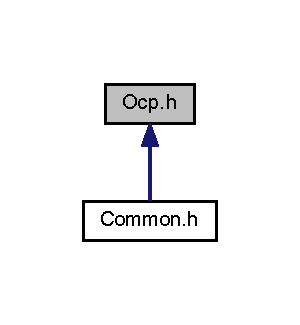
\includegraphics[width=144pt]{a00067}
\end{center}
\end{figure}
\subsection*{Macros}
\begin{DoxyCompactItemize}
\item 
\#define \hyperlink{a00030_a4ec4aa0e60bea1a3e34167b2571a65de}{L\-O\-A\-D1\-\_\-\-O\-C\-P\-\_\-\-T\-R\-I\-P}~1
\item 
\#define \hyperlink{a00030_af45ed9a707fb208c436f4f9cfd0adfec}{L\-O\-A\-D2\-\_\-\-O\-C\-P\-\_\-\-T\-R\-I\-P}~2
\item 
\#define \hyperlink{a00030_a94b1ce836bab1ddbaf5a153cf84f42b7}{L\-O\-A\-D3\-\_\-\-O\-C\-P\-\_\-\-T\-R\-I\-P}~4
\item 
\#define \hyperlink{a00030_a271333484c12cc2d424b2870bbd2ea77}{L\-O\-A\-D4\-\_\-\-O\-C\-P\-\_\-\-T\-R\-I\-P}~8
\item 
\#define \hyperlink{a00030_ad4ef44d1890a81d34d453203c204384a}{D\-C\-M\-I\-D\-\_\-\-O\-C\-P\-\_\-\-T\-R\-I\-P}~16
\item 
\#define \hyperlink{a00030_a79277b6c4861afbef292e26f4360b224}{D\-C\-H\-V\-\_\-\-O\-C\-P\-\_\-\-T\-R\-I\-P}~32
\item 
\#define \hyperlink{a00030_a53e3b040fd854d92e865a4e59f1630a2}{A\-C\-\_\-\-O\-C\-P\-\_\-\-T\-R\-I\-P}~64
\end{DoxyCompactItemize}
\subsection*{Functions}
\begin{DoxyCompactItemize}
\item 
Uint16 \hyperlink{a00030_a5da4bbec3c1f5d83678a06f574cf664a}{set\-Load\-Ocp\-Level} (\hyperlink{a00027_a2820f1e18d921d2f1e97d53404b9fbae}{load\-Stage} load, float32 dc\-Level)
\item 
Uint16 \hyperlink{a00030_a3c056a05cc718b13f07af5e2421b2813}{get\-Load\-Ocp\-Level} (\hyperlink{a00027_a2820f1e18d921d2f1e97d53404b9fbae}{load\-Stage} load, float32 $\ast$dc\-Level)
\item 
Uint16 \hyperlink{a00030_a59c9eb4cd335a46e4c33651a26ecbf10}{check\-Load\-Ocp} (\hyperlink{a00027_a2820f1e18d921d2f1e97d53404b9fbae}{load\-Stage} load)
\item 
Uint16 \hyperlink{a00030_a89c27fb6ed80f4487598a23987aef528}{get\-Load\-Ocp\-State} (\hyperlink{a00027_a2820f1e18d921d2f1e97d53404b9fbae}{load\-Stage} load)
\item 
Uint16 \hyperlink{a00030_a21a8a91440da87204edb7e67d3fde578}{clear\-Load\-Ocp} (\hyperlink{a00027_a2820f1e18d921d2f1e97d53404b9fbae}{load\-Stage} load)
\item 
Uint16 \hyperlink{a00030_a2688d88502221ff2a5f79091a708408e}{set\-Dc\-Mid\-Ocp\-Level} (float32 dc\-Level)
\item 
Uint16 \hyperlink{a00030_ae7d51f03d13dea383fd543b1c8f19e49}{get\-Dc\-Mid\-Ocp\-Level} (float32 $\ast$dc\-Level)
\item 
Uint16 \hyperlink{a00030_acdbe7d23734fc6f4fbc3cc7ebe8ffb51}{check\-Dc\-Mid\-Ocp} (void)
\item 
Uint16 \hyperlink{a00030_a2144c56f3ede583b197273a88bd53801}{get\-Dc\-Mid\-Ocp\-State} (void)
\item 
Uint16 \hyperlink{a00030_a8f57a6183f616d09458d9cd3dfd84766}{clear\-Dc\-Mid\-Ocp} (void)
\item 
Uint16 \hyperlink{a00030_a4433a05d2924b2a5cc659ab8e8c8ff8a}{set\-Ac\-Ocp\-Level} (float32 pk\-Level)
\item 
Uint16 \hyperlink{a00030_a7273f23cc84891cc7cda8d3081c6b946}{get\-Ac\-Ocp\-Level} (float32 $\ast$pk\-Level)
\item 
Uint16 \hyperlink{a00030_aecbc5bcbe9cc0babef4d0c742ac82170}{trip\-Ac\-Ocp} (void)
\item 
Uint16 \hyperlink{a00030_ad496df3ce8212c5a991e62c8a44ff060}{get\-Ac\-Ocp\-State} (void)
\item 
Uint16 \hyperlink{a00030_ad2757e72816f7a5c6a6a70760e9012a8}{clear\-Ac\-Ocp} (void)
\end{DoxyCompactItemize}


\subsection{Detailed Description}
Over-\/current protection functions. These functions require that the relevant relevant measurement scales be set before use. 

\subsection{Macro Definition Documentation}
\hypertarget{a00030_a53e3b040fd854d92e865a4e59f1630a2}{\index{Ocp.\-h@{Ocp.\-h}!A\-C\-\_\-\-O\-C\-P\-\_\-\-T\-R\-I\-P@{A\-C\-\_\-\-O\-C\-P\-\_\-\-T\-R\-I\-P}}
\index{A\-C\-\_\-\-O\-C\-P\-\_\-\-T\-R\-I\-P@{A\-C\-\_\-\-O\-C\-P\-\_\-\-T\-R\-I\-P}!Ocp.h@{Ocp.\-h}}
\subsubsection[{A\-C\-\_\-\-O\-C\-P\-\_\-\-T\-R\-I\-P}]{\setlength{\rightskip}{0pt plus 5cm}\#define A\-C\-\_\-\-O\-C\-P\-\_\-\-T\-R\-I\-P~64}}\label{a00030_a53e3b040fd854d92e865a4e59f1630a2}
O\-C\-P flag register A\-C bit. \hypertarget{a00030_a79277b6c4861afbef292e26f4360b224}{\index{Ocp.\-h@{Ocp.\-h}!D\-C\-H\-V\-\_\-\-O\-C\-P\-\_\-\-T\-R\-I\-P@{D\-C\-H\-V\-\_\-\-O\-C\-P\-\_\-\-T\-R\-I\-P}}
\index{D\-C\-H\-V\-\_\-\-O\-C\-P\-\_\-\-T\-R\-I\-P@{D\-C\-H\-V\-\_\-\-O\-C\-P\-\_\-\-T\-R\-I\-P}!Ocp.h@{Ocp.\-h}}
\subsubsection[{D\-C\-H\-V\-\_\-\-O\-C\-P\-\_\-\-T\-R\-I\-P}]{\setlength{\rightskip}{0pt plus 5cm}\#define D\-C\-H\-V\-\_\-\-O\-C\-P\-\_\-\-T\-R\-I\-P~32}}\label{a00030_a79277b6c4861afbef292e26f4360b224}
O\-C\-P flag register D\-C H\-V bit. \hypertarget{a00030_ad4ef44d1890a81d34d453203c204384a}{\index{Ocp.\-h@{Ocp.\-h}!D\-C\-M\-I\-D\-\_\-\-O\-C\-P\-\_\-\-T\-R\-I\-P@{D\-C\-M\-I\-D\-\_\-\-O\-C\-P\-\_\-\-T\-R\-I\-P}}
\index{D\-C\-M\-I\-D\-\_\-\-O\-C\-P\-\_\-\-T\-R\-I\-P@{D\-C\-M\-I\-D\-\_\-\-O\-C\-P\-\_\-\-T\-R\-I\-P}!Ocp.h@{Ocp.\-h}}
\subsubsection[{D\-C\-M\-I\-D\-\_\-\-O\-C\-P\-\_\-\-T\-R\-I\-P}]{\setlength{\rightskip}{0pt plus 5cm}\#define D\-C\-M\-I\-D\-\_\-\-O\-C\-P\-\_\-\-T\-R\-I\-P~16}}\label{a00030_ad4ef44d1890a81d34d453203c204384a}
O\-C\-P flag register D\-C M\-I\-D bit. \hypertarget{a00030_a4ec4aa0e60bea1a3e34167b2571a65de}{\index{Ocp.\-h@{Ocp.\-h}!L\-O\-A\-D1\-\_\-\-O\-C\-P\-\_\-\-T\-R\-I\-P@{L\-O\-A\-D1\-\_\-\-O\-C\-P\-\_\-\-T\-R\-I\-P}}
\index{L\-O\-A\-D1\-\_\-\-O\-C\-P\-\_\-\-T\-R\-I\-P@{L\-O\-A\-D1\-\_\-\-O\-C\-P\-\_\-\-T\-R\-I\-P}!Ocp.h@{Ocp.\-h}}
\subsubsection[{L\-O\-A\-D1\-\_\-\-O\-C\-P\-\_\-\-T\-R\-I\-P}]{\setlength{\rightskip}{0pt plus 5cm}\#define L\-O\-A\-D1\-\_\-\-O\-C\-P\-\_\-\-T\-R\-I\-P~1}}\label{a00030_a4ec4aa0e60bea1a3e34167b2571a65de}
O\-C\-P flag register load 1 bit. \hypertarget{a00030_af45ed9a707fb208c436f4f9cfd0adfec}{\index{Ocp.\-h@{Ocp.\-h}!L\-O\-A\-D2\-\_\-\-O\-C\-P\-\_\-\-T\-R\-I\-P@{L\-O\-A\-D2\-\_\-\-O\-C\-P\-\_\-\-T\-R\-I\-P}}
\index{L\-O\-A\-D2\-\_\-\-O\-C\-P\-\_\-\-T\-R\-I\-P@{L\-O\-A\-D2\-\_\-\-O\-C\-P\-\_\-\-T\-R\-I\-P}!Ocp.h@{Ocp.\-h}}
\subsubsection[{L\-O\-A\-D2\-\_\-\-O\-C\-P\-\_\-\-T\-R\-I\-P}]{\setlength{\rightskip}{0pt plus 5cm}\#define L\-O\-A\-D2\-\_\-\-O\-C\-P\-\_\-\-T\-R\-I\-P~2}}\label{a00030_af45ed9a707fb208c436f4f9cfd0adfec}
O\-C\-P flag register load 2 bit. \hypertarget{a00030_a94b1ce836bab1ddbaf5a153cf84f42b7}{\index{Ocp.\-h@{Ocp.\-h}!L\-O\-A\-D3\-\_\-\-O\-C\-P\-\_\-\-T\-R\-I\-P@{L\-O\-A\-D3\-\_\-\-O\-C\-P\-\_\-\-T\-R\-I\-P}}
\index{L\-O\-A\-D3\-\_\-\-O\-C\-P\-\_\-\-T\-R\-I\-P@{L\-O\-A\-D3\-\_\-\-O\-C\-P\-\_\-\-T\-R\-I\-P}!Ocp.h@{Ocp.\-h}}
\subsubsection[{L\-O\-A\-D3\-\_\-\-O\-C\-P\-\_\-\-T\-R\-I\-P}]{\setlength{\rightskip}{0pt plus 5cm}\#define L\-O\-A\-D3\-\_\-\-O\-C\-P\-\_\-\-T\-R\-I\-P~4}}\label{a00030_a94b1ce836bab1ddbaf5a153cf84f42b7}
O\-C\-P flag register load 3 bit. \hypertarget{a00030_a271333484c12cc2d424b2870bbd2ea77}{\index{Ocp.\-h@{Ocp.\-h}!L\-O\-A\-D4\-\_\-\-O\-C\-P\-\_\-\-T\-R\-I\-P@{L\-O\-A\-D4\-\_\-\-O\-C\-P\-\_\-\-T\-R\-I\-P}}
\index{L\-O\-A\-D4\-\_\-\-O\-C\-P\-\_\-\-T\-R\-I\-P@{L\-O\-A\-D4\-\_\-\-O\-C\-P\-\_\-\-T\-R\-I\-P}!Ocp.h@{Ocp.\-h}}
\subsubsection[{L\-O\-A\-D4\-\_\-\-O\-C\-P\-\_\-\-T\-R\-I\-P}]{\setlength{\rightskip}{0pt plus 5cm}\#define L\-O\-A\-D4\-\_\-\-O\-C\-P\-\_\-\-T\-R\-I\-P~8}}\label{a00030_a271333484c12cc2d424b2870bbd2ea77}
O\-C\-P flag register load 4 bit. 

\subsection{Function Documentation}
\hypertarget{a00030_acdbe7d23734fc6f4fbc3cc7ebe8ffb51}{\index{Ocp.\-h@{Ocp.\-h}!check\-Dc\-Mid\-Ocp@{check\-Dc\-Mid\-Ocp}}
\index{check\-Dc\-Mid\-Ocp@{check\-Dc\-Mid\-Ocp}!Ocp.h@{Ocp.\-h}}
\subsubsection[{check\-Dc\-Mid\-Ocp}]{\setlength{\rightskip}{0pt plus 5cm}Uint16 check\-Dc\-Mid\-Ocp (
\begin{DoxyParamCaption}
\item[{void}]{}
\end{DoxyParamCaption}
)}}\label{a00030_acdbe7d23734fc6f4fbc3cc7ebe8ffb51}
Checks the current reading of the D\-C stage against the D\-C O\-C\-P limit. Raises the D\-C O\-C\-P flag if the reading is above the limit. \begin{DoxyReturn}{Returns}
Error status 
\end{DoxyReturn}
\hypertarget{a00030_a59c9eb4cd335a46e4c33651a26ecbf10}{\index{Ocp.\-h@{Ocp.\-h}!check\-Load\-Ocp@{check\-Load\-Ocp}}
\index{check\-Load\-Ocp@{check\-Load\-Ocp}!Ocp.h@{Ocp.\-h}}
\subsubsection[{check\-Load\-Ocp}]{\setlength{\rightskip}{0pt plus 5cm}Uint16 check\-Load\-Ocp (
\begin{DoxyParamCaption}
\item[{{\bf load\-Stage}}]{load}
\end{DoxyParamCaption}
)}}\label{a00030_a59c9eb4cd335a46e4c33651a26ecbf10}
Checks the current reading of the specified load against the load O\-C\-P limit. Raises the load O\-C\-P flag if the reading is above the limit. 
\begin{DoxyParams}[1]{Parameters}
\mbox{\tt in}  & {\em load} & Specifies the load on which the reading is to be tested. \\
\hline
\end{DoxyParams}
\begin{DoxyReturn}{Returns}
Error status 
\end{DoxyReturn}
\hypertarget{a00030_ad2757e72816f7a5c6a6a70760e9012a8}{\index{Ocp.\-h@{Ocp.\-h}!clear\-Ac\-Ocp@{clear\-Ac\-Ocp}}
\index{clear\-Ac\-Ocp@{clear\-Ac\-Ocp}!Ocp.h@{Ocp.\-h}}
\subsubsection[{clear\-Ac\-Ocp}]{\setlength{\rightskip}{0pt plus 5cm}Uint16 clear\-Ac\-Ocp (
\begin{DoxyParamCaption}
\item[{void}]{}
\end{DoxyParamCaption}
)}}\label{a00030_ad2757e72816f7a5c6a6a70760e9012a8}
Clears the A\-C stage O\-C\-P state. \begin{DoxyReturn}{Returns}
Error status. 
\end{DoxyReturn}
\hypertarget{a00030_a8f57a6183f616d09458d9cd3dfd84766}{\index{Ocp.\-h@{Ocp.\-h}!clear\-Dc\-Mid\-Ocp@{clear\-Dc\-Mid\-Ocp}}
\index{clear\-Dc\-Mid\-Ocp@{clear\-Dc\-Mid\-Ocp}!Ocp.h@{Ocp.\-h}}
\subsubsection[{clear\-Dc\-Mid\-Ocp}]{\setlength{\rightskip}{0pt plus 5cm}Uint16 clear\-Dc\-Mid\-Ocp (
\begin{DoxyParamCaption}
\item[{void}]{}
\end{DoxyParamCaption}
)}}\label{a00030_a8f57a6183f616d09458d9cd3dfd84766}
Clears the D\-C stage O\-C\-P state. \begin{DoxyReturn}{Returns}
Error status. 
\end{DoxyReturn}
\hypertarget{a00030_a21a8a91440da87204edb7e67d3fde578}{\index{Ocp.\-h@{Ocp.\-h}!clear\-Load\-Ocp@{clear\-Load\-Ocp}}
\index{clear\-Load\-Ocp@{clear\-Load\-Ocp}!Ocp.h@{Ocp.\-h}}
\subsubsection[{clear\-Load\-Ocp}]{\setlength{\rightskip}{0pt plus 5cm}Uint16 clear\-Load\-Ocp (
\begin{DoxyParamCaption}
\item[{{\bf load\-Stage}}]{load}
\end{DoxyParamCaption}
)}}\label{a00030_a21a8a91440da87204edb7e67d3fde578}
Clears the O\-C\-P state for the specified load. 
\begin{DoxyParams}[1]{Parameters}
\mbox{\tt in}  & {\em load} & Specifies the load for which the O\-C\-P state is to be cleared. \\
\hline
\end{DoxyParams}
\begin{DoxyReturn}{Returns}
Error status. 
\end{DoxyReturn}
\hypertarget{a00030_a7273f23cc84891cc7cda8d3081c6b946}{\index{Ocp.\-h@{Ocp.\-h}!get\-Ac\-Ocp\-Level@{get\-Ac\-Ocp\-Level}}
\index{get\-Ac\-Ocp\-Level@{get\-Ac\-Ocp\-Level}!Ocp.h@{Ocp.\-h}}
\subsubsection[{get\-Ac\-Ocp\-Level}]{\setlength{\rightskip}{0pt plus 5cm}Uint16 get\-Ac\-Ocp\-Level (
\begin{DoxyParamCaption}
\item[{float32 $\ast$}]{pk\-Level}
\end{DoxyParamCaption}
)}}\label{a00030_a7273f23cc84891cc7cda8d3081c6b946}
Queries the over current protection level for the A\-C stage. 
\begin{DoxyParams}[1]{Parameters}
\mbox{\tt out}  & {\em pk\-Level} & Pointer to location at which to place the query result (amps). \\
\hline
\end{DoxyParams}
\begin{DoxyReturn}{Returns}
Error status. 
\end{DoxyReturn}
\hypertarget{a00030_ad496df3ce8212c5a991e62c8a44ff060}{\index{Ocp.\-h@{Ocp.\-h}!get\-Ac\-Ocp\-State@{get\-Ac\-Ocp\-State}}
\index{get\-Ac\-Ocp\-State@{get\-Ac\-Ocp\-State}!Ocp.h@{Ocp.\-h}}
\subsubsection[{get\-Ac\-Ocp\-State}]{\setlength{\rightskip}{0pt plus 5cm}Uint16 get\-Ac\-Ocp\-State (
\begin{DoxyParamCaption}
\item[{void}]{}
\end{DoxyParamCaption}
)}}\label{a00030_ad496df3ce8212c5a991e62c8a44ff060}
Queries the state of the A\-C O\-C\-P flag. \begin{DoxyReturn}{Returns}
True if O\-C\-P flag has been raised. 
\end{DoxyReturn}
\hypertarget{a00030_ae7d51f03d13dea383fd543b1c8f19e49}{\index{Ocp.\-h@{Ocp.\-h}!get\-Dc\-Mid\-Ocp\-Level@{get\-Dc\-Mid\-Ocp\-Level}}
\index{get\-Dc\-Mid\-Ocp\-Level@{get\-Dc\-Mid\-Ocp\-Level}!Ocp.h@{Ocp.\-h}}
\subsubsection[{get\-Dc\-Mid\-Ocp\-Level}]{\setlength{\rightskip}{0pt plus 5cm}Uint16 get\-Dc\-Mid\-Ocp\-Level (
\begin{DoxyParamCaption}
\item[{float32 $\ast$}]{dc\-Level}
\end{DoxyParamCaption}
)}}\label{a00030_ae7d51f03d13dea383fd543b1c8f19e49}
Queries the over current protection level for the D\-C stage. 
\begin{DoxyParams}[1]{Parameters}
\mbox{\tt out}  & {\em dc\-Level} & Pointer to location at which to place the query result (amps). \\
\hline
\end{DoxyParams}
\begin{DoxyReturn}{Returns}
Error status. 
\end{DoxyReturn}
\hypertarget{a00030_a2144c56f3ede583b197273a88bd53801}{\index{Ocp.\-h@{Ocp.\-h}!get\-Dc\-Mid\-Ocp\-State@{get\-Dc\-Mid\-Ocp\-State}}
\index{get\-Dc\-Mid\-Ocp\-State@{get\-Dc\-Mid\-Ocp\-State}!Ocp.h@{Ocp.\-h}}
\subsubsection[{get\-Dc\-Mid\-Ocp\-State}]{\setlength{\rightskip}{0pt plus 5cm}Uint16 get\-Dc\-Mid\-Ocp\-State (
\begin{DoxyParamCaption}
\item[{void}]{}
\end{DoxyParamCaption}
)}}\label{a00030_a2144c56f3ede583b197273a88bd53801}
Queries the state of the D\-C O\-C\-P flag. \begin{DoxyReturn}{Returns}
True if O\-C\-P flag has been raised. 
\end{DoxyReturn}
\hypertarget{a00030_a3c056a05cc718b13f07af5e2421b2813}{\index{Ocp.\-h@{Ocp.\-h}!get\-Load\-Ocp\-Level@{get\-Load\-Ocp\-Level}}
\index{get\-Load\-Ocp\-Level@{get\-Load\-Ocp\-Level}!Ocp.h@{Ocp.\-h}}
\subsubsection[{get\-Load\-Ocp\-Level}]{\setlength{\rightskip}{0pt plus 5cm}Uint16 get\-Load\-Ocp\-Level (
\begin{DoxyParamCaption}
\item[{{\bf load\-Stage}}]{load, }
\item[{float32 $\ast$}]{dc\-Level}
\end{DoxyParamCaption}
)}}\label{a00030_a3c056a05cc718b13f07af5e2421b2813}
Queries the over current protection level for the specified load. 
\begin{DoxyParams}[1]{Parameters}
\mbox{\tt in}  & {\em load} & Specifies the load on which the setting is to be queried. \\
\hline
\mbox{\tt out}  & {\em dc\-Level} & Pointer to location at which to place the query result (amps). \\
\hline
\end{DoxyParams}
\begin{DoxyReturn}{Returns}
Error status. 
\end{DoxyReturn}
\hypertarget{a00030_a89c27fb6ed80f4487598a23987aef528}{\index{Ocp.\-h@{Ocp.\-h}!get\-Load\-Ocp\-State@{get\-Load\-Ocp\-State}}
\index{get\-Load\-Ocp\-State@{get\-Load\-Ocp\-State}!Ocp.h@{Ocp.\-h}}
\subsubsection[{get\-Load\-Ocp\-State}]{\setlength{\rightskip}{0pt plus 5cm}Uint16 get\-Load\-Ocp\-State (
\begin{DoxyParamCaption}
\item[{{\bf load\-Stage}}]{load}
\end{DoxyParamCaption}
)}}\label{a00030_a89c27fb6ed80f4487598a23987aef528}
Queries the state of the O\-C\-P flag for the specified load. 
\begin{DoxyParams}[1]{Parameters}
\mbox{\tt in}  & {\em load} & Specifies the load on which to check the flag. \\
\hline
\end{DoxyParams}
\begin{DoxyReturn}{Returns}
True if O\-C\-P flag has been raised. 
\end{DoxyReturn}
\hypertarget{a00030_a4433a05d2924b2a5cc659ab8e8c8ff8a}{\index{Ocp.\-h@{Ocp.\-h}!set\-Ac\-Ocp\-Level@{set\-Ac\-Ocp\-Level}}
\index{set\-Ac\-Ocp\-Level@{set\-Ac\-Ocp\-Level}!Ocp.h@{Ocp.\-h}}
\subsubsection[{set\-Ac\-Ocp\-Level}]{\setlength{\rightskip}{0pt plus 5cm}Uint16 set\-Ac\-Ocp\-Level (
\begin{DoxyParamCaption}
\item[{float32}]{pk\-Level}
\end{DoxyParamCaption}
)}}\label{a00030_a4433a05d2924b2a5cc659ab8e8c8ff8a}
Sets the over current protection limit for the A\-C stage. 
\begin{DoxyParams}[1]{Parameters}
\mbox{\tt in}  & {\em pk\-Level} & Specifies the peak value to be applied (amps). \\
\hline
\end{DoxyParams}
\begin{DoxyReturn}{Returns}
Error status. 
\end{DoxyReturn}
\hypertarget{a00030_a2688d88502221ff2a5f79091a708408e}{\index{Ocp.\-h@{Ocp.\-h}!set\-Dc\-Mid\-Ocp\-Level@{set\-Dc\-Mid\-Ocp\-Level}}
\index{set\-Dc\-Mid\-Ocp\-Level@{set\-Dc\-Mid\-Ocp\-Level}!Ocp.h@{Ocp.\-h}}
\subsubsection[{set\-Dc\-Mid\-Ocp\-Level}]{\setlength{\rightskip}{0pt plus 5cm}Uint16 set\-Dc\-Mid\-Ocp\-Level (
\begin{DoxyParamCaption}
\item[{float32}]{dc\-Level}
\end{DoxyParamCaption}
)}}\label{a00030_a2688d88502221ff2a5f79091a708408e}
Sets the over current protection limit for the D\-C stage. 
\begin{DoxyParams}[1]{Parameters}
\mbox{\tt in}  & {\em dc\-Level} & Specifies the D\-C value to be applied (amps). \\
\hline
\end{DoxyParams}
\begin{DoxyReturn}{Returns}
Error status. 
\end{DoxyReturn}
\hypertarget{a00030_a5da4bbec3c1f5d83678a06f574cf664a}{\index{Ocp.\-h@{Ocp.\-h}!set\-Load\-Ocp\-Level@{set\-Load\-Ocp\-Level}}
\index{set\-Load\-Ocp\-Level@{set\-Load\-Ocp\-Level}!Ocp.h@{Ocp.\-h}}
\subsubsection[{set\-Load\-Ocp\-Level}]{\setlength{\rightskip}{0pt plus 5cm}Uint16 set\-Load\-Ocp\-Level (
\begin{DoxyParamCaption}
\item[{{\bf load\-Stage}}]{load, }
\item[{float32}]{dc\-Level}
\end{DoxyParamCaption}
)}}\label{a00030_a5da4bbec3c1f5d83678a06f574cf664a}
$<$ O\-C\-P flag register. Bits are set to indicate an O\-C\-P condition has been found. Sets the over current protection level for the specified load. 
\begin{DoxyParams}[1]{Parameters}
\mbox{\tt in}  & {\em load} & Specifies the load the setting is to be applied to. \\
\hline
\mbox{\tt in}  & {\em dc\-Level} & Specifies the D\-C value to be applied (amps). \\
\hline
\end{DoxyParams}
\begin{DoxyReturn}{Returns}
Error status. 
\end{DoxyReturn}
\hypertarget{a00030_aecbc5bcbe9cc0babef4d0c742ac82170}{\index{Ocp.\-h@{Ocp.\-h}!trip\-Ac\-Ocp@{trip\-Ac\-Ocp}}
\index{trip\-Ac\-Ocp@{trip\-Ac\-Ocp}!Ocp.h@{Ocp.\-h}}
\subsubsection[{trip\-Ac\-Ocp}]{\setlength{\rightskip}{0pt plus 5cm}Uint16 trip\-Ac\-Ocp (
\begin{DoxyParamCaption}
\item[{void}]{}
\end{DoxyParamCaption}
)}}\label{a00030_aecbc5bcbe9cc0babef4d0c742ac82170}
Trips the A\-C O\-C\-P. This provides an O\-C\-P function for the trip zone I\-S\-R to call when the A\-C comparator is triggered. \begin{DoxyReturn}{Returns}
Error status 
\end{DoxyReturn}

\hypertarget{a00032}{\section{Opp.\-h File Reference}
\label{a00032}\index{Opp.\-h@{Opp.\-h}}
}


Over-\/power protection functions.  


This graph shows which files directly or indirectly include this file\-:\nopagebreak
\begin{figure}[H]
\begin{center}
\leavevmode
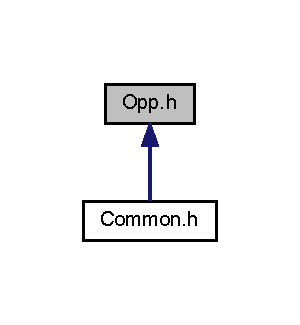
\includegraphics[width=144pt]{a00068}
\end{center}
\end{figure}
\subsection*{Macros}
\begin{DoxyCompactItemize}
\item 
\#define \hyperlink{a00032_afe8a1619d93171d3cc6de1547cb65982}{L\-O\-A\-D1\-\_\-\-O\-P\-P\-\_\-\-T\-R\-I\-P}~1
\item 
\#define \hyperlink{a00032_a2f2ad16c48f8bfdb51272ac7c001b005}{L\-O\-A\-D2\-\_\-\-O\-P\-P\-\_\-\-T\-R\-I\-P}~2
\item 
\#define \hyperlink{a00032_afb895ec8b4e74e28a73708371b75cdb7}{L\-O\-A\-D3\-\_\-\-O\-P\-P\-\_\-\-T\-R\-I\-P}~4
\item 
\#define \hyperlink{a00032_afb8941d83fb2ddbdf96fdf7ac8f5d259}{L\-O\-A\-D4\-\_\-\-O\-P\-P\-\_\-\-T\-R\-I\-P}~8
\item 
\#define \hyperlink{a00032_ac02d3bbcf9e07f26248ae2f667713770}{D\-C\-M\-I\-D\-\_\-\-O\-P\-P\-\_\-\-T\-R\-I\-P}~16
\item 
\#define \hyperlink{a00032_af157ad216f4a380ac6db0b81cb384e4a}{D\-C\-H\-V\-\_\-\-O\-P\-P\-\_\-\-T\-R\-I\-P}~32
\item 
\#define \hyperlink{a00032_adf494b474f7ddb554f7d6095fa5bf387}{A\-C\-\_\-\-O\-P\-P\-\_\-\-T\-R\-I\-P}~64
\end{DoxyCompactItemize}
\subsection*{Functions}
\begin{DoxyCompactItemize}
\item 
Uint16 \hyperlink{a00032_ad66082246819b4aa7758cb791de55ca2}{check\-Load\-Opp} (\hyperlink{a00027_a2820f1e18d921d2f1e97d53404b9fbae}{load\-Stage} load)
\item 
Uint16 \hyperlink{a00032_afc7fb5a768a0ddaf7e99dd65eb84a3b0}{get\-Load\-Opp\-State} (\hyperlink{a00027_a2820f1e18d921d2f1e97d53404b9fbae}{load\-Stage} load)
\item 
Uint16 \hyperlink{a00032_a16c41a7ea9c7037ab8721ea914269e71}{clear\-Load\-Opp} (\hyperlink{a00027_a2820f1e18d921d2f1e97d53404b9fbae}{load\-Stage} load)
\item 
Uint16 \hyperlink{a00032_aaaf0cea838afd7187715dc2a84e644f3}{check\-Ac\-Opp} (void)
\item 
Uint16 \hyperlink{a00032_a6b586bb208ca60bcbfc630685df47bf0}{get\-Ac\-Opp\-State} (void)
\item 
Uint16 \hyperlink{a00032_af4e230aa537a2cc7cb6daa364fabaca9}{clear\-Ac\-Opp} (void)
\end{DoxyCompactItemize}


\subsection{Detailed Description}
Over-\/power protection functions. These functions require that the relevant relevant measurement scales be set before use. 

\subsection{Macro Definition Documentation}
\hypertarget{a00032_adf494b474f7ddb554f7d6095fa5bf387}{\index{Opp.\-h@{Opp.\-h}!A\-C\-\_\-\-O\-P\-P\-\_\-\-T\-R\-I\-P@{A\-C\-\_\-\-O\-P\-P\-\_\-\-T\-R\-I\-P}}
\index{A\-C\-\_\-\-O\-P\-P\-\_\-\-T\-R\-I\-P@{A\-C\-\_\-\-O\-P\-P\-\_\-\-T\-R\-I\-P}!Opp.h@{Opp.\-h}}
\subsubsection[{A\-C\-\_\-\-O\-P\-P\-\_\-\-T\-R\-I\-P}]{\setlength{\rightskip}{0pt plus 5cm}\#define A\-C\-\_\-\-O\-P\-P\-\_\-\-T\-R\-I\-P~64}}\label{a00032_adf494b474f7ddb554f7d6095fa5bf387}
O\-P\-P flag register A\-C bit. \hypertarget{a00032_af157ad216f4a380ac6db0b81cb384e4a}{\index{Opp.\-h@{Opp.\-h}!D\-C\-H\-V\-\_\-\-O\-P\-P\-\_\-\-T\-R\-I\-P@{D\-C\-H\-V\-\_\-\-O\-P\-P\-\_\-\-T\-R\-I\-P}}
\index{D\-C\-H\-V\-\_\-\-O\-P\-P\-\_\-\-T\-R\-I\-P@{D\-C\-H\-V\-\_\-\-O\-P\-P\-\_\-\-T\-R\-I\-P}!Opp.h@{Opp.\-h}}
\subsubsection[{D\-C\-H\-V\-\_\-\-O\-P\-P\-\_\-\-T\-R\-I\-P}]{\setlength{\rightskip}{0pt plus 5cm}\#define D\-C\-H\-V\-\_\-\-O\-P\-P\-\_\-\-T\-R\-I\-P~32}}\label{a00032_af157ad216f4a380ac6db0b81cb384e4a}
O\-P\-P flag register D\-C H\-V bit. \hypertarget{a00032_ac02d3bbcf9e07f26248ae2f667713770}{\index{Opp.\-h@{Opp.\-h}!D\-C\-M\-I\-D\-\_\-\-O\-P\-P\-\_\-\-T\-R\-I\-P@{D\-C\-M\-I\-D\-\_\-\-O\-P\-P\-\_\-\-T\-R\-I\-P}}
\index{D\-C\-M\-I\-D\-\_\-\-O\-P\-P\-\_\-\-T\-R\-I\-P@{D\-C\-M\-I\-D\-\_\-\-O\-P\-P\-\_\-\-T\-R\-I\-P}!Opp.h@{Opp.\-h}}
\subsubsection[{D\-C\-M\-I\-D\-\_\-\-O\-P\-P\-\_\-\-T\-R\-I\-P}]{\setlength{\rightskip}{0pt plus 5cm}\#define D\-C\-M\-I\-D\-\_\-\-O\-P\-P\-\_\-\-T\-R\-I\-P~16}}\label{a00032_ac02d3bbcf9e07f26248ae2f667713770}
O\-P\-P flag register D\-C M\-I\-D bit. \hypertarget{a00032_afe8a1619d93171d3cc6de1547cb65982}{\index{Opp.\-h@{Opp.\-h}!L\-O\-A\-D1\-\_\-\-O\-P\-P\-\_\-\-T\-R\-I\-P@{L\-O\-A\-D1\-\_\-\-O\-P\-P\-\_\-\-T\-R\-I\-P}}
\index{L\-O\-A\-D1\-\_\-\-O\-P\-P\-\_\-\-T\-R\-I\-P@{L\-O\-A\-D1\-\_\-\-O\-P\-P\-\_\-\-T\-R\-I\-P}!Opp.h@{Opp.\-h}}
\subsubsection[{L\-O\-A\-D1\-\_\-\-O\-P\-P\-\_\-\-T\-R\-I\-P}]{\setlength{\rightskip}{0pt plus 5cm}\#define L\-O\-A\-D1\-\_\-\-O\-P\-P\-\_\-\-T\-R\-I\-P~1}}\label{a00032_afe8a1619d93171d3cc6de1547cb65982}
O\-P\-P flag register load 1 bit. \hypertarget{a00032_a2f2ad16c48f8bfdb51272ac7c001b005}{\index{Opp.\-h@{Opp.\-h}!L\-O\-A\-D2\-\_\-\-O\-P\-P\-\_\-\-T\-R\-I\-P@{L\-O\-A\-D2\-\_\-\-O\-P\-P\-\_\-\-T\-R\-I\-P}}
\index{L\-O\-A\-D2\-\_\-\-O\-P\-P\-\_\-\-T\-R\-I\-P@{L\-O\-A\-D2\-\_\-\-O\-P\-P\-\_\-\-T\-R\-I\-P}!Opp.h@{Opp.\-h}}
\subsubsection[{L\-O\-A\-D2\-\_\-\-O\-P\-P\-\_\-\-T\-R\-I\-P}]{\setlength{\rightskip}{0pt plus 5cm}\#define L\-O\-A\-D2\-\_\-\-O\-P\-P\-\_\-\-T\-R\-I\-P~2}}\label{a00032_a2f2ad16c48f8bfdb51272ac7c001b005}
O\-P\-P flag register load 2 bit. \hypertarget{a00032_afb895ec8b4e74e28a73708371b75cdb7}{\index{Opp.\-h@{Opp.\-h}!L\-O\-A\-D3\-\_\-\-O\-P\-P\-\_\-\-T\-R\-I\-P@{L\-O\-A\-D3\-\_\-\-O\-P\-P\-\_\-\-T\-R\-I\-P}}
\index{L\-O\-A\-D3\-\_\-\-O\-P\-P\-\_\-\-T\-R\-I\-P@{L\-O\-A\-D3\-\_\-\-O\-P\-P\-\_\-\-T\-R\-I\-P}!Opp.h@{Opp.\-h}}
\subsubsection[{L\-O\-A\-D3\-\_\-\-O\-P\-P\-\_\-\-T\-R\-I\-P}]{\setlength{\rightskip}{0pt plus 5cm}\#define L\-O\-A\-D3\-\_\-\-O\-P\-P\-\_\-\-T\-R\-I\-P~4}}\label{a00032_afb895ec8b4e74e28a73708371b75cdb7}
O\-P\-P flag register load 3 bit. \hypertarget{a00032_afb8941d83fb2ddbdf96fdf7ac8f5d259}{\index{Opp.\-h@{Opp.\-h}!L\-O\-A\-D4\-\_\-\-O\-P\-P\-\_\-\-T\-R\-I\-P@{L\-O\-A\-D4\-\_\-\-O\-P\-P\-\_\-\-T\-R\-I\-P}}
\index{L\-O\-A\-D4\-\_\-\-O\-P\-P\-\_\-\-T\-R\-I\-P@{L\-O\-A\-D4\-\_\-\-O\-P\-P\-\_\-\-T\-R\-I\-P}!Opp.h@{Opp.\-h}}
\subsubsection[{L\-O\-A\-D4\-\_\-\-O\-P\-P\-\_\-\-T\-R\-I\-P}]{\setlength{\rightskip}{0pt plus 5cm}\#define L\-O\-A\-D4\-\_\-\-O\-P\-P\-\_\-\-T\-R\-I\-P~8}}\label{a00032_afb8941d83fb2ddbdf96fdf7ac8f5d259}
O\-P\-P flag register load 4 bit. 

\subsection{Function Documentation}
\hypertarget{a00032_aaaf0cea838afd7187715dc2a84e644f3}{\index{Opp.\-h@{Opp.\-h}!check\-Ac\-Opp@{check\-Ac\-Opp}}
\index{check\-Ac\-Opp@{check\-Ac\-Opp}!Opp.h@{Opp.\-h}}
\subsubsection[{check\-Ac\-Opp}]{\setlength{\rightskip}{0pt plus 5cm}Uint16 check\-Ac\-Opp (
\begin{DoxyParamCaption}
\item[{void}]{}
\end{DoxyParamCaption}
)}}\label{a00032_aaaf0cea838afd7187715dc2a84e644f3}
Checks the current reading of the A\-C stage against the A\-C O\-P\-P limit. Raises the A\-C O\-P\-P flag if the reading is above the limit. \begin{DoxyReturn}{Returns}
Error status 
\end{DoxyReturn}
\hypertarget{a00032_ad66082246819b4aa7758cb791de55ca2}{\index{Opp.\-h@{Opp.\-h}!check\-Load\-Opp@{check\-Load\-Opp}}
\index{check\-Load\-Opp@{check\-Load\-Opp}!Opp.h@{Opp.\-h}}
\subsubsection[{check\-Load\-Opp}]{\setlength{\rightskip}{0pt plus 5cm}Uint16 check\-Load\-Opp (
\begin{DoxyParamCaption}
\item[{{\bf load\-Stage}}]{load}
\end{DoxyParamCaption}
)}}\label{a00032_ad66082246819b4aa7758cb791de55ca2}
$<$ O\-P\-P flag register. Bits are set to indicate an O\-P\-P condition has been found. Checks the power reading of the specified load against the load O\-P\-P limit. Raises the load O\-P\-P flag if the reading is above the limit. 
\begin{DoxyParams}[1]{Parameters}
\mbox{\tt in}  & {\em load} & Specifies the load on which the reading is to be tested. \\
\hline
\end{DoxyParams}
\begin{DoxyReturn}{Returns}
Error status 
\end{DoxyReturn}
\hypertarget{a00032_af4e230aa537a2cc7cb6daa364fabaca9}{\index{Opp.\-h@{Opp.\-h}!clear\-Ac\-Opp@{clear\-Ac\-Opp}}
\index{clear\-Ac\-Opp@{clear\-Ac\-Opp}!Opp.h@{Opp.\-h}}
\subsubsection[{clear\-Ac\-Opp}]{\setlength{\rightskip}{0pt plus 5cm}Uint16 clear\-Ac\-Opp (
\begin{DoxyParamCaption}
\item[{void}]{}
\end{DoxyParamCaption}
)}}\label{a00032_af4e230aa537a2cc7cb6daa364fabaca9}
Clears the A\-C stage O\-P\-P state. \begin{DoxyReturn}{Returns}
Error status. 
\end{DoxyReturn}
\hypertarget{a00032_a16c41a7ea9c7037ab8721ea914269e71}{\index{Opp.\-h@{Opp.\-h}!clear\-Load\-Opp@{clear\-Load\-Opp}}
\index{clear\-Load\-Opp@{clear\-Load\-Opp}!Opp.h@{Opp.\-h}}
\subsubsection[{clear\-Load\-Opp}]{\setlength{\rightskip}{0pt plus 5cm}Uint16 clear\-Load\-Opp (
\begin{DoxyParamCaption}
\item[{{\bf load\-Stage}}]{load}
\end{DoxyParamCaption}
)}}\label{a00032_a16c41a7ea9c7037ab8721ea914269e71}
Clears the O\-P\-P state for the specified load. 
\begin{DoxyParams}[1]{Parameters}
\mbox{\tt in}  & {\em load} & Specifies the load for which the O\-P\-P state is to be cleared. \\
\hline
\end{DoxyParams}
\begin{DoxyReturn}{Returns}
Error status. 
\end{DoxyReturn}
\hypertarget{a00032_a6b586bb208ca60bcbfc630685df47bf0}{\index{Opp.\-h@{Opp.\-h}!get\-Ac\-Opp\-State@{get\-Ac\-Opp\-State}}
\index{get\-Ac\-Opp\-State@{get\-Ac\-Opp\-State}!Opp.h@{Opp.\-h}}
\subsubsection[{get\-Ac\-Opp\-State}]{\setlength{\rightskip}{0pt plus 5cm}Uint16 get\-Ac\-Opp\-State (
\begin{DoxyParamCaption}
\item[{void}]{}
\end{DoxyParamCaption}
)}}\label{a00032_a6b586bb208ca60bcbfc630685df47bf0}
Queries the state of the A\-C O\-P\-P flag. \begin{DoxyReturn}{Returns}
True if O\-P\-P flag has been raised. 
\end{DoxyReturn}
\hypertarget{a00032_afc7fb5a768a0ddaf7e99dd65eb84a3b0}{\index{Opp.\-h@{Opp.\-h}!get\-Load\-Opp\-State@{get\-Load\-Opp\-State}}
\index{get\-Load\-Opp\-State@{get\-Load\-Opp\-State}!Opp.h@{Opp.\-h}}
\subsubsection[{get\-Load\-Opp\-State}]{\setlength{\rightskip}{0pt plus 5cm}Uint16 get\-Load\-Opp\-State (
\begin{DoxyParamCaption}
\item[{{\bf load\-Stage}}]{load}
\end{DoxyParamCaption}
)}}\label{a00032_afc7fb5a768a0ddaf7e99dd65eb84a3b0}
Queries the state of the O\-P\-P flag for the specified load. 
\begin{DoxyParams}[1]{Parameters}
\mbox{\tt in}  & {\em load} & Specifies the load on which to check the flag. \\
\hline
\end{DoxyParams}
\begin{DoxyReturn}{Returns}
True if O\-P\-P flag has been raised. 
\end{DoxyReturn}

\hypertarget{a00034}{\section{Slew\-Control.\-h File Reference}
\label{a00034}\index{Slew\-Control.\-h@{Slew\-Control.\-h}}
}


Slew control functions.  


This graph shows which files directly or indirectly include this file\-:
\nopagebreak
\begin{figure}[H]
\begin{center}
\leavevmode
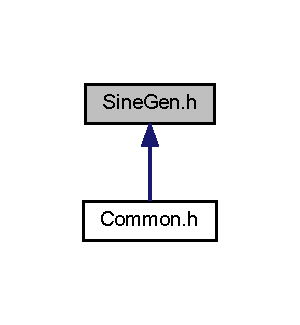
\includegraphics[width=156pt]{a00056}
\end{center}
\end{figure}
\subsection*{Functions}
\begin{DoxyCompactItemize}
\item 
void \hyperlink{a00034_a8f8f2b1ef59b7fa90122e5609e24cd06}{sc\-Slew\-Update} (void)
\item 
Uint16 \hyperlink{a00034_acd4f1d77c353f333438ae688a9bcc8fe}{sc\-Set\-Target} (Uint16 chnl, float32 trgt)
\item 
Uint16 \hyperlink{a00034_a91e197a77f8f6c05dc478431164114a4}{sc\-Set\-Step} (Uint16 chnl, float32 stp)
\item 
Uint16 \hyperlink{a00034_a92578a062af02eb967ca2dfbd68b00cf}{sc\-Set\-State} (Uint16 chnl, Uint16 stt)
\item 
Uint16 \hyperlink{a00034_a1e7d07e1a6d9b1e40b1b39d97df638b9}{sc\-Set\-Target\-All} (float32 trgt)
\item 
Uint16 \hyperlink{a00034_a2dbe145695a65570ebc1ff5588e08a18}{sc\-Set\-Step\-All} (float32 stp)
\item 
Uint16 \hyperlink{a00034_af4b016a1a10639dfeca7af4f750d8c75}{sc\-Set\-State\-All} (Uint16 stt)
\item 
Uint16 \hyperlink{a00034_ab83b8f320a4bf9e8ea1a251fec458032}{sc\-Get\-Target} (Uint16 chnl, float32 $\ast$trgt\-Dest)
\item 
Uint16 \hyperlink{a00034_adac64f58de9a029d849e0df2962bad16}{sc\-Get\-Step} (Uint16 chnl, float32 $\ast$stp\-Dest)
\item 
Uint16 \hyperlink{a00034_a77a235d70df3aff6a742ff375bd45119}{sc\-Get\-State} (Uint16 chnl, Uint16 $\ast$stt\-Dest)
\end{DoxyCompactItemize}


\subsection{Detailed Description}
Slew control functions. 

\subsection{Function Documentation}
\hypertarget{a00034_a77a235d70df3aff6a742ff375bd45119}{\index{Slew\-Control.\-h@{Slew\-Control.\-h}!sc\-Get\-State@{sc\-Get\-State}}
\index{sc\-Get\-State@{sc\-Get\-State}!SlewControl.h@{Slew\-Control.\-h}}
\subsubsection[{sc\-Get\-State}]{\setlength{\rightskip}{0pt plus 5cm}Uint16 sc\-Get\-State (
\begin{DoxyParamCaption}
\item[{Uint16}]{chnl, }
\item[{Uint16 $\ast$}]{stt\-Dest}
\end{DoxyParamCaption}
)}}\label{a00034_a77a235d70df3aff6a742ff375bd45119}
Queries the current reference net enable state for the specified channel. 
\begin{DoxyParams}[1]{Parameters}
\mbox{\tt in}  & {\em chnl} & Specifies the channel the setting is to be read from. \\
\hline
\mbox{\tt out}  & {\em stt\-Dest} & Address of the memory location at which to place the query result (0\-:O\-F\-F $|$ non-\/zero\-:O\-N). \\
\hline
\end{DoxyParams}
\begin{DoxyReturn}{Returns}
Error status. 
\end{DoxyReturn}
\hypertarget{a00034_adac64f58de9a029d849e0df2962bad16}{\index{Slew\-Control.\-h@{Slew\-Control.\-h}!sc\-Get\-Step@{sc\-Get\-Step}}
\index{sc\-Get\-Step@{sc\-Get\-Step}!SlewControl.h@{Slew\-Control.\-h}}
\subsubsection[{sc\-Get\-Step}]{\setlength{\rightskip}{0pt plus 5cm}Uint16 sc\-Get\-Step (
\begin{DoxyParamCaption}
\item[{Uint16}]{chnl, }
\item[{float32 $\ast$}]{stp\-Dest}
\end{DoxyParamCaption}
)}}\label{a00034_adac64f58de9a029d849e0df2962bad16}
Queries the current slew step size of the specified channel. 
\begin{DoxyParams}[1]{Parameters}
\mbox{\tt in}  & {\em chnl} & Specifies the channel the setting is to be read from. \\
\hline
\mbox{\tt out}  & {\em stp\-Dest} & Address of the memory location at which to place the query result (amps or volts). \\
\hline
\end{DoxyParams}
\begin{DoxyReturn}{Returns}
Error status. 
\end{DoxyReturn}
\hypertarget{a00034_ab83b8f320a4bf9e8ea1a251fec458032}{\index{Slew\-Control.\-h@{Slew\-Control.\-h}!sc\-Get\-Target@{sc\-Get\-Target}}
\index{sc\-Get\-Target@{sc\-Get\-Target}!SlewControl.h@{Slew\-Control.\-h}}
\subsubsection[{sc\-Get\-Target}]{\setlength{\rightskip}{0pt plus 5cm}Uint16 sc\-Get\-Target (
\begin{DoxyParamCaption}
\item[{Uint16}]{chnl, }
\item[{float32 $\ast$}]{trgt\-Dest}
\end{DoxyParamCaption}
)}}\label{a00034_ab83b8f320a4bf9e8ea1a251fec458032}
Queries the current slew target setting for the specified channel. 
\begin{DoxyParams}[1]{Parameters}
\mbox{\tt in}  & {\em chnl} & Specifies the channel the setting is to be read from. \\
\hline
\mbox{\tt out}  & {\em trgt\-Dest} & Address of the memory location at which to place the query result (amps or volts). \\
\hline
\end{DoxyParams}
\begin{DoxyReturn}{Returns}
Error status. 
\end{DoxyReturn}
\hypertarget{a00034_a92578a062af02eb967ca2dfbd68b00cf}{\index{Slew\-Control.\-h@{Slew\-Control.\-h}!sc\-Set\-State@{sc\-Set\-State}}
\index{sc\-Set\-State@{sc\-Set\-State}!SlewControl.h@{Slew\-Control.\-h}}
\subsubsection[{sc\-Set\-State}]{\setlength{\rightskip}{0pt plus 5cm}Uint16 sc\-Set\-State (
\begin{DoxyParamCaption}
\item[{Uint16}]{chnl, }
\item[{Uint16}]{stt}
\end{DoxyParamCaption}
)}}\label{a00034_a92578a062af02eb967ca2dfbd68b00cf}
Sets the reference net enable state for the specified channel. 
\begin{DoxyParams}[1]{Parameters}
\mbox{\tt in}  & {\em chnl} & Specifies the channel the setting is to be applied to. \\
\hline
\mbox{\tt in}  & {\em stt} & Specifies the reference net state to be applied (0\-:O\-F\-F $|$ non-\/zero\-:O\-N). \\
\hline
\end{DoxyParams}
\begin{DoxyReturn}{Returns}
Error Status. 
\end{DoxyReturn}
\hypertarget{a00034_af4b016a1a10639dfeca7af4f750d8c75}{\index{Slew\-Control.\-h@{Slew\-Control.\-h}!sc\-Set\-State\-All@{sc\-Set\-State\-All}}
\index{sc\-Set\-State\-All@{sc\-Set\-State\-All}!SlewControl.h@{Slew\-Control.\-h}}
\subsubsection[{sc\-Set\-State\-All}]{\setlength{\rightskip}{0pt plus 5cm}Uint16 sc\-Set\-State\-All (
\begin{DoxyParamCaption}
\item[{Uint16}]{stt}
\end{DoxyParamCaption}
)}}\label{a00034_af4b016a1a10639dfeca7af4f750d8c75}
Sets all channels' reference net enable state. 
\begin{DoxyParams}[1]{Parameters}
\mbox{\tt in}  & {\em stt} & Specifies the refernce net state to be applied (0\-:O\-F\-F $|$ non-\/zero\-:O\-N). \\
\hline
\end{DoxyParams}
\begin{DoxyReturn}{Returns}
Error status. 
\end{DoxyReturn}
\hypertarget{a00034_a91e197a77f8f6c05dc478431164114a4}{\index{Slew\-Control.\-h@{Slew\-Control.\-h}!sc\-Set\-Step@{sc\-Set\-Step}}
\index{sc\-Set\-Step@{sc\-Set\-Step}!SlewControl.h@{Slew\-Control.\-h}}
\subsubsection[{sc\-Set\-Step}]{\setlength{\rightskip}{0pt plus 5cm}Uint16 sc\-Set\-Step (
\begin{DoxyParamCaption}
\item[{Uint16}]{chnl, }
\item[{float32}]{stp}
\end{DoxyParamCaption}
)}}\label{a00034_a91e197a77f8f6c05dc478431164114a4}
Sets the slew step size for the specified channel. 
\begin{DoxyParams}[1]{Parameters}
\mbox{\tt in}  & {\em chnl} & Specifies the channel the setting is to be applied to. \\
\hline
\mbox{\tt in}  & {\em stp} & Specifies the value of the slew step size to be applied (amps or volts). \\
\hline
\end{DoxyParams}
\begin{DoxyReturn}{Returns}
Error status. 
\end{DoxyReturn}
\hypertarget{a00034_a2dbe145695a65570ebc1ff5588e08a18}{\index{Slew\-Control.\-h@{Slew\-Control.\-h}!sc\-Set\-Step\-All@{sc\-Set\-Step\-All}}
\index{sc\-Set\-Step\-All@{sc\-Set\-Step\-All}!SlewControl.h@{Slew\-Control.\-h}}
\subsubsection[{sc\-Set\-Step\-All}]{\setlength{\rightskip}{0pt plus 5cm}Uint16 sc\-Set\-Step\-All (
\begin{DoxyParamCaption}
\item[{float32}]{stp}
\end{DoxyParamCaption}
)}}\label{a00034_a2dbe145695a65570ebc1ff5588e08a18}
Sets all channels' slew step size. 
\begin{DoxyParams}[1]{Parameters}
\mbox{\tt in}  & {\em stp} & Specifies the value of the slew step size to be applied (amps or volts). \\
\hline
\end{DoxyParams}
\begin{DoxyReturn}{Returns}
Error status. 
\end{DoxyReturn}
\hypertarget{a00034_acd4f1d77c353f333438ae688a9bcc8fe}{\index{Slew\-Control.\-h@{Slew\-Control.\-h}!sc\-Set\-Target@{sc\-Set\-Target}}
\index{sc\-Set\-Target@{sc\-Set\-Target}!SlewControl.h@{Slew\-Control.\-h}}
\subsubsection[{sc\-Set\-Target}]{\setlength{\rightskip}{0pt plus 5cm}Uint16 sc\-Set\-Target (
\begin{DoxyParamCaption}
\item[{Uint16}]{chnl, }
\item[{float32}]{trgt}
\end{DoxyParamCaption}
)}}\label{a00034_acd4f1d77c353f333438ae688a9bcc8fe}
Sets the slew target for the specified channel. 
\begin{DoxyParams}[1]{Parameters}
\mbox{\tt in}  & {\em chnl} & Specifies the channel the setting is to be applied to. \\
\hline
\mbox{\tt in}  & {\em trgt} & Specifies the value of the slew target to be applied (amps or volts). \\
\hline
\end{DoxyParams}
\begin{DoxyReturn}{Returns}
Error status. 
\end{DoxyReturn}
\hypertarget{a00034_a1e7d07e1a6d9b1e40b1b39d97df638b9}{\index{Slew\-Control.\-h@{Slew\-Control.\-h}!sc\-Set\-Target\-All@{sc\-Set\-Target\-All}}
\index{sc\-Set\-Target\-All@{sc\-Set\-Target\-All}!SlewControl.h@{Slew\-Control.\-h}}
\subsubsection[{sc\-Set\-Target\-All}]{\setlength{\rightskip}{0pt plus 5cm}Uint16 sc\-Set\-Target\-All (
\begin{DoxyParamCaption}
\item[{float32}]{trgt}
\end{DoxyParamCaption}
)}}\label{a00034_a1e7d07e1a6d9b1e40b1b39d97df638b9}
Sets all channels' slew target 
\begin{DoxyParams}[1]{Parameters}
\mbox{\tt in}  & {\em trgt} & Specifies the value of the slew target to be applied (amps or volts). \\
\hline
\end{DoxyParams}
\begin{DoxyReturn}{Returns}
Error status. 
\end{DoxyReturn}
\hypertarget{a00034_a8f8f2b1ef59b7fa90122e5609e24cd06}{\index{Slew\-Control.\-h@{Slew\-Control.\-h}!sc\-Slew\-Update@{sc\-Slew\-Update}}
\index{sc\-Slew\-Update@{sc\-Slew\-Update}!SlewControl.h@{Slew\-Control.\-h}}
\subsubsection[{sc\-Slew\-Update}]{\setlength{\rightskip}{0pt plus 5cm}void sc\-Slew\-Update (
\begin{DoxyParamCaption}
\item[{void}]{}
\end{DoxyParamCaption}
)}}\label{a00034_a8f8f2b1ef59b7fa90122e5609e24cd06}
Advances the slew ramps for all relevant channels. Does not apply to channels that use sine references 
\hypertarget{a00036}{\section{Ovp.\-h File Reference}
\label{a00036}\index{Ovp.\-h@{Ovp.\-h}}
}


Over-\/voltage protection functions.  


This graph shows which files directly or indirectly include this file\-:\nopagebreak
\begin{figure}[H]
\begin{center}
\leavevmode
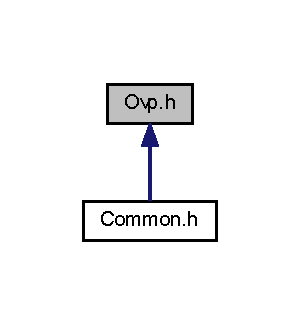
\includegraphics[width=144pt]{a00070}
\end{center}
\end{figure}
\subsection*{Macros}
\begin{DoxyCompactItemize}
\item 
\#define \hyperlink{a00036_a818e48bd3796e85aff1e441d395d420e}{L\-O\-A\-D1\-\_\-\-O\-V\-P\-\_\-\-T\-R\-I\-P}~1
\item 
\#define \hyperlink{a00036_a06deb869d76201f8fa804f155a6d0204}{L\-O\-A\-D2\-\_\-\-O\-V\-P\-\_\-\-T\-R\-I\-P}~2
\item 
\#define \hyperlink{a00036_a48d28ba735dc28df3ba0c96ca99c3ba0}{L\-O\-A\-D3\-\_\-\-O\-V\-P\-\_\-\-T\-R\-I\-P}~4
\item 
\#define \hyperlink{a00036_a77c2bd0f4f1081fadf180ae92c5b0b79}{L\-O\-A\-D4\-\_\-\-O\-V\-P\-\_\-\-T\-R\-I\-P}~8
\item 
\#define \hyperlink{a00036_a454809e1e9a6314875f8f833bd924bfb}{D\-C\-M\-I\-D\-\_\-\-O\-V\-P\-\_\-\-T\-R\-I\-P}~16
\item 
\#define \hyperlink{a00036_a87d04fee238f7921a66521910b42244e}{D\-C\-H\-V\-\_\-\-O\-V\-P\-\_\-\-T\-R\-I\-P}~32
\item 
\#define \hyperlink{a00036_abf1557b371e135706243aebb018260cc}{A\-C\-\_\-\-O\-V\-P\-\_\-\-T\-R\-I\-P}~64
\end{DoxyCompactItemize}
\subsection*{Functions}
\begin{DoxyCompactItemize}
\item 
Uint16 \hyperlink{a00036_aff7629dfd95df8d951d2655a469e4f0b}{check\-Load\-Ovp} (\hyperlink{a00027_a2820f1e18d921d2f1e97d53404b9fbae}{load\-Stage} load)
\item 
Uint16 \hyperlink{a00036_afef3389418ef30049023606f8ee1e63a}{get\-Load\-Ovp\-State} (\hyperlink{a00027_a2820f1e18d921d2f1e97d53404b9fbae}{load\-Stage} load)
\item 
Uint16 \hyperlink{a00036_a90b85f0cd911b4628b2713072a755884}{clear\-Load\-Ovp} (\hyperlink{a00027_a2820f1e18d921d2f1e97d53404b9fbae}{load\-Stage} load)
\item 
Uint16 \hyperlink{a00036_ae23e841cb8641e0253b5a8aa96ef2f2e}{trip\-Dc\-Mid\-Ovp} (void)
\item 
Uint16 \hyperlink{a00036_af1c17192cdfb57ea80342583e1f25594}{get\-Dc\-Mid\-Ovp\-State} (void)
\item 
Uint16 \hyperlink{a00036_a04846ddb31daf651daeea01e6949a633}{clear\-Dc\-Mid\-Ovp} (void)
\item 
Uint16 \hyperlink{a00036_a5e4e700d4759e7f0a6289796773f8e2b}{set\-Dc\-Hv\-Ovp\-Level} (float32 dc\-Level)
\item 
Uint16 \hyperlink{a00036_a1311d68beecad9f6ffa0cf03993b6793}{get\-Dc\-Hv\-Ovp\-Level} (float32 $\ast$dc\-Level)
\item 
Uint16 \hyperlink{a00036_a88172749798c193b8081da2d6f03673e}{check\-Dc\-Hv\-Ovp} (void)
\item 
Uint16 \hyperlink{a00036_abca9d133fd7de92546ad0a332119e921}{get\-Dc\-Hv\-Ovp\-State} (void)
\item 
Uint16 \hyperlink{a00036_a466dac1e76240f74d4d50a5f2d026fdd}{clear\-Dc\-Hv\-Ovp} (void)
\item 
Uint16 \hyperlink{a00036_a93b0c8c63f03b67ac81ef674232ccfd0}{set\-Ac\-Ovp\-Level} (float32 pk\-Level)
\item 
Uint16 \hyperlink{a00036_a74d933fe7f4604bdd0a52086d6edd817}{get\-Ac\-Ovp\-Level} (float32 $\ast$pk\-Level)
\item 
Uint16 \hyperlink{a00036_aaca3e8b9f1e75b6ec31e5270c62cdd9a}{check\-Ac\-Ovp} (void)
\item 
Uint16 \hyperlink{a00036_a6b51e17f10032455c6984b20353d82b9}{get\-Ac\-Ovp\-State} (void)
\item 
Uint16 \hyperlink{a00036_a8b53919933a6e29ab7d5e3a0fccf0823}{clear\-Ac\-Ovp} (void)
\end{DoxyCompactItemize}


\subsection{Detailed Description}
Over-\/voltage protection functions. These functions require that the relevant relevant measurement scales be set before use. 

\subsection{Macro Definition Documentation}
\hypertarget{a00036_abf1557b371e135706243aebb018260cc}{\index{Ovp.\-h@{Ovp.\-h}!A\-C\-\_\-\-O\-V\-P\-\_\-\-T\-R\-I\-P@{A\-C\-\_\-\-O\-V\-P\-\_\-\-T\-R\-I\-P}}
\index{A\-C\-\_\-\-O\-V\-P\-\_\-\-T\-R\-I\-P@{A\-C\-\_\-\-O\-V\-P\-\_\-\-T\-R\-I\-P}!Ovp.h@{Ovp.\-h}}
\subsubsection[{A\-C\-\_\-\-O\-V\-P\-\_\-\-T\-R\-I\-P}]{\setlength{\rightskip}{0pt plus 5cm}\#define A\-C\-\_\-\-O\-V\-P\-\_\-\-T\-R\-I\-P~64}}\label{a00036_abf1557b371e135706243aebb018260cc}
O\-V\-P flag register A\-C bit. \hypertarget{a00036_a87d04fee238f7921a66521910b42244e}{\index{Ovp.\-h@{Ovp.\-h}!D\-C\-H\-V\-\_\-\-O\-V\-P\-\_\-\-T\-R\-I\-P@{D\-C\-H\-V\-\_\-\-O\-V\-P\-\_\-\-T\-R\-I\-P}}
\index{D\-C\-H\-V\-\_\-\-O\-V\-P\-\_\-\-T\-R\-I\-P@{D\-C\-H\-V\-\_\-\-O\-V\-P\-\_\-\-T\-R\-I\-P}!Ovp.h@{Ovp.\-h}}
\subsubsection[{D\-C\-H\-V\-\_\-\-O\-V\-P\-\_\-\-T\-R\-I\-P}]{\setlength{\rightskip}{0pt plus 5cm}\#define D\-C\-H\-V\-\_\-\-O\-V\-P\-\_\-\-T\-R\-I\-P~32}}\label{a00036_a87d04fee238f7921a66521910b42244e}
O\-V\-P flag register D\-C H\-V bit. \hypertarget{a00036_a454809e1e9a6314875f8f833bd924bfb}{\index{Ovp.\-h@{Ovp.\-h}!D\-C\-M\-I\-D\-\_\-\-O\-V\-P\-\_\-\-T\-R\-I\-P@{D\-C\-M\-I\-D\-\_\-\-O\-V\-P\-\_\-\-T\-R\-I\-P}}
\index{D\-C\-M\-I\-D\-\_\-\-O\-V\-P\-\_\-\-T\-R\-I\-P@{D\-C\-M\-I\-D\-\_\-\-O\-V\-P\-\_\-\-T\-R\-I\-P}!Ovp.h@{Ovp.\-h}}
\subsubsection[{D\-C\-M\-I\-D\-\_\-\-O\-V\-P\-\_\-\-T\-R\-I\-P}]{\setlength{\rightskip}{0pt plus 5cm}\#define D\-C\-M\-I\-D\-\_\-\-O\-V\-P\-\_\-\-T\-R\-I\-P~16}}\label{a00036_a454809e1e9a6314875f8f833bd924bfb}
O\-V\-P flag register D\-C M\-I\-D bit. \hypertarget{a00036_a818e48bd3796e85aff1e441d395d420e}{\index{Ovp.\-h@{Ovp.\-h}!L\-O\-A\-D1\-\_\-\-O\-V\-P\-\_\-\-T\-R\-I\-P@{L\-O\-A\-D1\-\_\-\-O\-V\-P\-\_\-\-T\-R\-I\-P}}
\index{L\-O\-A\-D1\-\_\-\-O\-V\-P\-\_\-\-T\-R\-I\-P@{L\-O\-A\-D1\-\_\-\-O\-V\-P\-\_\-\-T\-R\-I\-P}!Ovp.h@{Ovp.\-h}}
\subsubsection[{L\-O\-A\-D1\-\_\-\-O\-V\-P\-\_\-\-T\-R\-I\-P}]{\setlength{\rightskip}{0pt plus 5cm}\#define L\-O\-A\-D1\-\_\-\-O\-V\-P\-\_\-\-T\-R\-I\-P~1}}\label{a00036_a818e48bd3796e85aff1e441d395d420e}
O\-V\-P flag register load 1 bit. \hypertarget{a00036_a06deb869d76201f8fa804f155a6d0204}{\index{Ovp.\-h@{Ovp.\-h}!L\-O\-A\-D2\-\_\-\-O\-V\-P\-\_\-\-T\-R\-I\-P@{L\-O\-A\-D2\-\_\-\-O\-V\-P\-\_\-\-T\-R\-I\-P}}
\index{L\-O\-A\-D2\-\_\-\-O\-V\-P\-\_\-\-T\-R\-I\-P@{L\-O\-A\-D2\-\_\-\-O\-V\-P\-\_\-\-T\-R\-I\-P}!Ovp.h@{Ovp.\-h}}
\subsubsection[{L\-O\-A\-D2\-\_\-\-O\-V\-P\-\_\-\-T\-R\-I\-P}]{\setlength{\rightskip}{0pt plus 5cm}\#define L\-O\-A\-D2\-\_\-\-O\-V\-P\-\_\-\-T\-R\-I\-P~2}}\label{a00036_a06deb869d76201f8fa804f155a6d0204}
O\-V\-P flag register load 2 bit. \hypertarget{a00036_a48d28ba735dc28df3ba0c96ca99c3ba0}{\index{Ovp.\-h@{Ovp.\-h}!L\-O\-A\-D3\-\_\-\-O\-V\-P\-\_\-\-T\-R\-I\-P@{L\-O\-A\-D3\-\_\-\-O\-V\-P\-\_\-\-T\-R\-I\-P}}
\index{L\-O\-A\-D3\-\_\-\-O\-V\-P\-\_\-\-T\-R\-I\-P@{L\-O\-A\-D3\-\_\-\-O\-V\-P\-\_\-\-T\-R\-I\-P}!Ovp.h@{Ovp.\-h}}
\subsubsection[{L\-O\-A\-D3\-\_\-\-O\-V\-P\-\_\-\-T\-R\-I\-P}]{\setlength{\rightskip}{0pt plus 5cm}\#define L\-O\-A\-D3\-\_\-\-O\-V\-P\-\_\-\-T\-R\-I\-P~4}}\label{a00036_a48d28ba735dc28df3ba0c96ca99c3ba0}
O\-V\-P flag register load 3 bit. \hypertarget{a00036_a77c2bd0f4f1081fadf180ae92c5b0b79}{\index{Ovp.\-h@{Ovp.\-h}!L\-O\-A\-D4\-\_\-\-O\-V\-P\-\_\-\-T\-R\-I\-P@{L\-O\-A\-D4\-\_\-\-O\-V\-P\-\_\-\-T\-R\-I\-P}}
\index{L\-O\-A\-D4\-\_\-\-O\-V\-P\-\_\-\-T\-R\-I\-P@{L\-O\-A\-D4\-\_\-\-O\-V\-P\-\_\-\-T\-R\-I\-P}!Ovp.h@{Ovp.\-h}}
\subsubsection[{L\-O\-A\-D4\-\_\-\-O\-V\-P\-\_\-\-T\-R\-I\-P}]{\setlength{\rightskip}{0pt plus 5cm}\#define L\-O\-A\-D4\-\_\-\-O\-V\-P\-\_\-\-T\-R\-I\-P~8}}\label{a00036_a77c2bd0f4f1081fadf180ae92c5b0b79}
O\-V\-P flag register load 4 bit. 

\subsection{Function Documentation}
\hypertarget{a00036_aaca3e8b9f1e75b6ec31e5270c62cdd9a}{\index{Ovp.\-h@{Ovp.\-h}!check\-Ac\-Ovp@{check\-Ac\-Ovp}}
\index{check\-Ac\-Ovp@{check\-Ac\-Ovp}!Ovp.h@{Ovp.\-h}}
\subsubsection[{check\-Ac\-Ovp}]{\setlength{\rightskip}{0pt plus 5cm}Uint16 check\-Ac\-Ovp (
\begin{DoxyParamCaption}
\item[{void}]{}
\end{DoxyParamCaption}
)}}\label{a00036_aaca3e8b9f1e75b6ec31e5270c62cdd9a}
Checks the voltage reading of the A\-C stage against the A\-C O\-V\-P limit. Raises the A\-C O\-V\-P flag if the reading is above the limit. \begin{DoxyReturn}{Returns}
Error status 
\end{DoxyReturn}
\hypertarget{a00036_a88172749798c193b8081da2d6f03673e}{\index{Ovp.\-h@{Ovp.\-h}!check\-Dc\-Hv\-Ovp@{check\-Dc\-Hv\-Ovp}}
\index{check\-Dc\-Hv\-Ovp@{check\-Dc\-Hv\-Ovp}!Ovp.h@{Ovp.\-h}}
\subsubsection[{check\-Dc\-Hv\-Ovp}]{\setlength{\rightskip}{0pt plus 5cm}Uint16 check\-Dc\-Hv\-Ovp (
\begin{DoxyParamCaption}
\item[{void}]{}
\end{DoxyParamCaption}
)}}\label{a00036_a88172749798c193b8081da2d6f03673e}
Checks the voltage reading of the D\-C H\-V stage against the D\-C H\-V O\-V\-P limit. Raises the D\-C H\-V O\-V\-P flag if the reading is above the limit. \begin{DoxyReturn}{Returns}
Error status 
\end{DoxyReturn}
\hypertarget{a00036_aff7629dfd95df8d951d2655a469e4f0b}{\index{Ovp.\-h@{Ovp.\-h}!check\-Load\-Ovp@{check\-Load\-Ovp}}
\index{check\-Load\-Ovp@{check\-Load\-Ovp}!Ovp.h@{Ovp.\-h}}
\subsubsection[{check\-Load\-Ovp}]{\setlength{\rightskip}{0pt plus 5cm}Uint16 check\-Load\-Ovp (
\begin{DoxyParamCaption}
\item[{{\bf load\-Stage}}]{load}
\end{DoxyParamCaption}
)}}\label{a00036_aff7629dfd95df8d951d2655a469e4f0b}
$<$ O\-V\-P flag register. Bits are set to indicate an O\-V\-P condition has been found. Checks the voltage reading of the specified load against the load O\-V\-P limit. Raises the load O\-V\-P flag if the reading is above the limit. 
\begin{DoxyParams}[1]{Parameters}
\mbox{\tt in}  & {\em load} & Specifies the load on which the reading is to be tested. \\
\hline
\end{DoxyParams}
\begin{DoxyReturn}{Returns}
Error status 
\end{DoxyReturn}
\hypertarget{a00036_a8b53919933a6e29ab7d5e3a0fccf0823}{\index{Ovp.\-h@{Ovp.\-h}!clear\-Ac\-Ovp@{clear\-Ac\-Ovp}}
\index{clear\-Ac\-Ovp@{clear\-Ac\-Ovp}!Ovp.h@{Ovp.\-h}}
\subsubsection[{clear\-Ac\-Ovp}]{\setlength{\rightskip}{0pt plus 5cm}Uint16 clear\-Ac\-Ovp (
\begin{DoxyParamCaption}
\item[{void}]{}
\end{DoxyParamCaption}
)}}\label{a00036_a8b53919933a6e29ab7d5e3a0fccf0823}
Clears the A\-C stage O\-V\-P state. \begin{DoxyReturn}{Returns}
Error status. 
\end{DoxyReturn}
\hypertarget{a00036_a466dac1e76240f74d4d50a5f2d026fdd}{\index{Ovp.\-h@{Ovp.\-h}!clear\-Dc\-Hv\-Ovp@{clear\-Dc\-Hv\-Ovp}}
\index{clear\-Dc\-Hv\-Ovp@{clear\-Dc\-Hv\-Ovp}!Ovp.h@{Ovp.\-h}}
\subsubsection[{clear\-Dc\-Hv\-Ovp}]{\setlength{\rightskip}{0pt plus 5cm}Uint16 clear\-Dc\-Hv\-Ovp (
\begin{DoxyParamCaption}
\item[{void}]{}
\end{DoxyParamCaption}
)}}\label{a00036_a466dac1e76240f74d4d50a5f2d026fdd}
Clears the D\-C H\-V stage O\-V\-P state. \begin{DoxyReturn}{Returns}
Error status. 
\end{DoxyReturn}
\hypertarget{a00036_a04846ddb31daf651daeea01e6949a633}{\index{Ovp.\-h@{Ovp.\-h}!clear\-Dc\-Mid\-Ovp@{clear\-Dc\-Mid\-Ovp}}
\index{clear\-Dc\-Mid\-Ovp@{clear\-Dc\-Mid\-Ovp}!Ovp.h@{Ovp.\-h}}
\subsubsection[{clear\-Dc\-Mid\-Ovp}]{\setlength{\rightskip}{0pt plus 5cm}Uint16 clear\-Dc\-Mid\-Ovp (
\begin{DoxyParamCaption}
\item[{void}]{}
\end{DoxyParamCaption}
)}}\label{a00036_a04846ddb31daf651daeea01e6949a633}
Clears the D\-C Mid stage O\-V\-P state. \begin{DoxyReturn}{Returns}
Error status. 
\end{DoxyReturn}
\hypertarget{a00036_a90b85f0cd911b4628b2713072a755884}{\index{Ovp.\-h@{Ovp.\-h}!clear\-Load\-Ovp@{clear\-Load\-Ovp}}
\index{clear\-Load\-Ovp@{clear\-Load\-Ovp}!Ovp.h@{Ovp.\-h}}
\subsubsection[{clear\-Load\-Ovp}]{\setlength{\rightskip}{0pt plus 5cm}Uint16 clear\-Load\-Ovp (
\begin{DoxyParamCaption}
\item[{{\bf load\-Stage}}]{load}
\end{DoxyParamCaption}
)}}\label{a00036_a90b85f0cd911b4628b2713072a755884}
Clears the O\-V\-P state for the specified load. 
\begin{DoxyParams}[1]{Parameters}
\mbox{\tt in}  & {\em load} & Specifies the load for which the O\-V\-P state is to be cleared. \\
\hline
\end{DoxyParams}
\begin{DoxyReturn}{Returns}
Error status. 
\end{DoxyReturn}
\hypertarget{a00036_a74d933fe7f4604bdd0a52086d6edd817}{\index{Ovp.\-h@{Ovp.\-h}!get\-Ac\-Ovp\-Level@{get\-Ac\-Ovp\-Level}}
\index{get\-Ac\-Ovp\-Level@{get\-Ac\-Ovp\-Level}!Ovp.h@{Ovp.\-h}}
\subsubsection[{get\-Ac\-Ovp\-Level}]{\setlength{\rightskip}{0pt plus 5cm}Uint16 get\-Ac\-Ovp\-Level (
\begin{DoxyParamCaption}
\item[{float32 $\ast$}]{pk\-Level}
\end{DoxyParamCaption}
)}}\label{a00036_a74d933fe7f4604bdd0a52086d6edd817}
Queries the over voltage protection level for the A\-C stage. 
\begin{DoxyParams}[1]{Parameters}
\mbox{\tt out}  & {\em pk\-Level} & Pointer to location at which to place the query result (volts). \\
\hline
\end{DoxyParams}
\begin{DoxyReturn}{Returns}
Error status. 
\end{DoxyReturn}
\hypertarget{a00036_a6b51e17f10032455c6984b20353d82b9}{\index{Ovp.\-h@{Ovp.\-h}!get\-Ac\-Ovp\-State@{get\-Ac\-Ovp\-State}}
\index{get\-Ac\-Ovp\-State@{get\-Ac\-Ovp\-State}!Ovp.h@{Ovp.\-h}}
\subsubsection[{get\-Ac\-Ovp\-State}]{\setlength{\rightskip}{0pt plus 5cm}Uint16 get\-Ac\-Ovp\-State (
\begin{DoxyParamCaption}
\item[{void}]{}
\end{DoxyParamCaption}
)}}\label{a00036_a6b51e17f10032455c6984b20353d82b9}
Queries the state of the A\-C O\-V\-P flag. \begin{DoxyReturn}{Returns}
True if O\-V\-P flag has been raised. 
\end{DoxyReturn}
\hypertarget{a00036_a1311d68beecad9f6ffa0cf03993b6793}{\index{Ovp.\-h@{Ovp.\-h}!get\-Dc\-Hv\-Ovp\-Level@{get\-Dc\-Hv\-Ovp\-Level}}
\index{get\-Dc\-Hv\-Ovp\-Level@{get\-Dc\-Hv\-Ovp\-Level}!Ovp.h@{Ovp.\-h}}
\subsubsection[{get\-Dc\-Hv\-Ovp\-Level}]{\setlength{\rightskip}{0pt plus 5cm}Uint16 get\-Dc\-Hv\-Ovp\-Level (
\begin{DoxyParamCaption}
\item[{float32 $\ast$}]{dc\-Level}
\end{DoxyParamCaption}
)}}\label{a00036_a1311d68beecad9f6ffa0cf03993b6793}
Queries the over voltage protection level for the D\-C H\-V stage. 
\begin{DoxyParams}[1]{Parameters}
\mbox{\tt out}  & {\em dc\-Level} & Pointer to location at which to place the query result (volts). \\
\hline
\end{DoxyParams}
\begin{DoxyReturn}{Returns}
Error status. 
\end{DoxyReturn}
\hypertarget{a00036_abca9d133fd7de92546ad0a332119e921}{\index{Ovp.\-h@{Ovp.\-h}!get\-Dc\-Hv\-Ovp\-State@{get\-Dc\-Hv\-Ovp\-State}}
\index{get\-Dc\-Hv\-Ovp\-State@{get\-Dc\-Hv\-Ovp\-State}!Ovp.h@{Ovp.\-h}}
\subsubsection[{get\-Dc\-Hv\-Ovp\-State}]{\setlength{\rightskip}{0pt plus 5cm}Uint16 get\-Dc\-Hv\-Ovp\-State (
\begin{DoxyParamCaption}
\item[{void}]{}
\end{DoxyParamCaption}
)}}\label{a00036_abca9d133fd7de92546ad0a332119e921}
Queries the state of the D\-C H\-V O\-V\-P flag. \begin{DoxyReturn}{Returns}
True if O\-V\-P flag has been raised. 
\end{DoxyReturn}
\hypertarget{a00036_af1c17192cdfb57ea80342583e1f25594}{\index{Ovp.\-h@{Ovp.\-h}!get\-Dc\-Mid\-Ovp\-State@{get\-Dc\-Mid\-Ovp\-State}}
\index{get\-Dc\-Mid\-Ovp\-State@{get\-Dc\-Mid\-Ovp\-State}!Ovp.h@{Ovp.\-h}}
\subsubsection[{get\-Dc\-Mid\-Ovp\-State}]{\setlength{\rightskip}{0pt plus 5cm}Uint16 get\-Dc\-Mid\-Ovp\-State (
\begin{DoxyParamCaption}
\item[{void}]{}
\end{DoxyParamCaption}
)}}\label{a00036_af1c17192cdfb57ea80342583e1f25594}
Queries the state of the D\-C Mid O\-V\-P flag. \begin{DoxyReturn}{Returns}
True if O\-V\-P flag has been raised. 
\end{DoxyReturn}
\hypertarget{a00036_afef3389418ef30049023606f8ee1e63a}{\index{Ovp.\-h@{Ovp.\-h}!get\-Load\-Ovp\-State@{get\-Load\-Ovp\-State}}
\index{get\-Load\-Ovp\-State@{get\-Load\-Ovp\-State}!Ovp.h@{Ovp.\-h}}
\subsubsection[{get\-Load\-Ovp\-State}]{\setlength{\rightskip}{0pt plus 5cm}Uint16 get\-Load\-Ovp\-State (
\begin{DoxyParamCaption}
\item[{{\bf load\-Stage}}]{load}
\end{DoxyParamCaption}
)}}\label{a00036_afef3389418ef30049023606f8ee1e63a}
Queries the state of the O\-V\-P flag for the specified load. 
\begin{DoxyParams}[1]{Parameters}
\mbox{\tt in}  & {\em load} & Specifies the load on which to check the flag. \\
\hline
\end{DoxyParams}
\begin{DoxyReturn}{Returns}
True if O\-V\-P flag has been raised. 
\end{DoxyReturn}
\hypertarget{a00036_a93b0c8c63f03b67ac81ef674232ccfd0}{\index{Ovp.\-h@{Ovp.\-h}!set\-Ac\-Ovp\-Level@{set\-Ac\-Ovp\-Level}}
\index{set\-Ac\-Ovp\-Level@{set\-Ac\-Ovp\-Level}!Ovp.h@{Ovp.\-h}}
\subsubsection[{set\-Ac\-Ovp\-Level}]{\setlength{\rightskip}{0pt plus 5cm}Uint16 set\-Ac\-Ovp\-Level (
\begin{DoxyParamCaption}
\item[{float32}]{pk\-Level}
\end{DoxyParamCaption}
)}}\label{a00036_a93b0c8c63f03b67ac81ef674232ccfd0}
Sets the over voltage protection limit for the A\-C stage. 
\begin{DoxyParams}[1]{Parameters}
\mbox{\tt in}  & {\em pk\-Level} & Specifies the peak value to be applied (volts). \\
\hline
\end{DoxyParams}
\begin{DoxyReturn}{Returns}
Error status. 
\end{DoxyReturn}
\hypertarget{a00036_a5e4e700d4759e7f0a6289796773f8e2b}{\index{Ovp.\-h@{Ovp.\-h}!set\-Dc\-Hv\-Ovp\-Level@{set\-Dc\-Hv\-Ovp\-Level}}
\index{set\-Dc\-Hv\-Ovp\-Level@{set\-Dc\-Hv\-Ovp\-Level}!Ovp.h@{Ovp.\-h}}
\subsubsection[{set\-Dc\-Hv\-Ovp\-Level}]{\setlength{\rightskip}{0pt plus 5cm}Uint16 set\-Dc\-Hv\-Ovp\-Level (
\begin{DoxyParamCaption}
\item[{float32}]{dc\-Level}
\end{DoxyParamCaption}
)}}\label{a00036_a5e4e700d4759e7f0a6289796773f8e2b}
Sets the over voltage protection limit for the D\-C H\-V stage. 
\begin{DoxyParams}[1]{Parameters}
\mbox{\tt in}  & {\em dc\-Level} & Specifies the D\-C value to be applied (volts). \\
\hline
\end{DoxyParams}
\begin{DoxyReturn}{Returns}
Error status. 
\end{DoxyReturn}
\hypertarget{a00036_ae23e841cb8641e0253b5a8aa96ef2f2e}{\index{Ovp.\-h@{Ovp.\-h}!trip\-Dc\-Mid\-Ovp@{trip\-Dc\-Mid\-Ovp}}
\index{trip\-Dc\-Mid\-Ovp@{trip\-Dc\-Mid\-Ovp}!Ovp.h@{Ovp.\-h}}
\subsubsection[{trip\-Dc\-Mid\-Ovp}]{\setlength{\rightskip}{0pt plus 5cm}Uint16 trip\-Dc\-Mid\-Ovp (
\begin{DoxyParamCaption}
\item[{void}]{}
\end{DoxyParamCaption}
)}}\label{a00036_ae23e841cb8641e0253b5a8aa96ef2f2e}
Trips the D\-C Mid O\-V\-P. This provides an O\-V\-P function for the trip zone I\-S\-R to call when the D\-C comparator is triggered. \begin{DoxyReturn}{Returns}
Error status 
\end{DoxyReturn}

\hypertarget{a00038}{\section{State\-Machine.\-h File Reference}
\label{a00038}\index{State\-Machine.\-h@{State\-Machine.\-h}}
}


State machine functions.  


This graph shows which files directly or indirectly include this file\-:
\nopagebreak
\begin{figure}[H]
\begin{center}
\leavevmode
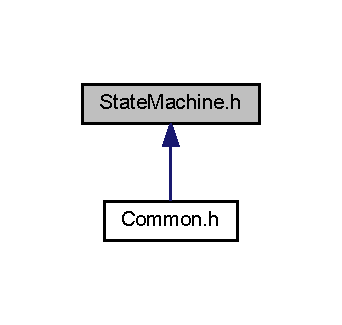
\includegraphics[width=164pt]{a00058}
\end{center}
\end{figure}
\subsection*{Functions}
\begin{DoxyCompactItemize}
\item 
void \hyperlink{a00038_a8c307b607d4931ec1214de3592c93df4}{sm\-Init} (void)
\end{DoxyCompactItemize}
\subsection*{Variables}
\begin{DoxyCompactItemize}
\item 
void($\ast$ \hyperlink{a00038_af1d16f7a57d6ced065765dcbb355fcde}{Alpha\-\_\-\-State\-\_\-\-Ptr} )(void)
\end{DoxyCompactItemize}


\subsection{Detailed Description}
State machine functions. 

\subsection{Function Documentation}
\hypertarget{a00038_a8c307b607d4931ec1214de3592c93df4}{\index{State\-Machine.\-h@{State\-Machine.\-h}!sm\-Init@{sm\-Init}}
\index{sm\-Init@{sm\-Init}!StateMachine.h@{State\-Machine.\-h}}
\subsubsection[{sm\-Init}]{\setlength{\rightskip}{0pt plus 5cm}void sm\-Init (
\begin{DoxyParamCaption}
\item[{void}]{}
\end{DoxyParamCaption}
)}}\label{a00038_a8c307b607d4931ec1214de3592c93df4}
Sets up the state machine (incl. timers) ready for use. 

\subsection{Variable Documentation}
\hypertarget{a00038_af1d16f7a57d6ced065765dcbb355fcde}{\index{State\-Machine.\-h@{State\-Machine.\-h}!Alpha\-\_\-\-State\-\_\-\-Ptr@{Alpha\-\_\-\-State\-\_\-\-Ptr}}
\index{Alpha\-\_\-\-State\-\_\-\-Ptr@{Alpha\-\_\-\-State\-\_\-\-Ptr}!StateMachine.h@{State\-Machine.\-h}}
\subsubsection[{Alpha\-\_\-\-State\-\_\-\-Ptr}]{\setlength{\rightskip}{0pt plus 5cm}void($\ast$ Alpha\-\_\-\-State\-\_\-\-Ptr)(void)}}\label{a00038_af1d16f7a57d6ced065765dcbb355fcde}
Runs the next iteration of the state machine. Should be called from the main super-\/loop. 
\hypertarget{a00040}{\section{Sci.\-h File Reference}
\label{a00040}\index{Sci.\-h@{Sci.\-h}}
}


Serial communications interface functions.  


This graph shows which files directly or indirectly include this file\-:\nopagebreak
\begin{figure}[H]
\begin{center}
\leavevmode
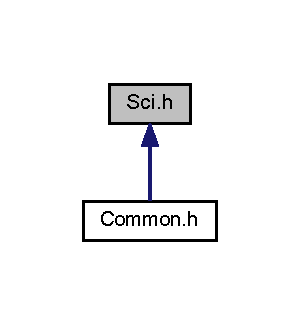
\includegraphics[width=144pt]{a00072}
\end{center}
\end{figure}
\subsection*{Macros}
\begin{DoxyCompactItemize}
\item 
\#define \hyperlink{a00040_a0e4c420431b12616b61e9f3a28f07e4d}{S\-C\-I\-B\-A\-U\-D\-\_\-\-M\-I\-N}~29
\item 
\#define \hyperlink{a00040_a5733933fffc18dbcb8bc9404e80bc493}{S\-C\-I\-F\-F\-R\-X\-\_\-\-I\-N\-T\-\_\-\-L\-V\-L}~1
\item 
\#define \hyperlink{a00040_a5340c9de55b8e5c65ef801d2dcabffd7}{S\-C\-I\-F\-F\-T\-X\-\_\-\-I\-N\-T\-\_\-\-L\-V\-L}~0
\item 
\#define \hyperlink{a00040_af0368b1c16e194a32bf4ce09eb937930}{S\-C\-I\-F\-F\-T\-X\-\_\-\-F\-I\-L\-L\-\_\-\-L\-V\-L}~4
\end{DoxyCompactItemize}
\subsection*{Functions}
\begin{DoxyCompactItemize}
\item 
Uint16 \hyperlink{a00040_a1f05b9c5226c73b67c1d6c3bf7f80b52}{sci\-Init} (Uint32 baud)
\item 
void \hyperlink{a00040_a941bdbf3e64ac5f4492a7f7c5936b445}{sci\-Tx} (void)
\end{DoxyCompactItemize}


\subsection{Detailed Description}
Serial communications interface functions. \begin{DoxyParagraph}{}
On the T\-I C2000 Launch\-Pad X\-L\-: \begin{TabularC}{3}
\hline
\rowcolor{lightgray}\PBS\centering {\bf Function}&\PBS\centering {\bf G\-P\-I\-O }&\PBS\centering {\bf P\-C\-B Pin  }\\\cline{1-3}
\PBS\centering S\-C\-I\-\_\-\-R\-X &\PBS\centering G\-P\-I\-O28&\PBS\centering J1-\/3 \\\cline{1-3}
\PBS\centering S\-C\-I\-\_\-\-T\-X &\PBS\centering G\-P\-I\-O29&\PBS\centering J1-\/4 \\\cline{1-3}
\end{TabularC}

\end{DoxyParagraph}
\begin{DoxyWarning}{Warning}
On the T\-I C2000 Launch\-Pad X\-L the switch 4 (S4) should be in the O\-F\-F position to communicate with devices other than the on-\/board U\-S\-B controller. 
\end{DoxyWarning}


\subsection{Macro Definition Documentation}
\hypertarget{a00040_a0e4c420431b12616b61e9f3a28f07e4d}{\index{Sci.\-h@{Sci.\-h}!S\-C\-I\-B\-A\-U\-D\-\_\-\-M\-I\-N@{S\-C\-I\-B\-A\-U\-D\-\_\-\-M\-I\-N}}
\index{S\-C\-I\-B\-A\-U\-D\-\_\-\-M\-I\-N@{S\-C\-I\-B\-A\-U\-D\-\_\-\-M\-I\-N}!Sci.h@{Sci.\-h}}
\subsubsection[{S\-C\-I\-B\-A\-U\-D\-\_\-\-M\-I\-N}]{\setlength{\rightskip}{0pt plus 5cm}\#define S\-C\-I\-B\-A\-U\-D\-\_\-\-M\-I\-N~29}}\label{a00040_a0e4c420431b12616b61e9f3a28f07e4d}
Minimum allowable value of S\-C\-I Baud. \hypertarget{a00040_a5733933fffc18dbcb8bc9404e80bc493}{\index{Sci.\-h@{Sci.\-h}!S\-C\-I\-F\-F\-R\-X\-\_\-\-I\-N\-T\-\_\-\-L\-V\-L@{S\-C\-I\-F\-F\-R\-X\-\_\-\-I\-N\-T\-\_\-\-L\-V\-L}}
\index{S\-C\-I\-F\-F\-R\-X\-\_\-\-I\-N\-T\-\_\-\-L\-V\-L@{S\-C\-I\-F\-F\-R\-X\-\_\-\-I\-N\-T\-\_\-\-L\-V\-L}!Sci.h@{Sci.\-h}}
\subsubsection[{S\-C\-I\-F\-F\-R\-X\-\_\-\-I\-N\-T\-\_\-\-L\-V\-L}]{\setlength{\rightskip}{0pt plus 5cm}\#define S\-C\-I\-F\-F\-R\-X\-\_\-\-I\-N\-T\-\_\-\-L\-V\-L~1}}\label{a00040_a5733933fffc18dbcb8bc9404e80bc493}
Interrupt level for receiving F\-I\-F\-O. \hypertarget{a00040_af0368b1c16e194a32bf4ce09eb937930}{\index{Sci.\-h@{Sci.\-h}!S\-C\-I\-F\-F\-T\-X\-\_\-\-F\-I\-L\-L\-\_\-\-L\-V\-L@{S\-C\-I\-F\-F\-T\-X\-\_\-\-F\-I\-L\-L\-\_\-\-L\-V\-L}}
\index{S\-C\-I\-F\-F\-T\-X\-\_\-\-F\-I\-L\-L\-\_\-\-L\-V\-L@{S\-C\-I\-F\-F\-T\-X\-\_\-\-F\-I\-L\-L\-\_\-\-L\-V\-L}!Sci.h@{Sci.\-h}}
\subsubsection[{S\-C\-I\-F\-F\-T\-X\-\_\-\-F\-I\-L\-L\-\_\-\-L\-V\-L}]{\setlength{\rightskip}{0pt plus 5cm}\#define S\-C\-I\-F\-F\-T\-X\-\_\-\-F\-I\-L\-L\-\_\-\-L\-V\-L~4}}\label{a00040_af0368b1c16e194a32bf4ce09eb937930}
Fill level for transmission F\-I\-F\-O. \hypertarget{a00040_a5340c9de55b8e5c65ef801d2dcabffd7}{\index{Sci.\-h@{Sci.\-h}!S\-C\-I\-F\-F\-T\-X\-\_\-\-I\-N\-T\-\_\-\-L\-V\-L@{S\-C\-I\-F\-F\-T\-X\-\_\-\-I\-N\-T\-\_\-\-L\-V\-L}}
\index{S\-C\-I\-F\-F\-T\-X\-\_\-\-I\-N\-T\-\_\-\-L\-V\-L@{S\-C\-I\-F\-F\-T\-X\-\_\-\-I\-N\-T\-\_\-\-L\-V\-L}!Sci.h@{Sci.\-h}}
\subsubsection[{S\-C\-I\-F\-F\-T\-X\-\_\-\-I\-N\-T\-\_\-\-L\-V\-L}]{\setlength{\rightskip}{0pt plus 5cm}\#define S\-C\-I\-F\-F\-T\-X\-\_\-\-I\-N\-T\-\_\-\-L\-V\-L~0}}\label{a00040_a5340c9de55b8e5c65ef801d2dcabffd7}
Interrupt level for transmission F\-I\-F\-O. 

\subsection{Function Documentation}
\hypertarget{a00040_a1f05b9c5226c73b67c1d6c3bf7f80b52}{\index{Sci.\-h@{Sci.\-h}!sci\-Init@{sci\-Init}}
\index{sci\-Init@{sci\-Init}!Sci.h@{Sci.\-h}}
\subsubsection[{sci\-Init}]{\setlength{\rightskip}{0pt plus 5cm}Uint16 sci\-Init (
\begin{DoxyParamCaption}
\item[{Uint32}]{baud}
\end{DoxyParamCaption}
)}}\label{a00040_a1f05b9c5226c73b67c1d6c3bf7f80b52}
Initialises the S\-C\-I(\-A) peripheral and relevant interrupts. 
\begin{DoxyParams}[1]{Parameters}
\mbox{\tt in}  & {\em baud} & The baud rate that the S\-C\-I should use minimum value is set by S\-C\-I\-B\-A\-U\-D\-\_\-\-M\-I\-N. \\
\hline
\end{DoxyParams}
\begin{DoxyReturn}{Returns}
Error status.
\end{DoxyReturn}
\begin{DoxyWarning}{Warning}
This function will clear any values already in the S\-C\-I peripheral registers. 

This function M\-U\-S\-T be called before any other S\-C\-I function. 
\end{DoxyWarning}
\hypertarget{a00040_a941bdbf3e64ac5f4492a7f7c5936b445}{\index{Sci.\-h@{Sci.\-h}!sci\-Tx@{sci\-Tx}}
\index{sci\-Tx@{sci\-Tx}!Sci.h@{Sci.\-h}}
\subsubsection[{sci\-Tx}]{\setlength{\rightskip}{0pt plus 5cm}void sci\-Tx (
\begin{DoxyParamCaption}
\item[{void}]{}
\end{DoxyParamCaption}
)}}\label{a00040_a941bdbf3e64ac5f4492a7f7c5936b445}
Transmits whatever data is on the S\-C\-P\-I output queue if S\-C\-I has been selected as the external communications type. 
\hypertarget{a00042}{\section{Tmp.\-h File Reference}
\label{a00042}\index{Tmp.\-h@{Tmp.\-h}}
}


Temperature sensor functions.  


This graph shows which files directly or indirectly include this file\-:\nopagebreak
\begin{figure}[H]
\begin{center}
\leavevmode
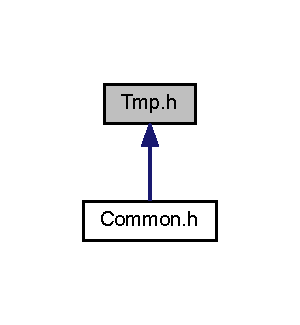
\includegraphics[width=144pt]{a00060}
\end{center}
\end{figure}
\subsection*{Macros}
\begin{DoxyCompactItemize}
\item 
\#define \hyperlink{a00042_a5fd3aabe18504a5314a5d0e71e3bc495}{A\-D\-C\-\_\-\-I2\-C\-\_\-\-A\-D\-D\-R}~0x48
\item 
\#define \hyperlink{a00042_a448e8a52be570dfe9fdddb2045039534}{A\-D\-C\-\_\-\-N\-U\-M\-\_\-\-C\-H\-N\-L}~0x08
\item 
\#define \hyperlink{a00042_a5a03d0b939a8dda552c9fe3319a82485}{A\-D\-C\-\_\-\-V\-R\-E\-F}~5.\-0
\item 
\#define \hyperlink{a00042_a9be6401f8c9339711816bec5ca55dd88}{A\-D\-C\-\_\-\-S\-T\-P\-S}~256
\item 
\#define \hyperlink{a00042_a6d41a70e126c748f2c99c3ff8228eb1b}{T\-M\-P\-\_\-\-V0\-C\-\_\-\-O\-F\-S\-T}~0.\-4
\item 
\#define \hyperlink{a00042_a0f910bb108922c8686a139977510af53}{T\-M\-P\-\_\-\-S\-C\-L\-\_\-\-O\-F\-S\-T}~\hyperlink{a00042_a6d41a70e126c748f2c99c3ff8228eb1b}{T\-M\-P\-\_\-\-V0\-C\-\_\-\-O\-F\-S\-T} $\ast$ \hyperlink{a00042_a9be6401f8c9339711816bec5ca55dd88}{A\-D\-C\-\_\-\-S\-T\-P\-S} / \hyperlink{a00042_a5a03d0b939a8dda552c9fe3319a82485}{A\-D\-C\-\_\-\-V\-R\-E\-F}
\item 
\#define \hyperlink{a00042_acc66f9f90ea4746679f5d26c834ddea5}{T\-M\-P\-\_\-\-E\-\_\-\-T\-\_\-\-C\-O\-L\-D}~1.\-5
\end{DoxyCompactItemize}
\subsection*{Functions}
\begin{DoxyCompactItemize}
\item 
Uint16 \hyperlink{a00042_a4f10186d5fb8a3069cc30c9d0c7e716f}{tmp\-Init} (void)
\item 
Uint16 \hyperlink{a00042_a10e85d2f2d7cce42822ea65e69601dfa}{tmp\-Set\-Otp} (Uint16 chnl, float32 tmp)
\item 
Uint16 \hyperlink{a00042_a9aedec904a421fed1823a16846b7841d}{tmp\-Get\-Otp} (Uint16 chnl, float32 $\ast$tmp\-Dest)
\item 
Uint16 \hyperlink{a00042_adf839085f18308f90ee198a96bbac364}{tmp\-Check\-Otp} (void)
\item 
Uint16 \hyperlink{a00042_a3f542f4bc433dfd2c1073a5e8308f99f}{tmp\-Read} (Uint16 chnl, float32 $\ast$tmp\-Dest)
\end{DoxyCompactItemize}


\subsection{Detailed Description}
Temperature sensor functions. The temperature sensor (M\-C\-P9701) output is read via an external A\-D\-C (A\-D\-S7830) that is connected to the I2\-C bus at address 10010xx where 'xx' is dependent upon the configuration of resistors R75 -\/ R78. All temperatures are in degrees Celcius.

\begin{DoxyWarning}{Warning}
Before any temperature functions can be used the I2\-C peripheral M\-U\-S\-T be initialised and \hyperlink{a00042_a4f10186d5fb8a3069cc30c9d0c7e716f}{tmp\-Init()} must be run -\/ \hyperlink{a00042_a4f10186d5fb8a3069cc30c9d0c7e716f}{tmp\-Init()} will require the interrupts to be enabled globally.
\end{DoxyWarning}
\begin{DoxySeeAlso}{See Also}
\hyperlink{a00019_a1e0a81a1ad1fd7710ca189236e3e5476}{i2c\-Init()} 
\end{DoxySeeAlso}


\subsection{Macro Definition Documentation}
\hypertarget{a00042_a5fd3aabe18504a5314a5d0e71e3bc495}{\index{Tmp.\-h@{Tmp.\-h}!A\-D\-C\-\_\-\-I2\-C\-\_\-\-A\-D\-D\-R@{A\-D\-C\-\_\-\-I2\-C\-\_\-\-A\-D\-D\-R}}
\index{A\-D\-C\-\_\-\-I2\-C\-\_\-\-A\-D\-D\-R@{A\-D\-C\-\_\-\-I2\-C\-\_\-\-A\-D\-D\-R}!Tmp.h@{Tmp.\-h}}
\subsubsection[{A\-D\-C\-\_\-\-I2\-C\-\_\-\-A\-D\-D\-R}]{\setlength{\rightskip}{0pt plus 5cm}\#define A\-D\-C\-\_\-\-I2\-C\-\_\-\-A\-D\-D\-R~0x48}}\label{a00042_a5fd3aabe18504a5314a5d0e71e3bc495}
Slave I2\-C address (A\-D\-S7830 8-\/channel A\-D\-C -\/ A0 = 0, A1 = 0). \hypertarget{a00042_a448e8a52be570dfe9fdddb2045039534}{\index{Tmp.\-h@{Tmp.\-h}!A\-D\-C\-\_\-\-N\-U\-M\-\_\-\-C\-H\-N\-L@{A\-D\-C\-\_\-\-N\-U\-M\-\_\-\-C\-H\-N\-L}}
\index{A\-D\-C\-\_\-\-N\-U\-M\-\_\-\-C\-H\-N\-L@{A\-D\-C\-\_\-\-N\-U\-M\-\_\-\-C\-H\-N\-L}!Tmp.h@{Tmp.\-h}}
\subsubsection[{A\-D\-C\-\_\-\-N\-U\-M\-\_\-\-C\-H\-N\-L}]{\setlength{\rightskip}{0pt plus 5cm}\#define A\-D\-C\-\_\-\-N\-U\-M\-\_\-\-C\-H\-N\-L~0x08}}\label{a00042_a448e8a52be570dfe9fdddb2045039534}
Number of temperature channels. The program expects a 50/50 split with first half for the on-\/board temperature channels. \hypertarget{a00042_a9be6401f8c9339711816bec5ca55dd88}{\index{Tmp.\-h@{Tmp.\-h}!A\-D\-C\-\_\-\-S\-T\-P\-S@{A\-D\-C\-\_\-\-S\-T\-P\-S}}
\index{A\-D\-C\-\_\-\-S\-T\-P\-S@{A\-D\-C\-\_\-\-S\-T\-P\-S}!Tmp.h@{Tmp.\-h}}
\subsubsection[{A\-D\-C\-\_\-\-S\-T\-P\-S}]{\setlength{\rightskip}{0pt plus 5cm}\#define A\-D\-C\-\_\-\-S\-T\-P\-S~256}}\label{a00042_a9be6401f8c9339711816bec5ca55dd88}
Number of A\-D\-S7830 A\-D\-C steps. \hypertarget{a00042_a5a03d0b939a8dda552c9fe3319a82485}{\index{Tmp.\-h@{Tmp.\-h}!A\-D\-C\-\_\-\-V\-R\-E\-F@{A\-D\-C\-\_\-\-V\-R\-E\-F}}
\index{A\-D\-C\-\_\-\-V\-R\-E\-F@{A\-D\-C\-\_\-\-V\-R\-E\-F}!Tmp.h@{Tmp.\-h}}
\subsubsection[{A\-D\-C\-\_\-\-V\-R\-E\-F}]{\setlength{\rightskip}{0pt plus 5cm}\#define A\-D\-C\-\_\-\-V\-R\-E\-F~5.\-0}}\label{a00042_a5a03d0b939a8dda552c9fe3319a82485}
A\-D\-S7830 A\-D\-C reference voltage (volts). \hypertarget{a00042_acc66f9f90ea4746679f5d26c834ddea5}{\index{Tmp.\-h@{Tmp.\-h}!T\-M\-P\-\_\-\-E\-\_\-\-T\-\_\-\-C\-O\-L\-D@{T\-M\-P\-\_\-\-E\-\_\-\-T\-\_\-\-C\-O\-L\-D}}
\index{T\-M\-P\-\_\-\-E\-\_\-\-T\-\_\-\-C\-O\-L\-D@{T\-M\-P\-\_\-\-E\-\_\-\-T\-\_\-\-C\-O\-L\-D}!Tmp.h@{Tmp.\-h}}
\subsubsection[{T\-M\-P\-\_\-\-E\-\_\-\-T\-\_\-\-C\-O\-L\-D}]{\setlength{\rightskip}{0pt plus 5cm}\#define T\-M\-P\-\_\-\-E\-\_\-\-T\-\_\-\-C\-O\-L\-D~1.\-5}}\label{a00042_acc66f9f90ea4746679f5d26c834ddea5}
M\-C\-P9701 Error at lowest operating temperature ( $ ^\circ$ C), calculated as shown in Microchip A\-N1001. \hypertarget{a00042_a0f910bb108922c8686a139977510af53}{\index{Tmp.\-h@{Tmp.\-h}!T\-M\-P\-\_\-\-S\-C\-L\-\_\-\-O\-F\-S\-T@{T\-M\-P\-\_\-\-S\-C\-L\-\_\-\-O\-F\-S\-T}}
\index{T\-M\-P\-\_\-\-S\-C\-L\-\_\-\-O\-F\-S\-T@{T\-M\-P\-\_\-\-S\-C\-L\-\_\-\-O\-F\-S\-T}!Tmp.h@{Tmp.\-h}}
\subsubsection[{T\-M\-P\-\_\-\-S\-C\-L\-\_\-\-O\-F\-S\-T}]{\setlength{\rightskip}{0pt plus 5cm}\#define T\-M\-P\-\_\-\-S\-C\-L\-\_\-\-O\-F\-S\-T~{\bf T\-M\-P\-\_\-\-V0\-C\-\_\-\-O\-F\-S\-T} $\ast$ {\bf A\-D\-C\-\_\-\-S\-T\-P\-S} / {\bf A\-D\-C\-\_\-\-V\-R\-E\-F}}}\label{a00042_a0f910bb108922c8686a139977510af53}
Scaled temperature offset. \hypertarget{a00042_a6d41a70e126c748f2c99c3ff8228eb1b}{\index{Tmp.\-h@{Tmp.\-h}!T\-M\-P\-\_\-\-V0\-C\-\_\-\-O\-F\-S\-T@{T\-M\-P\-\_\-\-V0\-C\-\_\-\-O\-F\-S\-T}}
\index{T\-M\-P\-\_\-\-V0\-C\-\_\-\-O\-F\-S\-T@{T\-M\-P\-\_\-\-V0\-C\-\_\-\-O\-F\-S\-T}!Tmp.h@{Tmp.\-h}}
\subsubsection[{T\-M\-P\-\_\-\-V0\-C\-\_\-\-O\-F\-S\-T}]{\setlength{\rightskip}{0pt plus 5cm}\#define T\-M\-P\-\_\-\-V0\-C\-\_\-\-O\-F\-S\-T~0.\-4}}\label{a00042_a6d41a70e126c748f2c99c3ff8228eb1b}
M\-C\-P9701 Temperature sensor $ V_{0{^\circ}C}$ (volts). 

\subsection{Function Documentation}
\hypertarget{a00042_adf839085f18308f90ee198a96bbac364}{\index{Tmp.\-h@{Tmp.\-h}!tmp\-Check\-Otp@{tmp\-Check\-Otp}}
\index{tmp\-Check\-Otp@{tmp\-Check\-Otp}!Tmp.h@{Tmp.\-h}}
\subsubsection[{tmp\-Check\-Otp}]{\setlength{\rightskip}{0pt plus 5cm}Uint16 tmp\-Check\-Otp (
\begin{DoxyParamCaption}
\item[{void}]{}
\end{DoxyParamCaption}
)}}\label{a00042_adf839085f18308f90ee198a96bbac364}
Tests the current on-\/board temperature sensor readings against the O\-T\-P limits. \begin{DoxyReturn}{Returns}
Error status. 
\end{DoxyReturn}
\hypertarget{a00042_a9aedec904a421fed1823a16846b7841d}{\index{Tmp.\-h@{Tmp.\-h}!tmp\-Get\-Otp@{tmp\-Get\-Otp}}
\index{tmp\-Get\-Otp@{tmp\-Get\-Otp}!Tmp.h@{Tmp.\-h}}
\subsubsection[{tmp\-Get\-Otp}]{\setlength{\rightskip}{0pt plus 5cm}Uint16 tmp\-Get\-Otp (
\begin{DoxyParamCaption}
\item[{Uint16}]{chnl, }
\item[{float32 $\ast$}]{tmp\-Dest}
\end{DoxyParamCaption}
)}}\label{a00042_a9aedec904a421fed1823a16846b7841d}
Queries the on-\/board over temperature limit for the specified channel. The I2\-C peripheral and temperature reading interface M\-U\-S\-T be initialised before this function is used. 
\begin{DoxyParams}[1]{Parameters}
\mbox{\tt in}  & {\em chnl} & Specifies the channel the setting is to be read from. \\
\hline
\mbox{\tt out}  & {\em tmp\-Dest} & Address of the memory location at which to place the query result ( $ ^\circ$ C). \\
\hline
\end{DoxyParams}
\begin{DoxyReturn}{Returns}
Error status. 
\end{DoxyReturn}
\hypertarget{a00042_a4f10186d5fb8a3069cc30c9d0c7e716f}{\index{Tmp.\-h@{Tmp.\-h}!tmp\-Init@{tmp\-Init}}
\index{tmp\-Init@{tmp\-Init}!Tmp.h@{Tmp.\-h}}
\subsubsection[{tmp\-Init}]{\setlength{\rightskip}{0pt plus 5cm}Uint16 tmp\-Init (
\begin{DoxyParamCaption}
\item[{void}]{}
\end{DoxyParamCaption}
)}}\label{a00042_a4f10186d5fb8a3069cc30c9d0c7e716f}
Initialises the system for temperature readings. The I2\-C peripheral must be initialised before this function is used \begin{DoxySeeAlso}{See Also}
\hyperlink{a00019_a1e0a81a1ad1fd7710ca189236e3e5476}{i2c\-Init()}. 
\end{DoxySeeAlso}
\begin{DoxyReturn}{Returns}
Error status. 
\end{DoxyReturn}
\hypertarget{a00042_a3f542f4bc433dfd2c1073a5e8308f99f}{\index{Tmp.\-h@{Tmp.\-h}!tmp\-Read@{tmp\-Read}}
\index{tmp\-Read@{tmp\-Read}!Tmp.h@{Tmp.\-h}}
\subsubsection[{tmp\-Read}]{\setlength{\rightskip}{0pt plus 5cm}Uint16 tmp\-Read (
\begin{DoxyParamCaption}
\item[{Uint16}]{chnl, }
\item[{float32 $\ast$}]{tmp\-Dest}
\end{DoxyParamCaption}
)}}\label{a00042_a3f542f4bc433dfd2c1073a5e8308f99f}
Queries the current on-\/board temperature of the specified channel. 
\begin{DoxyParams}[1]{Parameters}
\mbox{\tt in}  & {\em chnl} & Specifies the channel the temperature is to be read from. \\
\hline
\mbox{\tt out}  & {\em tmp\-Dest} & Address of the memory location at which to place the query result ( $ ^\circ$ C). \\
\hline
\end{DoxyParams}
\begin{DoxyReturn}{Returns}
Error status. 
\end{DoxyReturn}
\hypertarget{a00042_a10e85d2f2d7cce42822ea65e69601dfa}{\index{Tmp.\-h@{Tmp.\-h}!tmp\-Set\-Otp@{tmp\-Set\-Otp}}
\index{tmp\-Set\-Otp@{tmp\-Set\-Otp}!Tmp.h@{Tmp.\-h}}
\subsubsection[{tmp\-Set\-Otp}]{\setlength{\rightskip}{0pt plus 5cm}Uint16 tmp\-Set\-Otp (
\begin{DoxyParamCaption}
\item[{Uint16}]{chnl, }
\item[{float32}]{tmp}
\end{DoxyParamCaption}
)}}\label{a00042_a10e85d2f2d7cce42822ea65e69601dfa}
Sets the on-\/board over temperature limit for the specified channel. The I2\-C peripheral and temperature reading interface M\-U\-S\-T be initialised before this function is used. 
\begin{DoxyParams}[1]{Parameters}
\mbox{\tt in}  & {\em chnl} & Specifies the channel the setting is to be applied to. \\
\hline
\mbox{\tt in}  & {\em tmp} & Specifies the value of the limit to be applied ( $ ^\circ$ C). \\
\hline
\end{DoxyParams}
\begin{DoxyReturn}{Returns}
Error status. 
\end{DoxyReturn}

\hypertarget{a00043}{\section{Settings.\-h File Reference}
\label{a00043}\index{Settings.\-h@{Settings.\-h}}
}


Major build definitions and settings for the project.  


This graph shows which files directly or indirectly include this file\-:\nopagebreak
\begin{figure}[H]
\begin{center}
\leavevmode
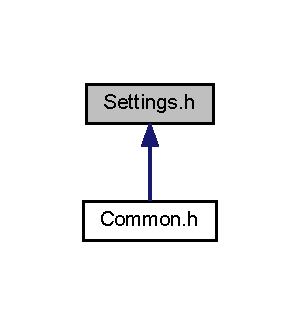
\includegraphics[width=144pt]{a00074}
\end{center}
\end{figure}
\subsection*{Macros}
\begin{DoxyCompactItemize}
\item 
\#define \hyperlink{a00043_abf493281a7e64fe88660c38753e18d56}{I\-N\-C\-R\-\_\-\-B\-U\-I\-L\-D}~2
\item 
\#define \hyperlink{a00043_ad72dbcf6d0153db1b8d8a58001feed83}{D\-E\-B\-U\-G}
\item 
\#define \hyperlink{a00043_a600b96e7a1d3cd28e228833bb61f8074}{D\-U\-A\-L\-\_\-\-C\-N\-T\-L\-\_\-\-A\-C}
\item 
\#define \hyperlink{a00043_a511faa1530ba984d340a884a97e6a80a}{V\-M\-I\-D\-\_\-\-R1}~540.\-0
\item 
\#define \hyperlink{a00043_a86d7f47e3c125143c21e1ca2836eb4ab}{V\-M\-I\-D\-\_\-\-R2}~4.\-3
\item 
\#define \hyperlink{a00043_a67fad1f78c49251e39fa6f1d5ff43e9e}{V\-A\-C\-\_\-\-R1}~540.\-0
\item 
\#define \hyperlink{a00043_a087778c4195e73f588e5c3cf7d9e9206}{V\-A\-C\-\_\-\-R2}~4.\-3
\item 
\#define \hyperlink{a00043_afe433b138bb71d8d26b6e0907e656d1b}{N\-U\-M\-\_\-\-C\-H\-N\-L\-S}~6
\item 
\#define \hyperlink{a00043_a1dd2b3b31e620e021371603376c6980f}{L\-O\-A\-D\-\_\-\-I\-D\-C\-L\-V\-L\-\_\-\-M\-A\-X}~35
\item 
\#define \hyperlink{a00043_ac460f1e706fdf51002f5dfc15c8eb5c9}{L\-O\-A\-D\-\_\-\-V\-D\-C\-L\-V\-L\-\_\-\-F\-I\-X}~60
\item 
\#define \hyperlink{a00043_aea1e2f7c212899b68d0cb6f4fcd1683d}{L\-O\-A\-D\-\_\-\-P\-W\-R\-L\-V\-L\-\_\-\-F\-I\-X}~200
\item 
\#define \hyperlink{a00043_ad873d002fba2a43978755cfb5e9ad5ee}{D\-C\-M\-I\-D\-\_\-\-V\-D\-C\-L\-V\-L\-\_\-\-F\-I\-X}~400
\item 
\#define \hyperlink{a00043_a2b577413184eb560f2f652b11deeba87}{A\-C\-\_\-\-I\-R\-M\-S\-L\-V\-L\-\_\-\-M\-A\-X}~10
\item 
\#define \hyperlink{a00043_afb09d50c3567117fe1f679ab1924d4ec}{A\-C\-\_\-\-V\-R\-M\-S\-L\-V\-L\-\_\-\-M\-A\-X}~250
\item 
\#define \hyperlink{a00043_aa5433ef3bc07259bf870e6e5e115c693}{A\-C\-\_\-\-P\-W\-R\-L\-V\-L\-\_\-\-F\-I\-X}~800
\item 
\#define \hyperlink{a00043_a39c57f59314d3cc076ca98898f227b46}{X\-F\-M\-R\-\_\-\-P\-W\-M\-F\-\_\-\-F\-I\-X}~130
\item 
\#define \hyperlink{a00043_abc63ab2a8e7782de38a5dbdfc33da717}{S\-Q\-R\-T\-\_\-2}~1.\-41429
\item 
\#define \hyperlink{a00043_ae468f418f2e6410dfcfeb58bcbbde516}{R\-E\-C\-P\-\_\-\-S\-Q\-R\-T\-\_\-2}~0.\-70711
\item 
\#define \hyperlink{a00043_a3c2e957a61cfa19e31e8477fe3aacab8}{V\-S\-S\-A}~0l
\item 
\#define \hyperlink{a00043_a2d52976aedaedf74a90019a689170620}{V\-D\-D\-A}~3300l
\item 
\#define \hyperlink{a00043_aa010c11f88da0f9a48a7dfd810412d5d}{u\-Sec100}~6000
\end{DoxyCompactItemize}
{\bf }\par
\begin{DoxyCompactItemize}
\item 
\#define \hyperlink{a00043_a5f4c019658ca5a8eff4bfc3d96d489a0}{C\-H\-A\-N\-N\-E\-L\-\_\-\-O\-O\-B}~0x10
\item 
\#define \hyperlink{a00043_a055087c0064c322a05e443b47479bfe1}{V\-A\-L\-U\-E\-\_\-\-O\-O\-B}~0x11
\item 
\#define \hyperlink{a00043_a42d97deed6614a0b5b0aee655055b43a}{O\-C\-P\-\_\-\-T\-R\-I\-P}~0x12
\item 
\#define \hyperlink{a00043_ac330c784fd08c389f8649ac8e34d29e8}{O\-V\-P\-\_\-\-T\-R\-I\-P}~0x13
\item 
\#define \hyperlink{a00043_a7037d8fd93cf1a2ae591b639614c0338}{O\-P\-P\-\_\-\-T\-R\-I\-P}~0x14
\item 
\#define \hyperlink{a00043_a5815c03ac63c324e326a148e247f24a1}{O\-T\-P\-\_\-\-T\-R\-I\-P}~0x15
\item 
\#define \hyperlink{a00043_aec1cab1af7dceb601fa90842135a4f65}{I2\-C\-\_\-\-R\-E\-A\-D\-\_\-\-W\-R\-O\-N\-G\-\_\-\-M\-S\-G}~0x20
\item 
\#define \hyperlink{a00043_ac6997f1781d1d9047bd556dd5152795b}{I2\-C\-\_\-\-W\-R\-I\-T\-E\-\_\-\-W\-R\-O\-N\-G\-\_\-\-M\-S\-G}~0x21
\item 
\#define \hyperlink{a00043_af623f6210c2ce545f939ec061fc533b0}{I2\-C\-\_\-\-S\-T\-P\-\_\-\-N\-O\-T\-\_\-\-R\-E\-A\-D\-Y}~0x22
\item 
\#define \hyperlink{a00043_ad3082827214b064d5b8289acaeb9ad20}{I2\-C\-\_\-\-B\-U\-S\-\_\-\-B\-U\-S\-Y}~0x23
\item 
\#define \hyperlink{a00043_a8e605ae1b9fc359d203b90cb9f8a090e}{I2\-C\-\_\-\-I\-N\-V\-A\-L\-I\-D\-\_\-\-I\-S\-R\-C}~0x24
\end{DoxyCompactItemize}



\subsection{Detailed Description}
Major build definitions and settings for the project. \begin{DoxyWarning}{Warning}
This file is included and referenced by I\-S\-R.\-asm, main() and mn\-Connect\-Nets().

When changes are made to this file please use rebuild all. 
\end{DoxyWarning}


\subsection{Macro Definition Documentation}
\hypertarget{a00043_a2b577413184eb560f2f652b11deeba87}{\index{Settings.\-h@{Settings.\-h}!A\-C\-\_\-\-I\-R\-M\-S\-L\-V\-L\-\_\-\-M\-A\-X@{A\-C\-\_\-\-I\-R\-M\-S\-L\-V\-L\-\_\-\-M\-A\-X}}
\index{A\-C\-\_\-\-I\-R\-M\-S\-L\-V\-L\-\_\-\-M\-A\-X@{A\-C\-\_\-\-I\-R\-M\-S\-L\-V\-L\-\_\-\-M\-A\-X}!Settings.h@{Settings.\-h}}
\subsubsection[{A\-C\-\_\-\-I\-R\-M\-S\-L\-V\-L\-\_\-\-M\-A\-X}]{\setlength{\rightskip}{0pt plus 5cm}\#define A\-C\-\_\-\-I\-R\-M\-S\-L\-V\-L\-\_\-\-M\-A\-X~10}}\label{a00043_a2b577413184eb560f2f652b11deeba87}
The maximum allowable value, in amps (R\-M\-S), for the A\-C current level. \hypertarget{a00043_aa5433ef3bc07259bf870e6e5e115c693}{\index{Settings.\-h@{Settings.\-h}!A\-C\-\_\-\-P\-W\-R\-L\-V\-L\-\_\-\-F\-I\-X@{A\-C\-\_\-\-P\-W\-R\-L\-V\-L\-\_\-\-F\-I\-X}}
\index{A\-C\-\_\-\-P\-W\-R\-L\-V\-L\-\_\-\-F\-I\-X@{A\-C\-\_\-\-P\-W\-R\-L\-V\-L\-\_\-\-F\-I\-X}!Settings.h@{Settings.\-h}}
\subsubsection[{A\-C\-\_\-\-P\-W\-R\-L\-V\-L\-\_\-\-F\-I\-X}]{\setlength{\rightskip}{0pt plus 5cm}\#define A\-C\-\_\-\-P\-W\-R\-L\-V\-L\-\_\-\-F\-I\-X~800}}\label{a00043_aa5433ef3bc07259bf870e6e5e115c693}
The fixed value, in watts, for the A\-C O\-P\-P level. \hypertarget{a00043_afb09d50c3567117fe1f679ab1924d4ec}{\index{Settings.\-h@{Settings.\-h}!A\-C\-\_\-\-V\-R\-M\-S\-L\-V\-L\-\_\-\-M\-A\-X@{A\-C\-\_\-\-V\-R\-M\-S\-L\-V\-L\-\_\-\-M\-A\-X}}
\index{A\-C\-\_\-\-V\-R\-M\-S\-L\-V\-L\-\_\-\-M\-A\-X@{A\-C\-\_\-\-V\-R\-M\-S\-L\-V\-L\-\_\-\-M\-A\-X}!Settings.h@{Settings.\-h}}
\subsubsection[{A\-C\-\_\-\-V\-R\-M\-S\-L\-V\-L\-\_\-\-M\-A\-X}]{\setlength{\rightskip}{0pt plus 5cm}\#define A\-C\-\_\-\-V\-R\-M\-S\-L\-V\-L\-\_\-\-M\-A\-X~250}}\label{a00043_afb09d50c3567117fe1f679ab1924d4ec}
The maximum allowable value, in volts (R\-M\-S), for the A\-C voltage level. \hypertarget{a00043_a5f4c019658ca5a8eff4bfc3d96d489a0}{\index{Settings.\-h@{Settings.\-h}!C\-H\-A\-N\-N\-E\-L\-\_\-\-O\-O\-B@{C\-H\-A\-N\-N\-E\-L\-\_\-\-O\-O\-B}}
\index{C\-H\-A\-N\-N\-E\-L\-\_\-\-O\-O\-B@{C\-H\-A\-N\-N\-E\-L\-\_\-\-O\-O\-B}!Settings.h@{Settings.\-h}}
\subsubsection[{C\-H\-A\-N\-N\-E\-L\-\_\-\-O\-O\-B}]{\setlength{\rightskip}{0pt plus 5cm}\#define C\-H\-A\-N\-N\-E\-L\-\_\-\-O\-O\-B~0x10}}\label{a00043_a5f4c019658ca5a8eff4bfc3d96d489a0}
Channel out of bounds error code. \hypertarget{a00043_ad873d002fba2a43978755cfb5e9ad5ee}{\index{Settings.\-h@{Settings.\-h}!D\-C\-M\-I\-D\-\_\-\-V\-D\-C\-L\-V\-L\-\_\-\-F\-I\-X@{D\-C\-M\-I\-D\-\_\-\-V\-D\-C\-L\-V\-L\-\_\-\-F\-I\-X}}
\index{D\-C\-M\-I\-D\-\_\-\-V\-D\-C\-L\-V\-L\-\_\-\-F\-I\-X@{D\-C\-M\-I\-D\-\_\-\-V\-D\-C\-L\-V\-L\-\_\-\-F\-I\-X}!Settings.h@{Settings.\-h}}
\subsubsection[{D\-C\-M\-I\-D\-\_\-\-V\-D\-C\-L\-V\-L\-\_\-\-F\-I\-X}]{\setlength{\rightskip}{0pt plus 5cm}\#define D\-C\-M\-I\-D\-\_\-\-V\-D\-C\-L\-V\-L\-\_\-\-F\-I\-X~400}}\label{a00043_ad873d002fba2a43978755cfb5e9ad5ee}
The fixed maximum value, in volts, for the D\-C mid voltage level. \hypertarget{a00043_ad72dbcf6d0153db1b8d8a58001feed83}{\index{Settings.\-h@{Settings.\-h}!D\-E\-B\-U\-G@{D\-E\-B\-U\-G}}
\index{D\-E\-B\-U\-G@{D\-E\-B\-U\-G}!Settings.h@{Settings.\-h}}
\subsubsection[{D\-E\-B\-U\-G}]{\setlength{\rightskip}{0pt plus 5cm}\#define D\-E\-B\-U\-G}}\label{a00043_ad72dbcf6d0153db1b8d8a58001feed83}
Includes and makes functions and variables public that are used only for debugging purposes. \hypertarget{a00043_a600b96e7a1d3cd28e228833bb61f8074}{\index{Settings.\-h@{Settings.\-h}!D\-U\-A\-L\-\_\-\-C\-N\-T\-L\-\_\-\-A\-C@{D\-U\-A\-L\-\_\-\-C\-N\-T\-L\-\_\-\-A\-C}}
\index{D\-U\-A\-L\-\_\-\-C\-N\-T\-L\-\_\-\-A\-C@{D\-U\-A\-L\-\_\-\-C\-N\-T\-L\-\_\-\-A\-C}!Settings.h@{Settings.\-h}}
\subsubsection[{D\-U\-A\-L\-\_\-\-C\-N\-T\-L\-\_\-\-A\-C}]{\setlength{\rightskip}{0pt plus 5cm}\#define D\-U\-A\-L\-\_\-\-C\-N\-T\-L\-\_\-\-A\-C}}\label{a00043_a600b96e7a1d3cd28e228833bb61f8074}
Uses the dual C\-N\-T\-L A\-C control instead of single V\-Ctrl. Cannot be used if P\-I\-D is still in use. \hypertarget{a00043_ad3082827214b064d5b8289acaeb9ad20}{\index{Settings.\-h@{Settings.\-h}!I2\-C\-\_\-\-B\-U\-S\-\_\-\-B\-U\-S\-Y@{I2\-C\-\_\-\-B\-U\-S\-\_\-\-B\-U\-S\-Y}}
\index{I2\-C\-\_\-\-B\-U\-S\-\_\-\-B\-U\-S\-Y@{I2\-C\-\_\-\-B\-U\-S\-\_\-\-B\-U\-S\-Y}!Settings.h@{Settings.\-h}}
\subsubsection[{I2\-C\-\_\-\-B\-U\-S\-\_\-\-B\-U\-S\-Y}]{\setlength{\rightskip}{0pt plus 5cm}\#define I2\-C\-\_\-\-B\-U\-S\-\_\-\-B\-U\-S\-Y~0x23}}\label{a00043_ad3082827214b064d5b8289acaeb9ad20}
I2\-C bus already busy error code. \hypertarget{a00043_a8e605ae1b9fc359d203b90cb9f8a090e}{\index{Settings.\-h@{Settings.\-h}!I2\-C\-\_\-\-I\-N\-V\-A\-L\-I\-D\-\_\-\-I\-S\-R\-C@{I2\-C\-\_\-\-I\-N\-V\-A\-L\-I\-D\-\_\-\-I\-S\-R\-C}}
\index{I2\-C\-\_\-\-I\-N\-V\-A\-L\-I\-D\-\_\-\-I\-S\-R\-C@{I2\-C\-\_\-\-I\-N\-V\-A\-L\-I\-D\-\_\-\-I\-S\-R\-C}!Settings.h@{Settings.\-h}}
\subsubsection[{I2\-C\-\_\-\-I\-N\-V\-A\-L\-I\-D\-\_\-\-I\-S\-R\-C}]{\setlength{\rightskip}{0pt plus 5cm}\#define I2\-C\-\_\-\-I\-N\-V\-A\-L\-I\-D\-\_\-\-I\-S\-R\-C~0x24}}\label{a00043_a8e605ae1b9fc359d203b90cb9f8a090e}
Invalid I2\-C interrupt source error code. \hypertarget{a00043_aec1cab1af7dceb601fa90842135a4f65}{\index{Settings.\-h@{Settings.\-h}!I2\-C\-\_\-\-R\-E\-A\-D\-\_\-\-W\-R\-O\-N\-G\-\_\-\-M\-S\-G@{I2\-C\-\_\-\-R\-E\-A\-D\-\_\-\-W\-R\-O\-N\-G\-\_\-\-M\-S\-G}}
\index{I2\-C\-\_\-\-R\-E\-A\-D\-\_\-\-W\-R\-O\-N\-G\-\_\-\-M\-S\-G@{I2\-C\-\_\-\-R\-E\-A\-D\-\_\-\-W\-R\-O\-N\-G\-\_\-\-M\-S\-G}!Settings.h@{Settings.\-h}}
\subsubsection[{I2\-C\-\_\-\-R\-E\-A\-D\-\_\-\-W\-R\-O\-N\-G\-\_\-\-M\-S\-G}]{\setlength{\rightskip}{0pt plus 5cm}\#define I2\-C\-\_\-\-R\-E\-A\-D\-\_\-\-W\-R\-O\-N\-G\-\_\-\-M\-S\-G~0x20}}\label{a00043_aec1cab1af7dceb601fa90842135a4f65}
Incorrect type I2\-C message read error code. \hypertarget{a00043_af623f6210c2ce545f939ec061fc533b0}{\index{Settings.\-h@{Settings.\-h}!I2\-C\-\_\-\-S\-T\-P\-\_\-\-N\-O\-T\-\_\-\-R\-E\-A\-D\-Y@{I2\-C\-\_\-\-S\-T\-P\-\_\-\-N\-O\-T\-\_\-\-R\-E\-A\-D\-Y}}
\index{I2\-C\-\_\-\-S\-T\-P\-\_\-\-N\-O\-T\-\_\-\-R\-E\-A\-D\-Y@{I2\-C\-\_\-\-S\-T\-P\-\_\-\-N\-O\-T\-\_\-\-R\-E\-A\-D\-Y}!Settings.h@{Settings.\-h}}
\subsubsection[{I2\-C\-\_\-\-S\-T\-P\-\_\-\-N\-O\-T\-\_\-\-R\-E\-A\-D\-Y}]{\setlength{\rightskip}{0pt plus 5cm}\#define I2\-C\-\_\-\-S\-T\-P\-\_\-\-N\-O\-T\-\_\-\-R\-E\-A\-D\-Y~0x22}}\label{a00043_af623f6210c2ce545f939ec061fc533b0}
I2\-C stop bit was not yet received error code. \hypertarget{a00043_ac6997f1781d1d9047bd556dd5152795b}{\index{Settings.\-h@{Settings.\-h}!I2\-C\-\_\-\-W\-R\-I\-T\-E\-\_\-\-W\-R\-O\-N\-G\-\_\-\-M\-S\-G@{I2\-C\-\_\-\-W\-R\-I\-T\-E\-\_\-\-W\-R\-O\-N\-G\-\_\-\-M\-S\-G}}
\index{I2\-C\-\_\-\-W\-R\-I\-T\-E\-\_\-\-W\-R\-O\-N\-G\-\_\-\-M\-S\-G@{I2\-C\-\_\-\-W\-R\-I\-T\-E\-\_\-\-W\-R\-O\-N\-G\-\_\-\-M\-S\-G}!Settings.h@{Settings.\-h}}
\subsubsection[{I2\-C\-\_\-\-W\-R\-I\-T\-E\-\_\-\-W\-R\-O\-N\-G\-\_\-\-M\-S\-G}]{\setlength{\rightskip}{0pt plus 5cm}\#define I2\-C\-\_\-\-W\-R\-I\-T\-E\-\_\-\-W\-R\-O\-N\-G\-\_\-\-M\-S\-G~0x21}}\label{a00043_ac6997f1781d1d9047bd556dd5152795b}
Incorrect type I2\-C write message error code. \hypertarget{a00043_abf493281a7e64fe88660c38753e18d56}{\index{Settings.\-h@{Settings.\-h}!I\-N\-C\-R\-\_\-\-B\-U\-I\-L\-D@{I\-N\-C\-R\-\_\-\-B\-U\-I\-L\-D}}
\index{I\-N\-C\-R\-\_\-\-B\-U\-I\-L\-D@{I\-N\-C\-R\-\_\-\-B\-U\-I\-L\-D}!Settings.h@{Settings.\-h}}
\subsubsection[{I\-N\-C\-R\-\_\-\-B\-U\-I\-L\-D}]{\setlength{\rightskip}{0pt plus 5cm}\#define I\-N\-C\-R\-\_\-\-B\-U\-I\-L\-D~2}}\label{a00043_abf493281a7e64fe88660c38753e18d56}
Alters the digital power control loop between closed or open. Open-\/\-Loop\-: 1. Closed-\/loop\-: 2. \hypertarget{a00043_a1dd2b3b31e620e021371603376c6980f}{\index{Settings.\-h@{Settings.\-h}!L\-O\-A\-D\-\_\-\-I\-D\-C\-L\-V\-L\-\_\-\-M\-A\-X@{L\-O\-A\-D\-\_\-\-I\-D\-C\-L\-V\-L\-\_\-\-M\-A\-X}}
\index{L\-O\-A\-D\-\_\-\-I\-D\-C\-L\-V\-L\-\_\-\-M\-A\-X@{L\-O\-A\-D\-\_\-\-I\-D\-C\-L\-V\-L\-\_\-\-M\-A\-X}!Settings.h@{Settings.\-h}}
\subsubsection[{L\-O\-A\-D\-\_\-\-I\-D\-C\-L\-V\-L\-\_\-\-M\-A\-X}]{\setlength{\rightskip}{0pt plus 5cm}\#define L\-O\-A\-D\-\_\-\-I\-D\-C\-L\-V\-L\-\_\-\-M\-A\-X~35}}\label{a00043_a1dd2b3b31e620e021371603376c6980f}
The maximum allowable value, in amps, for the load current levels. \hypertarget{a00043_aea1e2f7c212899b68d0cb6f4fcd1683d}{\index{Settings.\-h@{Settings.\-h}!L\-O\-A\-D\-\_\-\-P\-W\-R\-L\-V\-L\-\_\-\-F\-I\-X@{L\-O\-A\-D\-\_\-\-P\-W\-R\-L\-V\-L\-\_\-\-F\-I\-X}}
\index{L\-O\-A\-D\-\_\-\-P\-W\-R\-L\-V\-L\-\_\-\-F\-I\-X@{L\-O\-A\-D\-\_\-\-P\-W\-R\-L\-V\-L\-\_\-\-F\-I\-X}!Settings.h@{Settings.\-h}}
\subsubsection[{L\-O\-A\-D\-\_\-\-P\-W\-R\-L\-V\-L\-\_\-\-F\-I\-X}]{\setlength{\rightskip}{0pt plus 5cm}\#define L\-O\-A\-D\-\_\-\-P\-W\-R\-L\-V\-L\-\_\-\-F\-I\-X~200}}\label{a00043_aea1e2f7c212899b68d0cb6f4fcd1683d}
The fixed maximum value, in watts, for the load power levels. \hypertarget{a00043_ac460f1e706fdf51002f5dfc15c8eb5c9}{\index{Settings.\-h@{Settings.\-h}!L\-O\-A\-D\-\_\-\-V\-D\-C\-L\-V\-L\-\_\-\-F\-I\-X@{L\-O\-A\-D\-\_\-\-V\-D\-C\-L\-V\-L\-\_\-\-F\-I\-X}}
\index{L\-O\-A\-D\-\_\-\-V\-D\-C\-L\-V\-L\-\_\-\-F\-I\-X@{L\-O\-A\-D\-\_\-\-V\-D\-C\-L\-V\-L\-\_\-\-F\-I\-X}!Settings.h@{Settings.\-h}}
\subsubsection[{L\-O\-A\-D\-\_\-\-V\-D\-C\-L\-V\-L\-\_\-\-F\-I\-X}]{\setlength{\rightskip}{0pt plus 5cm}\#define L\-O\-A\-D\-\_\-\-V\-D\-C\-L\-V\-L\-\_\-\-F\-I\-X~60}}\label{a00043_ac460f1e706fdf51002f5dfc15c8eb5c9}
The fixed maximum value, in volts, for the load voltage levels. \hypertarget{a00043_afe433b138bb71d8d26b6e0907e656d1b}{\index{Settings.\-h@{Settings.\-h}!N\-U\-M\-\_\-\-C\-H\-N\-L\-S@{N\-U\-M\-\_\-\-C\-H\-N\-L\-S}}
\index{N\-U\-M\-\_\-\-C\-H\-N\-L\-S@{N\-U\-M\-\_\-\-C\-H\-N\-L\-S}!Settings.h@{Settings.\-h}}
\subsubsection[{N\-U\-M\-\_\-\-C\-H\-N\-L\-S}]{\setlength{\rightskip}{0pt plus 5cm}\#define N\-U\-M\-\_\-\-C\-H\-N\-L\-S~6}}\label{a00043_afe433b138bb71d8d26b6e0907e656d1b}
Total number of I\-I\-R filter control law macros used (doesn't include V\-M\-I\-D semi-\/channel). \hypertarget{a00043_a42d97deed6614a0b5b0aee655055b43a}{\index{Settings.\-h@{Settings.\-h}!O\-C\-P\-\_\-\-T\-R\-I\-P@{O\-C\-P\-\_\-\-T\-R\-I\-P}}
\index{O\-C\-P\-\_\-\-T\-R\-I\-P@{O\-C\-P\-\_\-\-T\-R\-I\-P}!Settings.h@{Settings.\-h}}
\subsubsection[{O\-C\-P\-\_\-\-T\-R\-I\-P}]{\setlength{\rightskip}{0pt plus 5cm}\#define O\-C\-P\-\_\-\-T\-R\-I\-P~0x12}}\label{a00043_a42d97deed6614a0b5b0aee655055b43a}
Over-\/current protection trip error code. \hypertarget{a00043_a7037d8fd93cf1a2ae591b639614c0338}{\index{Settings.\-h@{Settings.\-h}!O\-P\-P\-\_\-\-T\-R\-I\-P@{O\-P\-P\-\_\-\-T\-R\-I\-P}}
\index{O\-P\-P\-\_\-\-T\-R\-I\-P@{O\-P\-P\-\_\-\-T\-R\-I\-P}!Settings.h@{Settings.\-h}}
\subsubsection[{O\-P\-P\-\_\-\-T\-R\-I\-P}]{\setlength{\rightskip}{0pt plus 5cm}\#define O\-P\-P\-\_\-\-T\-R\-I\-P~0x14}}\label{a00043_a7037d8fd93cf1a2ae591b639614c0338}
Over-\/power protection trip error code. \hypertarget{a00043_a5815c03ac63c324e326a148e247f24a1}{\index{Settings.\-h@{Settings.\-h}!O\-T\-P\-\_\-\-T\-R\-I\-P@{O\-T\-P\-\_\-\-T\-R\-I\-P}}
\index{O\-T\-P\-\_\-\-T\-R\-I\-P@{O\-T\-P\-\_\-\-T\-R\-I\-P}!Settings.h@{Settings.\-h}}
\subsubsection[{O\-T\-P\-\_\-\-T\-R\-I\-P}]{\setlength{\rightskip}{0pt plus 5cm}\#define O\-T\-P\-\_\-\-T\-R\-I\-P~0x15}}\label{a00043_a5815c03ac63c324e326a148e247f24a1}
Over-\/temperature protection trip error code. \hypertarget{a00043_ac330c784fd08c389f8649ac8e34d29e8}{\index{Settings.\-h@{Settings.\-h}!O\-V\-P\-\_\-\-T\-R\-I\-P@{O\-V\-P\-\_\-\-T\-R\-I\-P}}
\index{O\-V\-P\-\_\-\-T\-R\-I\-P@{O\-V\-P\-\_\-\-T\-R\-I\-P}!Settings.h@{Settings.\-h}}
\subsubsection[{O\-V\-P\-\_\-\-T\-R\-I\-P}]{\setlength{\rightskip}{0pt plus 5cm}\#define O\-V\-P\-\_\-\-T\-R\-I\-P~0x13}}\label{a00043_ac330c784fd08c389f8649ac8e34d29e8}
Over-\/voltage protection trip error code. \hypertarget{a00043_ae468f418f2e6410dfcfeb58bcbbde516}{\index{Settings.\-h@{Settings.\-h}!R\-E\-C\-P\-\_\-\-S\-Q\-R\-T\-\_\-2@{R\-E\-C\-P\-\_\-\-S\-Q\-R\-T\-\_\-2}}
\index{R\-E\-C\-P\-\_\-\-S\-Q\-R\-T\-\_\-2@{R\-E\-C\-P\-\_\-\-S\-Q\-R\-T\-\_\-2}!Settings.h@{Settings.\-h}}
\subsubsection[{R\-E\-C\-P\-\_\-\-S\-Q\-R\-T\-\_\-2}]{\setlength{\rightskip}{0pt plus 5cm}\#define R\-E\-C\-P\-\_\-\-S\-Q\-R\-T\-\_\-2~0.\-70711}}\label{a00043_ae468f418f2e6410dfcfeb58bcbbde516}
1/sqrt(2) constant used for R\-M\-S calculations. \hypertarget{a00043_abc63ab2a8e7782de38a5dbdfc33da717}{\index{Settings.\-h@{Settings.\-h}!S\-Q\-R\-T\-\_\-2@{S\-Q\-R\-T\-\_\-2}}
\index{S\-Q\-R\-T\-\_\-2@{S\-Q\-R\-T\-\_\-2}!Settings.h@{Settings.\-h}}
\subsubsection[{S\-Q\-R\-T\-\_\-2}]{\setlength{\rightskip}{0pt plus 5cm}\#define S\-Q\-R\-T\-\_\-2~1.\-41429}}\label{a00043_abc63ab2a8e7782de38a5dbdfc33da717}
Sqrt(2) constant used for R\-M\-S calculations. \hypertarget{a00043_aa010c11f88da0f9a48a7dfd810412d5d}{\index{Settings.\-h@{Settings.\-h}!u\-Sec100@{u\-Sec100}}
\index{u\-Sec100@{u\-Sec100}!Settings.h@{Settings.\-h}}
\subsubsection[{u\-Sec100}]{\setlength{\rightskip}{0pt plus 5cm}\#define u\-Sec100~6000}}\label{a00043_aa010c11f88da0f9a48a7dfd810412d5d}
100us -\/ System define. \hypertarget{a00043_a67fad1f78c49251e39fa6f1d5ff43e9e}{\index{Settings.\-h@{Settings.\-h}!V\-A\-C\-\_\-\-R1@{V\-A\-C\-\_\-\-R1}}
\index{V\-A\-C\-\_\-\-R1@{V\-A\-C\-\_\-\-R1}!Settings.h@{Settings.\-h}}
\subsubsection[{V\-A\-C\-\_\-\-R1}]{\setlength{\rightskip}{0pt plus 5cm}\#define V\-A\-C\-\_\-\-R1~540.\-0}}\label{a00043_a67fad1f78c49251e39fa6f1d5ff43e9e}
Scaling voltage divider R1 resistor value for V\-A\-C A\-D\-C. \hypertarget{a00043_a087778c4195e73f588e5c3cf7d9e9206}{\index{Settings.\-h@{Settings.\-h}!V\-A\-C\-\_\-\-R2@{V\-A\-C\-\_\-\-R2}}
\index{V\-A\-C\-\_\-\-R2@{V\-A\-C\-\_\-\-R2}!Settings.h@{Settings.\-h}}
\subsubsection[{V\-A\-C\-\_\-\-R2}]{\setlength{\rightskip}{0pt plus 5cm}\#define V\-A\-C\-\_\-\-R2~4.\-3}}\label{a00043_a087778c4195e73f588e5c3cf7d9e9206}
Scaling voltage divider R2 resistor value for V\-A\-C A\-D\-C. \hypertarget{a00043_a055087c0064c322a05e443b47479bfe1}{\index{Settings.\-h@{Settings.\-h}!V\-A\-L\-U\-E\-\_\-\-O\-O\-B@{V\-A\-L\-U\-E\-\_\-\-O\-O\-B}}
\index{V\-A\-L\-U\-E\-\_\-\-O\-O\-B@{V\-A\-L\-U\-E\-\_\-\-O\-O\-B}!Settings.h@{Settings.\-h}}
\subsubsection[{V\-A\-L\-U\-E\-\_\-\-O\-O\-B}]{\setlength{\rightskip}{0pt plus 5cm}\#define V\-A\-L\-U\-E\-\_\-\-O\-O\-B~0x11}}\label{a00043_a055087c0064c322a05e443b47479bfe1}
Value out of bounds error code. \hypertarget{a00043_a2d52976aedaedf74a90019a689170620}{\index{Settings.\-h@{Settings.\-h}!V\-D\-D\-A@{V\-D\-D\-A}}
\index{V\-D\-D\-A@{V\-D\-D\-A}!Settings.h@{Settings.\-h}}
\subsubsection[{V\-D\-D\-A}]{\setlength{\rightskip}{0pt plus 5cm}\#define V\-D\-D\-A~3300l}}\label{a00043_a2d52976aedaedf74a90019a689170620}
System V\-M\-A\-X\-R\-E\-F (millivolts). \hypertarget{a00043_a511faa1530ba984d340a884a97e6a80a}{\index{Settings.\-h@{Settings.\-h}!V\-M\-I\-D\-\_\-\-R1@{V\-M\-I\-D\-\_\-\-R1}}
\index{V\-M\-I\-D\-\_\-\-R1@{V\-M\-I\-D\-\_\-\-R1}!Settings.h@{Settings.\-h}}
\subsubsection[{V\-M\-I\-D\-\_\-\-R1}]{\setlength{\rightskip}{0pt plus 5cm}\#define V\-M\-I\-D\-\_\-\-R1~540.\-0}}\label{a00043_a511faa1530ba984d340a884a97e6a80a}
Scaling voltage divider R1 resistor value for V\-M\-I\-D A\-D\-C. \hypertarget{a00043_a86d7f47e3c125143c21e1ca2836eb4ab}{\index{Settings.\-h@{Settings.\-h}!V\-M\-I\-D\-\_\-\-R2@{V\-M\-I\-D\-\_\-\-R2}}
\index{V\-M\-I\-D\-\_\-\-R2@{V\-M\-I\-D\-\_\-\-R2}!Settings.h@{Settings.\-h}}
\subsubsection[{V\-M\-I\-D\-\_\-\-R2}]{\setlength{\rightskip}{0pt plus 5cm}\#define V\-M\-I\-D\-\_\-\-R2~4.\-3}}\label{a00043_a86d7f47e3c125143c21e1ca2836eb4ab}
Scaling voltage divider R2 resistor value for V\-M\-I\-D A\-D\-C. \hypertarget{a00043_a3c2e957a61cfa19e31e8477fe3aacab8}{\index{Settings.\-h@{Settings.\-h}!V\-S\-S\-A@{V\-S\-S\-A}}
\index{V\-S\-S\-A@{V\-S\-S\-A}!Settings.h@{Settings.\-h}}
\subsubsection[{V\-S\-S\-A}]{\setlength{\rightskip}{0pt plus 5cm}\#define V\-S\-S\-A~0l}}\label{a00043_a3c2e957a61cfa19e31e8477fe3aacab8}
System V\-L\-O\-W\-R\-E\-F (millivolts). \hypertarget{a00043_a39c57f59314d3cc076ca98898f227b46}{\index{Settings.\-h@{Settings.\-h}!X\-F\-M\-R\-\_\-\-P\-W\-M\-F\-\_\-\-F\-I\-X@{X\-F\-M\-R\-\_\-\-P\-W\-M\-F\-\_\-\-F\-I\-X}}
\index{X\-F\-M\-R\-\_\-\-P\-W\-M\-F\-\_\-\-F\-I\-X@{X\-F\-M\-R\-\_\-\-P\-W\-M\-F\-\_\-\-F\-I\-X}!Settings.h@{Settings.\-h}}
\subsubsection[{X\-F\-M\-R\-\_\-\-P\-W\-M\-F\-\_\-\-F\-I\-X}]{\setlength{\rightskip}{0pt plus 5cm}\#define X\-F\-M\-R\-\_\-\-P\-W\-M\-F\-\_\-\-F\-I\-X~130}}\label{a00043_a39c57f59314d3cc076ca98898f227b46}
The fixed frequency (k\-Hz) setting for the transformer P\-W\-M (at 50\% duty). 
\hypertarget{a00045}{\section{Sine\-Gen.\-h File Reference}
\label{a00045}\index{Sine\-Gen.\-h@{Sine\-Gen.\-h}}
}


Signal generator functions.  


This graph shows which files directly or indirectly include this file\-:\nopagebreak
\begin{figure}[H]
\begin{center}
\leavevmode
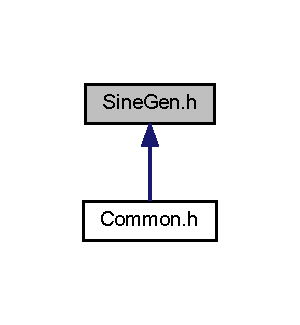
\includegraphics[width=144pt]{a00075}
\end{center}
\end{figure}
\subsection*{Macros}
\begin{DoxyCompactItemize}
\item 
\#define \hyperlink{a00045_af54d156f326804e0c3d80e0b709d3406}{S\-I\-N\-\_\-\-F\-\_\-\-I\-S\-R}~60000000.\-0f/\-P\-W\-M\-\_\-1\-\_\-\-P\-R\-D
\item 
\#define \hyperlink{a00045_ae3860ce29591dbf34c90a5cdce35ad86}{S\-I\-N\-\_\-\-F\-\_\-\-I\-S\-R\-\_\-\-D\-V\-S\-R}~6
\item 
\#define \hyperlink{a00045_a67755e274de5a3185ae6ce437a5f6e7d}{S\-I\-N\-\_\-\-F\-\_\-\-M\-A\-X}~200u
\item 
\#define \hyperlink{a00045_a58bd24055692a8794616ff2bc5c84d51}{S\-I\-N\-\_\-\-F\-\_\-\-R\-E\-Q}~50.\-0
\item 
\#define \hyperlink{a00045_a992c375a2083a58aa46c0600fea7df64}{S\-I\-N\-\_\-\-O\-F\-S\-T}~0
\item 
\#define \hyperlink{a00045_abd714e85d6aa6a48b8d84a41b43074c2}{S\-I\-N\-\_\-\-P\-H\-S\-E}~0
\item 
\#define \hyperlink{a00045_aa63a6918009b4e4381e359cee2f05eef}{S\-I\-N\-\_\-\-D\-F\-L\-T\-\_\-\-G\-A\-I\-N}~0.\-0
\item 
\#define \hyperlink{a00045_afc105af9d8f851266d0b8e8ffe57931a}{S\-I\-N\-\_\-\-D\-F\-L\-T\-\_\-\-R\-C\-T\-F\-Y}~T\-R\-U\-E
\item 
\#define \hyperlink{a00045_a71b6211a4d077af219d7e503f17114d1}{S\-I\-N\-\_\-\-C\-H\-A\-N\-N\-E\-L}~\hyperlink{a00027_a3fc4318ae73eae35339f616047300b0f}{A\-C\-\_\-\-S\-T\-A\-G\-E}
\end{DoxyCompactItemize}
\subsection*{Functions}
\begin{DoxyCompactItemize}
\item 
void \hyperlink{a00045_a4c050cf5f44fdac62f2260da4d5d6c32}{init\-Sine} (Uint16 enable\-Phase\-Out)
\item 
void \hyperlink{a00045_a5cd2ce3a0a44bf15cce989d0ec28483c}{update\-Sine\-Gain} (void)
\item 
void \hyperlink{a00045_a15cc3f7f606ea48016c591c798a55f15}{update\-Sine\-Signal} (void)
\item 
void \hyperlink{a00045_ab3922b82823a89211338cee98117369c}{enable\-Sine\-Phase\-Out} (void)
\item 
void \hyperlink{a00045_af1add0fec8d10afcd40956d01d01cfa7}{disable\-Sine\-Phase\-Out} (void)
\item 
Uint16 \hyperlink{a00045_a70155ca3a5315917719d943e645e53d6}{set\-Sine\-State} (Uint16 state)
\item 
Uint16 \hyperlink{a00045_a63e4f7727c81ef635e50879433bc03b9}{get\-Sine\-State} (Uint16 $\ast$state)
\item 
Uint16 \hyperlink{a00045_a2604c70758904f640d943151c13ddb9b}{set\-Sine\-Rms\-Target} (float32 rms\-Target)
\item 
Uint16 \hyperlink{a00045_ab40939821b2aba026ef55cf4ec9c12dd}{set\-Sine\-Gain\-Target} (float32 target)
\item 
Uint16 \hyperlink{a00045_a713b866aa5b5636f85d1a1f5f06b4ed3}{get\-Sine\-Gain\-Target} (float32 $\ast$target)
\item 
Uint16 \hyperlink{a00045_ae25f691d4da06e89110ade79a0a4d93b}{set\-Sine\-Gain\-Step} (float32 step)
\item 
Uint16 \hyperlink{a00045_a5ab11b6c0a463f9791e61647c89f5ebe}{get\-Sine\-Gain\-Step} (float32 $\ast$step)
\end{DoxyCompactItemize}
\subsection*{Variables}
\begin{DoxyCompactItemize}
\item 
volatile int32 $\ast$ \hyperlink{a00045_a5dba1fe543c9e62ef6cc8cf4179de951}{S\-G\-E\-N\-T\-I\-\_\-1ch\-\_\-\-V\-Out}
\end{DoxyCompactItemize}


\subsection{Detailed Description}
Signal generator functions. sg\-Init() must be called before any other signal generator functions are used. Note that the frequency resolution is determined by the maximum frequency and the step max. For further details, see the signal generator library documentation (Texas Instruments Signal Generator Library Module user's Guide).

\begin{DoxyWarning}{Warning}
This file is included by the file I\-S\-R.\-asm. 
\end{DoxyWarning}


\subsection{Macro Definition Documentation}
\hypertarget{a00045_a71b6211a4d077af219d7e503f17114d1}{\index{Sine\-Gen.\-h@{Sine\-Gen.\-h}!S\-I\-N\-\_\-\-C\-H\-A\-N\-N\-E\-L@{S\-I\-N\-\_\-\-C\-H\-A\-N\-N\-E\-L}}
\index{S\-I\-N\-\_\-\-C\-H\-A\-N\-N\-E\-L@{S\-I\-N\-\_\-\-C\-H\-A\-N\-N\-E\-L}!SineGen.h@{Sine\-Gen.\-h}}
\subsubsection[{S\-I\-N\-\_\-\-C\-H\-A\-N\-N\-E\-L}]{\setlength{\rightskip}{0pt plus 5cm}\#define S\-I\-N\-\_\-\-C\-H\-A\-N\-N\-E\-L~{\bf A\-C\-\_\-\-S\-T\-A\-G\-E}}}\label{a00045_a71b6211a4d077af219d7e503f17114d1}
Defines which channel enable controls the generator output. \hypertarget{a00045_aa63a6918009b4e4381e359cee2f05eef}{\index{Sine\-Gen.\-h@{Sine\-Gen.\-h}!S\-I\-N\-\_\-\-D\-F\-L\-T\-\_\-\-G\-A\-I\-N@{S\-I\-N\-\_\-\-D\-F\-L\-T\-\_\-\-G\-A\-I\-N}}
\index{S\-I\-N\-\_\-\-D\-F\-L\-T\-\_\-\-G\-A\-I\-N@{S\-I\-N\-\_\-\-D\-F\-L\-T\-\_\-\-G\-A\-I\-N}!SineGen.h@{Sine\-Gen.\-h}}
\subsubsection[{S\-I\-N\-\_\-\-D\-F\-L\-T\-\_\-\-G\-A\-I\-N}]{\setlength{\rightskip}{0pt plus 5cm}\#define S\-I\-N\-\_\-\-D\-F\-L\-T\-\_\-\-G\-A\-I\-N~0.\-0}}\label{a00045_aa63a6918009b4e4381e359cee2f05eef}
Initial gain setting \mbox{[}0.\-0, 1.\-0\mbox{]}. \hypertarget{a00045_afc105af9d8f851266d0b8e8ffe57931a}{\index{Sine\-Gen.\-h@{Sine\-Gen.\-h}!S\-I\-N\-\_\-\-D\-F\-L\-T\-\_\-\-R\-C\-T\-F\-Y@{S\-I\-N\-\_\-\-D\-F\-L\-T\-\_\-\-R\-C\-T\-F\-Y}}
\index{S\-I\-N\-\_\-\-D\-F\-L\-T\-\_\-\-R\-C\-T\-F\-Y@{S\-I\-N\-\_\-\-D\-F\-L\-T\-\_\-\-R\-C\-T\-F\-Y}!SineGen.h@{Sine\-Gen.\-h}}
\subsubsection[{S\-I\-N\-\_\-\-D\-F\-L\-T\-\_\-\-R\-C\-T\-F\-Y}]{\setlength{\rightskip}{0pt plus 5cm}\#define S\-I\-N\-\_\-\-D\-F\-L\-T\-\_\-\-R\-C\-T\-F\-Y~T\-R\-U\-E}}\label{a00045_afc105af9d8f851266d0b8e8ffe57931a}
Initial rectification setting \mbox{[}T\-R\-U\-E $|$ F\-A\-L\-S\-E). \hypertarget{a00045_af54d156f326804e0c3d80e0b709d3406}{\index{Sine\-Gen.\-h@{Sine\-Gen.\-h}!S\-I\-N\-\_\-\-F\-\_\-\-I\-S\-R@{S\-I\-N\-\_\-\-F\-\_\-\-I\-S\-R}}
\index{S\-I\-N\-\_\-\-F\-\_\-\-I\-S\-R@{S\-I\-N\-\_\-\-F\-\_\-\-I\-S\-R}!SineGen.h@{Sine\-Gen.\-h}}
\subsubsection[{S\-I\-N\-\_\-\-F\-\_\-\-I\-S\-R}]{\setlength{\rightskip}{0pt plus 5cm}\#define S\-I\-N\-\_\-\-F\-\_\-\-I\-S\-R~60000000.\-0f/\-P\-W\-M\-\_\-1\-\_\-\-P\-R\-D}}\label{a00045_af54d156f326804e0c3d80e0b709d3406}
Sampling frequency. I.\-e. the frequency at which the D\-P\-L I\-S\-R task runs. \hypertarget{a00045_ae3860ce29591dbf34c90a5cdce35ad86}{\index{Sine\-Gen.\-h@{Sine\-Gen.\-h}!S\-I\-N\-\_\-\-F\-\_\-\-I\-S\-R\-\_\-\-D\-V\-S\-R@{S\-I\-N\-\_\-\-F\-\_\-\-I\-S\-R\-\_\-\-D\-V\-S\-R}}
\index{S\-I\-N\-\_\-\-F\-\_\-\-I\-S\-R\-\_\-\-D\-V\-S\-R@{S\-I\-N\-\_\-\-F\-\_\-\-I\-S\-R\-\_\-\-D\-V\-S\-R}!SineGen.h@{Sine\-Gen.\-h}}
\subsubsection[{S\-I\-N\-\_\-\-F\-\_\-\-I\-S\-R\-\_\-\-D\-V\-S\-R}]{\setlength{\rightskip}{0pt plus 5cm}\#define S\-I\-N\-\_\-\-F\-\_\-\-I\-S\-R\-\_\-\-D\-V\-S\-R~6}}\label{a00045_ae3860ce29591dbf34c90a5cdce35ad86}
Sampling frequency divisor. E.\-g. F\-\_\-\-I\-S\-R = 130k\-Hz, but the D\-P\-L I\-S\-R only runs on every third trigger plus there are two alternating tasks so, 3 x 2 = 6 \hypertarget{a00045_a67755e274de5a3185ae6ce437a5f6e7d}{\index{Sine\-Gen.\-h@{Sine\-Gen.\-h}!S\-I\-N\-\_\-\-F\-\_\-\-M\-A\-X@{S\-I\-N\-\_\-\-F\-\_\-\-M\-A\-X}}
\index{S\-I\-N\-\_\-\-F\-\_\-\-M\-A\-X@{S\-I\-N\-\_\-\-F\-\_\-\-M\-A\-X}!SineGen.h@{Sine\-Gen.\-h}}
\subsubsection[{S\-I\-N\-\_\-\-F\-\_\-\-M\-A\-X}]{\setlength{\rightskip}{0pt plus 5cm}\#define S\-I\-N\-\_\-\-F\-\_\-\-M\-A\-X~200u}}\label{a00045_a67755e274de5a3185ae6ce437a5f6e7d}
Maximum frequency setting (hertz). \hypertarget{a00045_a58bd24055692a8794616ff2bc5c84d51}{\index{Sine\-Gen.\-h@{Sine\-Gen.\-h}!S\-I\-N\-\_\-\-F\-\_\-\-R\-E\-Q@{S\-I\-N\-\_\-\-F\-\_\-\-R\-E\-Q}}
\index{S\-I\-N\-\_\-\-F\-\_\-\-R\-E\-Q@{S\-I\-N\-\_\-\-F\-\_\-\-R\-E\-Q}!SineGen.h@{Sine\-Gen.\-h}}
\subsubsection[{S\-I\-N\-\_\-\-F\-\_\-\-R\-E\-Q}]{\setlength{\rightskip}{0pt plus 5cm}\#define S\-I\-N\-\_\-\-F\-\_\-\-R\-E\-Q~50.\-0}}\label{a00045_a58bd24055692a8794616ff2bc5c84d51}
Required frequency setting (hertz). \hypertarget{a00045_a992c375a2083a58aa46c0600fea7df64}{\index{Sine\-Gen.\-h@{Sine\-Gen.\-h}!S\-I\-N\-\_\-\-O\-F\-S\-T@{S\-I\-N\-\_\-\-O\-F\-S\-T}}
\index{S\-I\-N\-\_\-\-O\-F\-S\-T@{S\-I\-N\-\_\-\-O\-F\-S\-T}!SineGen.h@{Sine\-Gen.\-h}}
\subsubsection[{S\-I\-N\-\_\-\-O\-F\-S\-T}]{\setlength{\rightskip}{0pt plus 5cm}\#define S\-I\-N\-\_\-\-O\-F\-S\-T~0}}\label{a00045_a992c375a2083a58aa46c0600fea7df64}
Offset setting \mbox{[}-\/0.\-5, +0.5\mbox{]}, I\-Q15. \hypertarget{a00045_abd714e85d6aa6a48b8d84a41b43074c2}{\index{Sine\-Gen.\-h@{Sine\-Gen.\-h}!S\-I\-N\-\_\-\-P\-H\-S\-E@{S\-I\-N\-\_\-\-P\-H\-S\-E}}
\index{S\-I\-N\-\_\-\-P\-H\-S\-E@{S\-I\-N\-\_\-\-P\-H\-S\-E}!SineGen.h@{Sine\-Gen.\-h}}
\subsubsection[{S\-I\-N\-\_\-\-P\-H\-S\-E}]{\setlength{\rightskip}{0pt plus 5cm}\#define S\-I\-N\-\_\-\-P\-H\-S\-E~0}}\label{a00045_abd714e85d6aa6a48b8d84a41b43074c2}
Initial phase setting \mbox{[}0, 360), I\-Q16. 

\subsection{Function Documentation}
\hypertarget{a00045_af1add0fec8d10afcd40956d01d01cfa7}{\index{Sine\-Gen.\-h@{Sine\-Gen.\-h}!disable\-Sine\-Phase\-Out@{disable\-Sine\-Phase\-Out}}
\index{disable\-Sine\-Phase\-Out@{disable\-Sine\-Phase\-Out}!SineGen.h@{Sine\-Gen.\-h}}
\subsubsection[{disable\-Sine\-Phase\-Out}]{\setlength{\rightskip}{0pt plus 5cm}void disable\-Sine\-Phase\-Out (
\begin{DoxyParamCaption}
\item[{void}]{}
\end{DoxyParamCaption}
)}}\label{a00045_af1add0fec8d10afcd40956d01d01cfa7}
Disables the use of the A\-C phase output signal on G\-P\-I\-O12. \hypertarget{a00045_ab3922b82823a89211338cee98117369c}{\index{Sine\-Gen.\-h@{Sine\-Gen.\-h}!enable\-Sine\-Phase\-Out@{enable\-Sine\-Phase\-Out}}
\index{enable\-Sine\-Phase\-Out@{enable\-Sine\-Phase\-Out}!SineGen.h@{Sine\-Gen.\-h}}
\subsubsection[{enable\-Sine\-Phase\-Out}]{\setlength{\rightskip}{0pt plus 5cm}void enable\-Sine\-Phase\-Out (
\begin{DoxyParamCaption}
\item[{void}]{}
\end{DoxyParamCaption}
)}}\label{a00045_ab3922b82823a89211338cee98117369c}
Enables the use of the A\-C phase output signal on G\-P\-I\-O12. \hypertarget{a00045_a5ab11b6c0a463f9791e61647c89f5ebe}{\index{Sine\-Gen.\-h@{Sine\-Gen.\-h}!get\-Sine\-Gain\-Step@{get\-Sine\-Gain\-Step}}
\index{get\-Sine\-Gain\-Step@{get\-Sine\-Gain\-Step}!SineGen.h@{Sine\-Gen.\-h}}
\subsubsection[{get\-Sine\-Gain\-Step}]{\setlength{\rightskip}{0pt plus 5cm}Uint16 get\-Sine\-Gain\-Step (
\begin{DoxyParamCaption}
\item[{float32 $\ast$}]{step}
\end{DoxyParamCaption}
)}}\label{a00045_a5ab11b6c0a463f9791e61647c89f5ebe}
Queries the current gain step setting. 
\begin{DoxyParams}[1]{Parameters}
\mbox{\tt out}  & {\em step} & Pointer to location at which to place the query result. \\
\hline
\end{DoxyParams}
\begin{DoxyReturn}{Returns}
Error status. 
\end{DoxyReturn}
\hypertarget{a00045_a713b866aa5b5636f85d1a1f5f06b4ed3}{\index{Sine\-Gen.\-h@{Sine\-Gen.\-h}!get\-Sine\-Gain\-Target@{get\-Sine\-Gain\-Target}}
\index{get\-Sine\-Gain\-Target@{get\-Sine\-Gain\-Target}!SineGen.h@{Sine\-Gen.\-h}}
\subsubsection[{get\-Sine\-Gain\-Target}]{\setlength{\rightskip}{0pt plus 5cm}Uint16 get\-Sine\-Gain\-Target (
\begin{DoxyParamCaption}
\item[{float32 $\ast$}]{target}
\end{DoxyParamCaption}
)}}\label{a00045_a713b866aa5b5636f85d1a1f5f06b4ed3}
Queries the current target gain setting. 
\begin{DoxyParams}[1]{Parameters}
\mbox{\tt out}  & {\em target} & Pointer to location at which to place the query result. \\
\hline
\end{DoxyParams}
\begin{DoxyReturn}{Returns}
Error status. 
\end{DoxyReturn}
\hypertarget{a00045_a63e4f7727c81ef635e50879433bc03b9}{\index{Sine\-Gen.\-h@{Sine\-Gen.\-h}!get\-Sine\-State@{get\-Sine\-State}}
\index{get\-Sine\-State@{get\-Sine\-State}!SineGen.h@{Sine\-Gen.\-h}}
\subsubsection[{get\-Sine\-State}]{\setlength{\rightskip}{0pt plus 5cm}Uint16 get\-Sine\-State (
\begin{DoxyParamCaption}
\item[{Uint16 $\ast$}]{state}
\end{DoxyParamCaption}
)}}\label{a00045_a63e4f7727c81ef635e50879433bc03b9}
Queries the current state of the generator output. 
\begin{DoxyParams}[1]{Parameters}
\mbox{\tt out}  & {\em state} & Pointer to location at which to place the query result \{1\-:O\-N $|$ 0\-:O\-F\-F\}. \\
\hline
\end{DoxyParams}
\begin{DoxyReturn}{Returns}
Error status. 
\end{DoxyReturn}
\hypertarget{a00045_a4c050cf5f44fdac62f2260da4d5d6c32}{\index{Sine\-Gen.\-h@{Sine\-Gen.\-h}!init\-Sine@{init\-Sine}}
\index{init\-Sine@{init\-Sine}!SineGen.h@{Sine\-Gen.\-h}}
\subsubsection[{init\-Sine}]{\setlength{\rightskip}{0pt plus 5cm}void init\-Sine (
\begin{DoxyParamCaption}
\item[{Uint16}]{enable\-Phase\-Out}
\end{DoxyParamCaption}
)}}\label{a00045_a4c050cf5f44fdac62f2260da4d5d6c32}
Sets the initial generator values and disables the output. This function M\-U\-S\-T be called before any other signal generator function. 
\begin{DoxyParams}[1]{Parameters}
\mbox{\tt in}  & {\em enable\-Phase\-Out} & Determines if the A\-C phase signal is enabled as an output or disabled and switched to an input. \\
\hline
\end{DoxyParams}
\hypertarget{a00045_ae25f691d4da06e89110ade79a0a4d93b}{\index{Sine\-Gen.\-h@{Sine\-Gen.\-h}!set\-Sine\-Gain\-Step@{set\-Sine\-Gain\-Step}}
\index{set\-Sine\-Gain\-Step@{set\-Sine\-Gain\-Step}!SineGen.h@{Sine\-Gen.\-h}}
\subsubsection[{set\-Sine\-Gain\-Step}]{\setlength{\rightskip}{0pt plus 5cm}Uint16 set\-Sine\-Gain\-Step (
\begin{DoxyParamCaption}
\item[{float32}]{step}
\end{DoxyParamCaption}
)}}\label{a00045_ae25f691d4da06e89110ade79a0a4d93b}
Sets the gain step of the sine signal. 
\begin{DoxyParams}[1]{Parameters}
\mbox{\tt in}  & {\em step} & Specifies the value of the gain step to be applied. \\
\hline
\end{DoxyParams}
\begin{DoxyReturn}{Returns}
Error status. 
\end{DoxyReturn}
\hypertarget{a00045_ab40939821b2aba026ef55cf4ec9c12dd}{\index{Sine\-Gen.\-h@{Sine\-Gen.\-h}!set\-Sine\-Gain\-Target@{set\-Sine\-Gain\-Target}}
\index{set\-Sine\-Gain\-Target@{set\-Sine\-Gain\-Target}!SineGen.h@{Sine\-Gen.\-h}}
\subsubsection[{set\-Sine\-Gain\-Target}]{\setlength{\rightskip}{0pt plus 5cm}Uint16 set\-Sine\-Gain\-Target (
\begin{DoxyParamCaption}
\item[{float32}]{target}
\end{DoxyParamCaption}
)}}\label{a00045_ab40939821b2aba026ef55cf4ec9c12dd}
Sets the target gain of the signal. 
\begin{DoxyParams}[1]{Parameters}
\mbox{\tt in}  & {\em target} & Gain target value \mbox{[}0.\-0, 1.\-0). \\
\hline
\end{DoxyParams}
\begin{DoxyReturn}{Returns}
Error status. 
\end{DoxyReturn}
\hypertarget{a00045_a2604c70758904f640d943151c13ddb9b}{\index{Sine\-Gen.\-h@{Sine\-Gen.\-h}!set\-Sine\-Rms\-Target@{set\-Sine\-Rms\-Target}}
\index{set\-Sine\-Rms\-Target@{set\-Sine\-Rms\-Target}!SineGen.h@{Sine\-Gen.\-h}}
\subsubsection[{set\-Sine\-Rms\-Target}]{\setlength{\rightskip}{0pt plus 5cm}Uint16 set\-Sine\-Rms\-Target (
\begin{DoxyParamCaption}
\item[{float32}]{rms\-Target}
\end{DoxyParamCaption}
)}}\label{a00045_a2604c70758904f640d943151c13ddb9b}
Sets the target R\-M\-S voltage of the signal. 
\begin{DoxyParams}[1]{Parameters}
\mbox{\tt in}  & {\em rms\-Target} & R\-M\-S voltage target value. \\
\hline
\end{DoxyParams}
\begin{DoxyReturn}{Returns}
Error status. 
\end{DoxyReturn}
\hypertarget{a00045_a70155ca3a5315917719d943e645e53d6}{\index{Sine\-Gen.\-h@{Sine\-Gen.\-h}!set\-Sine\-State@{set\-Sine\-State}}
\index{set\-Sine\-State@{set\-Sine\-State}!SineGen.h@{Sine\-Gen.\-h}}
\subsubsection[{set\-Sine\-State}]{\setlength{\rightskip}{0pt plus 5cm}Uint16 set\-Sine\-State (
\begin{DoxyParamCaption}
\item[{Uint16}]{state}
\end{DoxyParamCaption}
)}}\label{a00045_a70155ca3a5315917719d943e645e53d6}
Enables or disables the output of the generator onto the connected net 
\begin{DoxyParams}[1]{Parameters}
\mbox{\tt in}  & {\em state} & Output enable state \{1\-:O\-N $|$ 0\-:O\-F\-F\}. \\
\hline
\end{DoxyParams}
\begin{DoxyReturn}{Returns}
Error status. 
\end{DoxyReturn}
\hypertarget{a00045_a5cd2ce3a0a44bf15cce989d0ec28483c}{\index{Sine\-Gen.\-h@{Sine\-Gen.\-h}!update\-Sine\-Gain@{update\-Sine\-Gain}}
\index{update\-Sine\-Gain@{update\-Sine\-Gain}!SineGen.h@{Sine\-Gen.\-h}}
\subsubsection[{update\-Sine\-Gain}]{\setlength{\rightskip}{0pt plus 5cm}void update\-Sine\-Gain (
\begin{DoxyParamCaption}
\item[{void}]{}
\end{DoxyParamCaption}
)}}\label{a00045_a5cd2ce3a0a44bf15cce989d0ec28483c}
Updates the gain value to create a slow-\/start ramp. This should be called at the same time and similarly to the D\-C slew update. \hypertarget{a00045_a15cc3f7f606ea48016c591c798a55f15}{\index{Sine\-Gen.\-h@{Sine\-Gen.\-h}!update\-Sine\-Signal@{update\-Sine\-Signal}}
\index{update\-Sine\-Signal@{update\-Sine\-Signal}!SineGen.h@{Sine\-Gen.\-h}}
\subsubsection[{update\-Sine\-Signal}]{\setlength{\rightskip}{0pt plus 5cm}void update\-Sine\-Signal (
\begin{DoxyParamCaption}
\item[{void}]{}
\end{DoxyParamCaption}
)}}\label{a00045_a15cc3f7f606ea48016c591c798a55f15}
Generates the next signal data point and loads it onto the V\-Out terminal. If the point is positive the sign terminal is set, otherwise it is cleared. If rectify is enabled, the V\-Out value produced will be an absolute value. This is called by the D\-P\-\_\-\-L\-I\-B asm I\-S\-R. 

\subsection{Variable Documentation}
\hypertarget{a00045_a5dba1fe543c9e62ef6cc8cf4179de951}{\index{Sine\-Gen.\-h@{Sine\-Gen.\-h}!S\-G\-E\-N\-T\-I\-\_\-1ch\-\_\-\-V\-Out@{S\-G\-E\-N\-T\-I\-\_\-1ch\-\_\-\-V\-Out}}
\index{S\-G\-E\-N\-T\-I\-\_\-1ch\-\_\-\-V\-Out@{S\-G\-E\-N\-T\-I\-\_\-1ch\-\_\-\-V\-Out}!SineGen.h@{Sine\-Gen.\-h}}
\subsubsection[{S\-G\-E\-N\-T\-I\-\_\-1ch\-\_\-\-V\-Out}]{\setlength{\rightskip}{0pt plus 5cm}volatile int32$\ast$ S\-G\-E\-N\-T\-I\-\_\-1ch\-\_\-\-V\-Out}}\label{a00045_a5dba1fe543c9e62ef6cc8cf4179de951}
Voltage output terminal. 
\hypertarget{a00047}{\section{slave\-Mode.\-h File Reference}
\label{a00047}\index{slave\-Mode.\-h@{slave\-Mode.\-h}}
}


Functions and variables used in detection of the mode of the unit.  


This graph shows which files directly or indirectly include this file\-:\nopagebreak
\begin{figure}[H]
\begin{center}
\leavevmode
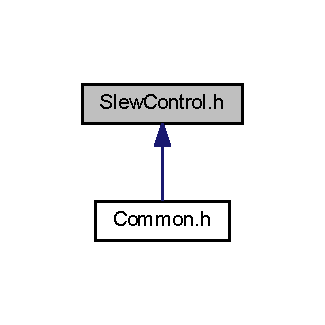
\includegraphics[width=150pt]{a00076}
\end{center}
\end{figure}
\subsection*{Typedefs}
\begin{DoxyCompactItemize}
\item 
typedef enum \hyperlink{a00047_aca06f1f459e3a5a5af6da9c575e60754}{slave\-Mode} \hyperlink{a00047_afb2b17d98c0aab4c05960f280d68084d}{slave\-Mode}
\end{DoxyCompactItemize}
\subsection*{Enumerations}
\begin{DoxyCompactItemize}
\item 
enum \hyperlink{a00047_aca06f1f459e3a5a5af6da9c575e60754}{slave\-Mode} 
\end{DoxyCompactItemize}
\subsection*{Functions}
\begin{DoxyCompactItemize}
\item 
\hyperlink{a00047_aca06f1f459e3a5a5af6da9c575e60754}{slave\-Mode} \hyperlink{a00047_ac6755edae0bbfd8297081fcdc57ec18f}{detect\-Slave\-Mode} (void)
\end{DoxyCompactItemize}
\subsection*{Variables}
\begin{DoxyCompactItemize}
\item 
\hyperlink{a00047_aca06f1f459e3a5a5af6da9c575e60754}{slave\-Mode} \hyperlink{a00047_a0fdda7865dd9c0be0eb545cb8234865a}{slave\-Mode\-Status}
\end{DoxyCompactItemize}


\subsection{Detailed Description}
Functions and variables used in detection of the mode of the unit. These functions determine the mode of the burn in unit and should be run after system start up. The detection is managed using G\-P\-I\-O6 and G\-P\-I\-O7. A unit may be in one of four modes\-: a single unit, a master unit, a slave unit or alternatively a unit may be in the undetected mode which is the initial mode of a unit upon startup.

\begin{DoxyWarning}{Warning}
For the mode to be correctly detected the two units should be connected while powered off, then the slave unit should be powered on first, followed by powering on the master unit second. Once detected at startup, any further changes to the connected mode will not be detected and thus the detected mode reported will not reflect such changes to the connection mode of the unit. To change the connection mode of a unit, it, and any slave or master unit must be powered off again.
\end{DoxyWarning}
Also note that, as mentioned, the mode detection algorithm uses G\-P\-I\-O6. However the during initialisation and use of the S\-P\-I peripheral G\-P\-I\-O6 is used as a slave service request line. Thus even if the unit mode is not used in conjunction with the S\-P\-I functions they should still only be used after the slave mode has been detected. 

\subsection{Typedef Documentation}
\hypertarget{a00047_afb2b17d98c0aab4c05960f280d68084d}{\index{slave\-Mode.\-h@{slave\-Mode.\-h}!slave\-Mode@{slave\-Mode}}
\index{slave\-Mode@{slave\-Mode}!slaveMode.h@{slave\-Mode.\-h}}
\subsubsection[{slave\-Mode}]{\setlength{\rightskip}{0pt plus 5cm}typedef enum {\bf slave\-Mode} {\bf slave\-Mode}}}\label{a00047_afb2b17d98c0aab4c05960f280d68084d}
A type to allow specification of the unit mode 

\subsection{Enumeration Type Documentation}
\hypertarget{a00047_aca06f1f459e3a5a5af6da9c575e60754}{\index{slave\-Mode.\-h@{slave\-Mode.\-h}!slave\-Mode@{slave\-Mode}}
\index{slave\-Mode@{slave\-Mode}!slaveMode.h@{slave\-Mode.\-h}}
\subsubsection[{slave\-Mode}]{\setlength{\rightskip}{0pt plus 5cm}enum {\bf slave\-Mode}}}\label{a00047_aca06f1f459e3a5a5af6da9c575e60754}
The possible unit modes 

\subsection{Function Documentation}
\hypertarget{a00047_ac6755edae0bbfd8297081fcdc57ec18f}{\index{slave\-Mode.\-h@{slave\-Mode.\-h}!detect\-Slave\-Mode@{detect\-Slave\-Mode}}
\index{detect\-Slave\-Mode@{detect\-Slave\-Mode}!slaveMode.h@{slave\-Mode.\-h}}
\subsubsection[{detect\-Slave\-Mode}]{\setlength{\rightskip}{0pt plus 5cm}{\bf slave\-Mode} detect\-Slave\-Mode (
\begin{DoxyParamCaption}
\item[{void}]{}
\end{DoxyParamCaption}
)}}\label{a00047_ac6755edae0bbfd8297081fcdc57ec18f}
Detects the unit mode. This should only be run once, at startup, to allow the mode to be provided to any other function initialisations that may rely on it.

When a slave unit is powered on the state of G\-P\-I\-O7 is read. If the reading is L\-O\-W, this indicates that the unit is a slave and subsequently G\-P\-I\-O6 is set H\-I\-G\-H. If the G\-P\-I\-O7 reading indicated that the unit is a master unit the state of G\-P\-I\-O6 is then read and if it is L\-O\-W it determines that the unit is a single unit.

\begin{DoxyReturn}{Returns}
The detected slave mode. If the mode has already been detected the state will be available by referencing the slave\-Mode\-Status variable instead. 
\end{DoxyReturn}


\subsection{Variable Documentation}
\hypertarget{a00047_a0fdda7865dd9c0be0eb545cb8234865a}{\index{slave\-Mode.\-h@{slave\-Mode.\-h}!slave\-Mode\-Status@{slave\-Mode\-Status}}
\index{slave\-Mode\-Status@{slave\-Mode\-Status}!slaveMode.h@{slave\-Mode.\-h}}
\subsubsection[{slave\-Mode\-Status}]{\setlength{\rightskip}{0pt plus 5cm}{\bf slave\-Mode} slave\-Mode\-Status}}\label{a00047_a0fdda7865dd9c0be0eb545cb8234865a}
A global variable that holds the detected mode of the unit, allowing the mode to be queried. 
\hypertarget{a00049}{\section{Slew\-Control.\-h File Reference}
\label{a00049}\index{Slew\-Control.\-h@{Slew\-Control.\-h}}
}


Slew control functions.  


This graph shows which files directly or indirectly include this file\-:
\nopagebreak
\begin{figure}[H]
\begin{center}
\leavevmode
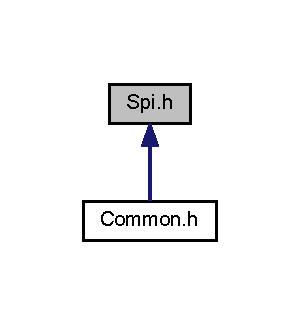
\includegraphics[width=156pt]{a00077}
\end{center}
\end{figure}
\subsection*{Functions}
\begin{DoxyCompactItemize}
\item 
void \hyperlink{a00049_a781fe23cb47009003e6d7b8343a377fa}{update\-Load\-Slew} (void)
\item 
Uint16 \hyperlink{a00049_af91ad2be323d5d0c10e6127418690811}{set\-Load\-Slew\-Target} (\hyperlink{a00027_a2820f1e18d921d2f1e97d53404b9fbae}{load\-Stage} load, float32 target)
\item 
Uint16 \hyperlink{a00049_ae38c51e6a504a6fd7a77edb6a3a06656}{set\-Load\-Slew\-Step} (\hyperlink{a00027_a2820f1e18d921d2f1e97d53404b9fbae}{load\-Stage} load, float32 step)
\item 
Uint16 \hyperlink{a00049_a567e736b557aa3dd69472d13f96ea006}{set\-Load\-State} (\hyperlink{a00027_a2820f1e18d921d2f1e97d53404b9fbae}{load\-Stage} load, Uint16 state)
\item 
Uint16 \hyperlink{a00049_a68d48d3f3c783662c131f2407f9e8792}{sc\-Set\-Load\-State\-All} (Uint16 state)
\item 
Uint16 \hyperlink{a00049_a90d0ebd5af992cd41a3fd3878e3d9b5a}{get\-Load\-Slew\-Target} (\hyperlink{a00027_a2820f1e18d921d2f1e97d53404b9fbae}{load\-Stage} load, float32 $\ast$target)
\item 
Uint16 \hyperlink{a00049_a33909c7bbfa64f91ef2257ecc97a8d7b}{get\-Load\-Slew\-Step} (\hyperlink{a00027_a2820f1e18d921d2f1e97d53404b9fbae}{load\-Stage} load, float32 $\ast$step)
\item 
Uint16 \hyperlink{a00049_af470a5cd45bfe44d75f6a314c45c256c}{get\-Load\-State} (\hyperlink{a00027_a2820f1e18d921d2f1e97d53404b9fbae}{load\-Stage} load, Uint16 $\ast$state)
\end{DoxyCompactItemize}


\subsection{Detailed Description}
Slew control functions. 

\subsection{Function Documentation}
\hypertarget{a00049_a33909c7bbfa64f91ef2257ecc97a8d7b}{\index{Slew\-Control.\-h@{Slew\-Control.\-h}!get\-Load\-Slew\-Step@{get\-Load\-Slew\-Step}}
\index{get\-Load\-Slew\-Step@{get\-Load\-Slew\-Step}!SlewControl.h@{Slew\-Control.\-h}}
\subsubsection[{get\-Load\-Slew\-Step}]{\setlength{\rightskip}{0pt plus 5cm}Uint16 get\-Load\-Slew\-Step (
\begin{DoxyParamCaption}
\item[{{\bf load\-Stage}}]{load, }
\item[{float32 $\ast$}]{step}
\end{DoxyParamCaption}
)}}\label{a00049_a33909c7bbfa64f91ef2257ecc97a8d7b}
Queries the current slew step size of the specified channel. 
\begin{DoxyParams}[1]{Parameters}
\mbox{\tt in}  & {\em load} & Specifies the load the setting is to be read from. \\
\hline
\mbox{\tt out}  & {\em step} & Pointer to location at which to place the query result (amps). \\
\hline
\end{DoxyParams}
\begin{DoxyReturn}{Returns}
Error status. 
\end{DoxyReturn}
\hypertarget{a00049_a90d0ebd5af992cd41a3fd3878e3d9b5a}{\index{Slew\-Control.\-h@{Slew\-Control.\-h}!get\-Load\-Slew\-Target@{get\-Load\-Slew\-Target}}
\index{get\-Load\-Slew\-Target@{get\-Load\-Slew\-Target}!SlewControl.h@{Slew\-Control.\-h}}
\subsubsection[{get\-Load\-Slew\-Target}]{\setlength{\rightskip}{0pt plus 5cm}Uint16 get\-Load\-Slew\-Target (
\begin{DoxyParamCaption}
\item[{{\bf load\-Stage}}]{load, }
\item[{float32 $\ast$}]{target}
\end{DoxyParamCaption}
)}}\label{a00049_a90d0ebd5af992cd41a3fd3878e3d9b5a}
Queries the current slew target setting for the specified channel. 
\begin{DoxyParams}[1]{Parameters}
\mbox{\tt in}  & {\em load} & Specifies the load the setting is to be read from. \\
\hline
\mbox{\tt out}  & {\em target} & Pointer to location at which to place the query result (amps). \\
\hline
\end{DoxyParams}
\begin{DoxyReturn}{Returns}
Error status. 
\end{DoxyReturn}
\hypertarget{a00049_af470a5cd45bfe44d75f6a314c45c256c}{\index{Slew\-Control.\-h@{Slew\-Control.\-h}!get\-Load\-State@{get\-Load\-State}}
\index{get\-Load\-State@{get\-Load\-State}!SlewControl.h@{Slew\-Control.\-h}}
\subsubsection[{get\-Load\-State}]{\setlength{\rightskip}{0pt plus 5cm}Uint16 get\-Load\-State (
\begin{DoxyParamCaption}
\item[{{\bf load\-Stage}}]{load, }
\item[{Uint16 $\ast$}]{state}
\end{DoxyParamCaption}
)}}\label{a00049_af470a5cd45bfe44d75f6a314c45c256c}
Queries the current reference net enable state for the specified channel. 
\begin{DoxyParams}[1]{Parameters}
\mbox{\tt in}  & {\em load} & Specifies the load the setting is to be read from. \\
\hline
\mbox{\tt out}  & {\em state} & Pointer to location at which to place the query result (0\-:O\-F\-F $|$ non-\/zero\-:O\-N). \\
\hline
\end{DoxyParams}
\begin{DoxyReturn}{Returns}
Error status. 
\end{DoxyReturn}
\hypertarget{a00049_a68d48d3f3c783662c131f2407f9e8792}{\index{Slew\-Control.\-h@{Slew\-Control.\-h}!sc\-Set\-Load\-State\-All@{sc\-Set\-Load\-State\-All}}
\index{sc\-Set\-Load\-State\-All@{sc\-Set\-Load\-State\-All}!SlewControl.h@{Slew\-Control.\-h}}
\subsubsection[{sc\-Set\-Load\-State\-All}]{\setlength{\rightskip}{0pt plus 5cm}Uint16 sc\-Set\-Load\-State\-All (
\begin{DoxyParamCaption}
\item[{Uint16}]{state}
\end{DoxyParamCaption}
)}}\label{a00049_a68d48d3f3c783662c131f2407f9e8792}
Sets all channels' reference net enable state. 
\begin{DoxyParams}[1]{Parameters}
\mbox{\tt in}  & {\em state} & Specifies the refernce net state to be applied (0\-:O\-F\-F $|$ non-\/zero\-:O\-N). \\
\hline
\end{DoxyParams}
\begin{DoxyReturn}{Returns}
Error status. 
\end{DoxyReturn}
\hypertarget{a00049_ae38c51e6a504a6fd7a77edb6a3a06656}{\index{Slew\-Control.\-h@{Slew\-Control.\-h}!set\-Load\-Slew\-Step@{set\-Load\-Slew\-Step}}
\index{set\-Load\-Slew\-Step@{set\-Load\-Slew\-Step}!SlewControl.h@{Slew\-Control.\-h}}
\subsubsection[{set\-Load\-Slew\-Step}]{\setlength{\rightskip}{0pt plus 5cm}Uint16 set\-Load\-Slew\-Step (
\begin{DoxyParamCaption}
\item[{{\bf load\-Stage}}]{load, }
\item[{float32}]{step}
\end{DoxyParamCaption}
)}}\label{a00049_ae38c51e6a504a6fd7a77edb6a3a06656}
Sets the slew step size for the specified load. 
\begin{DoxyParams}[1]{Parameters}
\mbox{\tt in}  & {\em load} & Specifies the load the setting is to be applied to. \\
\hline
\mbox{\tt in}  & {\em step} & Specifies the value of the slew step size to be applied (amps). \\
\hline
\end{DoxyParams}
\begin{DoxyReturn}{Returns}
Error status. 
\end{DoxyReturn}
\hypertarget{a00049_af91ad2be323d5d0c10e6127418690811}{\index{Slew\-Control.\-h@{Slew\-Control.\-h}!set\-Load\-Slew\-Target@{set\-Load\-Slew\-Target}}
\index{set\-Load\-Slew\-Target@{set\-Load\-Slew\-Target}!SlewControl.h@{Slew\-Control.\-h}}
\subsubsection[{set\-Load\-Slew\-Target}]{\setlength{\rightskip}{0pt plus 5cm}Uint16 set\-Load\-Slew\-Target (
\begin{DoxyParamCaption}
\item[{{\bf load\-Stage}}]{load, }
\item[{float32}]{target}
\end{DoxyParamCaption}
)}}\label{a00049_af91ad2be323d5d0c10e6127418690811}
Sets the slew target for the specified load. 
\begin{DoxyParams}[1]{Parameters}
\mbox{\tt in}  & {\em load} & Specifies the load the setting is to be applied to. \\
\hline
\mbox{\tt in}  & {\em target} & Specifies the value of the slew target to be applied (amps). \\
\hline
\end{DoxyParams}
\begin{DoxyReturn}{Returns}
Error status. 
\end{DoxyReturn}
\hypertarget{a00049_a567e736b557aa3dd69472d13f96ea006}{\index{Slew\-Control.\-h@{Slew\-Control.\-h}!set\-Load\-State@{set\-Load\-State}}
\index{set\-Load\-State@{set\-Load\-State}!SlewControl.h@{Slew\-Control.\-h}}
\subsubsection[{set\-Load\-State}]{\setlength{\rightskip}{0pt plus 5cm}Uint16 set\-Load\-State (
\begin{DoxyParamCaption}
\item[{{\bf load\-Stage}}]{load, }
\item[{Uint16}]{state}
\end{DoxyParamCaption}
)}}\label{a00049_a567e736b557aa3dd69472d13f96ea006}
Sets the reference net enable state for the specified load. 
\begin{DoxyParams}[1]{Parameters}
\mbox{\tt in}  & {\em load} & Specifies the load the setting is to be applied to. \\
\hline
\mbox{\tt in}  & {\em state} & Specifies the reference net state to be applied (0\-:O\-F\-F $|$ non-\/zero\-:O\-N). \\
\hline
\end{DoxyParams}
\begin{DoxyReturn}{Returns}
Error Status. 
\end{DoxyReturn}
\hypertarget{a00049_a781fe23cb47009003e6d7b8343a377fa}{\index{Slew\-Control.\-h@{Slew\-Control.\-h}!update\-Load\-Slew@{update\-Load\-Slew}}
\index{update\-Load\-Slew@{update\-Load\-Slew}!SlewControl.h@{Slew\-Control.\-h}}
\subsubsection[{update\-Load\-Slew}]{\setlength{\rightskip}{0pt plus 5cm}void update\-Load\-Slew (
\begin{DoxyParamCaption}
\item[{void}]{}
\end{DoxyParamCaption}
)}}\label{a00049_a781fe23cb47009003e6d7b8343a377fa}
Advances the slew ramps for all loads. 
\hypertarget{a00051}{\section{Spi.\-h File Reference}
\label{a00051}\index{Spi.\-h@{Spi.\-h}}
}


Serial peripheral interface communications functions.  


This graph shows which files directly or indirectly include this file\-:
\nopagebreak
\begin{figure}[H]
\begin{center}
\leavevmode
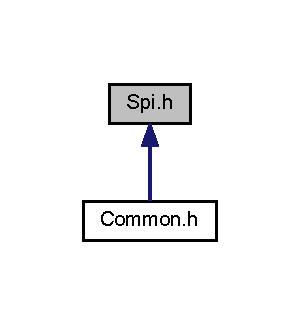
\includegraphics[width=144pt]{a00078}
\end{center}
\end{figure}
\subsection*{Macros}
\begin{DoxyCompactItemize}
\item 
\#define \hyperlink{a00051_a02b50bd3a63177b3074b0aa1ed813e38}{S\-P\-I\-\_\-\-D\-F\-L\-T\-\_\-\-B\-A\-U\-D}~0x3\-D090
\item 
\#define \hyperlink{a00051_a203ac5cf3a2f7ee6932c53909a2b41e8}{S\-P\-I\-\_\-\-D\-F\-L\-T\-\_\-\-C\-P\-O\-L}~0x00
\item 
\#define \hyperlink{a00051_a8ef22e1c92c431c764876c93a6e53f40}{S\-P\-I\-\_\-\-D\-F\-L\-T\-\_\-\-C\-P\-H\-A}~0x01
\item 
\#define \hyperlink{a00051_aaf3e602cf02d489821651ca9ee6774ea}{S\-P\-I\-\_\-\-F\-F\-R\-X\-\_\-\-I\-N\-T\-L\-V\-L}~0x01
\item 
\#define \hyperlink{a00051_a2e13bd89cf02fafba0287ffca964b102}{S\-P\-I\-\_\-\-F\-F\-T\-X\-\_\-\-I\-N\-T\-L\-V\-L}~0x00
\item 
\#define \hyperlink{a00051_a38b4bec17e21d86050db6fa1f5ec6f33}{S\-P\-I\-\_\-\-F\-F\-T\-X\-\_\-\-F\-I\-L\-L\-V\-L}~0x04
\end{DoxyCompactItemize}
\subsection*{Typedefs}
\begin{DoxyCompactItemize}
\item 
typedef enum \hyperlink{a00051_afb5b84cea8395f82ed709dbd8dcc82ce}{spi\-Mode} \hyperlink{a00051_a6707561b1d595f87f0cf027cdc4f262d}{spi\-Mode}
\item 
typedef enum \hyperlink{a00051_ab94a5ba6760c1a12ee032dd12fffd6a3}{spi\-Lpbk} \hyperlink{a00051_a2709984dcd2ad90d6c4066b0d8d0769a}{spi\-Lpbk}
\item 
typedef enum \hyperlink{a00051_ab694d7b7f6041ac353aa1475e9c39ddc}{trans\-Pol} \hyperlink{a00051_a9d877f7feaeca9d2393e8dbae1aca73d}{trans\-Pol}
\item 
typedef enum \hyperlink{a00051_a0701b982f4dc80e47f32c3419a27f1d9}{spi\-C\-Pha} \hyperlink{a00051_aed8a0ae18613612fe7700f5da26144ba}{spi\-C\-Pha}
\end{DoxyCompactItemize}
\subsection*{Enumerations}
\begin{DoxyCompactItemize}
\item 
enum \hyperlink{a00051_afb5b84cea8395f82ed709dbd8dcc82ce}{spi\-Mode} 
\item 
enum \hyperlink{a00051_ab94a5ba6760c1a12ee032dd12fffd6a3}{spi\-Lpbk} 
\item 
enum \hyperlink{a00051_ab694d7b7f6041ac353aa1475e9c39ddc}{trans\-Pol} 
\item 
enum \hyperlink{a00051_a0701b982f4dc80e47f32c3419a27f1d9}{spi\-C\-Pha} 
\end{DoxyCompactItemize}
\subsection*{Functions}
\begin{DoxyCompactItemize}
\item 
Uint16 \hyperlink{a00051_af60691ee5cb4ab20b305278c6e435511}{spi\-Init} (\hyperlink{a00051_afb5b84cea8395f82ed709dbd8dcc82ce}{spi\-Mode} mode, Uint32 baud, \hyperlink{a00051_ab94a5ba6760c1a12ee032dd12fffd6a3}{spi\-Lpbk} loopback, \hyperlink{a00051_ab694d7b7f6041ac353aa1475e9c39ddc}{trans\-Pol} c\-Pol, \hyperlink{a00051_a0701b982f4dc80e47f32c3419a27f1d9}{spi\-C\-Pha} c\-Pha)
\item 
void \hyperlink{a00051_a2a410bb43bd6e77aa27484add35a009d}{spi\-Tx} (void)
\end{DoxyCompactItemize}


\subsection{Detailed Description}
Serial peripheral interface communications functions. As a master G\-P\-I\-O6 is setup as external interrupt 2 for the slave service request line, set as active low. As a master G\-P\-I\-O6 is setup as an active low output.

\begin{DoxyWarning}{Warning}
The following bridge tracks should be cut on the T\-I C2000 Launch\-Pad X\-L P\-C\-B before S\-P\-I (or I2\-C) may be used\-: \begin{TabularC}{3}
\hline
\rowcolor{lightgray}\PBS\centering {\bf Bridge to Cut }&\PBS\centering {\bf G\-P\-I\-O }&\PBS\centering {\bf P\-C\-B Pin  }\\\cline{1-3}
\PBS\centering J\-P5 &\PBS\centering G\-P\-I\-O32&\PBS\centering J2-\/6 \\\cline{1-3}
\PBS\centering J\-P7 &\PBS\centering G\-P\-I\-O33&\PBS\centering J2-\/7 \\\cline{1-3}
\PBS\centering J\-P8 &\PBS\centering G\-P\-I\-O16&\PBS\centering J6-\/7 \\\cline{1-3}
\PBS\centering J\-P10 &\PBS\centering G\-P\-I\-O17&\PBS\centering J6-\/8 \\\cline{1-3}
\end{TabularC}
This should result in the following functionality\-: \begin{TabularC}{3}
\hline
\rowcolor{lightgray}\PBS\centering {\bf Function }&\PBS\centering {\bf G\-P\-I\-O }&\PBS\centering {\bf P\-C\-B Pin  }\\\cline{1-3}
\PBS\centering I2\-C\-\_\-\-S\-D\-A\-A &\PBS\centering G\-P\-I\-O32&\PBS\centering J6-\/7 \\\cline{1-3}
\PBS\centering I2\-C\-\_\-\-S\-C\-L\-A &\PBS\centering G\-P\-I\-O33&\PBS\centering J6-\/8 \\\cline{1-3}
\PBS\centering S\-P\-I\-\_\-\-M\-O\-S\-I &\PBS\centering G\-P\-I\-O16&\PBS\centering J2-\/6 \\\cline{1-3}
\PBS\centering S\-P\-I\-\_\-\-M\-I\-S\-O &\PBS\centering G\-P\-I\-O17&\PBS\centering J2-\/7 \\\cline{1-3}
\PBS\centering S\-P\-I\-\_\-\-C\-L\-K &\PBS\centering G\-P\-I\-O18&\PBS\centering J1-\/18 \\\cline{1-3}
\PBS\centering S\-P\-I\-\_\-\-S\-T\-E &\PBS\centering G\-P\-I\-O19&\PBS\centering J2-\/1 \\\cline{1-3}
\end{TabularC}

\end{DoxyWarning}


\subsection{Macro Definition Documentation}
\hypertarget{a00051_a02b50bd3a63177b3074b0aa1ed813e38}{\index{Spi.\-h@{Spi.\-h}!S\-P\-I\-\_\-\-D\-F\-L\-T\-\_\-\-B\-A\-U\-D@{S\-P\-I\-\_\-\-D\-F\-L\-T\-\_\-\-B\-A\-U\-D}}
\index{S\-P\-I\-\_\-\-D\-F\-L\-T\-\_\-\-B\-A\-U\-D@{S\-P\-I\-\_\-\-D\-F\-L\-T\-\_\-\-B\-A\-U\-D}!Spi.h@{Spi.\-h}}
\subsubsection[{S\-P\-I\-\_\-\-D\-F\-L\-T\-\_\-\-B\-A\-U\-D}]{\setlength{\rightskip}{0pt plus 5cm}\#define S\-P\-I\-\_\-\-D\-F\-L\-T\-\_\-\-B\-A\-U\-D~0x3\-D090}}\label{a00051_a02b50bd3a63177b3074b0aa1ed813e38}
S\-P\-I default baud rate. \hypertarget{a00051_a8ef22e1c92c431c764876c93a6e53f40}{\index{Spi.\-h@{Spi.\-h}!S\-P\-I\-\_\-\-D\-F\-L\-T\-\_\-\-C\-P\-H\-A@{S\-P\-I\-\_\-\-D\-F\-L\-T\-\_\-\-C\-P\-H\-A}}
\index{S\-P\-I\-\_\-\-D\-F\-L\-T\-\_\-\-C\-P\-H\-A@{S\-P\-I\-\_\-\-D\-F\-L\-T\-\_\-\-C\-P\-H\-A}!Spi.h@{Spi.\-h}}
\subsubsection[{S\-P\-I\-\_\-\-D\-F\-L\-T\-\_\-\-C\-P\-H\-A}]{\setlength{\rightskip}{0pt plus 5cm}\#define S\-P\-I\-\_\-\-D\-F\-L\-T\-\_\-\-C\-P\-H\-A~0x01}}\label{a00051_a8ef22e1c92c431c764876c93a6e53f40}
S\-P\-I default clock phase. 0 = Without delay, 1 = with delay. \hypertarget{a00051_a203ac5cf3a2f7ee6932c53909a2b41e8}{\index{Spi.\-h@{Spi.\-h}!S\-P\-I\-\_\-\-D\-F\-L\-T\-\_\-\-C\-P\-O\-L@{S\-P\-I\-\_\-\-D\-F\-L\-T\-\_\-\-C\-P\-O\-L}}
\index{S\-P\-I\-\_\-\-D\-F\-L\-T\-\_\-\-C\-P\-O\-L@{S\-P\-I\-\_\-\-D\-F\-L\-T\-\_\-\-C\-P\-O\-L}!Spi.h@{Spi.\-h}}
\subsubsection[{S\-P\-I\-\_\-\-D\-F\-L\-T\-\_\-\-C\-P\-O\-L}]{\setlength{\rightskip}{0pt plus 5cm}\#define S\-P\-I\-\_\-\-D\-F\-L\-T\-\_\-\-C\-P\-O\-L~0x00}}\label{a00051_a203ac5cf3a2f7ee6932c53909a2b41e8}
S\-P\-I default clock polarity. 0 = Rising edge, 1 = falling edge. \hypertarget{a00051_aaf3e602cf02d489821651ca9ee6774ea}{\index{Spi.\-h@{Spi.\-h}!S\-P\-I\-\_\-\-F\-F\-R\-X\-\_\-\-I\-N\-T\-L\-V\-L@{S\-P\-I\-\_\-\-F\-F\-R\-X\-\_\-\-I\-N\-T\-L\-V\-L}}
\index{S\-P\-I\-\_\-\-F\-F\-R\-X\-\_\-\-I\-N\-T\-L\-V\-L@{S\-P\-I\-\_\-\-F\-F\-R\-X\-\_\-\-I\-N\-T\-L\-V\-L}!Spi.h@{Spi.\-h}}
\subsubsection[{S\-P\-I\-\_\-\-F\-F\-R\-X\-\_\-\-I\-N\-T\-L\-V\-L}]{\setlength{\rightskip}{0pt plus 5cm}\#define S\-P\-I\-\_\-\-F\-F\-R\-X\-\_\-\-I\-N\-T\-L\-V\-L~0x01}}\label{a00051_aaf3e602cf02d489821651ca9ee6774ea}
S\-P\-I Rx F\-I\-F\-O interrupt level. \hypertarget{a00051_a38b4bec17e21d86050db6fa1f5ec6f33}{\index{Spi.\-h@{Spi.\-h}!S\-P\-I\-\_\-\-F\-F\-T\-X\-\_\-\-F\-I\-L\-L\-V\-L@{S\-P\-I\-\_\-\-F\-F\-T\-X\-\_\-\-F\-I\-L\-L\-V\-L}}
\index{S\-P\-I\-\_\-\-F\-F\-T\-X\-\_\-\-F\-I\-L\-L\-V\-L@{S\-P\-I\-\_\-\-F\-F\-T\-X\-\_\-\-F\-I\-L\-L\-V\-L}!Spi.h@{Spi.\-h}}
\subsubsection[{S\-P\-I\-\_\-\-F\-F\-T\-X\-\_\-\-F\-I\-L\-L\-V\-L}]{\setlength{\rightskip}{0pt plus 5cm}\#define S\-P\-I\-\_\-\-F\-F\-T\-X\-\_\-\-F\-I\-L\-L\-V\-L~0x04}}\label{a00051_a38b4bec17e21d86050db6fa1f5ec6f33}
S\-P\-I Tx F\-I\-F\-O fill level. \hypertarget{a00051_a2e13bd89cf02fafba0287ffca964b102}{\index{Spi.\-h@{Spi.\-h}!S\-P\-I\-\_\-\-F\-F\-T\-X\-\_\-\-I\-N\-T\-L\-V\-L@{S\-P\-I\-\_\-\-F\-F\-T\-X\-\_\-\-I\-N\-T\-L\-V\-L}}
\index{S\-P\-I\-\_\-\-F\-F\-T\-X\-\_\-\-I\-N\-T\-L\-V\-L@{S\-P\-I\-\_\-\-F\-F\-T\-X\-\_\-\-I\-N\-T\-L\-V\-L}!Spi.h@{Spi.\-h}}
\subsubsection[{S\-P\-I\-\_\-\-F\-F\-T\-X\-\_\-\-I\-N\-T\-L\-V\-L}]{\setlength{\rightskip}{0pt plus 5cm}\#define S\-P\-I\-\_\-\-F\-F\-T\-X\-\_\-\-I\-N\-T\-L\-V\-L~0x00}}\label{a00051_a2e13bd89cf02fafba0287ffca964b102}
S\-P\-I Tx F\-I\-F\-O interrupt level. 

\subsection{Typedef Documentation}
\hypertarget{a00051_aed8a0ae18613612fe7700f5da26144ba}{\index{Spi.\-h@{Spi.\-h}!spi\-C\-Pha@{spi\-C\-Pha}}
\index{spi\-C\-Pha@{spi\-C\-Pha}!Spi.h@{Spi.\-h}}
\subsubsection[{spi\-C\-Pha}]{\setlength{\rightskip}{0pt plus 5cm}typedef enum {\bf spi\-C\-Pha} {\bf spi\-C\-Pha}}}\label{a00051_aed8a0ae18613612fe7700f5da26144ba}
A type to allow specification of the S\-P\-I clock phase setting. \hypertarget{a00051_a2709984dcd2ad90d6c4066b0d8d0769a}{\index{Spi.\-h@{Spi.\-h}!spi\-Lpbk@{spi\-Lpbk}}
\index{spi\-Lpbk@{spi\-Lpbk}!Spi.h@{Spi.\-h}}
\subsubsection[{spi\-Lpbk}]{\setlength{\rightskip}{0pt plus 5cm}typedef enum {\bf spi\-Lpbk} {\bf spi\-Lpbk}}}\label{a00051_a2709984dcd2ad90d6c4066b0d8d0769a}
A type to allows specification of the S\-P\-I loop-\/back setting. \hypertarget{a00051_a6707561b1d595f87f0cf027cdc4f262d}{\index{Spi.\-h@{Spi.\-h}!spi\-Mode@{spi\-Mode}}
\index{spi\-Mode@{spi\-Mode}!Spi.h@{Spi.\-h}}
\subsubsection[{spi\-Mode}]{\setlength{\rightskip}{0pt plus 5cm}typedef enum {\bf spi\-Mode} {\bf spi\-Mode}}}\label{a00051_a6707561b1d595f87f0cf027cdc4f262d}
A type to allow specification of the S\-P\-I mode. \hypertarget{a00051_a9d877f7feaeca9d2393e8dbae1aca73d}{\index{Spi.\-h@{Spi.\-h}!trans\-Pol@{trans\-Pol}}
\index{trans\-Pol@{trans\-Pol}!Spi.h@{Spi.\-h}}
\subsubsection[{trans\-Pol}]{\setlength{\rightskip}{0pt plus 5cm}typedef enum {\bf trans\-Pol} {\bf trans\-Pol}}}\label{a00051_a9d877f7feaeca9d2393e8dbae1aca73d}
A type to allow specification of the edge transition polarity setting. 

\subsection{Enumeration Type Documentation}
\hypertarget{a00051_a0701b982f4dc80e47f32c3419a27f1d9}{\index{Spi.\-h@{Spi.\-h}!spi\-C\-Pha@{spi\-C\-Pha}}
\index{spi\-C\-Pha@{spi\-C\-Pha}!Spi.h@{Spi.\-h}}
\subsubsection[{spi\-C\-Pha}]{\setlength{\rightskip}{0pt plus 5cm}enum {\bf spi\-C\-Pha}}}\label{a00051_a0701b982f4dc80e47f32c3419a27f1d9}
The possible S\-P\-I clock phase settings. \hypertarget{a00051_ab94a5ba6760c1a12ee032dd12fffd6a3}{\index{Spi.\-h@{Spi.\-h}!spi\-Lpbk@{spi\-Lpbk}}
\index{spi\-Lpbk@{spi\-Lpbk}!Spi.h@{Spi.\-h}}
\subsubsection[{spi\-Lpbk}]{\setlength{\rightskip}{0pt plus 5cm}enum {\bf spi\-Lpbk}}}\label{a00051_ab94a5ba6760c1a12ee032dd12fffd6a3}
The possible S\-P\-I loop-\/back settings. \hypertarget{a00051_afb5b84cea8395f82ed709dbd8dcc82ce}{\index{Spi.\-h@{Spi.\-h}!spi\-Mode@{spi\-Mode}}
\index{spi\-Mode@{spi\-Mode}!Spi.h@{Spi.\-h}}
\subsubsection[{spi\-Mode}]{\setlength{\rightskip}{0pt plus 5cm}enum {\bf spi\-Mode}}}\label{a00051_afb5b84cea8395f82ed709dbd8dcc82ce}
The possible S\-P\-I Modes. \hypertarget{a00051_ab694d7b7f6041ac353aa1475e9c39ddc}{\index{Spi.\-h@{Spi.\-h}!trans\-Pol@{trans\-Pol}}
\index{trans\-Pol@{trans\-Pol}!Spi.h@{Spi.\-h}}
\subsubsection[{trans\-Pol}]{\setlength{\rightskip}{0pt plus 5cm}enum {\bf trans\-Pol}}}\label{a00051_ab694d7b7f6041ac353aa1475e9c39ddc}
The possible edge transition polarity settings. 

\subsection{Function Documentation}
\hypertarget{a00051_af60691ee5cb4ab20b305278c6e435511}{\index{Spi.\-h@{Spi.\-h}!spi\-Init@{spi\-Init}}
\index{spi\-Init@{spi\-Init}!Spi.h@{Spi.\-h}}
\subsubsection[{spi\-Init}]{\setlength{\rightskip}{0pt plus 5cm}Uint16 spi\-Init (
\begin{DoxyParamCaption}
\item[{{\bf spi\-Mode}}]{mode, }
\item[{Uint32}]{baud, }
\item[{{\bf spi\-Lpbk}}]{loopback, }
\item[{{\bf trans\-Pol}}]{c\-Pol, }
\item[{{\bf spi\-C\-Pha}}]{c\-Pha}
\end{DoxyParamCaption}
)}}\label{a00051_af60691ee5cb4ab20b305278c6e435511}
Initialises the S\-P\-I-\/\-A peripheral and relevant interrupts 
\begin{DoxyParams}[1]{Parameters}
\mbox{\tt in}  & {\em mode} & Specifies if the device is in slave or master mode, values are master or slave. \\
\hline
\mbox{\tt in}  & {\em baud} & Specifies the baud rate to be used minimum value is 117,187, maximum is 3,750,000 \\
\hline
\mbox{\tt in}  & {\em loopback} & Specifies if the S\-P\-I module should be run in loop-\/back mode, values are enable or disable. \\
\hline
\mbox{\tt in}  & {\em c\-Pol} & Specifies the clock polarity, values are rising\-Edge or falling\-Edge. \\
\hline
\mbox{\tt in}  & {\em c\-Pha} & Specifies the clock phase, values are with\-Delay or without\-Delay. \\
\hline
\end{DoxyParams}
\begin{DoxyReturn}{Returns}
Error status.
\end{DoxyReturn}
\begin{DoxyWarning}{Warning}
This function will clear any values already in the S\-P\-I peripheral registers. 

This function M\-U\-S\-T be called before any other public S\-P\-I function. 
\end{DoxyWarning}
\hypertarget{a00051_a2a410bb43bd6e77aa27484add35a009d}{\index{Spi.\-h@{Spi.\-h}!spi\-Tx@{spi\-Tx}}
\index{spi\-Tx@{spi\-Tx}!Spi.h@{Spi.\-h}}
\subsubsection[{spi\-Tx}]{\setlength{\rightskip}{0pt plus 5cm}void spi\-Tx (
\begin{DoxyParamCaption}
\item[{void}]{}
\end{DoxyParamCaption}
)}}\label{a00051_a2a410bb43bd6e77aa27484add35a009d}
Transmits whatever data is on the S\-C\-P\-I output queue if S\-P\-I has been selected as the external communications type. 
\hypertarget{a00054}{\section{State\-Machine.\-h File Reference}
\label{a00054}\index{State\-Machine.\-h@{State\-Machine.\-h}}
}


State machine functions.  


This graph shows which files directly or indirectly include this file\-:\nopagebreak
\begin{figure}[H]
\begin{center}
\leavevmode
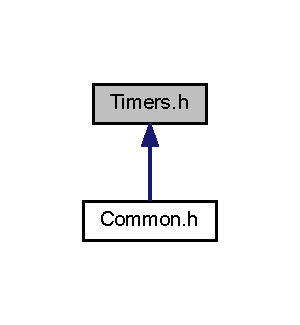
\includegraphics[width=164pt]{a00079}
\end{center}
\end{figure}
\subsection*{Functions}
\begin{DoxyCompactItemize}
\item 
void \hyperlink{a00054_ae3193cfcdfecbf55af42586e4c12a6e7}{init\-State\-Machine} (void)
\end{DoxyCompactItemize}
\subsection*{Variables}
\begin{DoxyCompactItemize}
\item 
void($\ast$ \hyperlink{a00054_af1d16f7a57d6ced065765dcbb355fcde}{Alpha\-\_\-\-State\-\_\-\-Ptr} )(void)
\end{DoxyCompactItemize}


\subsection{Detailed Description}
State machine functions. 

\subsection{Function Documentation}
\hypertarget{a00054_ae3193cfcdfecbf55af42586e4c12a6e7}{\index{State\-Machine.\-h@{State\-Machine.\-h}!init\-State\-Machine@{init\-State\-Machine}}
\index{init\-State\-Machine@{init\-State\-Machine}!StateMachine.h@{State\-Machine.\-h}}
\subsubsection[{init\-State\-Machine}]{\setlength{\rightskip}{0pt plus 5cm}void init\-State\-Machine (
\begin{DoxyParamCaption}
\item[{void}]{}
\end{DoxyParamCaption}
)}}\label{a00054_ae3193cfcdfecbf55af42586e4c12a6e7}
Sets up the state machine (including timers) ready for use. 

\subsection{Variable Documentation}
\hypertarget{a00054_af1d16f7a57d6ced065765dcbb355fcde}{\index{State\-Machine.\-h@{State\-Machine.\-h}!Alpha\-\_\-\-State\-\_\-\-Ptr@{Alpha\-\_\-\-State\-\_\-\-Ptr}}
\index{Alpha\-\_\-\-State\-\_\-\-Ptr@{Alpha\-\_\-\-State\-\_\-\-Ptr}!StateMachine.h@{State\-Machine.\-h}}
\subsubsection[{Alpha\-\_\-\-State\-\_\-\-Ptr}]{\setlength{\rightskip}{0pt plus 5cm}void($\ast$ Alpha\-\_\-\-State\-\_\-\-Ptr)(void)}}\label{a00054_af1d16f7a57d6ced065765dcbb355fcde}
Runs the next iteration of the state machine. Should be called from the main super-\/loop. 
\hypertarget{a00056}{\section{Timers.\-h File Reference}
\label{a00056}\index{Timers.\-h@{Timers.\-h}}
}


Real and virtual timer functions.  


This graph shows which files directly or indirectly include this file\-:
\nopagebreak
\begin{figure}[H]
\begin{center}
\leavevmode
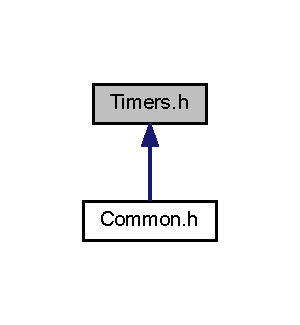
\includegraphics[width=144pt]{a00080}
\end{center}
\end{figure}
\subsection*{Functions}
\begin{DoxyCompactItemize}
\item 
void \hyperlink{a00056_a366f5c2927c6a77c9704bee58468a042}{timers\-Setup\-Real} (void)
\end{DoxyCompactItemize}


\subsection{Detailed Description}
Real and virtual timer functions. These functions should be run as part of the state machine setup.

\begin{DoxySeeAlso}{See Also}
\hyperlink{a00054}{State\-Machine.\-h} 
\end{DoxySeeAlso}


\subsection{Function Documentation}
\hypertarget{a00056_a366f5c2927c6a77c9704bee58468a042}{\index{Timers.\-h@{Timers.\-h}!timers\-Setup\-Real@{timers\-Setup\-Real}}
\index{timers\-Setup\-Real@{timers\-Setup\-Real}!Timers.h@{Timers.\-h}}
\subsubsection[{timers\-Setup\-Real}]{\setlength{\rightskip}{0pt plus 5cm}void timers\-Setup\-Real (
\begin{DoxyParamCaption}
\item[{void}]{}
\end{DoxyParamCaption}
)}}\label{a00056_a366f5c2927c6a77c9704bee58468a042}
Sets up the real timers that run the state machine This should be called as part of the state machine initialisation. \begin{DoxySeeAlso}{See Also}
sm\-Init() 
\end{DoxySeeAlso}

\hypertarget{a00058}{\section{Tmp.\-h File Reference}
\label{a00058}\index{Tmp.\-h@{Tmp.\-h}}
}


Temperature sensor functions.  


This graph shows which files directly or indirectly include this file\-:
\nopagebreak
\begin{figure}[H]
\begin{center}
\leavevmode
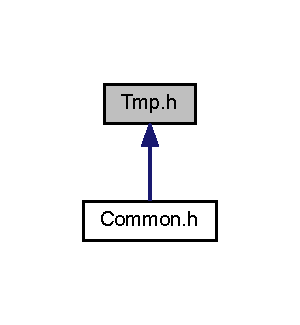
\includegraphics[width=144pt]{a00081}
\end{center}
\end{figure}
\subsection*{Macros}
\begin{DoxyCompactItemize}
\item 
\#define \hyperlink{a00058_ac80e67c94bf6570094bba2248b9586f3}{A\-D\-C\-\_\-\-S\-W3\-A\-\_\-\-S\-T\-A\-T\-E}~0x00
\item 
\#define \hyperlink{a00058_a63e298aff78f6afee6ebffa60c1de62a}{A\-D\-C\-\_\-\-S\-W3\-B\-\_\-\-S\-T\-A\-T\-E}~0x00
\item 
\#define \hyperlink{a00058_a6c0e4f915b6ac0c3af9a27d604f1f7b1}{A\-D\-C\-\_\-\-I2\-C\-\_\-\-B\-A\-S\-E\-\_\-\-A\-D\-D\-R}~0x48
\item 
\#define \hyperlink{a00058_a5fd3aabe18504a5314a5d0e71e3bc495}{A\-D\-C\-\_\-\-I2\-C\-\_\-\-A\-D\-D\-R}~(\hyperlink{a00058_a6c0e4f915b6ac0c3af9a27d604f1f7b1}{A\-D\-C\-\_\-\-I2\-C\-\_\-\-B\-A\-S\-E\-\_\-\-A\-D\-D\-R} $|$ \hyperlink{a00058_ac80e67c94bf6570094bba2248b9586f3}{A\-D\-C\-\_\-\-S\-W3\-A\-\_\-\-S\-T\-A\-T\-E}) $|$ (\hyperlink{a00058_a63e298aff78f6afee6ebffa60c1de62a}{A\-D\-C\-\_\-\-S\-W3\-B\-\_\-\-S\-T\-A\-T\-E} $<$$<$ 1)
\item 
\#define \hyperlink{a00058_a448e8a52be570dfe9fdddb2045039534}{A\-D\-C\-\_\-\-N\-U\-M\-\_\-\-C\-H\-N\-L}~0x08
\item 
\#define \hyperlink{a00058_a5a03d0b939a8dda552c9fe3319a82485}{A\-D\-C\-\_\-\-V\-R\-E\-F}~5.\-0
\item 
\#define \hyperlink{a00058_a9be6401f8c9339711816bec5ca55dd88}{A\-D\-C\-\_\-\-S\-T\-P\-S}~256
\item 
\#define \hyperlink{a00058_a6d41a70e126c748f2c99c3ff8228eb1b}{T\-M\-P\-\_\-\-V0\-C\-\_\-\-O\-F\-S\-T}~0.\-4
\item 
\#define \hyperlink{a00058_a0f910bb108922c8686a139977510af53}{T\-M\-P\-\_\-\-S\-C\-L\-\_\-\-O\-F\-S\-T}~\hyperlink{a00058_a6d41a70e126c748f2c99c3ff8228eb1b}{T\-M\-P\-\_\-\-V0\-C\-\_\-\-O\-F\-S\-T} $\ast$ \hyperlink{a00058_a9be6401f8c9339711816bec5ca55dd88}{A\-D\-C\-\_\-\-S\-T\-P\-S} / \hyperlink{a00058_a5a03d0b939a8dda552c9fe3319a82485}{A\-D\-C\-\_\-\-V\-R\-E\-F}
\item 
\#define \hyperlink{a00058_acc66f9f90ea4746679f5d26c834ddea5}{T\-M\-P\-\_\-\-E\-\_\-\-T\-\_\-\-C\-O\-L\-D}~1.\-5
\end{DoxyCompactItemize}
\subsection*{Functions}
\begin{DoxyCompactItemize}
\item 
Uint16 \hyperlink{a00058_a3e441d5071e094ff4f2aeb9d47f9a102}{init\-Temperature} (void)
\item 
Uint16 \hyperlink{a00058_a74292ec2fc953664dbf7be82f1656b09}{read\-Temperature} (Uint16 chnl, float32 $\ast$tmp\-Dest)
\end{DoxyCompactItemize}


\subsection{Detailed Description}
Temperature sensor functions. The temperature sensor (M\-C\-P9701) output is read via an external A\-D\-C (A\-D\-S7830) that is connected to the I2\-C bus at address 10010xx where 'xx' is dependent upon the state of switch 3 (S\-W3) on the Ctrl P\-C\-B, which the user should record in the macros A\-D\-C\-\_\-\-S\-W3\-A\-\_\-\-S\-T\-A\-T\-E and A\-D\-C\-\_\-\-S\-W3\-B\-\_\-\-S\-T\-A\-T\-E.

All temperatures are in degrees Celsius.

\begin{DoxyWarning}{Warning}
Before any temperature functions can be used the I2\-C peripheral M\-U\-S\-T be initialised, using i2c\-Init(), and \hyperlink{a00058_a3e441d5071e094ff4f2aeb9d47f9a102}{init\-Temperature()} must be run -\/ \hyperlink{a00058_a3e441d5071e094ff4f2aeb9d47f9a102}{init\-Temperature()} will require the interrupts to be enabled globally.
\end{DoxyWarning}
\begin{DoxySeeAlso}{See Also}
i2c\-Init()
\end{DoxySeeAlso}
\begin{TabularC}{4}
\hline
\rowcolor{lightgray}\PBS\centering {\bf A\-D\-S7830 Ch \#}&\PBS\centering {\bf Signal }&\PBS\centering {\bf Chnl selector }&\PBS\centering {\bf A\-D\-C Sel Code  }\\\cline{1-4}
\PBS\centering C\-H0 &\PBS\centering T\-E\-M\-P1 &\PBS\centering load1 (0) &\PBS\centering 0 \\\cline{1-4}
\PBS\centering C\-H1 &\PBS\centering T\-E\-M\-P2 &\PBS\centering load2 (1) &\PBS\centering 4 \\\cline{1-4}
\PBS\centering C\-H2 &\PBS\centering T\-E\-M\-P3 &\PBS\centering load3 (2) &\PBS\centering 1 \\\cline{1-4}
\PBS\centering C\-H3 &\PBS\centering T\-E\-M\-P4 &\PBS\centering load4 (3) &\PBS\centering 5 \\\cline{1-4}
\PBS\centering C\-H4 &\PBS\centering T\-E\-M\-P5 &\PBS\centering X\-F\-M\-R\-\_\-\-S\-T\-A\-G\-E (4)&\PBS\centering 2 \\\cline{1-4}
\PBS\centering C\-H5 &\PBS\centering T\-E\-M\-P6 &\PBS\centering A\-C\-\_\-\-S\-T\-A\-G\-E (5) &\PBS\centering 6 \\\cline{1-4}
\PBS\centering C\-H6 &\PBS\centering T\-E\-M\-P\-\_\-\-E\-X\-T1 &\PBS\centering E\-X\-T\-\_\-1 (6) &\PBS\centering 3 \\\cline{1-4}
\PBS\centering C\-H7 &\PBS\centering T\-E\-M\-P\-\_\-\-E\-X\-T2 &\PBS\centering E\-X\-T\-\_\-2 (7) &\PBS\centering 7 \\\cline{1-4}
\end{TabularC}


\subsection{Macro Definition Documentation}
\hypertarget{a00058_a5fd3aabe18504a5314a5d0e71e3bc495}{\index{Tmp.\-h@{Tmp.\-h}!A\-D\-C\-\_\-\-I2\-C\-\_\-\-A\-D\-D\-R@{A\-D\-C\-\_\-\-I2\-C\-\_\-\-A\-D\-D\-R}}
\index{A\-D\-C\-\_\-\-I2\-C\-\_\-\-A\-D\-D\-R@{A\-D\-C\-\_\-\-I2\-C\-\_\-\-A\-D\-D\-R}!Tmp.h@{Tmp.\-h}}
\subsubsection[{A\-D\-C\-\_\-\-I2\-C\-\_\-\-A\-D\-D\-R}]{\setlength{\rightskip}{0pt plus 5cm}\#define A\-D\-C\-\_\-\-I2\-C\-\_\-\-A\-D\-D\-R~({\bf A\-D\-C\-\_\-\-I2\-C\-\_\-\-B\-A\-S\-E\-\_\-\-A\-D\-D\-R} $|$ {\bf A\-D\-C\-\_\-\-S\-W3\-A\-\_\-\-S\-T\-A\-T\-E}) $|$ ({\bf A\-D\-C\-\_\-\-S\-W3\-B\-\_\-\-S\-T\-A\-T\-E} $<$$<$ 1)}}\label{a00058_a5fd3aabe18504a5314a5d0e71e3bc495}
A\-D\-S7830 A\-D\-C complete I2\-C address. \hypertarget{a00058_a6c0e4f915b6ac0c3af9a27d604f1f7b1}{\index{Tmp.\-h@{Tmp.\-h}!A\-D\-C\-\_\-\-I2\-C\-\_\-\-B\-A\-S\-E\-\_\-\-A\-D\-D\-R@{A\-D\-C\-\_\-\-I2\-C\-\_\-\-B\-A\-S\-E\-\_\-\-A\-D\-D\-R}}
\index{A\-D\-C\-\_\-\-I2\-C\-\_\-\-B\-A\-S\-E\-\_\-\-A\-D\-D\-R@{A\-D\-C\-\_\-\-I2\-C\-\_\-\-B\-A\-S\-E\-\_\-\-A\-D\-D\-R}!Tmp.h@{Tmp.\-h}}
\subsubsection[{A\-D\-C\-\_\-\-I2\-C\-\_\-\-B\-A\-S\-E\-\_\-\-A\-D\-D\-R}]{\setlength{\rightskip}{0pt plus 5cm}\#define A\-D\-C\-\_\-\-I2\-C\-\_\-\-B\-A\-S\-E\-\_\-\-A\-D\-D\-R~0x48}}\label{a00058_a6c0e4f915b6ac0c3af9a27d604f1f7b1}
A\-D\-S7830 A\-D\-C base I2\-C address. \hypertarget{a00058_a448e8a52be570dfe9fdddb2045039534}{\index{Tmp.\-h@{Tmp.\-h}!A\-D\-C\-\_\-\-N\-U\-M\-\_\-\-C\-H\-N\-L@{A\-D\-C\-\_\-\-N\-U\-M\-\_\-\-C\-H\-N\-L}}
\index{A\-D\-C\-\_\-\-N\-U\-M\-\_\-\-C\-H\-N\-L@{A\-D\-C\-\_\-\-N\-U\-M\-\_\-\-C\-H\-N\-L}!Tmp.h@{Tmp.\-h}}
\subsubsection[{A\-D\-C\-\_\-\-N\-U\-M\-\_\-\-C\-H\-N\-L}]{\setlength{\rightskip}{0pt plus 5cm}\#define A\-D\-C\-\_\-\-N\-U\-M\-\_\-\-C\-H\-N\-L~0x08}}\label{a00058_a448e8a52be570dfe9fdddb2045039534}
A\-D\-S7830 A\-D\-C number of temperature channels. \hypertarget{a00058_a9be6401f8c9339711816bec5ca55dd88}{\index{Tmp.\-h@{Tmp.\-h}!A\-D\-C\-\_\-\-S\-T\-P\-S@{A\-D\-C\-\_\-\-S\-T\-P\-S}}
\index{A\-D\-C\-\_\-\-S\-T\-P\-S@{A\-D\-C\-\_\-\-S\-T\-P\-S}!Tmp.h@{Tmp.\-h}}
\subsubsection[{A\-D\-C\-\_\-\-S\-T\-P\-S}]{\setlength{\rightskip}{0pt plus 5cm}\#define A\-D\-C\-\_\-\-S\-T\-P\-S~256}}\label{a00058_a9be6401f8c9339711816bec5ca55dd88}
A\-D\-S7830 A\-D\-C number of steps. \hypertarget{a00058_ac80e67c94bf6570094bba2248b9586f3}{\index{Tmp.\-h@{Tmp.\-h}!A\-D\-C\-\_\-\-S\-W3\-A\-\_\-\-S\-T\-A\-T\-E@{A\-D\-C\-\_\-\-S\-W3\-A\-\_\-\-S\-T\-A\-T\-E}}
\index{A\-D\-C\-\_\-\-S\-W3\-A\-\_\-\-S\-T\-A\-T\-E@{A\-D\-C\-\_\-\-S\-W3\-A\-\_\-\-S\-T\-A\-T\-E}!Tmp.h@{Tmp.\-h}}
\subsubsection[{A\-D\-C\-\_\-\-S\-W3\-A\-\_\-\-S\-T\-A\-T\-E}]{\setlength{\rightskip}{0pt plus 5cm}\#define A\-D\-C\-\_\-\-S\-W3\-A\-\_\-\-S\-T\-A\-T\-E~0x00}}\label{a00058_ac80e67c94bf6570094bba2248b9586f3}
The state of switch 3a; O\-N = 0x01, O\-F\-F = 0x00. \hypertarget{a00058_a63e298aff78f6afee6ebffa60c1de62a}{\index{Tmp.\-h@{Tmp.\-h}!A\-D\-C\-\_\-\-S\-W3\-B\-\_\-\-S\-T\-A\-T\-E@{A\-D\-C\-\_\-\-S\-W3\-B\-\_\-\-S\-T\-A\-T\-E}}
\index{A\-D\-C\-\_\-\-S\-W3\-B\-\_\-\-S\-T\-A\-T\-E@{A\-D\-C\-\_\-\-S\-W3\-B\-\_\-\-S\-T\-A\-T\-E}!Tmp.h@{Tmp.\-h}}
\subsubsection[{A\-D\-C\-\_\-\-S\-W3\-B\-\_\-\-S\-T\-A\-T\-E}]{\setlength{\rightskip}{0pt plus 5cm}\#define A\-D\-C\-\_\-\-S\-W3\-B\-\_\-\-S\-T\-A\-T\-E~0x00}}\label{a00058_a63e298aff78f6afee6ebffa60c1de62a}
The state of switch 3b; O\-N = 0x01, O\-F\-F = 0x00. \hypertarget{a00058_a5a03d0b939a8dda552c9fe3319a82485}{\index{Tmp.\-h@{Tmp.\-h}!A\-D\-C\-\_\-\-V\-R\-E\-F@{A\-D\-C\-\_\-\-V\-R\-E\-F}}
\index{A\-D\-C\-\_\-\-V\-R\-E\-F@{A\-D\-C\-\_\-\-V\-R\-E\-F}!Tmp.h@{Tmp.\-h}}
\subsubsection[{A\-D\-C\-\_\-\-V\-R\-E\-F}]{\setlength{\rightskip}{0pt plus 5cm}\#define A\-D\-C\-\_\-\-V\-R\-E\-F~5.\-0}}\label{a00058_a5a03d0b939a8dda552c9fe3319a82485}
A\-D\-S7830 A\-D\-C reference voltage (volts). \hypertarget{a00058_acc66f9f90ea4746679f5d26c834ddea5}{\index{Tmp.\-h@{Tmp.\-h}!T\-M\-P\-\_\-\-E\-\_\-\-T\-\_\-\-C\-O\-L\-D@{T\-M\-P\-\_\-\-E\-\_\-\-T\-\_\-\-C\-O\-L\-D}}
\index{T\-M\-P\-\_\-\-E\-\_\-\-T\-\_\-\-C\-O\-L\-D@{T\-M\-P\-\_\-\-E\-\_\-\-T\-\_\-\-C\-O\-L\-D}!Tmp.h@{Tmp.\-h}}
\subsubsection[{T\-M\-P\-\_\-\-E\-\_\-\-T\-\_\-\-C\-O\-L\-D}]{\setlength{\rightskip}{0pt plus 5cm}\#define T\-M\-P\-\_\-\-E\-\_\-\-T\-\_\-\-C\-O\-L\-D~1.\-5}}\label{a00058_acc66f9f90ea4746679f5d26c834ddea5}
M\-C\-P9701 Error at lowest operating temperature ( $ ^\circ$ C), calculated as shown in Microchip A\-N1001. \hypertarget{a00058_a0f910bb108922c8686a139977510af53}{\index{Tmp.\-h@{Tmp.\-h}!T\-M\-P\-\_\-\-S\-C\-L\-\_\-\-O\-F\-S\-T@{T\-M\-P\-\_\-\-S\-C\-L\-\_\-\-O\-F\-S\-T}}
\index{T\-M\-P\-\_\-\-S\-C\-L\-\_\-\-O\-F\-S\-T@{T\-M\-P\-\_\-\-S\-C\-L\-\_\-\-O\-F\-S\-T}!Tmp.h@{Tmp.\-h}}
\subsubsection[{T\-M\-P\-\_\-\-S\-C\-L\-\_\-\-O\-F\-S\-T}]{\setlength{\rightskip}{0pt plus 5cm}\#define T\-M\-P\-\_\-\-S\-C\-L\-\_\-\-O\-F\-S\-T~{\bf T\-M\-P\-\_\-\-V0\-C\-\_\-\-O\-F\-S\-T} $\ast$ {\bf A\-D\-C\-\_\-\-S\-T\-P\-S} / {\bf A\-D\-C\-\_\-\-V\-R\-E\-F}}}\label{a00058_a0f910bb108922c8686a139977510af53}
Scaled temperature offset. \hypertarget{a00058_a6d41a70e126c748f2c99c3ff8228eb1b}{\index{Tmp.\-h@{Tmp.\-h}!T\-M\-P\-\_\-\-V0\-C\-\_\-\-O\-F\-S\-T@{T\-M\-P\-\_\-\-V0\-C\-\_\-\-O\-F\-S\-T}}
\index{T\-M\-P\-\_\-\-V0\-C\-\_\-\-O\-F\-S\-T@{T\-M\-P\-\_\-\-V0\-C\-\_\-\-O\-F\-S\-T}!Tmp.h@{Tmp.\-h}}
\subsubsection[{T\-M\-P\-\_\-\-V0\-C\-\_\-\-O\-F\-S\-T}]{\setlength{\rightskip}{0pt plus 5cm}\#define T\-M\-P\-\_\-\-V0\-C\-\_\-\-O\-F\-S\-T~0.\-4}}\label{a00058_a6d41a70e126c748f2c99c3ff8228eb1b}
M\-C\-P9701 Temperature sensor $ V_{0{^\circ}C}$ (volts). 

\subsection{Function Documentation}
\hypertarget{a00058_a3e441d5071e094ff4f2aeb9d47f9a102}{\index{Tmp.\-h@{Tmp.\-h}!init\-Temperature@{init\-Temperature}}
\index{init\-Temperature@{init\-Temperature}!Tmp.h@{Tmp.\-h}}
\subsubsection[{init\-Temperature}]{\setlength{\rightskip}{0pt plus 5cm}Uint16 init\-Temperature (
\begin{DoxyParamCaption}
\item[{void}]{}
\end{DoxyParamCaption}
)}}\label{a00058_a3e441d5071e094ff4f2aeb9d47f9a102}
Initialises the system for temperature readings. The I2\-C peripheral must be initialised before this function is used \begin{DoxySeeAlso}{See Also}
i2c\-Init(). 
\end{DoxySeeAlso}
\begin{DoxyReturn}{Returns}
Error status. 
\end{DoxyReturn}
\hypertarget{a00058_a74292ec2fc953664dbf7be82f1656b09}{\index{Tmp.\-h@{Tmp.\-h}!read\-Temperature@{read\-Temperature}}
\index{read\-Temperature@{read\-Temperature}!Tmp.h@{Tmp.\-h}}
\subsubsection[{read\-Temperature}]{\setlength{\rightskip}{0pt plus 5cm}Uint16 read\-Temperature (
\begin{DoxyParamCaption}
\item[{Uint16}]{chnl, }
\item[{float32 $\ast$}]{tmp\-Dest}
\end{DoxyParamCaption}
)}}\label{a00058_a74292ec2fc953664dbf7be82f1656b09}
Queries the current temperature on the specified A\-D\-C channel. 
\begin{DoxyParams}[1]{Parameters}
\mbox{\tt in}  & {\em chnl} & Specifies the channel the temperature is to be read from. \\
\hline
\mbox{\tt out}  & {\em tmp\-Dest} & Address of the memory location at which to place the query result ( $ ^\circ$ C). \\
\hline
\end{DoxyParams}
\begin{DoxyReturn}{Returns}
Error status. 
\end{DoxyReturn}

%--- End generated contents ---

% Index
\newpage
\phantomsection
\addcontentsline{toc}{part}{Index}
\printindex

\end{document}
